% Supplementary Material for "From Proxemics to Foundation Models: A Survey of Socially Aware Robot Navigation"
% Generated by 16_Supplementary/build_supplement_pdf.py; do not edit by hand (regenerate instead).
% Compile with XeLaTeX (Unicode titles in Table S1): xelatex, bibtex, xelatex, xelatex. Supplementary_Material.bbl is included,
% so bibtex is optional. Fonts: TeX Gyre Termes, Heros and Termes Math, Latin Modern Mono, DejaVu Serif (all in TeX Live).
\documentclass[a4paper,10pt]{elsarticle}
\usepackage[a4paper,margin=1.4cm]{geometry}
\usepackage{amsmath}
\usepackage{unicode-math}
\setmainfont{TeX Gyre Termes}
\setsansfont{TeX Gyre Heros}
\newfontfamily\fbfont{DejaVu Serif}[Scale=MatchLowercase]
\setmonofont{Latin Modern Mono}
\setmathfont{TeX Gyre Termes Math}
\usepackage{longtable,booktabs,array,pdflscape,enumitem,graphicx,xcolor}
\definecolor{csrlink}{RGB}{33,150,209}
\usepackage[colorlinks=true,linkcolor=csrlink,citecolor=csrlink,urlcolor=csrlink,filecolor=csrlink]{hyperref}
\AtBeginDocument{\hypersetup{linkcolor=csrlink,citecolor=csrlink,urlcolor=csrlink,filecolor=csrlink}}
\usepackage{xurl}
\setlength{\parindent}{0pt}\setlength{\parskip}{4pt}
\begin{document}
{\Large\bfseries Supplementary Material\par}\vspace{4pt}{\large From Proxemics to Foundation Models: A Survey of Socially Aware Robot Navigation\par}\vspace{8pt}

This supplement contains the screening records, per-work coding tables and supporting analyses underlying the survey. The main manuscript presents condensed summaries, while the supplementary tables provide the corresponding detailed records. Each table is also provided as a machine-readable CSV file (\texttt{Supplementary\_\allowbreak{}Data\_\allowbreak{}tables\_\allowbreak{}CSV.zip}). The discussion is in the main manuscript and is not repeated here.

\textbf{Literature cut-off:} 19 October 2026. The final coverage search was conducted on 26 October 2026 and restricted to works dated up to the literature cut-off.

\begin{longtable}{>{\raggedright\arraybackslash\hspace{0pt}}p{\dimexpr 0.8762\linewidth-2\tabcolsep\relax} >{\raggedright\arraybackslash\hspace{0pt}}p{\dimexpr 0.1238\linewidth-2\tabcolsep\relax}}\toprule
\textbf{Corpus component} & \textbf{n}\\\midrule
Unique works & 98\\
Direct foundation-model (FM) social-navigation papers & 45\\
Classical and learning-based works & 12\\
Adjacent FM navigation works & 13\\
Datasets, simulators and benchmarks & 15\\
Surveys & 13\\
Representative pre-FM comparison set (not exhaustive; outside the corpus count; includes the 12 classical and learning works) & 40\\
\bottomrule\end{longtable}

\section*{Contents}

\begin{longtable}{>{\raggedright\arraybackslash\hspace{0pt}}p{\dimexpr 0.3187\linewidth-2\tabcolsep\relax} >{\raggedright\arraybackslash\hspace{0pt}}p{\dimexpr 0.4920\linewidth-2\tabcolsep\relax} >{\raggedright\arraybackslash\hspace{0pt}}p{\dimexpr 0.1893\linewidth-2\tabcolsep\relax}}\toprule
\textbf{Item} & \textbf{Content} & \textbf{Relation to the manuscript}\\\midrule
Table S1, part A (\texttt{S1\_\allowbreak{}screening\_\allowbreak{}record.csv}) & Part A: all 284 candidates identified in the expansion search and the final cut-off check (three arXiv search passes, general web search, backward citation chasing; arXiv, Crossref and proceedings at the cut-off), each with its screening level, decision and reason & Section 2.2\\
Table S1, part B (\texttt{S1b\_\allowbreak{}final\_\allowbreak{}search\_\allowbreak{}record.csv}) & Part B: all 270 unique works of the final coverage search (IEEE Xplore, OpenAlex, forward citation chasing, and a limited manual Google Scholar check of one results page; Google Scholar was not searched systematically), with retrieval source, decision and reason; lists the 3 unresolved works & Section 2.2\\
Table S2 (\texttt{S2\_\allowbreak{}publication\_\allowbreak{}status.csv}) & Publication status of all 98 corpus works: venue, status class, peer review, DOI and relation of the analysed copy to the published version & Section 2.4; Table S11\\
Table S3 (\texttt{S3\_\allowbreak{}adjacent\_\allowbreak{}foundation\_\allowbreak{}models.csv}) & The 13 adjacent FM navigation works: mechanism, task, concept inherited by social-navigation methods, and why each is \emph{not} evidence of social competence & Section 4\\
Table S4 (\texttt{S4\_\allowbreak{}full\_\allowbreak{}final\_\allowbreak{}coding.csv}) & Final coding of the 85 non-survey corpus works on Dimensions A, B, D and E, with evaluated (Yes) and addressed-only (Partial) capability leaves & Sections 5-9\\
Table S5 (\texttt{S5\_\allowbreak{}prefm\_\allowbreak{}comparison\_\allowbreak{}set.csv}) & The 40-work representative pre-FM comparison set: selection, coding source, links and coding (part A); summary by paradigm (part B, \texttt{S5b\_\allowbreak{}prefm\_\allowbreak{}by\_\allowbreak{}paradigm.csv}; formerly main-text Table 4) & Sections 2.3, 3 and 7\\
Table S6 (\texttt{S6\_\allowbreak{}robustness.csv}) & Headline counts for all direct papers, the peer-reviewed subset and papers public before the Cai et al. cut-off & Section 10.5\\
Table S7 (\texttt{S7\_\allowbreak{}capability\_\allowbreak{}coverage.csv}) & Capability counts per leaf: direct evaluated and addressed, pre-FM evaluated, datasets evaluated & Section 7; Fig. 7\\
Table S8 (\texttt{S8\_\allowbreak{}code\_\allowbreak{}dictionary.csv}) & Full code dictionary of the five coding dimensions and the cross-cutting attributes & Section 5; Fig. 4\\
Table S9 (\texttt{S9\_\allowbreak{}interface\_\allowbreak{}evidence.csv}) & Counts behind Fig. 6: papers per interface and, within them, systematic robot evaluation, FM-independent safety guard and remote inference; evidence by publication year & Sections 5 and 9; Fig. 6\\
Table S10 (\texttt{S10\_\allowbreak{}metric\_\allowbreak{}families.csv}) & Full metric-family table (formerly a main-text table): metric names found, level, what each family measures and fails to measure, direct papers using it & Section 8; Fig. 8\\
Table S11 (\texttt{S11\_\allowbreak{}direct\_\allowbreak{}architecture.csv}) & Per-paper architecture of every direct paper: publication status, FM models, inputs, Dimensions A, B and D, planner or controller, temporal coupling, FM-independent safety guard, other attributes and main contribution (formerly main-text Table 5) & Sections 5 and 6; Table 4\\
Table S12 (\texttt{S12\_\allowbreak{}direct\_\allowbreak{}evidence.csv}) & Per-paper evaluated capabilities and evidence: EV1-EV6, trials, statistics, key metrics, runtime, uncertainty, hallucination mitigation, code/data release and key limitation (formerly main-text Table 6) & Sections 6, 7 and 9\\
Table S13 (\texttt{S13\_\allowbreak{}datasets\_\allowbreak{}benchmarks.csv}) & Per-resource inventory of datasets, simulators and benchmarks: size, sensors, human trajectories, group/intention, preference and multi-action labels, closed loop, VLM-readiness, FM role and limitations (the main-text Table 5 groups them into families) & Section 8; Table 5\\
Fig. S1 & FM roles (Dimension B) per direct paper, grouped by primary interface & Section 5.2; Table S11\\
Fig. S2 & Evidence profile (Dimension E) per direct paper, grouped by primary interface & Section 9; Table S12\\
Fig. S3 & Capability coding (Dimension C) per direct paper & Section 7\\
Fig. S4 & Dated timeline of the paradigms of social representation (overlapping bands; no causal ordering) & Section 3; Table 3\\
\bottomrule\end{longtable}

\section*{Notation}

\textbf{Publication status (S2; Status column of S11):}

\begin{longtable}{>{\raggedright\arraybackslash\hspace{0pt}}p{\dimexpr 0.1238\linewidth-2\tabcolsep\relax} >{\raggedright\arraybackslash\hspace{0pt}}p{\dimexpr 0.8762\linewidth-2\tabcolsep\relax}}\toprule
\textbf{Class} & \textbf{Meaning}\\\midrule
A & Published and peer-reviewed, verified against a publisher record\\
B & Accepted according to the authors (or, for one work, a citing paper); proceedings not yet indexed at the cut-off\\
C & Preprint only\\
D & Conference paper; acceptance verified, peer-review status not independently established\\
\bottomrule\end{longtable}

Classes B and D are never counted as peer-reviewed.

\textbf{Screening (Table S1):} part A records the expansion search and the final cut-off check (19 October 2026); part B records the final coverage search (26 October 2026). The two records are kept separate and their counts are not merged.
\begin{itemize}\setlength\itemsep{0pt}
\item \emph{First found} and \emph{Found in passes} (part A): P1–P3 are the three arXiv search passes, plus “web”, “citation” and “final check” (the final cut-off check).
\item \emph{Screening level}: title/abstract or full text.
\item \emph{Decision} (part A): INCLUDE; EXCLUDE; BACKGROUND ONLY (cited but not coded); RELATED VERSION (an alternative version of a corpus work); EXCLUDE (WITHDRAWN). For included works, \emph{Corpus entry} gives the citation key used in the manuscript.
\item \emph{Decision} (part B): INCLUDE; EXCLUDE; UNRESOLVED (not coded: full text not accessible); ALREADY KNOWN (already in the corpus or the part A record); ALREADY SCREENED (screened in part A under a title variant).
\item Exclusion reasons (parts A and B; criteria A–C as defined in manuscript Section 2.1). Many records give a specific reason in place of, or after, the code:
\end{itemize}

\begin{longtable}{>{\raggedright\arraybackslash\hspace{0pt}}p{\dimexpr 0.1238\linewidth-2\tabcolsep\relax} >{\raggedright\arraybackslash\hspace{0pt}}p{\dimexpr 0.8762\linewidth-2\tabcolsep\relax}}\toprule
\textbf{Code} & \textbf{Reason}\\\midrule
R1 & Not robot/embodied navigation (fails A)\\
R2 & Autonomous driving, UAV or other non-ground-robot domain (fails A)\\
R3 & Robot manipulation / HRI / perception without mobile-navigation behaviour (fails A)\\
R4 & Embodied/robot navigation without an explicit social-navigation capability (fails C)\\
R5 & Social navigation without an FM role in the navigation method (fails B)\\
R6 & Navigation assistance for people: the person navigates, not a robot (fails A)\\
R7 & Survey, review, position paper or thesis outside the screening scope; surveys enter the corpus only through the seed set (part B only)\\
R8 & Central claims or data not verifiable after full-text assessment, irrespective of publication status (exclusion rule in manuscript Section 2.2; one record, part B only)\\
\bottomrule\end{longtable}

\textbf{Taxonomy abbreviations (S4, S11, S12):}

\begin{longtable}{>{\raggedright\arraybackslash\hspace{0pt}}p{\dimexpr 0.5000\linewidth-2\tabcolsep\relax} >{\raggedright\arraybackslash\hspace{0pt}}p{\dimexpr 0.5000\linewidth-2\tabcolsep\relax}}\toprule
\textbf{Dimension / attribute} & \textbf{Codes}\\\midrule
A, social representation (multi-label) & A0 not represented · A1 kinematic agent · A2 predicted motion · A3 social-space field · A4 relational structure · A5 symbolic/linguistic · A6 implicit/latent\\
B, FM role (multi-label) & R1 scene/context interpretation · R2 human-state/relation inference · R3 social-norm reasoning and behaviour selection · R4 instruction/preference grounding · R5 human-facing communication\\
C, social capability (15 leaves) & SAF1 collision · SAF2 near-collision/risk margin · SPA1 personal space · SPA2 group/conversation space · SPA3 encounter conventions · SPA4 crowd navigation · HUM1 motion understanding/prediction · HUM2 intention/activity · NOR1 etiquette/politeness · NOR2 explicit social-instruction following · NOR3 context-dependent conduct · NOR4 cultural/norm adaptation · EXP1 perceived safety/comfort · EXP2 legibility/predictability · EXP3 naturalness\\
C values & \textbf{Yes:} evaluated using a dedicated metric or a systematic scenario-specific success criterion that required the capability. \textbf{Partial:} addressed without such a measure. An evaluated capability is also addressed, so addressed counts comprise Yes and Partial.\\
D, navigation interface (categorical, not a maturity order) & D0 non-executed decision · D1 semantic/social state · D2 candidate selection · D3 objective/constraint/parameter shaping · D4 goal/waypoint/trajectory · D5 runtime latent conditioning · D6 direct action · D7 training-time supervision · D8 human-facing channel\\
E, evidence profile (one dimension represented through six separately coded attributes; not combined into a score) & EV1 offline evaluation · EV2 closed-loop simulation · EV3 physical-robot evidence (none/demo/systematic) · EV4 real people in robot trials (none/simulated-only/staged/unscripted/present-type-unreported/not-reported) · EV5 human evaluation (none/text raters/observers-video/co-present participants) · EV6 open-world or long-duration deployment. EV3, EV4 and EV5 record different forms of evidence and are not interchangeable\\
Cross-cutting attributes (S11, S12) & temporal coupling · FM-independent safety guard · uncertainty treatment · hallucination mitigation · inference location · memory · privacy constraint\\
\bottomrule\end{longtable}

\textbf{Reporting conventions:}
\begin{itemize}\setlength\itemsep{0pt}
\item Details a paper does not report are coded “Not reported”. Counts are therefore lower bounds.
\item Runtime, trial and metric entries are given as the papers report them, and are not comparable across papers.
\item Table S10 counts studies reporting a runtime or latency evaluation metric (21/45). In addition, 2 direct studies report numeric runtime or latency in their system descriptions or discussion but not as an evaluation metric; these are included in the 23/45 overall runtime-reporting count (Table S12, \emph{Runtime reported}) but not in this metric-family count.
\end{itemize}

\section*{Note on the SNEI dataset (main-text Table 5; Tables S4 and S13)}

SNEI quantities differ across sources and are not interchangeable:
\begin{itemize}\setlength\itemsep{0pt}
\item the originating paper reports about 2K social scenarios, 1,961 images (summed over interaction types) and more than 40K question–answer pairs;
\item the public release contains 1,508 annotated rows in two batches;
\item one paper reports 810 conversations, which equals the first public batch;
\item several papers use a 325-image subset (265 training / 60 test).
\end{itemize}

Its source data are reported inconsistently: the originating paper describes it as built from SCAND, while a later paper by a different group states SCAND and MuSoHu. This discrepancy could not be resolved from the available records. The sensor entry “front-facing robot RGB image (from SCAND)” in Table S13 records the originating paper's statement.

\textbf{Pre-FM comparison set (S5):} “Not determinable” marks evidence that the reference-survey descriptions used for coding do not establish; such works are excluded from evidence denominators. Every work in Table S5 (parts A and B) is cited by its key and listed in full in the reference list at the end of this supplement.

\section*{Reproducibility}

\begin{itemize}\setlength\itemsep{0pt}
\item Every table in this supplement, like every count in the manuscript, is generated from the per-paper records.
\item Coding followed the five-dimensional scheme defined in the main manuscript (Section 5). Repeat-coding and metric-based consistency checks (Section 2.5) were used to assess internal consistency; these checks do not constitute inter-rater reliability.
\end{itemize}
\clearpage\tableofcontents\clearpage
\begin{landscape}
\section*{Table S1, part A. Screening record of the expansion search and the final cut-off check (19 October 2026)}
\addcontentsline{toc}{section}{Table S1, part A. Screening record of the expansion search and the final cut-off check (19 October 2026)}
284 rows. Machine-readable version: \texttt{S1\_screening\_record.csv}.\par
{\tiny\setlength{\tabcolsep}{2pt}\renewcommand{\arraystretch}{1.05}
\begin{longtable}{>{\raggedright\arraybackslash\hspace{0pt}}p{\dimexpr 0.1022\linewidth-2\tabcolsep\relax} >{\raggedright\arraybackslash\hspace{0pt}}p{\dimexpr 0.1191\linewidth-2\tabcolsep\relax} >{\raggedright\arraybackslash\hspace{0pt}}p{\dimexpr 0.0508\linewidth-2\tabcolsep\relax} >{\raggedright\arraybackslash\hspace{0pt}}p{\dimexpr 0.1718\linewidth-2\tabcolsep\relax} >{\raggedright\arraybackslash\hspace{0pt}}p{\dimexpr 0.0899\linewidth-2\tabcolsep\relax} >{\raggedright\arraybackslash\hspace{0pt}}p{\dimexpr 0.0374\linewidth-2\tabcolsep\relax} >{\raggedright\arraybackslash\hspace{0pt}}p{\dimexpr 0.0617\linewidth-2\tabcolsep\relax} >{\raggedright\arraybackslash\hspace{0pt}}p{\dimexpr 0.1487\linewidth-2\tabcolsep\relax} >{\raggedright\arraybackslash\hspace{0pt}}p{\dimexpr 0.0517\linewidth-2\tabcolsep\relax} >{\raggedright\arraybackslash\hspace{0pt}}p{\dimexpr 0.1666\linewidth-2\tabcolsep\relax}}\toprule
\textbf{Candidate id (arXiv id or key)} & \textbf{First found (search pass P1-P3, web, citation)} & \textbf{Found in passes} & \textbf{Title} & \textbf{First author} & \textbf{Date} & \textbf{Decision} & \textbf{Corpus entry (cite key)} & \textbf{Screening level} & \textbf{Reason}\\\midrule\endhead
\bottomrule\endfoot
2303.\allowbreak{}14880 & citation & citation & Toward Human-\allowbreak{}Like Social Robot Navigation:\allowbreak{} ... (MuSoHu) & D. M. Nguyen et al. & 2023 & INCLUDE & Nguyen\allowbreak{}2023\allowbreak{}Mu\allowbreak{}So\allowbreak{}Hu & full text & included after full-text screening\\
2305.\allowbreak{}14310 & P1 & P1 & Navigating Prompt Complexity for Zero-Shot Classification:\allowbreak{} A Study of Large Language Models in Compu & Yida Mu et al. & 2023-\allowbreak{}05-\allowbreak{}23 & EXCLUDE &  & title/\allowbreak{}abstract & R1: Not robot/\allowbreak{}embodied navigation (non-\allowbreak{}robotics use of “navigate”, NLP/\allowbreak{}social-\allowbreak{}science/\allowbreak{}LLM-\allowbreak{}evaluation topic)\\
2306.\allowbreak{}01874 & citation & citation & SACSoN: Scalable Autonomous Control for Social Navigation & N. Hirose et al. & 2024 & INCLUDE & Hirose\allowbreak{}2024\allowbreak{}SACSo\allowbreak{}N & full text & included after full-text screening\\
2306.\allowbreak{}16740 & P1 & P1 & Principles and Guidelines for Evaluating Social Robot Navigation Algorithms & Anthony Francis et al. & 2023-\allowbreak{}06-\allowbreak{}29 & INCLUDE & Francis\allowbreak{}2025\allowbreak{}Principles\allowbreak{}Guidelines & full text & already in the seed corpus\\
2308.\allowbreak{}12537 & citation & citation & HuBo-VLM: Unified VLM designed for HUman roBOt interaction tasks & Z. Dong et al. & 2023 & EXCLUDE &  & full text & HuBo-VLM: VLM for HRI perception tasks (detection/\allowbreak{}grounding);\allowbreak{} no navigation (fails A)\\
2309.\allowbreak{}02561 & P1 & P1 & Physically Grounded Vision-\allowbreak{}Language Models for Robotic Manipulation & Jensen Gao et al. & 2023-\allowbreak{}09-\allowbreak{}05 & EXCLUDE &  & title/\allowbreak{}abstract & R3: Robot manipulation / HRI / perception without mobile-\allowbreak{}navigation behaviour (fails A)\\
2309.\allowbreak{}12568 & P1 & P1 & A Study on Learning Social Robot Navigation with Multimodal Perception & Bhabaranjan Panigrahi et al. & 2023-\allowbreak{}09-\allowbreak{}22 & EXCLUDE &  & title/\allowbreak{}abstract & R5: Social navigation without an FM role in the navigation method (fails B)\\
2310.\allowbreak{}02457 & P1 & P1 & The Empty Signifier Problem: Towards Clearer Paradigms for Operationalising “Alignment” in Large Lan & Hannah Rose Kirk et al. & 2023-\allowbreak{}10-\allowbreak{}03 & EXCLUDE &  & title/\allowbreak{}abstract & R1: Not robot/\allowbreak{}embodied navigation (non-\allowbreak{}robotics use of “navigate”, NLP/\allowbreak{}social-\allowbreak{}science/\allowbreak{}LLM-\allowbreak{}evaluation topic)\\
2311.\allowbreak{}08244 & P1 & P1 & Language and Sketching:\allowbreak{} An LLM-\allowbreak{}driven Interactive Multimodal Multitask Robot Navigation Framework & Weiqin Zu et al. & 2023-\allowbreak{}11-\allowbreak{}14 & EXCLUDE &  & title/\allowbreak{}abstract & R4: Embodied/\allowbreak{}robot navigation without an explicit social-\allowbreak{}navigation capability (fails C)\\
2312.\allowbreak{}16016 & P1 & P1 & V-STRONG: Visual Self-\allowbreak{}Supervised Traversability Learning for Off-road Navigation & Sanghun Jung et al. & 2023-\allowbreak{}12-\allowbreak{}26 & EXCLUDE &  & title/\allowbreak{}abstract & R4: Embodied/\allowbreak{}robot navigation without an explicit social-\allowbreak{}navigation capability (fails C)\\
2401.\allowbreak{}12275 & P1 & P1 & Multi-\allowbreak{}Agent Dynamic Relational Reasoning for Social Robot Navigation & Jiachen Li et al. & 2024-\allowbreak{}01-\allowbreak{}22 & EXCLUDE &  & title/\allowbreak{}abstract & R5: Social navigation without an FM role in the navigation method (fails B)\\
2401.\allowbreak{}13311 & P3 & P3 & Con\allowbreak{}Textual:\allowbreak{} Evaluating Context-\allowbreak{}Sensitive Text-Rich Visual Reasoning in Large Multimodal Models & Rohan Wadhawan et al. & 2024-\allowbreak{}01-\allowbreak{}24 & EXCLUDE &  & title/\allowbreak{}abstract & R1: Not robot/\allowbreak{}embodied navigation (non-\allowbreak{}robotics use of “navigate”, NLP/\allowbreak{}social-\allowbreak{}science/\allowbreak{}LLM-\allowbreak{}evaluation topic)\\
2401.\allowbreak{}17083 & P1 & P1 & Online Robot Navigation and Manipulation with Distilled Vision-\allowbreak{}Language Models & Kangcheng Liu & 2024-\allowbreak{}01-\allowbreak{}30 & EXCLUDE &  & title/\allowbreak{}abstract & R4: Embodied/\allowbreak{}robot navigation without an explicit social-\allowbreak{}navigation capability (fails C)\\
2402.\allowbreak{}03494 & P1 & P1 & Beyond Text: Utilizing Vocal Cues to Improve Decision Making in LLMs for Robot Navigation Tasks & Xingpeng Sun et al. & 2024-\allowbreak{}02-\allowbreak{}05 & EXCLUDE &  & full text & Beyond Text: vocal cues for LLM instruction disambiguation;\allowbreak{} no social-\allowbreak{}navigation behaviour (fails C)\\
2402.\allowbreak{}15420 & P1 & P1+P3 & PREDILECT:\allowbreak{} Preferences Delineated with Zero-Shot Language-\allowbreak{}based Reasoning in Reinforcement Learning & Simon Holk et al. & 2024-\allowbreak{}02-\allowbreak{}23 & INCLUDE & Holk\allowbreak{}2024\allowbreak{}PREDILECT & full text & included after full-text screening\\
2403.\allowbreak{}15648 & P1 & P1 & Unifying Large Language Model and Deep Reinforcement Learning for Human-\allowbreak{}in-\allowbreak{}Loop Interactive Socially & Weizheng Wang et al. & 2024-\allowbreak{}03-\allowbreak{}22 & INCLUDE & Wang\allowbreak{}2024\allowbreak{}SALM & full text & included after full-text screening\\
2404.\allowbreak{}00210 & P1 & P1+P3 & VLM-\allowbreak{}Social-\allowbreak{}Nav:\allowbreak{} Socially Aware Robot Navigation through Scoring using Vision-\allowbreak{}Language Models & Daeun Song et al. & 2024-\allowbreak{}03-\allowbreak{}30 & INCLUDE & Song\allowbreak{}2025\allowbreak{}VLMSocial\allowbreak{}Nav & full text & already in the seed corpus\\
2406.\allowbreak{}02425 & P1 & P1 & CoNav: A Benchmark for Human-\allowbreak{}Centered Collaborative Navigation & Changhao Li et al. & 2024-\allowbreak{}06-\allowbreak{}04 & EXCLUDE &  & full text & CoNav: human-\allowbreak{}centered collaborative navigation benchmark;\allowbreak{} FM used only to animate the simulated humans, not in the navigation method, and th\\
2406.\allowbreak{}08824 & P1 & P1 & LLM-\allowbreak{}Driven Robots Risk Enacting Discrimination, Violence, and Unlawful Actions & Andrew Hundt et al. & 2024-\allowbreak{}06-\allowbreak{}13 & EXCLUDE &  & title/\allowbreak{}abstract & R3: Robot manipulation / HRI / perception without mobile-\allowbreak{}navigation behaviour (fails A)\\
2406.\allowbreak{}19236 & P1 & P1 & Human-\allowbreak{}Aware Vision-\allowbreak{}and-\allowbreak{}Language Navigation:\allowbreak{} Bridging Simulation to Reality with Dynamic Human Intera & Heng Li et al. & 2024-\allowbreak{}06-\allowbreak{}27 & INCLUDE & Li\allowbreak{}2024\allowbreak{}HAVLN & full text & already in the seed corpus\\
2407.\allowbreak{}09652 & P3 & P3 & How Chinese are Chinese Language Models? The Puzzling Lack of Language Policy in China's LLMs & Andrea W Wen-Yi et al. & 2024-\allowbreak{}07-\allowbreak{}12 & EXCLUDE &  & title/\allowbreak{}abstract & R1: Not robot/\allowbreak{}embodied navigation (non-\allowbreak{}robotics use of “navigate”, NLP/\allowbreak{}social-\allowbreak{}science/\allowbreak{}LLM-\allowbreak{}evaluation topic)\\
2407.\allowbreak{}09890 & P1 & P1 & Speech-\allowbreak{}Guided Sequential Planning for Autonomous Navigation using Large Language Model Meta AI 3 (Ll & Alkesh K. Srivastava et al. & 2024-\allowbreak{}07-\allowbreak{}13 & EXCLUDE &  & title/\allowbreak{}abstract & R4: Embodied/\allowbreak{}robot navigation without an explicit social-\allowbreak{}navigation capability (fails C)\\
2407.\allowbreak{}12425 & P1 & P1 & Navigating the Noisy Crowd: Finding Key Information for Claim Verification & Haisong Gong et al. & 2024-\allowbreak{}07-\allowbreak{}17 & EXCLUDE &  & title/\allowbreak{}abstract & R1: Not robot/\allowbreak{}embodied navigation (non-\allowbreak{}robotics use of “navigate”, NLP/\allowbreak{}social-\allowbreak{}science/\allowbreak{}LLM-\allowbreak{}evaluation topic)\\
2408.\allowbreak{}07910 & P1 & P1 & DM2RM: Dual-Mode Multimodal Ranking for Target Objects and Receptacles Based on Open-\allowbreak{}Vocabulary Inst & Ryosuke Korekata et al. & 2024-\allowbreak{}08-\allowbreak{}15 & EXCLUDE &  & title/\allowbreak{}abstract & R3: Robot manipulation / HRI / perception without mobile-\allowbreak{}navigation behaviour (fails A)\\
2409.\allowbreak{}04965 & P1 & P1+P3 & Socially-\allowbreak{}Aware Robot Navigation Enhanced by Bidirectional Natural Language Conversations Using Large & Congcong Wen et al. & 2024-\allowbreak{}09-\allowbreak{}08 & INCLUDE & Wen\allowbreak{}2025\allowbreak{}HSACLLM & full text & already in the seed corpus\\
2409.\allowbreak{}08027 & P1 & P1 & i\allowbreak{}LLu\allowbreak{}Mina\allowbreak{}TE:\allowbreak{} An LLM-XAI Framework Leveraging Social Science Explanation Theories Towards Actionable S & Vinitra Swamy et al. & 2024-\allowbreak{}09-\allowbreak{}12 & EXCLUDE &  & title/\allowbreak{}abstract & R1: Not robot/\allowbreak{}embodied navigation (non-\allowbreak{}robotics use of “navigate”, NLP/\allowbreak{}social-\allowbreak{}science/\allowbreak{}LLM-\allowbreak{}evaluation topic)\\
2409.\allowbreak{}12471 & P1 & P1+P3 & Arena 4.0: A Comprehensive ROS2 Development and Benchmarking Platform for Human-\allowbreak{}centric Navigation U & Volodymyr Shcherbyna1 et al. & 2024-\allowbreak{}09-\allowbreak{}19 & INCLUDE & Shcherbyna\allowbreak{}2025\allowbreak{}Arena40 & full text & already in the seed corpus\\
2409.\allowbreak{}13244 & P1 & P1 & From Cognition to Precognition:\allowbreak{} A Future-\allowbreak{}Aware Framework for Social Navigation & Zeying Gong et al. & 2024-\allowbreak{}09-\allowbreak{}20 & BACKGROUND ONLY &  & full text & Falcon (ICRA 2025): RL social navigation + Social-\allowbreak{}HM3\allowbreak{}D/\allowbreak{}MP3\allowbreak{}D benchmark;\allowbreak{} no FM (fails B); benchmark used by HUMA\\
2409.\allowbreak{}13393 & web & web & Hey Robot! Personalizing Robot Navigation Through MPC with an LLM & D. Martinez-\allowbreak{}Baselga et al. & 2025 & INCLUDE & Martinez\allowbreak{}Baselga\allowbreak{}2025\allowbreak{}Hey\allowbreak{}Robot & full text & included after full-text screening\\
2409.\allowbreak{}13675 & P1 & P1 & OLi\allowbreak{}Via-\allowbreak{}Nav:\allowbreak{} An Online Lifelong Vision Language Approach for Mobile Robot Social Navigation & Siddarth Narasimhan et al. & 2024-\allowbreak{}09-\allowbreak{}20 & INCLUDE & Narasimhan\allowbreak{}2025\allowbreak{}OLi\allowbreak{}Via\allowbreak{}Nav & full text & already in the seed corpus\\
2409.\allowbreak{}18084 & P1 & P1 & GSON: A Group-\allowbreak{}based Social Navigation Framework with Large Multimodal Model & Shangyi Luo et al. & 2024-\allowbreak{}09-\allowbreak{}26 & INCLUDE & Luo\allowbreak{}2025\allowbreak{}GSON & full text & already in the seed corpus\\
2409.\allowbreak{}20445 & citation & citation & Robot Navigation Using Physically Grounded VLMs in Outdoor Environments (VLM-\allowbreak{}Gro\allowbreak{}Nav) & M. Elnoor et al. & 2024 & EXCLUDE &  & full text & VLM-\allowbreak{}Gro\allowbreak{}Nav:\allowbreak{} VLM terrain/\allowbreak{}traversability grounding outdoors; no social capability (fails C)\\
2410.\allowbreak{}04005 & P1 & P1 & Enhancing the Travel Experience for People with Visual Impairments through Multimodal Interaction:\allowbreak{} N & He Zhang et al. & 2024-\allowbreak{}10-\allowbreak{}05 & EXCLUDE &  & title/\allowbreak{}abstract & R6: Navigation assistance for people (the human navigates, not a robot) (fails A)\\
2410.\allowbreak{}04302 & P1 & P1 & PANav: Toward Privacy-\allowbreak{}Aware Robot Navigation via Vision-\allowbreak{}Language Models & Bangguo Yu et al. & 2024-\allowbreak{}10-\allowbreak{}05 & INCLUDE & Yu\allowbreak{}2024\allowbreak{}PANav & full text & included after full-text screening\\
2410.\allowbreak{}05243 & P1 & P1 & Navigating the Digital World as Humans Do: Universal Visual Grounding for GUI Agents & Boyu Gou et al. & 2024-\allowbreak{}10-\allowbreak{}07 & EXCLUDE &  & title/\allowbreak{}abstract & R1: Not robot/\allowbreak{}embodied navigation (non-\allowbreak{}robotics use of “navigate”, NLP/\allowbreak{}social-\allowbreak{}science/\allowbreak{}LLM-\allowbreak{}evaluation topic)\\
2410.\allowbreak{}15044 & P1 & P1 & Adanonymizer:\allowbreak{} Interactively Navigating and Balancing the Duality of Privacy and Output Performance i & Shuning Zhang et al. & 2024-\allowbreak{}10-\allowbreak{}19 & EXCLUDE &  & title/\allowbreak{}abstract & R1: Not robot/\allowbreak{}embodied navigation (non-\allowbreak{}robotics use of “navigate”, NLP/\allowbreak{}social-\allowbreak{}science/\allowbreak{}LLM-\allowbreak{}evaluation topic)\\
2411.\allowbreak{}01796 & P3 & P3 & Constrained Human-AI Cooperation:\allowbreak{} An Inclusive Embodied Social Intelligence Challenge & Weihua Du et al. & 2024-\allowbreak{}11-\allowbreak{}04 & EXCLUDE &  & title/\allowbreak{}abstract & R4: Embodied/\allowbreak{}robot navigation without an explicit social-\allowbreak{}navigation capability (fails C)\\
2412.\allowbreak{}01250 & P1 & P1 & Collaborative Instance Object Navigation:\allowbreak{} Leveraging Uncertainty-\allowbreak{}Awareness to Minimize Human-\allowbreak{}Agent D & Francesco Taioli et al. & 2024-\allowbreak{}12-\allowbreak{}02 & EXCLUDE &  & title/\allowbreak{}abstract & R4: Embodied/\allowbreak{}robot navigation without an explicit social-\allowbreak{}navigation capability (fails C)\\
2412.\allowbreak{}02655 & P1 & P1 & LLM-\allowbreak{}Enhanced Path Planning: Safe and Efficient Autonomous Navigation with Instructional Inputs & Pranav Doma et al. & 2024-\allowbreak{}12-\allowbreak{}03 & EXCLUDE &  & full text & LLM path planning for industrial pick-\allowbreak{}and-\allowbreak{}place;\allowbreak{} pedestrian distance is one incidental constraint, evaluated only qualitatively (C not met)\\
2412.\allowbreak{}05893 & P1 & P1 & doScenes: An Autonomous Driving Dataset with Natural Language Instruction for Human Interaction and  & Parthib Roy et al. & 2024-\allowbreak{}12-\allowbreak{}08 & EXCLUDE &  & title/\allowbreak{}abstract & R2: Autonomous driving, UAV or other non-\allowbreak{}ground-\allowbreak{}robot domain\\
2412.\allowbreak{}19595 & P1 & P1+P3 & SocRATES: Towards Automated Scenario-\allowbreak{}based Testing of Social Navigation Algorithms & Shashank Rao Marpally et al. & 2024-\allowbreak{}12-\allowbreak{}27 & INCLUDE & Marpally\allowbreak{}2026\allowbreak{}Soc\allowbreak{}RATES & full text & included after full-text screening\\
2412.\allowbreak{}20230 & P1 & P1 & Leveraging Large Language Models for Enhancing Autonomous Vehicle Perception & Athanasios Karagounis & 2024-\allowbreak{}12-\allowbreak{}28 & EXCLUDE &  & title/\allowbreak{}abstract & R2: Autonomous driving, UAV or other non-\allowbreak{}ground-\allowbreak{}robot domain\\
2501.\allowbreak{}01439 & P3 & P3 & Probabilistic Mission Design for Neuro-\allowbreak{}Symbolic Unmanned Aircraft Systems & Simon Kohaut et al. & 2024-\allowbreak{}12-\allowbreak{}25 & EXCLUDE &  & title/\allowbreak{}abstract & R2: Autonomous driving, UAV or other non-\allowbreak{}ground-\allowbreak{}robot domain\\
2501.\allowbreak{}01544 & P2 & P2 & Many of Your DPOs are Secretly One: Attempting Unification Through Mutual Information & Rasul Tutnov et al. & 2025-\allowbreak{}01-\allowbreak{}02 & EXCLUDE &  & title/\allowbreak{}abstract & R1: Not robot/\allowbreak{}embodied navigation (non-\allowbreak{}robotics use of “navigate”, NLP/\allowbreak{}social-\allowbreak{}science/\allowbreak{}LLM-\allowbreak{}evaluation topic)\\
2501.\allowbreak{}02092 & P1 & P1 & Human and Machine: How Software Engineers Perceive and Engage with AI-\allowbreak{}Assisted Code Reviews Compared & Adam Alami et al. & 2025-\allowbreak{}01-\allowbreak{}03 & EXCLUDE &  & title/\allowbreak{}abstract & R1: Not robot/\allowbreak{}embodied navigation (non-\allowbreak{}robotics use of “navigate”, NLP/\allowbreak{}social-\allowbreak{}science/\allowbreak{}LLM-\allowbreak{}evaluation topic)\\
2501.\allowbreak{}05925 & P3 & P3 & Navigating Tomorrow: Reliably Assessing Large Language Models Performance on Future Event Prediction & Petraq Nako et al. & 2025-\allowbreak{}01-\allowbreak{}10 & EXCLUDE &  & title/\allowbreak{}abstract & R1: Not robot/\allowbreak{}embodied navigation (non-\allowbreak{}robotics use of “navigate”, NLP/\allowbreak{}social-\allowbreak{}science/\allowbreak{}LLM-\allowbreak{}evaluation topic)\\
2501.\allowbreak{}09024 & P1 & P1+P3 & Social-\allowbreak{}LLa\allowbreak{}VA:\allowbreak{} Enhancing Robot Navigation through Human-\allowbreak{}Language Reasoning in Social Spaces & Amirreza Payandeh et al. & 2024-\allowbreak{}12-\allowbreak{}30 & INCLUDE & Payandeh\allowbreak{}2025\allowbreak{}Social\allowbreak{}LLa\allowbreak{}VA & full text & already in the seed corpus\\
2501.\allowbreak{}10105 & P1 & P1 & Universal Actions for Enhanced Embodied Foundation Models & Jinliang Zheng et al. & 2025-\allowbreak{}01-\allowbreak{}17 & EXCLUDE &  & title/\allowbreak{}abstract & R3: Robot manipulation / HRI / perception without mobile-\allowbreak{}navigation behaviour (fails A)\\
2501.\allowbreak{}12128 & P1 & P1+P2 & Evaluating Efficiency and Engagement in Scripted and LLM-\allowbreak{}Enhanced Human-\allowbreak{}Robot Interactions & Tim Schreiter et al. & 2025-\allowbreak{}01-\allowbreak{}21 & EXCLUDE &  & title/\allowbreak{}abstract & R3: Robot manipulation / HRI / perception without mobile-\allowbreak{}navigation behaviour (fails A)\\
2502.\allowbreak{}04756 & P3 & P3 & Concept Navigation and Classification via Open-\allowbreak{}Source Large Language Model Processing & Maël Kubli & 2025-\allowbreak{}02-\allowbreak{}07 & EXCLUDE &  & title/\allowbreak{}abstract & R1: Not robot/\allowbreak{}embodied navigation (non-\allowbreak{}robotics use of “navigate”, NLP/\allowbreak{}social-\allowbreak{}science/\allowbreak{}LLM-\allowbreak{}evaluation topic)\\
2502.\allowbreak{}16101 & P3 & P3 & Worse than Zero-\allowbreak{}shot? A Fact-\allowbreak{}Checking Dataset for Evaluating the Robustness of RAG Against Misleadin & Linda Zeng et al. & 2025-\allowbreak{}02-\allowbreak{}22 & EXCLUDE &  & title/\allowbreak{}abstract & R1: Not robot/\allowbreak{}embodied navigation (non-\allowbreak{}robotics use of “navigate”, NLP/\allowbreak{}social-\allowbreak{}science/\allowbreak{}LLM-\allowbreak{}evaluation topic)\\
2502.\allowbreak{}16671 & P2 & P2 & MimeQA: Towards Socially-\allowbreak{}Intelligent Nonverbal Foundation Models & Hengzhi Li et al. & 2025-\allowbreak{}02-\allowbreak{}23 & EXCLUDE &  & title/\allowbreak{}abstract & R1: Not robot/\allowbreak{}embodied navigation (non-\allowbreak{}robotics use of “navigate”, NLP/\allowbreak{}social-\allowbreak{}science/\allowbreak{}LLM-\allowbreak{}evaluation topic)\\
2502.\allowbreak{}19024 & P1 & P1 & Ground-\allowbreak{}level Viewpoint Vision-\allowbreak{}and-\allowbreak{}Language Navigation in Continuous Environments & Zerui Li et al. & 2025-\allowbreak{}02-\allowbreak{}26 & EXCLUDE &  & title/\allowbreak{}abstract & R4: Embodied/\allowbreak{}robot navigation without an explicit social-\allowbreak{}navigation capability (fails C)\\
2503.\allowbreak{}02572 & P1 & P1 & RaceVLA: VLA-based Racing Drone Navigation with Human-\allowbreak{}like Behaviour & Valerii Serpiva et al. & 2025-\allowbreak{}03-\allowbreak{}04 & EXCLUDE &  & title/\allowbreak{}abstract & R2: Autonomous driving, UAV or other non-\allowbreak{}ground-\allowbreak{}robot domain\\
2503.\allowbreak{}07557 & P1 & P1+P2+P3 & Auto\allowbreak{}Spatial:\allowbreak{} Visual-\allowbreak{}Language Reasoning for Social Robot Navigation through Efficient Spatial Reasoni & Yangzhe Kong et al. & 2025-\allowbreak{}03-\allowbreak{}10 & INCLUDE & Kong\allowbreak{}2025\allowbreak{}Auto\allowbreak{}Spatial & full text & already in the seed corpus\\
2503.\allowbreak{}08367 & P3 & P3 & Embodied Crowd Counting & Runling Long et al. & 2025-\allowbreak{}03-\allowbreak{}11 & EXCLUDE &  & title/\allowbreak{}abstract & R4: Embodied/\allowbreak{}robot navigation without an explicit social-\allowbreak{}navigation capability (fails C)\\
2503.\allowbreak{}09758 & P1 & P1+P3 & Multi-\allowbreak{}Agent LLM Actor-\allowbreak{}Critic Framework for Social Robot Navigation & Weizheng Wang et al. & 2025-\allowbreak{}03-\allowbreak{}12 & INCLUDE & Wang\allowbreak{}2025\allowbreak{}SAMALM & full text & included after full-text screening\\
2503.\allowbreak{}09820 & P1 & P1 & ViLAM: Distilling Vision-\allowbreak{}Language Reasoning into Attention Maps for Social Robot Navigation & Mohamed Elnoor et al. & 2025-\allowbreak{}03-\allowbreak{}12 & INCLUDE & Elnoor\allowbreak{}2026\allowbreak{}Vi\allowbreak{}LAM & full text & already in the seed corpus\\
2503.\allowbreak{}12333 & P1 & P1 & GameChat: Multi-LLM Dialogue for Safe, Agile, and Socially Optimal Multi-\allowbreak{}Agent Navigation in Constra & Vagul Mahadevan et al. & 2025-\allowbreak{}03-\allowbreak{}16 & EXCLUDE &  & full text & GameChat: multi-\allowbreak{}robot LLM dialogue for deadlock resolution among robots; no humans (fails C)\\
2503.\allowbreak{}12731 & P1 & P1 & Navigating Heat Exposure: Simulation of Route Planning Based on Visual Language Model Agents & Haoran Ma et al. & 2025-\allowbreak{}03-\allowbreak{}17 & EXCLUDE &  & title/\allowbreak{}abstract & R6: Navigation assistance for people (the human navigates, not a robot) (fails A)\\
2503.\allowbreak{}12844 & P3 & P3 & GuideDog: A Real-\allowbreak{}World Egocentric Multimodal Dataset for Blind and Low-\allowbreak{}Vision Accessibility-\allowbreak{}Aware Gu & Junhyeok Kim et al. & 2025-\allowbreak{}03-\allowbreak{}17 & EXCLUDE &  & title/\allowbreak{}abstract & R6: Navigation assistance for people (the human navigates, not a robot) (fails A)\\
2503.\allowbreak{}13975 & P1 & P1 & Navigating Rifts in Human-LLM Grounding:\allowbreak{} Study and Benchmark & Omar Shaikh et al. & 2025-\allowbreak{}03-\allowbreak{}18 & EXCLUDE &  & title/\allowbreak{}abstract & R1: Not robot/\allowbreak{}embodied navigation (non-\allowbreak{}robotics use of “navigate”, NLP/\allowbreak{}social-\allowbreak{}science/\allowbreak{}LLM-\allowbreak{}evaluation topic)\\
2503.\allowbreak{}14229 & P1 & P1+P2 & HA-VLN 2.0: An Open Benchmark and Leaderboard for Human-\allowbreak{}Aware Navigation in Discrete and Continuous  & Yifei Dong et al. & 2025-\allowbreak{}03-\allowbreak{}18 & INCLUDE & Dong\allowbreak{}2026\allowbreak{}HAVLN20 & full text & already in the seed corpus\\
2503.\allowbreak{}14484 & P2 & P2 & Gricean Norms as a Basis for Effective Collaboration & Fardin Saad et al. & 2025-\allowbreak{}03-\allowbreak{}18 & EXCLUDE &  & title/\allowbreak{}abstract & R1: Not robot/\allowbreak{}embodied navigation (non-\allowbreak{}robotics use of “navigate”, NLP/\allowbreak{}social-\allowbreak{}science/\allowbreak{}LLM-\allowbreak{}evaluation topic)\\
2503.\allowbreak{}16441 & P2 & P2 & Safe and Efficient Social Navigation through Explainable Safety Regions Based on Topological Feature & Victor Toscano-\allowbreak{}Duran et al. & 2025-\allowbreak{}02-\allowbreak{}14 & EXCLUDE &  & title/\allowbreak{}abstract & R5: Social navigation without an FM role in the navigation method (fails B)\\
2503.\allowbreak{}16475 & P1 & P1 & LLM-\allowbreak{}Glasses:\allowbreak{} Gen\allowbreak{}AI-\allowbreak{}driven Glasses with Haptic Feedback for Navigation of Visually Impaired People & Issatay Tokmurziyev et al. & 2025-\allowbreak{}03-\allowbreak{}04 & EXCLUDE &  & title/\allowbreak{}abstract & R6: Navigation assistance for people (the human navigates, not a robot) (fails A)\\
2503.\allowbreak{}21986 & P1 & P1 & Socially Constructed Treatment Plans: Analyzing Online Peer Interactions to Understand How Patients  & Madhusudan Basak et al. & 2025-\allowbreak{}03-\allowbreak{}27 & EXCLUDE &  & title/\allowbreak{}abstract & R1: Not robot/\allowbreak{}embodied navigation (non-\allowbreak{}robotics use of “navigate”, NLP/\allowbreak{}social-\allowbreak{}science/\allowbreak{}LLM-\allowbreak{}evaluation topic)\\
2503.\allowbreak{}22040 & P1 & P1 & Navigating the Risks of Using Large Language Models for Text Annotation in Social Science Research & Hao Lin et al. & 2025-\allowbreak{}03-\allowbreak{}27 & EXCLUDE &  & title/\allowbreak{}abstract & R1: Not robot/\allowbreak{}embodied navigation (non-\allowbreak{}robotics use of “navigate”, NLP/\allowbreak{}social-\allowbreak{}science/\allowbreak{}LLM-\allowbreak{}evaluation topic)\\
2504.\allowbreak{}01588 & P2 & P2 & Building Knowledge from Interactions:\allowbreak{} An LLM-Based Architecture for Adaptive Tutoring and Social Rea & Luca Garello et al. & 2025-\allowbreak{}04-\allowbreak{}02 & EXCLUDE &  & title/\allowbreak{}abstract & R1: Not robot/\allowbreak{}embodied navigation (non-\allowbreak{}robotics use of “navigate”, NLP/\allowbreak{}social-\allowbreak{}science/\allowbreak{}LLM-\allowbreak{}evaluation topic)\\
2504.\allowbreak{}05477 & P1 & P1+P2 & Trust Through Transparency:\allowbreak{} Explainable Social Navigation for Autonomous Mobile Robots via Vision-La & Oluwadamilola Sotomi et al. & 2025-\allowbreak{}04-\allowbreak{}07 & INCLUDE & Sotomi\allowbreak{}2025\allowbreak{}Transparent\allowbreak{}Social\allowbreak{}Nav\allowbreak{}VLM & full text & included after full-text screening\\
2504.\allowbreak{}13898 & P2 & P2 & Social Human Robot Embodied Conversation (SHREC) Dataset: Benchmarking Foundational Models' Social R & Dong Won Lee et al. & 2025-\allowbreak{}04-\allowbreak{}07 & EXCLUDE &  & title/\allowbreak{}abstract & R3: Robot manipulation / HRI / perception without mobile-\allowbreak{}navigation behaviour (fails A)\\
2505.\allowbreak{}01754 & P3 & P3 & Unraveling Media Perspectives:\allowbreak{} A Comprehensive Methodology Combining Large Language Models, Topic Mo & Orlando Jähde et al. & 2025-\allowbreak{}05-\allowbreak{}03 & EXCLUDE &  & title/\allowbreak{}abstract & R1: Not robot/\allowbreak{}embodied navigation (non-\allowbreak{}robotics use of “navigate”, NLP/\allowbreak{}social-\allowbreak{}science/\allowbreak{}LLM-\allowbreak{}evaluation topic)\\
2505.\allowbreak{}01881 & P1 & P1+P2+P3 & Phys\allowbreak{}Nav-\allowbreak{}DG:\allowbreak{} A Novel Adaptive Framework for Robust VLM-\allowbreak{}Sensor Fusion in Navigation Applications & Trisanth Srinivasan et al. & 2025-\allowbreak{}05-\allowbreak{}03 & EXCLUDE &  & title/\allowbreak{}abstract & R4: Embodied/\allowbreak{}robot navigation without an explicit social-\allowbreak{}navigation capability (fails C)\\
2505.\allowbreak{}01931 & P1 & P1 & Semantic Intelligence:\allowbreak{} Integrating GPT-4 with A Planning in Low-Cost Robotics & Jesse Barkley et al. & 2025-\allowbreak{}05-\allowbreak{}03 & EXCLUDE &  & title/\allowbreak{}abstract & R4: Embodied/\allowbreak{}robot navigation without an explicit social-\allowbreak{}navigation capability (fails C)\\
2505.\allowbreak{}03434 & P1 & P1+P2 & Procedural Memory Is Not All You Need: Bridging Cognitive Gaps in LLM-Based Agents & Schaun Wheeler et al. & 2025-\allowbreak{}05-\allowbreak{}06 & EXCLUDE &  & title/\allowbreak{}abstract & R1: Not robot/\allowbreak{}embodied navigation (non-\allowbreak{}robotics use of “navigate”, NLP/\allowbreak{}social-\allowbreak{}science/\allowbreak{}LLM-\allowbreak{}evaluation topic)\\
2505.\allowbreak{}04354 & P1 & P1 & Optimization Problem Solving Can Transition to Evolutionary Agentic Workflows & Wenhao Li et al. & 2025-\allowbreak{}05-\allowbreak{}07 & EXCLUDE &  & title/\allowbreak{}abstract & R1: Not robot/\allowbreak{}embodied navigation (non-\allowbreak{}robotics use of “navigate”, NLP/\allowbreak{}social-\allowbreak{}science/\allowbreak{}LLM-\allowbreak{}evaluation topic)\\
2505.\allowbreak{}16498 & P1 & P1 & Human-\allowbreak{}like Semantic Navigation for Autonomous Driving using Knowledge Representation and Large Langu & Augusto Luis Ballardini et al. & 2025-\allowbreak{}05-\allowbreak{}22 & EXCLUDE &  & title/\allowbreak{}abstract & R2: Autonomous driving, UAV or other non-\allowbreak{}ground-\allowbreak{}robot domain\\
2505.\allowbreak{}17461 & P2 & P2 & Diagnosing Vision Language Models' Perception by Leveraging Human Methods for Color Vision Deficienc & Kazuki Hayashi et al. & 2025-\allowbreak{}05-\allowbreak{}23 & EXCLUDE &  & title/\allowbreak{}abstract & R1: Not robot/\allowbreak{}embodied navigation (non-\allowbreak{}robotics use of “navigate”, NLP/\allowbreak{}social-\allowbreak{}science/\allowbreak{}LLM-\allowbreak{}evaluation topic)\\
2505.\allowbreak{}18553 & P1 & P1 & Applying Ontologies and Knowledge Augmented Large Language Models to Industrial Automation:\allowbreak{} A Decisi & John Oyekan et al. & 2025-\allowbreak{}05-\allowbreak{}24 & EXCLUDE &  & title/\allowbreak{}abstract & R1: Not robot/\allowbreak{}embodied navigation (non-\allowbreak{}robotics use of “navigate”, NLP/\allowbreak{}social-\allowbreak{}science/\allowbreak{}LLM-\allowbreak{}evaluation topic)\\
2505.\allowbreak{}21479 & P2 & P2 & Are Language Models Consequentialist or Deontological Moral Reasoners? & Keenan Samway et al. & 2025-\allowbreak{}05-\allowbreak{}27 & EXCLUDE &  & title/\allowbreak{}abstract & R1: Not robot/\allowbreak{}embodied navigation (non-\allowbreak{}robotics use of “navigate”, NLP/\allowbreak{}social-\allowbreak{}science/\allowbreak{}LLM-\allowbreak{}evaluation topic)\\
2505.\allowbreak{}23179 & P3 & P3 & DIP-R1: Deep Inspection and Perception with RL Looking Through and Understanding Complex Scenes & Sungjune Park et al. & 2025-\allowbreak{}05-\allowbreak{}29 & EXCLUDE &  & title/\allowbreak{}abstract & R1: Not robot/\allowbreak{}embodied navigation (non-\allowbreak{}robotics use of “navigate”, NLP/\allowbreak{}social-\allowbreak{}science/\allowbreak{}LLM-\allowbreak{}evaluation topic)\\
2505.\allowbreak{}24315 & P2 & P2 & Interact\allowbreak{}Anything:\allowbreak{} Zero-shot Human Object Interaction Synthesis via LLM Feedback and Object Affordanc & Jinlu Zhang et al. & 2025-\allowbreak{}05-\allowbreak{}30 & EXCLUDE &  & title/\allowbreak{}abstract & R1: Not robot/\allowbreak{}embodied navigation (non-\allowbreak{}robotics use of “navigate”, NLP/\allowbreak{}social-\allowbreak{}science/\allowbreak{}LLM-\allowbreak{}evaluation topic)\\
2506.\allowbreak{}00900 & P2 & P2 & Social\allowbreak{}Eval:\allowbreak{} Evaluating Social Intelligence of Large Language Models & Jinfeng Zhou et al. & 2025-\allowbreak{}06-\allowbreak{}01 & EXCLUDE &  & title/\allowbreak{}abstract & R1: Not robot/\allowbreak{}embodied navigation (non-\allowbreak{}robotics use of “navigate”, NLP/\allowbreak{}social-\allowbreak{}science/\allowbreak{}LLM-\allowbreak{}evaluation topic)\\
2506.\allowbreak{}02556 & P3 & P3 & Sign Language: Towards Sign Understanding for Robot Autonomy & Ayush Agrawal et al. & 2025-\allowbreak{}06-\allowbreak{}03 & EXCLUDE &  & title/\allowbreak{}abstract & R4: Embodied/\allowbreak{}robot navigation without an explicit social-\allowbreak{}navigation capability (fails C)\\
2506.\allowbreak{}06606 & P2 & P2 & Stacey: Promoting Stochastic Steepest Descent via Accelerated \$\textbackslash\{\}ell\_\allowbreak{}p\$-\allowbreak{}Smooth Nonconvex Optimization & Xinyu Luo et al. & 2025-\allowbreak{}06-\allowbreak{}07 & EXCLUDE &  & title/\allowbreak{}abstract & R1: Not robot/\allowbreak{}embodied navigation (non-\allowbreak{}robotics use of “navigate”, NLP/\allowbreak{}social-\allowbreak{}science/\allowbreak{}LLM-\allowbreak{}evaluation topic)\\
2506.\allowbreak{}06737 & P2 & P2 & C-PATH: Conversational Patient Assistance and Triage in Healthcare System & Qi Shi et al. & 2025-\allowbreak{}06-\allowbreak{}07 & EXCLUDE &  & title/\allowbreak{}abstract & R1: Not robot/\allowbreak{}embodied navigation (non-\allowbreak{}robotics use of “navigate”, NLP/\allowbreak{}social-\allowbreak{}science/\allowbreak{}LLM-\allowbreak{}evaluation topic)\\
2506.\allowbreak{}13276 & P1 & P1 & Navigating the Black Box: Leveraging LLMs for Effective Text-\allowbreak{}Level Graph Injection Attacks & Yuefei Lyu et al. & 2025-\allowbreak{}06-\allowbreak{}16 & EXCLUDE &  & title/\allowbreak{}abstract & R1: Not robot/\allowbreak{}embodied navigation (non-\allowbreak{}robotics use of “navigate”, NLP/\allowbreak{}social-\allowbreak{}science/\allowbreak{}LLM-\allowbreak{}evaluation topic)\\
2506.\allowbreak{}14233 & P1 & P1+P2 & Narrate2\allowbreak{}Nav:\allowbreak{} Real-Time Visual Navigation with Implicit Language Reasoning in Human-\allowbreak{}Centric Environme & Amirreza Payandeh et al. & 2025-\allowbreak{}06-\allowbreak{}17 & INCLUDE & Payandeh\allowbreak{}2026\allowbreak{}Narrate2\allowbreak{}Nav & full text & included after full-text screening\\
2506.\allowbreak{}20566 & P1 & P1+P2+P3 & HRIBench: Benchmarking Vision-\allowbreak{}Language Models for Real-Time Human Perception in Human-\allowbreak{}Robot Interact & Zhonghao Shi et al. & 2025-\allowbreak{}06-\allowbreak{}25 & EXCLUDE &  & title/\allowbreak{}abstract & R3: Robot manipulation / HRI / perception without mobile-\allowbreak{}navigation behaviour (fails A)\\
2506.\allowbreak{}22493 & P1 & P1+P3 & A Detailed Factor Analysis for the Political Compass Test: Navigating Ideologies of Large Language M & Sadia Kamal et al. & 2025-\allowbreak{}06-\allowbreak{}24 & EXCLUDE &  & title/\allowbreak{}abstract & R1: Not robot/\allowbreak{}embodied navigation (non-\allowbreak{}robotics use of “navigate”, NLP/\allowbreak{}social-\allowbreak{}science/\allowbreak{}LLM-\allowbreak{}evaluation topic)\\
2506.\allowbreak{}23046 & P2 & P2 & SoMi-ToM: Evaluating Multi-\allowbreak{}Perspective Theory of Mind in Embodied Social Interactions & Xianzhe Fan et al. & 2025-\allowbreak{}06-\allowbreak{}29 & EXCLUDE &  & title/\allowbreak{}abstract & R1: Not robot/\allowbreak{}embodied navigation (non-\allowbreak{}robotics use of “navigate”, NLP/\allowbreak{}social-\allowbreak{}science/\allowbreak{}LLM-\allowbreak{}evaluation topic)\\
2506.\allowbreak{}24019 & P2 & P2 & Ella: Embodied Social Agents with Lifelong Memory & Hongxin Zhang et al. & 2025-\allowbreak{}06-\allowbreak{}30 & EXCLUDE &  & title/\allowbreak{}abstract & R1: Not robot/\allowbreak{}embodied navigation (non-\allowbreak{}robotics use of “navigate”, NLP/\allowbreak{}social-\allowbreak{}science/\allowbreak{}LLM-\allowbreak{}evaluation topic)\\
2507.\allowbreak{}02103 & P3 & P3 & What Neuroscience Can Teach AI About Learning in Continuously Changing Environments & Daniel Durstewitz et al. & 2025-\allowbreak{}07-\allowbreak{}02 & EXCLUDE &  & title/\allowbreak{}abstract & R1: Not robot/\allowbreak{}embodied navigation (non-\allowbreak{}robotics use of “navigate”, NLP/\allowbreak{}social-\allowbreak{}science/\allowbreak{}LLM-\allowbreak{}evaluation topic)\\
2507.\allowbreak{}02592 & P1 & P1 & Web\allowbreak{}Sailor:\allowbreak{} Navigating Super-\allowbreak{}human Reasoning for Web Agent & Kuan Li et al. & 2025-\allowbreak{}07-\allowbreak{}03 & EXCLUDE &  & title/\allowbreak{}abstract & R1: Not robot/\allowbreak{}embodied navigation (non-\allowbreak{}robotics use of “navigate”, NLP/\allowbreak{}social-\allowbreak{}science/\allowbreak{}LLM-\allowbreak{}evaluation topic)\\
2507.\allowbreak{}04686 & P2 & P2 & MOSU: Autonomous Long-\allowbreak{}range Robot Navigation with Multi-\allowbreak{}modal Scene Understanding & Jing Liang et al. & 2025-\allowbreak{}07-\allowbreak{}07 & INCLUDE & Liang\allowbreak{}2025\allowbreak{}MOSU & full text & included after full-text screening\\
2507.\allowbreak{}11001 & P2 & P2+P3 & Learning to Tune Like an Expert: Interpretable and Scene-\allowbreak{}Aware Navigation via MLLM Reasoning and CVA & Yanbo Wang et al. & 2025-\allowbreak{}07-\allowbreak{}15 & INCLUDE & Wang\allowbreak{}2026\allowbreak{}LENav & full text & included after full-text screening\\
2507.\allowbreak{}11334 & P2 & P2 & CogDDN: A Cognitive Demand-\allowbreak{}Driven Navigation with Decision Optimization and Dual-\allowbreak{}Process Thinking & Yuehao Huang et al. & 2025-\allowbreak{}07-\allowbreak{}15 & EXCLUDE &  & title/\allowbreak{}abstract & R4: Embodied/\allowbreak{}robot navigation without an explicit social-\allowbreak{}navigation capability (fails C)\\
2507.\allowbreak{}12273 & P3 & P3 & Next-Gen Museum Guides: Autonomous Navigation and Visitor Interaction with an Agentic Robot & Luca Garello et al. & 2025-\allowbreak{}07-\allowbreak{}16 & EXCLUDE &  & full text & Museum guide robot: LLM used for visitor Q\&A; navigation by SLAM; FM is not used in the navigation method (fails B)\\
2507.\allowbreak{}19672 & P2 & P2 & Alignment and Safety in Large Language Models: Safety Mechanisms, Training Paradigms, and Emerging C & Haoran Lu et al. & 2025-\allowbreak{}07-\allowbreak{}25 & EXCLUDE &  & title/\allowbreak{}abstract & R1: Not robot/\allowbreak{}embodied navigation (non-\allowbreak{}robotics use of “navigate”, NLP/\allowbreak{}social-\allowbreak{}science/\allowbreak{}LLM-\allowbreak{}evaluation topic)\\
2508.\allowbreak{}01192 & P2 & P2 & Unified Generation-\allowbreak{}Refinement Planning: Bridging Guided Flow Matching and Sampling-\allowbreak{}Based MPC for Soc & Kazuki Mizuta et al. & 2025-\allowbreak{}08-\allowbreak{}02 & EXCLUDE &  & title/\allowbreak{}abstract & R5: Social navigation without an FM role in the navigation method (fails B)\\
2508.\allowbreak{}02505 & P3 & P3 & Would you let a humanoid play storytelling with your child? A usability study on LLM-\allowbreak{}powered narrati & Maria Lombardi et al. & 2025-\allowbreak{}08-\allowbreak{}04 & EXCLUDE &  & title/\allowbreak{}abstract & R3: Robot manipulation / HRI / perception without mobile-\allowbreak{}navigation behaviour (fails A)\\
2508.\allowbreak{}03138 & P1 & P1+P2 & Language as Cost: Proactive Hazard Mapping using VLM for Robot Navigation & Mintaek Oh et al. & 2025-\allowbreak{}08-\allowbreak{}05 & EXCLUDE &  & full text & Language as Cost: VLM hazard mapping for navigation;\allowbreak{} hazards not social (fails C); adjacent\\
2508.\allowbreak{}05129 & P1 & P1 & Navigating Through Paper Flood: Advancing LLM-based Paper Evaluation through Domain-\allowbreak{}Aware Retrieval  & Wuqiang Zheng et al. & 2025-\allowbreak{}08-\allowbreak{}07 & EXCLUDE &  & title/\allowbreak{}abstract & R1: Not robot/\allowbreak{}embodied navigation (non-\allowbreak{}robotics use of “navigate”, NLP/\allowbreak{}social-\allowbreak{}science/\allowbreak{}LLM-\allowbreak{}evaluation topic)\\
2508.\allowbreak{}05646 & P2 & P2 & A Humanoid Social Robot as a Teaching Assistant in the Classroom & Thomas Sievers & 2025-\allowbreak{}07-\allowbreak{}25 & EXCLUDE &  & title/\allowbreak{}abstract & R3: Robot manipulation / HRI / perception without mobile-\allowbreak{}navigation behaviour (fails A)\\
2508.\allowbreak{}09036 & P1 & P1 & Can We Trust AI to Govern AI? Benchmarking LLM Performance on Privacy and AI Governance Exams & Zane Witherspoon et al. & 2025-\allowbreak{}08-\allowbreak{}12 & EXCLUDE &  & title/\allowbreak{}abstract & R1: Not robot/\allowbreak{}embodied navigation (non-\allowbreak{}robotics use of “navigate”, NLP/\allowbreak{}social-\allowbreak{}science/\allowbreak{}LLM-\allowbreak{}evaluation topic)\\
2508.\allowbreak{}10287 & P1 & P1 & JRDB-\allowbreak{}Reasoning:\allowbreak{} A Difficulty-\allowbreak{}Graded Benchmark for Visual Reasoning in Robotics & Simindokht Jahangard et al. & 2025-\allowbreak{}08-\allowbreak{}14 & EXCLUDE &  & title/\allowbreak{}abstract & R3: Robot manipulation / HRI / perception without mobile-\allowbreak{}navigation behaviour (fails A)\\
2508.\allowbreak{}11093 & P2 & P2 & Utilizing Vision-\allowbreak{}Language Models as Action Models for Intent Recognition and Assistance & Cesar Alan Contreras et al. & 2025-\allowbreak{}08-\allowbreak{}14 & EXCLUDE &  & full text & GUIDER-\allowbreak{}VLM:\allowbreak{} human-\allowbreak{}robot collaboration intent inference;\allowbreak{} RO-MAN workshop; not social navigation (fails A/C)\\
2508.\allowbreak{}12087 & P1 & P1 & MAPF-\allowbreak{}World:\allowbreak{} Action World Model for Multi-\allowbreak{}Agent Path Finding & Zhanjiang Yang et al. & 2025-\allowbreak{}08-\allowbreak{}16 & EXCLUDE &  & title/\allowbreak{}abstract & R4: Embodied/\allowbreak{}robot navigation without an explicit social-\allowbreak{}navigation capability (fails C)\\
2508.\allowbreak{}19004 & P2 & P2 & AI Models Exceed Individual Human Accuracy in Predicting Everyday Social Norms & Pontus Strimling et al. & 2025-\allowbreak{}08-\allowbreak{}26 & EXCLUDE &  & title/\allowbreak{}abstract & R1: Not robot/\allowbreak{}embodied navigation (non-\allowbreak{}robotics use of “navigate”, NLP/\allowbreak{}social-\allowbreak{}science/\allowbreak{}LLM-\allowbreak{}evaluation topic)\\
2509.\allowbreak{}01035 & P2 & P2+P3 & We Politely Insist: Your LLM Must Learn the Persian Art of Taarof & Nikta Gohari Sadr et al. & 2025-\allowbreak{}09-\allowbreak{}01 & EXCLUDE &  & title/\allowbreak{}abstract & R1: Not robot/\allowbreak{}embodied navigation (non-\allowbreak{}robotics use of “navigate”, NLP/\allowbreak{}social-\allowbreak{}science/\allowbreak{}LLM-\allowbreak{}evaluation topic)\\
2509.\allowbreak{}02425 & P2 & P2 & Open\allowbreak{}Guide:\allowbreak{} Assistive Object Retrieval in Indoor Spaces for Individuals with Visual Impairments & Yifan Xu et al. & 2025-\allowbreak{}09-\allowbreak{}02 & EXCLUDE &  & title/\allowbreak{}abstract & R6: Navigation assistance for people (the human navigates, not a robot) (fails A)\\
2509.\allowbreak{}07819 & P2 & P2 & LLMs in Wikipedia:\allowbreak{} Investigating How LLMs Impact Participation in Knowledge Communities & Moyan Zhou et al. & 2025-\allowbreak{}09-\allowbreak{}09 & EXCLUDE &  & title/\allowbreak{}abstract & R1: Not robot/\allowbreak{}embodied navigation (non-\allowbreak{}robotics use of “navigate”, NLP/\allowbreak{}social-\allowbreak{}science/\allowbreak{}LLM-\allowbreak{}evaluation topic)\\
2509.\allowbreak{}08757 & P1 & P1+P2+P3 & Social\allowbreak{}Nav-\allowbreak{}SUB:\allowbreak{} Benchmarking VLMs for Scene Understanding in Social Robot Navigation & Michael J. Munje et al. & 2025-\allowbreak{}09-\allowbreak{}10 & INCLUDE & Munje\allowbreak{}2025\allowbreak{}Social\allowbreak{}Nav\allowbreak{}SUB & full text & already in the seed corpus\\
2509.\allowbreak{}10317 & P3 & P3 & Robot guide with multi-\allowbreak{}agent control and automatic scenario generation with LLM & Elizaveta D. Moskovskaya et al. & 2025-\allowbreak{}09-\allowbreak{}12 & EXCLUDE &  & full text & Tour-\allowbreak{}guide robot with LLM-\allowbreak{}generated storytelling scenarios;\allowbreak{} no navigation behaviour evaluated (fails A/C)\\
2509.\allowbreak{}11648 & P2 & P2 & EthicsMH: A Pilot Benchmark for Ethical Reasoning in Mental Health AI & Sai Kartheek Reddy Kasu & 2025-\allowbreak{}09-\allowbreak{}15 & EXCLUDE &  & title/\allowbreak{}abstract & R1: Not robot/\allowbreak{}embodied navigation (non-\allowbreak{}robotics use of “navigate”, NLP/\allowbreak{}social-\allowbreak{}science/\allowbreak{}LLM-\allowbreak{}evaluation topic)\\
2509.\allowbreak{}14063 & P2 & P2 & Language Conditioning Improves Accuracy of Aircraft Goal Prediction in Non-\allowbreak{}Towered Airspace & Sundhar Vinodh Sangeetha et al. & 2025-\allowbreak{}09-\allowbreak{}17 & EXCLUDE &  & title/\allowbreak{}abstract & R2: Autonomous driving, UAV or other non-\allowbreak{}ground-\allowbreak{}robot domain\\
2509.\allowbreak{}17941 & P1 & P1 & Composable\allowbreak{}Nav:\allowbreak{} Instruction-\allowbreak{}Following Navigation in Dynamic Environments via Composable Diffusion & Zichao Hu et al. & 2025-\allowbreak{}09-\allowbreak{}22 & BACKGROUND ONLY &  & full text & Composable\allowbreak{}Nav (CoRL 2025): social instruction primitives via diffusion;\allowbreak{} FM only assumed upstream, not used (fails B); compares with VLM soci\\
2509.\allowbreak{}21189 & P1 & P1 & Human-\allowbreak{}like Navigation in a World Built for Humans & Bhargav Chandaka et al. & 2025-\allowbreak{}09-\allowbreak{}25 & EXCLUDE &  & full text & ReasonNav (“Human-\allowbreak{}like navigation in a world built for humans”): VLM reads signs/\allowbreak{}asks for directions;\allowbreak{} no social-\allowbreak{}compliance capability evalua\\
2509.\allowbreak{}22537 & P2 & P2 & The Emergence of Altruism in Large-\allowbreak{}Language-\allowbreak{}Model Agents Society & Haoyang Li et al. & 2025-\allowbreak{}09-\allowbreak{}26 & EXCLUDE &  & title/\allowbreak{}abstract & R1: Not robot/\allowbreak{}embodied navigation (non-\allowbreak{}robotics use of “navigate”, NLP/\allowbreak{}social-\allowbreak{}science/\allowbreak{}LLM-\allowbreak{}evaluation topic)\\
2510.\allowbreak{}00339 & P3 & P3 & Navigating the Synchrony-\allowbreak{}Stability Frontier in Adaptive Chatbots & T. James Brandt & 2025-\allowbreak{}09-\allowbreak{}30 & EXCLUDE &  & title/\allowbreak{}abstract & R1: Not robot/\allowbreak{}embodied navigation (non-\allowbreak{}robotics use of “navigate”, NLP/\allowbreak{}social-\allowbreak{}science/\allowbreak{}LLM-\allowbreak{}evaluation topic)\\
2510.\allowbreak{}01049 & P2 & P2 & KeySG: Hierarchical Keyframe-\allowbreak{}Based 3D Scene Graphs & Abdelrhman Werby et al. & 2025-\allowbreak{}10-\allowbreak{}01 & EXCLUDE &  & title/\allowbreak{}abstract & R4: Embodied/\allowbreak{}robot navigation without an explicit social-\allowbreak{}navigation capability (fails C)\\
2510.\allowbreak{}01642 & P1 & P1 & FailSafe: Reasoning and Recovery from Failures in Vision-\allowbreak{}Language-\allowbreak{}Action Models & Zijun Lin et al. & 2025-\allowbreak{}10-\allowbreak{}02 & EXCLUDE &  & title/\allowbreak{}abstract & R3: Robot manipulation / HRI / perception without mobile-\allowbreak{}navigation behaviour (fails A)\\
2510.\allowbreak{}19687 & P2 & P2 & Are Large Language Models Sensitive to the Motives Behind Communication? & Addison J. Wu et al. & 2025-\allowbreak{}10-\allowbreak{}22 & EXCLUDE &  & title/\allowbreak{}abstract & R1: Not robot/\allowbreak{}embodied navigation (non-\allowbreak{}robotics use of “navigate”, NLP/\allowbreak{}social-\allowbreak{}science/\allowbreak{}LLM-\allowbreak{}evaluation topic)\\
2510.\allowbreak{}21860 & P1 & P1 & Butter-\allowbreak{}Bench:\allowbreak{} Evaluating LLM Controlled Robots for Practical Intelligence & Callum Sharrock et al. & 2025-\allowbreak{}10-\allowbreak{}23 & EXCLUDE &  & title/\allowbreak{}abstract & R4: Embodied/\allowbreak{}robot navigation without an explicit social-\allowbreak{}navigation capability (fails C)\\
2510.\allowbreak{}23509 & P1 & P1+P2+P3 & Logic-\allowbreak{}Guided Socially-\allowbreak{}aware Robot Navigation World Model & Weizheng Wang et al. & 2025-\allowbreak{}10-\allowbreak{}27 & EXCLUDE (WITHDRAWN) &  & full text & NaviWM: withdrawn by authors on arXiv; recorded separately as withdrawn;\allowbreak{} not counted\\
2510.\allowbreak{}24594 & P3 & P3 & Detecting the Use of Generative AI in Crowdsourced Surveys: Implications for Data Integrity & Dapeng Zhang et al. & 2025-\allowbreak{}10-\allowbreak{}28 & EXCLUDE &  & title/\allowbreak{}abstract & R1: Not robot/\allowbreak{}embodied navigation (non-\allowbreak{}robotics use of “navigate”, NLP/\allowbreak{}social-\allowbreak{}science/\allowbreak{}LLM-\allowbreak{}evaluation topic)\\
2510.\allowbreak{}25224 & P2 & P2 & Pro\allowbreak{}Mediate:\allowbreak{} A Socio-\allowbreak{}cognitive framework for evaluating proactive agents in multi-\allowbreak{}party negotiation & Ziyi Liu et al. & 2025-\allowbreak{}10-\allowbreak{}29 & EXCLUDE &  & title/\allowbreak{}abstract & R1: Not robot/\allowbreak{}embodied navigation (non-\allowbreak{}robotics use of “navigate”, NLP/\allowbreak{}social-\allowbreak{}science/\allowbreak{}LLM-\allowbreak{}evaluation topic)\\
2510.\allowbreak{}27033 & P1 & P1 & A Multi-\allowbreak{}Modal Neuro-\allowbreak{}Symbolic Approach for Spatial Reasoning-\allowbreak{}Based Visual Grounding in Robotics & Simindokht Jahangard et al. & 2025-\allowbreak{}10-\allowbreak{}30 & EXCLUDE &  & title/\allowbreak{}abstract & R3: Robot manipulation / HRI / perception without mobile-\allowbreak{}navigation behaviour (fails A)\\
2511.\allowbreak{}03676 & P2 & P2 & Unconscious and Intentional Human Motion Cues for Expressive Robot-Arm Motion Design & Taito Tashiro et al. & 2025-\allowbreak{}11-\allowbreak{}05 & EXCLUDE &  & title/\allowbreak{}abstract & R3: Robot manipulation / HRI / perception without mobile-\allowbreak{}navigation behaviour (fails A)\\
2511.\allowbreak{}08639 & P2 & P2+P3 & The Journal of Prompt-\allowbreak{}Engineered (Moral) Philosophy Or: Why AI-\allowbreak{}Assisted Ethics Research Requires Pro & Michele Loi & 2025-\allowbreak{}11-\allowbreak{}10 & EXCLUDE &  & title/\allowbreak{}abstract & R1: Not robot/\allowbreak{}embodied navigation (non-\allowbreak{}robotics use of “navigate”, NLP/\allowbreak{}social-\allowbreak{}science/\allowbreak{}LLM-\allowbreak{}evaluation topic)\\
2511.\allowbreak{}10810 & P1 & P1 & HARNESS: Human-\allowbreak{}Agent Risk Navigation and Event Safety System for Proactive Hazard Forecasting in Hig & Ran Elgedawy et al. & 2025-\allowbreak{}11-\allowbreak{}13 & EXCLUDE &  & title/\allowbreak{}abstract & R1: Not robot/\allowbreak{}embodied navigation (non-\allowbreak{}robotics use of “navigate”, NLP/\allowbreak{}social-\allowbreak{}science/\allowbreak{}LLM-\allowbreak{}evaluation topic)\\
2511.\allowbreak{}12232 & citation & citation & Social\allowbreak{}Nav-\allowbreak{}Map:\allowbreak{} Dynamic Mapping with Human Trajectory Prediction for Zero-Shot Social Navigation & Not recorded & 2025 & EXCLUDE &  & full text & Social\allowbreak{}Nav-\allowbreak{}Map:\allowbreak{} dynamic mapping + trajectory prediction for zero-shot social navigation;\allowbreak{} no FM in the method (fails B)\\
2511.\allowbreak{}13524 & P1 & P1 & Free\allowbreak{}Ask\allowbreak{}World:\allowbreak{} An Interactive and Closed-\allowbreak{}Loop Simulator for Human-\allowbreak{}Centric Embodied AI & Yuhang Peng et al. & 2025-\allowbreak{}11-\allowbreak{}17 & EXCLUDE &  & full text & Free\allowbreak{}Ask\allowbreak{}World:\allowbreak{} interactive human-\allowbreak{}centric simulator;\allowbreak{} no robot social-\allowbreak{}navigation capability evaluated (fails C)\\
2511.\allowbreak{}17581 & P2 & P2 & Ego\allowbreak{}Cog\allowbreak{}Nav:\allowbreak{} Cognition-\allowbreak{}aware Human Egocentric Navigation & Zhiwen Qiu et al. & 2025-\allowbreak{}11-\allowbreak{}15 & EXCLUDE &  & title/\allowbreak{}abstract & R6: Navigation assistance for people (the human navigates, not a robot) (fails A)\\
2511.\allowbreak{}21135 & P1 & P1+P2 & Social\allowbreak{}Nav:\allowbreak{} Training Human-\allowbreak{}Inspired Foundation Model for Socially-\allowbreak{}Aware Embodied Navigation & Ziyi Chen et al. & 2025-\allowbreak{}11-\allowbreak{}26 & INCLUDE & Chen\allowbreak{}2026\allowbreak{}Social\allowbreak{}Nav\allowbreak{}CVPR & full text & already in the seed corpus\\
2512.\allowbreak{}01078 & P2 & P2 & SimWorld: An Open-\allowbreak{}ended Realistic Simulator for Autonomous Agents in Physical and Social Worlds & Jiawei Ren et al. & 2025-\allowbreak{}11-\allowbreak{}30 & EXCLUDE &  & title/\allowbreak{}abstract & R4: Embodied/\allowbreak{}robot navigation without an explicit social-\allowbreak{}navigation capability (fails C)\\
2512.\allowbreak{}07177 & P1 & P1+P2 & Using Vision-\allowbreak{}Language Models as Proxies for Social Intelligence in Human-\allowbreak{}Robot Interaction & Fanjun Bu et al. & 2025-\allowbreak{}12-\allowbreak{}08 & EXCLUDE &  & title/\allowbreak{}abstract & R3: Robot manipulation / HRI / perception without mobile-\allowbreak{}navigation behaviour (fails A)\\
2512.\allowbreak{}09920 & P1 & P1+P2+P3 & LISN: Language-\allowbreak{}Instructed Social Navigation with VLM-based Controller Modulating & Junting Chen et al. & 2025-\allowbreak{}12-\allowbreak{}10 & INCLUDE & Chen\allowbreak{}2026\allowbreak{}LISN & full text & included after full-text screening\\
2512.\allowbreak{}10046 & P1 & P1 & Sim\allowbreak{}World-\allowbreak{}Robotics:\allowbreak{} Synthesizing Photorealistic and Dynamic Urban Environments for Multimodal Robot N & Yan Zhuang et al. & 2025-\allowbreak{}12-\allowbreak{}10 & EXCLUDE &  & full text & Sim\allowbreak{}World-\allowbreak{}Robotics (NeurIPS 2025): urban simulator with pedestrians;\allowbreak{} FM-\allowbreak{}agnostic benchmark without social-\allowbreak{}navigation metrics (fails B/C)\\
2512.\allowbreak{}12302 & P2 & P2 & From Human Intention to Action Prediction:\allowbreak{} Intention-\allowbreak{}Driven End-\allowbreak{}to-\allowbreak{}End Autonomous Driving & Huan Zheng et al. & 2025-\allowbreak{}12-\allowbreak{}13 & EXCLUDE &  & title/\allowbreak{}abstract & R2: Autonomous driving, UAV or other non-\allowbreak{}ground-\allowbreak{}robot domain\\
2512.\allowbreak{}14757 & P1 & P1+P2+P3 & Social\allowbreak{}Nav-\allowbreak{}Mo\allowbreak{}E:\allowbreak{} A Mixture-\allowbreak{}of-\allowbreak{}Experts Vision Language Model for Socially Compliant Navigation with Rei & Tomohito Kawabata et al. & 2025-\allowbreak{}12-\allowbreak{}15 & INCLUDE & Kawabata\allowbreak{}2025\allowbreak{}Social\allowbreak{}Nav\allowbreak{}Mo\allowbreak{}E & full text & already in the seed corpus\\
2512.\allowbreak{}16019 & P1 & P1+P3 & Few-Shot Inference of Human Perceptions of Robot Performance in Social Navigation Scenarios & Qiping Zhang et al. & 2025-\allowbreak{}12-\allowbreak{}17 & INCLUDE & Zhang\allowbreak{}2025\allowbreak{}Few\allowbreak{}Shot\allowbreak{}Perception & full text & included after full-text screening\\
2512.\allowbreak{}16755 & P1 & P1 & City\allowbreak{}Seeker:\allowbreak{} How Do VLMS Explore Embodied Urban Navigation With Implicit Human Needs? & Siqi Wang et al. & 2025-\allowbreak{}12-\allowbreak{}18 & EXCLUDE &  & title/\allowbreak{}abstract & R4: Embodied/\allowbreak{}robot navigation without an explicit social-\allowbreak{}navigation capability (fails C)\\
2512.\allowbreak{}18582 & P2 & P2 & Wireless Copilot: An AI-\allowbreak{}Powered Partner for Navigating Next-\allowbreak{}Generation Wireless Complexity & Haoxiang Luo et al. & 2025-\allowbreak{}12-\allowbreak{}21 & EXCLUDE &  & title/\allowbreak{}abstract & R1: Not robot/\allowbreak{}embodied navigation (non-\allowbreak{}robotics use of “navigate”, NLP/\allowbreak{}social-\allowbreak{}science/\allowbreak{}LLM-\allowbreak{}evaluation topic)\\
2512.\allowbreak{}19992 & P2 & P2 & S\$\textasciicircum{}3\$IT: A Benchmark for Spatially Situated Social Intelligence Test & Zhe Sun et al. & 2025-\allowbreak{}12-\allowbreak{}23 & EXCLUDE &  & title/\allowbreak{}abstract & R1: Not robot/\allowbreak{}embodied navigation (non-\allowbreak{}robotics use of “navigate”, NLP/\allowbreak{}social-\allowbreak{}science/\allowbreak{}LLM-\allowbreak{}evaluation topic)\\
2512.\allowbreak{}20206 & P2 & P2 & TongSIM: A General Platform for Simulating Intelligent Machines & Zhe Sun et al. & 2025-\allowbreak{}12-\allowbreak{}23 & EXCLUDE &  & title/\allowbreak{}abstract & R4: Embodied/\allowbreak{}robot navigation without an explicit social-\allowbreak{}navigation capability (fails C)\\
2512.\allowbreak{}21055 & P3 & P3 & Making AI Functional with Workarounds:\allowbreak{} An Insider's Account of Invisible Labour in Organisational Po & Shang Chieh Lee et al. & 2025-\allowbreak{}12-\allowbreak{}24 & EXCLUDE &  & title/\allowbreak{}abstract & R1: Not robot/\allowbreak{}embodied navigation (non-\allowbreak{}robotics use of “navigate”, NLP/\allowbreak{}social-\allowbreak{}science/\allowbreak{}LLM-\allowbreak{}evaluation topic)\\
2512.\allowbreak{}21722 & P1 & P1+P2 & MAction-\allowbreak{}Social\allowbreak{}Nav:\allowbreak{} Multi-\allowbreak{}Action Socially Compliant Navigation via Reasoning-\allowbreak{}enhanced Prompt Tuning & Zishuo Wang et al. & 2025-\allowbreak{}12-\allowbreak{}25 & INCLUDE & Wang\allowbreak{}2026\allowbreak{}MAction\allowbreak{}Social\allowbreak{}Nav & full text & already in the seed corpus\\
2512.\allowbreak{}22867 & P1 & P1+P2+P3 & MUSON: A Reasoning-\allowbreak{}oriented Multimodal Dataset for Socially Compliant Navigation in Urban Environmen & Zhuonan Liu et al. & 2025-\allowbreak{}12-\allowbreak{}28 & INCLUDE & Liu\allowbreak{}2026\allowbreak{}MUSON & full text & already in the seed corpus\\
2601.\allowbreak{}00978 & P2 & P2 & From Perception to Symbolic Task Planning: Vision-\allowbreak{}Language Guided Human-\allowbreak{}Robot Collaborative Structur & Yanyi Chen et al. & 2026-\allowbreak{}01-\allowbreak{}02 & EXCLUDE &  & title/\allowbreak{}abstract & R3: Robot manipulation / HRI / perception without mobile-\allowbreak{}navigation behaviour (fails A)\\
2601.\allowbreak{}01546 & P1 & P1 & Improving Behavioral Alignment in LLM Social Simulations via Context Formation and Navigation & Letian Kong et al. & 2026-\allowbreak{}01-\allowbreak{}04 & EXCLUDE &  & title/\allowbreak{}abstract & R1: Not robot/\allowbreak{}embodied navigation (non-\allowbreak{}robotics use of “navigate”, NLP/\allowbreak{}social-\allowbreak{}science/\allowbreak{}LLM-\allowbreak{}evaluation topic)\\
2601.\allowbreak{}05904 & P3 & P3 & Can AI mediation improve democratic deliberation? & Michael Henry Tessler et al. & 2026-\allowbreak{}01-\allowbreak{}09 & EXCLUDE &  & title/\allowbreak{}abstract & R1: Not robot/\allowbreak{}embodied navigation (non-\allowbreak{}robotics use of “navigate”, NLP/\allowbreak{}social-\allowbreak{}science/\allowbreak{}LLM-\allowbreak{}evaluation topic)\\
2601.\allowbreak{}13809 & P1 & P1+P2 & DroneVLA: VLA based Aerial Manipulation & Fawad Mehboob et al. & 2026-\allowbreak{}01-\allowbreak{}20 & EXCLUDE &  & title/\allowbreak{}abstract & R2: Autonomous driving, UAV or other non-\allowbreak{}ground-\allowbreak{}robot domain\\
2601.\allowbreak{}14622 & P1 & P1 & Probing Prompt Design for Socially Compliant Robot Navigation with Vision Language Models & Ling Xiao et al. & 2026-\allowbreak{}01-\allowbreak{}21 & RELATED VERSION & Xiao\allowbreak{}2026\allowbreak{}Prompting\allowbreak{}VLMs\allowbreak{}JSAI & full text & Probing Prompt Design: related, differently titled version of the JSAI 2026 corpus paper (same authors/\allowbreak{}topic);\allowbreak{} not a separate work\\
2602.\allowbreak{}01959 & P1 & P1 & Boosting metacognition in entangled human-AI interaction to navigate cognitive-\allowbreak{}behavioral drift & Ezequiel Lopez-\allowbreak{}Lopez et al. & 2026-\allowbreak{}02-\allowbreak{}02 & EXCLUDE &  & title/\allowbreak{}abstract & R1: Not robot/\allowbreak{}embodied navigation (non-\allowbreak{}robotics use of “navigate”, NLP/\allowbreak{}social-\allowbreak{}science/\allowbreak{}LLM-\allowbreak{}evaluation topic)\\
2602.\allowbreak{}02220 & P1 & P1 & LangMap: A Human-\allowbreak{}Verified Benchmark for Hierarchical Open-\allowbreak{}Vocabulary Goal Navigation & Bo Miao et al. & 2026-\allowbreak{}02-\allowbreak{}02 & EXCLUDE &  & title/\allowbreak{}abstract & R4: Embodied/\allowbreak{}robot navigation without an explicit social-\allowbreak{}navigation capability (fails C)\\
2602.\allowbreak{}02459 & P1 & P1+P2 & TIC-VLA: A Think-\allowbreak{}in-\allowbreak{}Control Vision-\allowbreak{}Language-\allowbreak{}Action Model for Robot Navigation in Dynamic Environment & Zhiyu Huang et al. & 2026-\allowbreak{}02-\allowbreak{}02 & EXCLUDE &  & full text & TIC-VLA: navigation VLA in dynamic environments;\allowbreak{} no explicit social-\allowbreak{}navigation evaluation (fails C); adjacent\\
2602.\allowbreak{}04456 & P2 & P2 & Growth First, Care Second? Tracing the Landscape of LLM Value Preferences in Everyday Dilemmas & Zhiyi Chen et al. & 2026-\allowbreak{}02-\allowbreak{}04 & EXCLUDE &  & title/\allowbreak{}abstract & R1: Not robot/\allowbreak{}embodied navigation (non-\allowbreak{}robotics use of “navigate”, NLP/\allowbreak{}social-\allowbreak{}science/\allowbreak{}LLM-\allowbreak{}evaluation topic)\\
2602.\allowbreak{}09002 & P1 & P1+P2+P3 & From Obstacles to Etiquette:\allowbreak{} Robot Social Navigation with VLM-\allowbreak{}Informed Path Selection & Zilin Fang et al. & 2026-\allowbreak{}02-\allowbreak{}09 & INCLUDE & Fang\allowbreak{}2026\allowbreak{}Obstaclesto\allowbreak{}Etiquette & full text & already in the seed corpus\\
2602.\allowbreak{}09472 & P2 & P2 & LLM-\allowbreak{}Grounded Dynamic Task Planning with Hierarchical Temporal Logic for Human-\allowbreak{}Aware Multi-\allowbreak{}Robot Hand & Shuyuan Hu et al. & 2026-\allowbreak{}02-\allowbreak{}10 & EXCLUDE &  & title/\allowbreak{}abstract & R3: Robot manipulation / HRI / perception without mobile-\allowbreak{}navigation behaviour (fails A)\\
2602.\allowbreak{}10910 & P1 & P1 & Safe mobility support system using crowd mapping and avoidance route planning using VLM & Sena Saito et al. & 2026-\allowbreak{}02-\allowbreak{}11 & INCLUDE & Saito\allowbreak{}2025\allowbreak{}VLMCrowd\allowbreak{}Mapping & full text & included after full-text screening\\
2602.\allowbreak{}12597 & P1 & P1+P2+P3 & PISHYAR: A Socially Intelligent Smart Cane for Indoor Social Navigation and Multimodal Human-\allowbreak{}Robot I & Mahdi Haghighat Joo et al. & 2026-\allowbreak{}02-\allowbreak{}13 & EXCLUDE &  & full text & PISHYAR: smart cane (human-\allowbreak{}carried device), not a mobile robot (fails A)\\
2602.\allowbreak{}15864 & P1 & P1 & Reason\allowbreak{}Navi:\allowbreak{} Human-\allowbreak{}Inspired Global Map Reasoning for Zero-Shot Embodied Navigation & Yuzhuo Ao et al. & 2026-\allowbreak{}01-\allowbreak{}26 & EXCLUDE &  & title/\allowbreak{}abstract & R4: Embodied/\allowbreak{}robot navigation without an explicit social-\allowbreak{}navigation capability (fails C)\\
2602.\allowbreak{}17734 & P1 & P1 & Five Fatal Assumptions:\allowbreak{} Why T-Shirt Sizing Systematically Fails for AI Projects & Raja Soundaramourty et al. & 2026-\allowbreak{}02-\allowbreak{}18 & EXCLUDE &  & title/\allowbreak{}abstract & R1: Not robot/\allowbreak{}embodied navigation (non-\allowbreak{}robotics use of “navigate”, NLP/\allowbreak{}social-\allowbreak{}science/\allowbreak{}LLM-\allowbreak{}evaluation topic)\\
2602.\allowbreak{}18606 & P1 & P1 & OVerSeeC: Open-\allowbreak{}Vocabulary Costmap Generation from Satellite Images and Natural Language & Rwik Rana et al. & 2026-\allowbreak{}02-\allowbreak{}20 & EXCLUDE &  & title/\allowbreak{}abstract & R4: Embodied/\allowbreak{}robot navigation without an explicit social-\allowbreak{}navigation capability (fails C)\\
2602.\allowbreak{}18710 & P2 & P2 & Many AI Analysts, One Dataset: Navigating the Agentic Data Science Multiverse & Martin Bertran et al. & 2026-\allowbreak{}02-\allowbreak{}21 & EXCLUDE &  & title/\allowbreak{}abstract & R1: Not robot/\allowbreak{}embodied navigation (non-\allowbreak{}robotics use of “navigate”, NLP/\allowbreak{}social-\allowbreak{}science/\allowbreak{}LLM-\allowbreak{}evaluation topic)\\
2602.\allowbreak{}19983 & P1 & P1 & Contextual Safety Reasoning and Grounding for Open-\allowbreak{}World Robots & Zachary Ravichandran et al. & 2026-\allowbreak{}02-\allowbreak{}23 & BACKGROUND ONLY &  & full text & CORE: VLM contextual safety constraints enforced by CBFs; social restriction is one sub-case among hazards; primary contribution is contextu\\
2602.\allowbreak{}23400 & P2 & P2 & U-CAN: Utility-\allowbreak{}Aware Contrastive Attenuation for Efficient Unlearning in Generative Recommendation & Zezheng Wu et al. & 2026-\allowbreak{}02-\allowbreak{}26 & EXCLUDE &  & title/\allowbreak{}abstract & R1: Not robot/\allowbreak{}embodied navigation (non-\allowbreak{}robotics use of “navigate”, NLP/\allowbreak{}social-\allowbreak{}science/\allowbreak{}LLM-\allowbreak{}evaluation topic)\\
2603.\allowbreak{}03942 & P2 & P2 & Lightweight Visual Reasoning for Socially-\allowbreak{}Aware Robots & Alessio Galatolo et al. & 2026-\allowbreak{}03-\allowbreak{}04 & EXCLUDE &  & full text & Lightweight Visual Reasoning for Socially-\allowbreak{}Aware Robots: generic VLM reasoning module, no navigation evaluation (fails A/C)\\
2603.\allowbreak{}04217 & P3 & P3 & When Do Language Models Endorse Limitations on Human Rights Principles? & Keenan Samway et al. & 2026-\allowbreak{}03-\allowbreak{}04 & EXCLUDE &  & title/\allowbreak{}abstract & R1: Not robot/\allowbreak{}embodied navigation (non-\allowbreak{}robotics use of “navigate”, NLP/\allowbreak{}social-\allowbreak{}science/\allowbreak{}LLM-\allowbreak{}evaluation topic)\\
2603.\allowbreak{}10703 & P1 & P1 & WalkGPT: Grounded Vision-\allowbreak{}Language Conversation with Depth-\allowbreak{}Aware Segmentation for Pedestrian Navigati & Rafi Ibn Sultan et al. & 2026-\allowbreak{}03-\allowbreak{}11 & EXCLUDE &  & title/\allowbreak{}abstract & R6: Navigation assistance for people (the human navigates, not a robot) (fails A)\\
2603.\allowbreak{}11290 & P2 & P2 & A Causal Approach to Predicting and Improving Human Perceptions of Social Navigation Robots & Maximilian Diehl et al. & 2026-\allowbreak{}03-\allowbreak{}11 & EXCLUDE &  & full text & Causal approach to predicting human perceptions of social-\allowbreak{}navigation robots: no FM (fails B); background for EXP1\\
2603.\allowbreak{}11447 & P1 & P1+P2+P3 & Enhancing Lightweight Vision Language Models through Group Competitive Learning for Socially Complia & Xinyu Zhang et al. & 2026-\allowbreak{}03-\allowbreak{}12 & INCLUDE & Zhang\allowbreak{}2026\allowbreak{}GCL & full text & already in the seed corpus\\
2603.\allowbreak{}12696 & P1 & P1 & HaltNav: Reactive Visual Halting over Lightweight Topological Priors for Robust Vision-\allowbreak{}Language Navi & Zihui Yu et al. & 2026-\allowbreak{}03-\allowbreak{}13 & EXCLUDE &  & title/\allowbreak{}abstract & R4: Embodied/\allowbreak{}robot navigation without an explicit social-\allowbreak{}navigation capability (fails C)\\
2603.\allowbreak{}13698 & P1 & P1+P2+P3 & SAATT Nav: a Socially Aware Autonomous Transparent Transportation Navigation Framework for Wheelchai & Yutong Zhang et al. & 2026-\allowbreak{}03-\allowbreak{}14 & INCLUDE & Zhang\allowbreak{}2026\allowbreak{}SAATTNav & full text & included after full-text screening\\
2603.\allowbreak{}14341 & P1 & P1 & Generation of Human Comprehensible Access Control Policies from Audit Logs & Gautam Kumar et al. & 2026-\allowbreak{}03-\allowbreak{}15 & EXCLUDE &  & title/\allowbreak{}abstract & R1: Not robot/\allowbreak{}embodied navigation (non-\allowbreak{}robotics use of “navigate”, NLP/\allowbreak{}social-\allowbreak{}science/\allowbreak{}LLM-\allowbreak{}evaluation topic)\\
2603.\allowbreak{}15359 & citation & citation & Nav\allowbreak{}Thinker:\allowbreak{} Action-\allowbreak{}Conditioned World Models for Coupled Prediction and Planning in Social Navigation & T. Hu, Z. Gong, L. Kong et al. & 2026 & EXCLUDE &  & full text & Nav\allowbreak{}Thinker:\allowbreak{} world model + RL social navigation;\allowbreak{} pretrained vision encoder (Depth Anything) only, no language/\allowbreak{}multimodal reasoning (fails B u\\
2603.\allowbreak{}15624 & P1 & P1 & Exploring the Use of VLMs for Navigation Assistance for People with Blindness and Low Vision & Yu Li et al. & 2026-\allowbreak{}01-\allowbreak{}26 & EXCLUDE &  & title/\allowbreak{}abstract & R6: Navigation assistance for people (the human navigates, not a robot) (fails A)\\
2603.\allowbreak{}16013 & P1 & P1 & Safety Case Patterns for VLA-based driving systems: Insights from SimLingo & Gerhard Yu et al. & 2026-\allowbreak{}03-\allowbreak{}16 & EXCLUDE &  & title/\allowbreak{}abstract & R2: Autonomous driving, UAV or other non-\allowbreak{}ground-\allowbreak{}robot domain\\
2603.\allowbreak{}16642 & P3 & P3 & When AI Navigates the Fog of War & Ming Li et al. & 2026-\allowbreak{}03-\allowbreak{}17 & EXCLUDE &  & title/\allowbreak{}abstract & R1: Not robot/\allowbreak{}embodied navigation (non-\allowbreak{}robotics use of “navigate”, NLP/\allowbreak{}social-\allowbreak{}science/\allowbreak{}LLM-\allowbreak{}evaluation topic)\\
2603.\allowbreak{}17510 & P1 & P1 & Interpreting Context-\allowbreak{}Aware Human Preferences for Multi-\allowbreak{}Objective Robot Navigation & Tharun Sethuraman et al. & 2026-\allowbreak{}03-\allowbreak{}18 & INCLUDE & Sethuraman\allowbreak{}2026\allowbreak{}Context\allowbreak{}Aware\allowbreak{}Preferences & full text & included after full-text screening\\
2603.\allowbreak{}19533 & P2 & P2 & Pedestrian Crossing Intent Prediction via Psychological Features and Transformer Fusion & Sima Ashayer et al. & 2026-\allowbreak{}03-\allowbreak{}20 & EXCLUDE &  & title/\allowbreak{}abstract & R2: Autonomous driving, UAV or other non-\allowbreak{}ground-\allowbreak{}robot domain\\
2603.\allowbreak{}20231 & P2 & P2 & Moral Mazes in the Era of LLMs & Dang Nguyen et al. & 2026-\allowbreak{}03-\allowbreak{}06 & EXCLUDE &  & title/\allowbreak{}abstract & R1: Not robot/\allowbreak{}embodied navigation (non-\allowbreak{}robotics use of “navigate”, NLP/\allowbreak{}social-\allowbreak{}science/\allowbreak{}LLM-\allowbreak{}evaluation topic)\\
2603.\allowbreak{}20664 & P1 & P1 & E-\allowbreak{}Social\allowbreak{}Nav:\allowbreak{} Efficient Socially Compliant Navigation with Language Models & Ling Xiao et al. & 2026-\allowbreak{}03-\allowbreak{}21 & INCLUDE & Xiao\allowbreak{}2026\allowbreak{}ESocial\allowbreak{}Nav & full text & already in the seed corpus\\
2603.\allowbreak{}25422 & P1 & P1 & Navigating the Prompt Space: Improving LLM Classification of Social Science Texts Through Prompt Eng & Erkan Gunes et al. & 2026-\allowbreak{}03-\allowbreak{}26 & EXCLUDE &  & title/\allowbreak{}abstract & R1: Not robot/\allowbreak{}embodied navigation (non-\allowbreak{}robotics use of “navigate”, NLP/\allowbreak{}social-\allowbreak{}science/\allowbreak{}LLM-\allowbreak{}evaluation topic)\\
2603.\allowbreak{}26898 & P3 & P3 & Magic Words or Methodical Work? Challenging Conventional Wisdom in LLM-Based Political Text Annotati & Lorcan McLaren et al. & 2026-\allowbreak{}03-\allowbreak{}27 & EXCLUDE &  & title/\allowbreak{}abstract & R1: Not robot/\allowbreak{}embodied navigation (non-\allowbreak{}robotics use of “navigate”, NLP/\allowbreak{}social-\allowbreak{}science/\allowbreak{}LLM-\allowbreak{}evaluation topic)\\
2603.\allowbreak{}28032 & P1 & P1 & CARLA-\allowbreak{}Air:\allowbreak{} Fly Drones Inside a CARLA World -- A Unified Infrastructure for Air-\allowbreak{}Ground Embodied Intel & Tianle Zeng et al. & 2026-\allowbreak{}03-\allowbreak{}30 & EXCLUDE &  & title/\allowbreak{}abstract & R2: Autonomous driving, UAV or other non-\allowbreak{}ground-\allowbreak{}robot domain\\
2603.\allowbreak{}28890 & P1 & P1 & Bootstrap Perception Under Hardware Depth Failure for Indoor Robot Navigation & Nishant Pushparaju et al. & 2026-\allowbreak{}03-\allowbreak{}30 & EXCLUDE &  & title/\allowbreak{}abstract & R4: Embodied/\allowbreak{}robot navigation without an explicit social-\allowbreak{}navigation capability (fails C)\\
2604.\allowbreak{}01742 & P3 & P3 & Dense Point-\allowbreak{}to-\allowbreak{}Mask Optimization with Reinforced Point Selection for Crowd Instance Segmentation & Hongru Chen et al. & 2026-\allowbreak{}04-\allowbreak{}02 & EXCLUDE &  & title/\allowbreak{}abstract & R1: Not robot/\allowbreak{}embodied navigation (non-\allowbreak{}robotics use of “navigate”, NLP/\allowbreak{}social-\allowbreak{}science/\allowbreak{}LLM-\allowbreak{}evaluation topic)\\
2604.\allowbreak{}02032 & P1 & P1 & Indoor\allowbreak{}Crowd:\allowbreak{} A Multi-\allowbreak{}Scene Dataset for Human Detection, Segmentation, and Tracking with an Automated & Sebastian-\allowbreak{}Ion Nae et al. & 2026-\allowbreak{}04-\allowbreak{}02 & EXCLUDE &  & title/\allowbreak{}abstract & R3: Robot manipulation / HRI / perception without mobile-\allowbreak{}navigation behaviour (fails A)\\
2604.\allowbreak{}05525 & P1 & P1+P2 & CrowdVLA: Embodied Vision-\allowbreak{}Language-\allowbreak{}Action Agents for Context-\allowbreak{}Aware Crowd Simulation & Juyeong Hwang et al. & 2026-\allowbreak{}04-\allowbreak{}07 & BACKGROUND ONLY &  & full text & CrowdVLA: VLA agents for crowd simulation (pedestrians, not a robot) (fails A); relevant to simulated-\allowbreak{}human realism\\
2604.\allowbreak{}07502 & P1 & P1 & Beyond Human-\allowbreak{}Readable:\allowbreak{} Rethinking Software Engineering Conventions for the Agentic Development Era & Dmytro Ustynov & 2026-\allowbreak{}04-\allowbreak{}08 & EXCLUDE &  & title/\allowbreak{}abstract & R1: Not robot/\allowbreak{}embodied navigation (non-\allowbreak{}robotics use of “navigate”, NLP/\allowbreak{}social-\allowbreak{}science/\allowbreak{}LLM-\allowbreak{}evaluation topic)\\
2604.\allowbreak{}07973 & P1 & P1 & How Far Are Large Multimodal Models from Human-\allowbreak{}Level Spatial Action? A Benchmark for Goal-\allowbreak{}Oriented E & Baining Zhao et al. & 2026-\allowbreak{}04-\allowbreak{}09 & EXCLUDE &  & title/\allowbreak{}abstract & R4: Embodied/\allowbreak{}robot navigation without an explicit social-\allowbreak{}navigation capability (fails C)\\
2604.\allowbreak{}11721 & P2 & P2 & Evaluating Cooperation in LLM Social Groups through Elected Leadership & Ryan Faulkner et al. & 2026-\allowbreak{}04-\allowbreak{}13 & EXCLUDE &  & title/\allowbreak{}abstract & R1: Not robot/\allowbreak{}embodied navigation (non-\allowbreak{}robotics use of “navigate”, NLP/\allowbreak{}social-\allowbreak{}science/\allowbreak{}LLM-\allowbreak{}evaluation topic)\\
2604.\allowbreak{}16022 & P2 & P2 & Social\allowbreak{}Grid:\allowbreak{} A Benchmark for Planning and Social Reasoning in Embodied Multi-\allowbreak{}Agent Systems & Hikaru Shindo et al. & 2026-\allowbreak{}04-\allowbreak{}17 & EXCLUDE &  & title/\allowbreak{}abstract & R1: Not robot/\allowbreak{}embodied navigation (non-\allowbreak{}robotics use of “navigate”, NLP/\allowbreak{}social-\allowbreak{}science/\allowbreak{}LLM-\allowbreak{}evaluation topic)\\
2604.\allowbreak{}19522 & P1 & P1+P2 & Generative\allowbreak{}MPC:\allowbreak{} VLM-\allowbreak{}RAG-\allowbreak{}guided Whole-\allowbreak{}Body MPC with Virtual Impedance for Bimanual Mobile Manipulation & Marcelino Julio Fernando et al. & 2026-\allowbreak{}04-\allowbreak{}21 & EXCLUDE &  & title/\allowbreak{}abstract & R3: Robot manipulation / HRI / perception without mobile-\allowbreak{}navigation behaviour (fails A)\\
2604.\allowbreak{}23970 & P1 & P1 & LLM-\allowbreak{}Guided Agentic Floor Plan Parsing for Accessible Indoor Navigation of Blind and Low-\allowbreak{}Vision Peopl & Aydin Ayanzadeh et al. & 2026-\allowbreak{}04-\allowbreak{}27 & EXCLUDE &  & title/\allowbreak{}abstract & R6: Navigation assistance for people (the human navigates, not a robot) (fails A)\\
2604.\allowbreak{}26839 & P1 & P1+P2+P3 & Walk With Me: Long-\allowbreak{}Horizon Social Navigation for Human-\allowbreak{}Centric Outdoor Assistance & Lingfeng Zhang et al. & 2026-\allowbreak{}04-\allowbreak{}29 & INCLUDE & Zhang\allowbreak{}2026\allowbreak{}Walk\allowbreak{}With\allowbreak{}Me & full text & included after full-text screening\\
2605.\allowbreak{}00943 & P2 & P2 & ARIS: Agentic and Relationship Intelligence System for Social Robots & Stavya Datta et al. & 2026-\allowbreak{}05-\allowbreak{}01 & EXCLUDE &  & title/\allowbreak{}abstract & R3: Robot manipulation / HRI / perception without mobile-\allowbreak{}navigation behaviour (fails A)\\
2605.\allowbreak{}02759 & P2 & P2 & DynoSLAM: Dynamic SLAM with Generative Graph Neural Networks for Real-\allowbreak{}World Social Navigation & Danil Tokhchukov et al. & 2026-\allowbreak{}05-\allowbreak{}04 & EXCLUDE &  & title/\allowbreak{}abstract & R5: Social navigation without an FM role in the navigation method (fails B)\\
2605.\allowbreak{}03287 & P2 & P2 & Attention:\allowbreak{} What Prevents Young Adults from Speaking Up Against Cyberbullying in an LLM-\allowbreak{}Powered Socia & Qian Yang et al. & 2026-\allowbreak{}05-\allowbreak{}05 & EXCLUDE &  & title/\allowbreak{}abstract & R1: Not robot/\allowbreak{}embodied navigation (non-\allowbreak{}robotics use of “navigate”, NLP/\allowbreak{}social-\allowbreak{}science/\allowbreak{}LLM-\allowbreak{}evaluation topic)\\
2605.\allowbreak{}06863 & P2 & P2 & Bi3: A Biplatform, Bicultural, Biperson Dataset for Social Robot Navigation & Andrew Stratton et al. & 2026-\allowbreak{}05-\allowbreak{}07 & BACKGROUND ONLY &  & full text & Bi3: bicultural social-\allowbreak{}navigation dataset without FM (fails B); relevant to NOR4 cultural adaptation\\
2605.\allowbreak{}07496 & P2 & P2 & Path\allowbreak{}Painter:\allowbreak{} Transferring the Generalization Ability of Image Generation Models to Embodied Navigati & Yijin Wang et al. & 2026-\allowbreak{}05-\allowbreak{}08 & EXCLUDE &  & title/\allowbreak{}abstract & R4: Embodied/\allowbreak{}robot navigation without an explicit social-\allowbreak{}navigation capability (fails C)\\
2605.\allowbreak{}07550 & P1 & P1 & Mind the Gap: Geometrically Accurate Generative Reconstruction from Disjoint Views & Grzegorz Wilczynski et al. & 2026-\allowbreak{}05-\allowbreak{}08 & EXCLUDE &  & title/\allowbreak{}abstract & R1: Not robot/\allowbreak{}embodied navigation (non-\allowbreak{}robotics use of “navigate”, NLP/\allowbreak{}social-\allowbreak{}science/\allowbreak{}LLM-\allowbreak{}evaluation topic)\\
2605.\allowbreak{}11782 & P1 & P1+P3 & Urban Risk-\allowbreak{}Aware Navigation via VQA-Based Event Maps for People with Low Vision & Antoni Valls et al. & 2026-\allowbreak{}05-\allowbreak{}12 & EXCLUDE &  & title/\allowbreak{}abstract & R6: Navigation assistance for people (the human navigates, not a robot) (fails A)\\
2605.\allowbreak{}11859 & P1 & P1 & EvoNav: Evolutionary Reward Function Design for Robot Navigation with Large Language Models & Zhikai Zhao et al. & 2026-\allowbreak{}05-\allowbreak{}12 & INCLUDE & Zhao\allowbreak{}2026\allowbreak{}Evo\allowbreak{}Nav & full text & included after full-text screening\\
2605.\allowbreak{}13321 & P1 & P1+P2 & HCSG: Human-\allowbreak{}Centric Semantic-\allowbreak{}Geometric Reasoning for Vision-\allowbreak{}Language Navigation & Haoxuan Xu et al. & 2026-\allowbreak{}05-\allowbreak{}13 & INCLUDE & Xu\allowbreak{}2026\allowbreak{}HCSG & full text & already in the seed corpus\\
2605.\allowbreak{}13706 & P1 & P1 & Identifying AI Web Scrapers Using Canary Tokens & Steven Seiden et al. & 2026-\allowbreak{}05-\allowbreak{}13 & EXCLUDE &  & title/\allowbreak{}abstract & R1: Not robot/\allowbreak{}embodied navigation (non-\allowbreak{}robotics use of “navigate”, NLP/\allowbreak{}social-\allowbreak{}science/\allowbreak{}LLM-\allowbreak{}evaluation topic)\\
2605.\allowbreak{}16979 & P1 & P1+P2 & NORM-Nav: Zero-Shot Mobile Robot Navigation with Natural Language Behavioral Constraints & Dongjie Huo et al. & 2026-\allowbreak{}05-\allowbreak{}16 & INCLUDE & Huo\allowbreak{}2026\allowbreak{}NORMNav & full text & included after full-text screening\\
2605.\allowbreak{}17364 & P3 & P3 & NewsLens: A Multi-\allowbreak{}Agent Framework for Adversarial News Bias Navigation & Joy Bose & 2026-\allowbreak{}05-\allowbreak{}17 & EXCLUDE &  & title/\allowbreak{}abstract & R1: Not robot/\allowbreak{}embodied navigation (non-\allowbreak{}robotics use of “navigate”, NLP/\allowbreak{}social-\allowbreak{}science/\allowbreak{}LLM-\allowbreak{}evaluation topic)\\
2605.\allowbreak{}23187 & P1 & P1+P2 & Intention\allowbreak{}Nav:\allowbreak{} A Benchmark for Intent-\allowbreak{}Driven Object Navigation from Implicit Human Instruction & Lin Qian et al. & 2026-\allowbreak{}05-\allowbreak{}22 & EXCLUDE &  & title/\allowbreak{}abstract & R4: Embodied/\allowbreak{}robot navigation without an explicit social-\allowbreak{}navigation capability (fails C)\\
2605.\allowbreak{}24319 & P3 & P3 & Omissive Bias in Religious Representation:\allowbreak{} Benchmarking LLM Answers to Everyday Ethical Decision-\allowbreak{}mak & David Wingate et al. & 2026-\allowbreak{}05-\allowbreak{}23 & EXCLUDE &  & title/\allowbreak{}abstract & R1: Not robot/\allowbreak{}embodied navigation (non-\allowbreak{}robotics use of “navigate”, NLP/\allowbreak{}social-\allowbreak{}science/\allowbreak{}LLM-\allowbreak{}evaluation topic)\\
2605.\allowbreak{}24562 & P2 & P2 & PEDESTRIANQA:\allowbreak{} A Benchmark for Vision-\allowbreak{}Language Models on Pedestrian Intention and Trajectory Predicti & Naman Mishra et al. & 2026-\allowbreak{}05-\allowbreak{}23 & EXCLUDE &  & full text & Pedestrian\allowbreak{}QA:\allowbreak{} VLM pedestrian-\allowbreak{}intention benchmark for autonomous driving (fails A)\\
2605.\allowbreak{}31196 & P1 & P1+P3 & Probing Collision Grounding in Vision-\allowbreak{}Language Models for Safe Human-\allowbreak{}Robot Collaboration & Jun Wang et al. & 2026-\allowbreak{}05-\allowbreak{}29 & EXCLUDE &  & title/\allowbreak{}abstract & R3: Robot manipulation / HRI / perception without mobile-\allowbreak{}navigation behaviour (fails A)\\
2605.\allowbreak{}31574 & P1 & P1 & Can Generative AI help people navigate Radical Moral Disagreements? The CONSIDER prototype & William Hohnen-\allowbreak{}Ford et al. & 2026-\allowbreak{}05-\allowbreak{}29 & EXCLUDE &  & title/\allowbreak{}abstract & R1: Not robot/\allowbreak{}embodied navigation (non-\allowbreak{}robotics use of “navigate”, NLP/\allowbreak{}social-\allowbreak{}science/\allowbreak{}LLM-\allowbreak{}evaluation topic)\\
2606.\allowbreak{}02313 & P2 & P2 & Towards Precise Intent-\allowbreak{}Aligned VLA Aerial Navigation via Expert-\allowbreak{}Guided GRPO & Tianyang Chen et al. & 2026-\allowbreak{}06-\allowbreak{}01 & EXCLUDE &  & title/\allowbreak{}abstract & R2: Autonomous driving, UAV or other non-\allowbreak{}ground-\allowbreak{}robot domain\\
2606.\allowbreak{}02775 & P1 & P1 & AURA: Action-\allowbreak{}Gated Memory for Robot Policies at Constant VRAM & Josef Chen & 2026-\allowbreak{}06-\allowbreak{}01 & EXCLUDE &  & title/\allowbreak{}abstract & R3: Robot manipulation / HRI / perception without mobile-\allowbreak{}navigation behaviour (fails A)\\
2606.\allowbreak{}05896 & P2 & P2 & Resonant Minds: Closed-\allowbreak{}Loop Social Avatars with Theory of Mind & Jianxu Shangguan et al. & 2026-\allowbreak{}06-\allowbreak{}04 & EXCLUDE &  & title/\allowbreak{}abstract & R1: Not robot/\allowbreak{}embodied navigation (non-\allowbreak{}robotics use of “navigate”, NLP/\allowbreak{}social-\allowbreak{}science/\allowbreak{}LLM-\allowbreak{}evaluation topic)\\
2606.\allowbreak{}08029 & P1 & P1+P2 & Intent\allowbreak{}Nav:\allowbreak{} Learning Spatial-\allowbreak{}Visual Object Navigation from Human Demonstrations & Yuxin Cai et al. & 2026-\allowbreak{}06-\allowbreak{}06 & EXCLUDE &  & title/\allowbreak{}abstract & R4: Embodied/\allowbreak{}robot navigation without an explicit social-\allowbreak{}navigation capability (fails C)\\
2606.\allowbreak{}08792 & P3 & P3 & The Amplifying Mirror: Locating and Steering the Partisan Direction inside a Large Language Model & Wendy K. Tam & 2026-\allowbreak{}06-\allowbreak{}07 & EXCLUDE &  & title/\allowbreak{}abstract & R1: Not robot/\allowbreak{}embodied navigation (non-\allowbreak{}robotics use of “navigate”, NLP/\allowbreak{}social-\allowbreak{}science/\allowbreak{}LLM-\allowbreak{}evaluation topic)\\
2606.\allowbreak{}09024 & P3 & P3 & Personal Salience: Highlighting Is Social, but Individuality Lives in Selection & Kazuki Nakayashiki et al. & 2026-\allowbreak{}06-\allowbreak{}08 & EXCLUDE &  & title/\allowbreak{}abstract & R1: Not robot/\allowbreak{}embodied navigation (non-\allowbreak{}robotics use of “navigate”, NLP/\allowbreak{}social-\allowbreak{}science/\allowbreak{}LLM-\allowbreak{}evaluation topic)\\
2606.\allowbreak{}10495 & P1 & P1 & Act on What You See: Unlocking Safe Social Navigation in Vision-\allowbreak{}Language-\allowbreak{}Action Models & Qingzi Wang et al. & 2026-\allowbreak{}06-\allowbreak{}09 & INCLUDE & Wang\allowbreak{}2026\allowbreak{}SALSA & full text & included after full-text screening\\
2606.\allowbreak{}13397 & P2 & P2 & Mod-\allowbreak{}Guide:\allowbreak{} An LLM-based Content Moderation Feedback System to Address Insensitive Speech toward Indi & Dipto Das et al. & 2026-\allowbreak{}06-\allowbreak{}11 & EXCLUDE &  & title/\allowbreak{}abstract & R1: Not robot/\allowbreak{}embodied navigation (non-\allowbreak{}robotics use of “navigate”, NLP/\allowbreak{}social-\allowbreak{}science/\allowbreak{}LLM-\allowbreak{}evaluation topic)\\
2606.\allowbreak{}17577 & P3 & P3 & Surrogate Assisted Pedestrian Protection Design via a Foundation Model Orchestrated Workflow & Osamu Ito et al. & 2026-\allowbreak{}06-\allowbreak{}16 & EXCLUDE &  & title/\allowbreak{}abstract & R2: Autonomous driving, UAV or other non-\allowbreak{}ground-\allowbreak{}robot domain\\
2606.\allowbreak{}17639 & P2 & P2 & ERQA-\allowbreak{}Plus:\allowbreak{} A Diagnostic Benchmark for Reasoning in Embodied AI & Hong Yang et al. & 2026-\allowbreak{}06-\allowbreak{}16 & EXCLUDE &  & title/\allowbreak{}abstract & R4: Embodied/\allowbreak{}robot navigation without an explicit social-\allowbreak{}navigation capability (fails C)\\
2606.\allowbreak{}20458 & P1 & P1 & Slow Brain, Fast Planner: Latency-\allowbreak{}Resilient VLM-\allowbreak{}Augmented Urban Navigation & Zhenghao "Mark'' Peng et al. & 2026-\allowbreak{}06-\allowbreak{}18 & EXCLUDE &  & full text & Slow Brain, Fast Planner: latency-\allowbreak{}resilient VLM urban navigation;\allowbreak{} no explicit social evaluation (fails C); adjacent\\
2606.\allowbreak{}23339 & P1 & P1 & When Robots Rate Their Own Interactions:\allowbreak{} Engagement Validity and the Strangeness Failure & Victor Lockwood et al. & 2026-\allowbreak{}06-\allowbreak{}22 & EXCLUDE &  & title/\allowbreak{}abstract & R3: Robot manipulation / HRI / perception without mobile-\allowbreak{}navigation behaviour (fails A)\\
2606.\allowbreak{}23633 & P3 & P3 & AI Exposure Scores: what they measure, what they miss, and what comes next & Campbell Lund et al. & 2026-\allowbreak{}06-\allowbreak{}22 & EXCLUDE &  & title/\allowbreak{}abstract & R1: Not robot/\allowbreak{}embodied navigation (non-\allowbreak{}robotics use of “navigate”, NLP/\allowbreak{}social-\allowbreak{}science/\allowbreak{}LLM-\allowbreak{}evaluation topic)\\
2606.\allowbreak{}28760 & P1 & P1+P2 & Vision-\allowbreak{}Language Models for Deployable Social Robot Navigation:\allowbreak{} Bridging Semantic Reasoning and Low-L & Runji Cai et al. & 2026-\allowbreak{}06-\allowbreak{}27 & INCLUDE & Cai\allowbreak{}2026\allowbreak{}VLMDeployable\allowbreak{}SRNSurvey & full text & already in the seed corpus\\
2606.\allowbreak{}30404 & P1 & P1 & HUMEMBR: Learning Human Routines for Predictive Embodied Navigation & Samira Huber et al. & 2026-\allowbreak{}06-\allowbreak{}29 & EXCLUDE &  & full text & HUMEMBR: routine memory for person search/\allowbreak{}EQA;\allowbreak{} finding people is not socially compliant navigation (fails C)\\
2607.\allowbreak{}01044 & P1 & P1+P2+P3 & Robots Ask the Way: Communication-\allowbreak{}Enabled Social Navigation & Valentino Sacco et al. & 2026-\allowbreak{}07-\allowbreak{}01 & EXCLUDE &  & full text & CommNav (“Robots Ask the Way”): communication-\allowbreak{}enabled social navigation;\allowbreak{} the proposed COMM model uses structured sighting data without an FM\\
2607.\allowbreak{}06724 & P1 & P1+P2+P3 & EvoPlan: Evolutionary Neuro-\allowbreak{}Symbolic Robot Planning with Spatio-\allowbreak{}Temporal Guarantees & Bhavya Sai Nukapotula et al. & 2026-\allowbreak{}07-\allowbreak{}07 & EXCLUDE &  & title/\allowbreak{}abstract & R4: Embodied/\allowbreak{}robot navigation without an explicit social-\allowbreak{}navigation capability (fails C)\\
2607.\allowbreak{}09261 & P1 & P1+P2 & Validating Virtual Reality for Studying Multimodal Human-\allowbreak{}Robot Interaction in Socially Aware Robot N & Hariharan Arunachalam et al. & 2026-\allowbreak{}07-\allowbreak{}10 & EXCLUDE &  & full text & VR validation of multimodal HRI in socially aware navigation:\allowbreak{} methodological user study, no FM (fails B)\\
2607.\allowbreak{}10991 & P1 & P1+P2+P3 & Think When It Matters: Conditional VLM Reasoning for Social Navigation with RL Policies & Ali Ahmadi et al. & 2026-\allowbreak{}07-\allowbreak{}13 & INCLUDE & Ahmadi\allowbreak{}2026\allowbreak{}HUMA & full text & included after full-text screening\\
2607.\allowbreak{}12195 & P1 & P1 & Comparing Semantic Navigation in Humans and Large Language Models using Natural Language Processing & Gabriel Paris-\allowbreak{}Colombo et al. & 2026-\allowbreak{}07-\allowbreak{}13 & EXCLUDE &  & title/\allowbreak{}abstract & R1: Not robot/\allowbreak{}embodied navigation (non-\allowbreak{}robotics use of “navigate”, NLP/\allowbreak{}social-\allowbreak{}science/\allowbreak{}LLM-\allowbreak{}evaluation topic)\\
2607.\allowbreak{}16806 & P1 & P1+P2+P3 & Token-\allowbreak{}Wise Latent Streaming from Slow Reasoners to Fast Planners for Dynamic Vision Language Navigat & Tianshuai Hu et al. & 2026-\allowbreak{}07-\allowbreak{}18 & INCLUDE & Hu\allowbreak{}2026\allowbreak{}SPARKVLN & full text & included after full-text screening\\
2607.\allowbreak{}16938 & P1 & P1+P3 & What Do They See? Interpreting Complex Road Scenarios Through the Eyes of Vision-\allowbreak{}Language-\allowbreak{}Action Mod & Kalpana Panda et al. & 2026-\allowbreak{}07-\allowbreak{}18 & EXCLUDE &  & title/\allowbreak{}abstract & R2: Autonomous driving, UAV or other non-\allowbreak{}ground-\allowbreak{}robot domain\\
2607.\allowbreak{}16956 & P1 & P1+P2+P3 & G2-Nav: Grounded and Guarded Vision-\allowbreak{}Language Costmaps for Robot Social Navigation & Yuwen Liao et al. & 2026-\allowbreak{}07-\allowbreak{}18 & INCLUDE & Liao\allowbreak{}2026\allowbreak{}G2\allowbreak{}Nav & full text & already in the seed corpus\\
2607.\allowbreak{}17394 & P1 & P1 & Task\allowbreak{}Artisan:\allowbreak{} Designing Composable Generative Widgets for LLM-\allowbreak{}Assisted Analysis & Meng Chen et al. & 2026-\allowbreak{}07-\allowbreak{}19 & EXCLUDE &  & title/\allowbreak{}abstract & R1: Not robot/\allowbreak{}embodied navigation (non-\allowbreak{}robotics use of “navigate”, NLP/\allowbreak{}social-\allowbreak{}science/\allowbreak{}LLM-\allowbreak{}evaluation topic)\\
2607.\allowbreak{}19850 & P1 & P1+P2+P3 & SOPD-\allowbreak{}Social\allowbreak{}Nav:\allowbreak{} Selective On-Policy Distillation for Vision-\allowbreak{}Language Social Navigation & Xinyu Zhang et al. & 2026-\allowbreak{}07-\allowbreak{}22 & INCLUDE & Zhang\allowbreak{}2026\allowbreak{}SOPDSocial\allowbreak{}Nav & full text & already in the seed corpus\\
2607.\allowbreak{}23797 & P2 & P2 & Memory for Attention:\allowbreak{} Language-\allowbreak{}Conditioned Re-\allowbreak{}Perception with a Vision-\allowbreak{}-\allowbreak{}Language-\allowbreak{}-\allowbreak{}Motion Map & Dibyendu Ghosh & 2026-\allowbreak{}07-\allowbreak{}26 & EXCLUDE &  & title/\allowbreak{}abstract & R4: Embodied/\allowbreak{}robot navigation without an explicit social-\allowbreak{}navigation capability (fails C)\\
2607.\allowbreak{}25219 & P1 & P1+P2+P3 & SONG: A Photorealistic 3D Gaussian Simulation Platform for Benchmarking Social Navigation & Weiqi Huang et al. & 2026-\allowbreak{}07-\allowbreak{}28 & INCLUDE & Huang\allowbreak{}2026\allowbreak{}SONG & full text & included after full-text screening\\
2607.\allowbreak{}25620 & P2 & P2 & Beyond Epistemia:\allowbreak{} Epistemic Schizologia and Large Language Models as Techno-\allowbreak{}Semiotic Machines & Federico Cabitza et al. & 2026-\allowbreak{}07-\allowbreak{}28 & EXCLUDE &  & title/\allowbreak{}abstract & R1: Not robot/\allowbreak{}embodied navigation (non-\allowbreak{}robotics use of “navigate”, NLP/\allowbreak{}social-\allowbreak{}science/\allowbreak{}LLM-\allowbreak{}evaluation topic)\\
2607.\allowbreak{}28094 & P2 & P2 & An Instrument to Evaluate Governance Proposals:\allowbreak{} AI Policy Analysis at Scale & Paulo Carvao et al. & 2026-\allowbreak{}07-\allowbreak{}30 & EXCLUDE &  & title/\allowbreak{}abstract & R1: Not robot/\allowbreak{}embodied navigation (non-\allowbreak{}robotics use of “navigate”, NLP/\allowbreak{}social-\allowbreak{}science/\allowbreak{}LLM-\allowbreak{}evaluation topic)\\
2608.\allowbreak{}00652 & P1 & P1+P2 & Assistant Placement Aria: A Benchmark for Egocentric Placement Assistance & Amir Belder et al. & 2026-\allowbreak{}08-\allowbreak{}01 & EXCLUDE &  & title/\allowbreak{}abstract & R3: Robot manipulation / HRI / perception without mobile-\allowbreak{}navigation behaviour (fails A)\\
2608.\allowbreak{}01456 & P2 & P2 & Long-\allowbreak{}Horizon Embodied Decision-\allowbreak{}Making via Multimodal Memory Compression & Bingxuan Li et al. & 2026-\allowbreak{}08-\allowbreak{}02 & EXCLUDE &  & title/\allowbreak{}abstract & R4: Embodied/\allowbreak{}robot navigation without an explicit social-\allowbreak{}navigation capability (fails C)\\
2608.\allowbreak{}06898 & P2 & P2 & How Should I Pick a Foundation Model for My Robot? In Favor of a Community Evaluation Framework for  & Eric Nichols et al. & 2026-\allowbreak{}08-\allowbreak{}07 & EXCLUDE &  & title/\allowbreak{}abstract & R3: Robot manipulation / HRI / perception without mobile-\allowbreak{}navigation behaviour (fails A)\\
2608.\allowbreak{}08320 & P2 & P2 & Diminishing Returns of Intelligence:\allowbreak{} The Non-\allowbreak{}Linear Relationship Between LLM Scale and User Percepti & Amanda Rasille Røn Volf et al. & 2026-\allowbreak{}08-\allowbreak{}08 & EXCLUDE &  & title/\allowbreak{}abstract & R1: Not robot/\allowbreak{}embodied navigation (non-\allowbreak{}robotics use of “navigate”, NLP/\allowbreak{}social-\allowbreak{}science/\allowbreak{}LLM-\allowbreak{}evaluation topic)\\
2608.\allowbreak{}09946 & P1 & P1 & Hoosier\allowbreak{}Help:\allowbreak{} Benchmarking LLM Agents for Social Service Navigation & Yiyang Li et al. & 2026-\allowbreak{}07-\allowbreak{}03 & EXCLUDE &  & title/\allowbreak{}abstract & R1: Not robot/\allowbreak{}embodied navigation (non-\allowbreak{}robotics use of “navigate”, NLP/\allowbreak{}social-\allowbreak{}science/\allowbreak{}LLM-\allowbreak{}evaluation topic)\\
2608.\allowbreak{}11973 & P1 & P1 & Sci-Surf: Navigating Scientific Literature Discovery through Human Feedback and Intelligent Summariz & Fang Guo et al. & 2026-\allowbreak{}08-\allowbreak{}12 & EXCLUDE &  & title/\allowbreak{}abstract & R1: Not robot/\allowbreak{}embodied navigation (non-\allowbreak{}robotics use of “navigate”, NLP/\allowbreak{}social-\allowbreak{}science/\allowbreak{}LLM-\allowbreak{}evaluation topic)\\
2608.\allowbreak{}12515 & P1 & P1+P2 & Can Vision-\allowbreak{}Language Models Assess Proxemic Risk from Egocentric Robot Images? & Vladyslava Rudas et al. & 2026-\allowbreak{}08-\allowbreak{}12 & EXCLUDE &  & full text & Proxemic-\allowbreak{}risk assessment from egocentric robot images with VLMs: ECCV workshop, non-\allowbreak{}archival;\allowbreak{} offline perception only\\
2608.\allowbreak{}13239 & P2 & P2 & Reasoning for Social Audio-\allowbreak{}Visual Question Answering:\allowbreak{} Where Do We Stand? & Koen P. de Vries et al. & 2026-\allowbreak{}08-\allowbreak{}13 & EXCLUDE &  & title/\allowbreak{}abstract & R1: Not robot/\allowbreak{}embodied navigation (non-\allowbreak{}robotics use of “navigate”, NLP/\allowbreak{}social-\allowbreak{}science/\allowbreak{}LLM-\allowbreak{}evaluation topic)\\
2608.\allowbreak{}22035 & P2 & P2 & Ludi\$\{\}\_\allowbreak{}\{\textbackslash\{\}scriptscriptstyle 0.1\}\$: An Agentic System for Socially Intelligent Robots & Wooseong Chung et al. & 2026-\allowbreak{}08-\allowbreak{}22 & EXCLUDE &  & title/\allowbreak{}abstract & R3: Robot manipulation / HRI / perception without mobile-\allowbreak{}navigation behaviour (fails A)\\
2608.\allowbreak{}27456 & P3 & P3 & Urban\allowbreak{}Ground:\allowbreak{} From Local Perception to Spatial Agency in a Real-\allowbreak{}Scale City & Tianjie Ju et al. & 2026-\allowbreak{}08-\allowbreak{}27 & EXCLUDE &  & full text & Urban\allowbreak{}Ground:\allowbreak{} MLLM urban navigation sandbox; no social-\allowbreak{}navigation capability (fails C)\\
2608.\allowbreak{}28968 & P2 & P2 & Efficient GPU Retrieval for Semantic Search & Dhritiman Das et al. & 2026-\allowbreak{}08-\allowbreak{}29 & EXCLUDE &  & title/\allowbreak{}abstract & R1: Not robot/\allowbreak{}embodied navigation (non-\allowbreak{}robotics use of “navigate”, NLP/\allowbreak{}social-\allowbreak{}science/\allowbreak{}LLM-\allowbreak{}evaluation topic)\\
2608.\allowbreak{}30428 & P2 & P2 & Lies We Can See: Joint Verbal and Non-\allowbreak{}Verbal Deception by VLM Agents in Embodied Social Interactions & Jaewoo Ahn et al. & 2026-\allowbreak{}08-\allowbreak{}31 & EXCLUDE &  & title/\allowbreak{}abstract & R1: Not robot/\allowbreak{}embodied navigation (non-\allowbreak{}robotics use of “navigate”, NLP/\allowbreak{}social-\allowbreak{}science/\allowbreak{}LLM-\allowbreak{}evaluation topic)\\
2609.\allowbreak{}02421 & P3 & P3 & UTP-\allowbreak{}Bench:\allowbreak{} Uncertainty-\allowbreak{}aware Travel Planning Benchmark & Etcharla Revanth Rao et al. & 2026-\allowbreak{}09-\allowbreak{}02 & EXCLUDE &  & title/\allowbreak{}abstract & R1: Not robot/\allowbreak{}embodied navigation (non-\allowbreak{}robotics use of “navigate”, NLP/\allowbreak{}social-\allowbreak{}science/\allowbreak{}LLM-\allowbreak{}evaluation topic)\\
2609.\allowbreak{}08637 & P1 & P1+P3 & Navigating the digital spectrum: Assessing political bias, stability, and downstream fairness in Lar & Luka Debevc et al. & 2026-\allowbreak{}09-\allowbreak{}08 & EXCLUDE &  & title/\allowbreak{}abstract & R1: Not robot/\allowbreak{}embodied navigation (non-\allowbreak{}robotics use of “navigate”, NLP/\allowbreak{}social-\allowbreak{}science/\allowbreak{}LLM-\allowbreak{}evaluation topic)\\
2609.\allowbreak{}15972 & P2 & P2 & Mind2\allowbreak{}Dialogue:\allowbreak{} Training Human-\allowbreak{}Aware Language Models by Simulating User Mental States & Zixuan Wang et al. & 2026-\allowbreak{}09-\allowbreak{}14 & EXCLUDE &  & title/\allowbreak{}abstract & R1: Not robot/\allowbreak{}embodied navigation (non-\allowbreak{}robotics use of “navigate”, NLP/\allowbreak{}social-\allowbreak{}science/\allowbreak{}LLM-\allowbreak{}evaluation topic)\\
2609.\allowbreak{}17882 & P3 & P3 & Can VLMs Reliably Assess Sidewalk Accessibility Attributes from Pedestrian-\allowbreak{}Level Imagery? & Seung Jae Lieu et al. & 2026-\allowbreak{}09-\allowbreak{}15 & EXCLUDE &  & title/\allowbreak{}abstract & R6: Navigation assistance for people (the human navigates, not a robot) (fails A)\\
2609.\allowbreak{}18326 & P2 & P2 & UAVs Meet Embodied Intelligence:\allowbreak{} Bridging Human Intents and Flying Dynamics Via Harnessing Physical- & Yonglin Tian et al. & 2026-\allowbreak{}09-\allowbreak{}16 & EXCLUDE &  & title/\allowbreak{}abstract & R2: Autonomous driving, UAV or other non-\allowbreak{}ground-\allowbreak{}robot domain\\
2609.\allowbreak{}21316 & P1 & P1 & Na\allowbreak{}Vi\allowbreak{}Rrator:\allowbreak{} Robot Navigation from Human-\allowbreak{}Readable Maps through a Learned Visual Route & Ayun Lee et al. & 2026-\allowbreak{}09-\allowbreak{}18 & EXCLUDE &  & title/\allowbreak{}abstract & R4: Embodied/\allowbreak{}robot navigation without an explicit social-\allowbreak{}navigation capability (fails C)\\
2609.\allowbreak{}21504 & P1 & P1+P3 & DPed-VLN: A Benchmark for Socially Compliant Vision-\allowbreak{}and-\allowbreak{}Language Navigation in Dynamic Pedestrian En & Haojie Dai et al. & 2026-\allowbreak{}09-\allowbreak{}18 & INCLUDE & Dai\allowbreak{}2026\allowbreak{}DPed\allowbreak{}VLN & full text & included after full-text screening\\
2609.\allowbreak{}22813 & P1 & P1 & Commonsense-\allowbreak{}Grounded Path Planning from Abstract Instructions & Masafumi Endo et al. & 2026-\allowbreak{}09-\allowbreak{}19 & EXCLUDE &  & title/\allowbreak{}abstract & R4: Embodied/\allowbreak{}robot navigation without an explicit social-\allowbreak{}navigation capability (fails C)\\
2609.\allowbreak{}26857 & P1 & P1 & FLINT: Fast Lightweight Inference for Traversability & William Bonilla et al. & 2026-\allowbreak{}09-\allowbreak{}22 & EXCLUDE &  & title/\allowbreak{}abstract & R4: Embodied/\allowbreak{}robot navigation without an explicit social-\allowbreak{}navigation capability (fails C)\\
2609.\allowbreak{}28467 & P2 & P2 & Where Should I Join? Robot Group Joining via Language-\allowbreak{}Guided Goal Prediction & Zilin Fang et al. & 2026-\allowbreak{}09-\allowbreak{}23 & INCLUDE & Fang\allowbreak{}2026\allowbreak{}Group\allowbreak{}Joining & full text & included after full-text screening\\
2609.\allowbreak{}34220 & P2 & P2 & mmHRI: Towards Privacy-\allowbreak{}Preserving Human-\allowbreak{}Robot Interaction with Millimeter-\allowbreak{}Wave Radar & Junqiao Fan et al. & 2026-\allowbreak{}09-\allowbreak{}28 & EXCLUDE &  & title/\allowbreak{}abstract & R3: Robot manipulation / HRI / perception without mobile-\allowbreak{}navigation behaviour (fails A)\\
2609.\allowbreak{}40245 & P1 & P1+P2+P3 & STARS: From Spatiotemporal Dynamics to Social Representations in Human-\allowbreak{}Robot Interaction & Nathan Tsoi et al. & 2026-\allowbreak{}09-\allowbreak{}30 & EXCLUDE &  & full text & STARS (CoRL 2026): spatiotemporal social representations (GNN); no FM (fails B)\\
2610.\allowbreak{}02750 & P1 & P1 & CSIR: Contextually and Socially Informed Robots for Efficient Person Goal Navigation & Tyler Chung et al. & 2026-\allowbreak{}10-\allowbreak{}02 & EXCLUDE &  & full text & CSIR: person-\allowbreak{}goal navigation (search for a recipient);\allowbreak{} not social-\allowbreak{}compliance behaviour (fails C)\\
2610.\allowbreak{}03828 & P1 & P1+P2+P3 & TACET: Context-\allowbreak{}Appropriate Acoustic-\allowbreak{}Social Navigation for Quadrupeds & Sungsan Park et al. & 2026-\allowbreak{}10-\allowbreak{}02 & INCLUDE & Park\allowbreak{}2026\allowbreak{}TACET & full text & included after full-text screening\\
2610.\allowbreak{}05964 & P2 & P2 & From Social Reasoning to Embodied Interaction:\allowbreak{} An Agentic Framework for Social Robots & Ziyu Cheng et al. & 2026-\allowbreak{}10-\allowbreak{}05 & EXCLUDE &  & title/\allowbreak{}abstract & R3: Robot manipulation / HRI / perception without mobile-\allowbreak{}navigation behaviour (fails A)\\
2610.\allowbreak{}08526 & P1 & P1 & Ware\allowbreak{}Fly-\allowbreak{}VLA:\allowbreak{} A Vision-\allowbreak{}Language-\allowbreak{}Action Framework for UAV Navigation and Human Tracking in Smart Wareh & Thinh D. Le et al. & 2026-\allowbreak{}10-\allowbreak{}06 & EXCLUDE &  & title/\allowbreak{}abstract & R2: Autonomous driving, UAV or other non-\allowbreak{}ground-\allowbreak{}robot domain\\
2610.\allowbreak{}18093 & P3 & P3 & Lynx\allowbreak{}Scenes:\allowbreak{} A Large-\allowbreak{}Scale Real-\allowbreak{}World Benchmark for Outdoor Wheel-\allowbreak{}Legged Robot Perception, Navigation & Jun Tian et al. & 2026-\allowbreak{}10-\allowbreak{}13 & BACKGROUND ONLY &  & full text & Lynx\allowbreak{}Scenes:\allowbreak{} large real-\allowbreak{}world wheel-\allowbreak{}legged robot dataset with navigation instructions;\allowbreak{} no FM method (fails B)\\
2610.\allowbreak{}18373 & P1 & P1+P2+P3 & DR-VLA: Learning Human-\allowbreak{}Like Quadruped Navigation from Egocentric Web Videos via Domain-\allowbreak{}Invariant Sce & Jun Tian et al. & 2026-\allowbreak{}10-\allowbreak{}13 & EXCLUDE &  & full text & DR-VLA: quadruped navigation from egocentric web videos; no explicit social evaluation (fails C); adjacent\\
2610.\allowbreak{}19330 & P3 & P3 & NavAble: A Large-\allowbreak{}Scale Dataset and Synthetic Data Generation Pipeline for Blind Navigation & Hochul Hwang et al. & 2026-\allowbreak{}10-\allowbreak{}14 & EXCLUDE &  & title/\allowbreak{}abstract & R6: Navigation assistance for people (the human navigates, not a robot) (fails A)\\
2610.\allowbreak{}19361 & P1 & P1+P3 & VLX-Go: Robust Embodied Tracking through Multi-\allowbreak{}Stage Learning and On-Policy Refinement & Kyusong Lee et al. & 2026-\allowbreak{}10-\allowbreak{}14 & EXCLUDE &  & title/\allowbreak{}abstract & R4: Embodied/\allowbreak{}robot navigation without an explicit social-\allowbreak{}navigation capability (fails C)\\
2610.\allowbreak{}22092 & P1 & P1+P2 & Onboard Lightweight LLM Reasoning for Human-\allowbreak{}Aware Safe UAV Navigation & Siwei Cai et al. & 2026-\allowbreak{}10-\allowbreak{}15 & EXCLUDE &  & full text & Onboard LLM reasoning for human-\allowbreak{}aware UAV navigation:\allowbreak{} aerial (fails A); workshop paper\\
doi:\allowbreak{}10.\allowbreak{}1109/\allowbreak{}ICCVW\allowbreak{}69036.\allowbreak{}2025.\allowbreak{}00262 & citation & citation & Towards Proactive Social Robots: Distilling Visual Knowledge from Large VLMs & G. De Simone et al. & 2025 & EXCLUDE &  & full text & Proactive social robots (ICCV workshop):\allowbreak{} VLM distillation for engagement perception, not navigation (fails A)\\
doi:\allowbreak{}10.\allowbreak{}1109/\allowbreak{}ICRA\allowbreak{}57147.\allowbreak{}2024.\allowbreak{}10611462 & web & web & LIM2N (ICRA 2024 version of arXiv 2311.\allowbreak{}08244 “Language and Sketching”) & Not recorded & 2024 & EXCLUDE &  & full text & LIM2N: LLM command/\allowbreak{}sketch interface for multitask navigation;\allowbreak{} social behaviour not evaluated (fails C)\\
doi:\allowbreak{}10.\allowbreak{}1109/\allowbreak{}IROS\allowbreak{}58592.\allowbreak{}2024.\allowbreak{}10802269 & web & web & Social\allowbreak{}Nav-\allowbreak{}FTI:\allowbreak{} Field-\allowbreak{}Theory-\allowbreak{}Inspired Social-\allowbreak{}aware Navigation Framework based on Human Behavior & Not recorded & 2024 & BACKGROUND ONLY &  & full text & Social\allowbreak{}Nav-\allowbreak{}FTI:\allowbreak{} field-\allowbreak{}theory social navigation;\allowbreak{} no FM use identified in the record (fails B)\\
doi:\allowbreak{}10.\allowbreak{}1145/\allowbreak{}3737611.\allowbreak{}3776944 & web & web & Socially-\allowbreak{}Aware Robot Navigation Using Large Language Models: System and Evaluation & Not recorded & 2026 & EXCLUDE &  & full text & 2-page companion abstract (ICDCN 2026); insufficient methods/\allowbreak{}results for coding\\
doi:\allowbreak{}10.\allowbreak{}1145/\allowbreak{}3748777.\allowbreak{}3748807 & web & web & LLM-\allowbreak{}Powered Embodied Intelligence for Socially-\allowbreak{}Aware Robot Navigation in Human-\allowbreak{}Robot Interaction & Not recorded & 2025 & EXCLUDE &  & full text & 4-page short paper (SSTD 2025); insufficient methods/\allowbreak{}results for coding\\
doi:\allowbreak{}10.\allowbreak{}1609/\allowbreak{}aaai.\allowbreak{}v40i22.\allowbreak{}38941 & citation & citation & Learning from Human Gaze: Human-\allowbreak{}like Robot Social Navigation in Dense Crowds (GazeNav) & Z. Yu et al. & 2026 & BACKGROUND ONLY &  & full text & GazeNav (AAAI 2026): gaze-\allowbreak{}guided social navigation and dataset; no FM (fails B); in Cai Table 2\\
doi:\allowbreak{}10.\allowbreak{}24963/\allowbreak{}ijcai.\allowbreak{}2026/\allowbreak{}696 & final check & final check & AHead-\allowbreak{}VLN:\allowbreak{} A Hierarchical Reasoning Framework Guided by Foresight for Human-\allowbreak{}Aware Navigation & J. Zhang et al. & 2026 & INCLUDE & Zhang\allowbreak{}2026\allowbreak{}AHead\allowbreak{}VLN & full text & venue-\allowbreak{}only paper found in the final check at the cut-off (publisher index); included after full-text screening\\
\end{longtable}}
\end{landscape}
\begin{landscape}
\section*{Table S1, part B. Screening record of the final coverage search (26 October 2026)}
\addcontentsline{toc}{section}{Table S1, part B. Screening record of the final coverage search (26 October 2026)}
270 rows. Machine-readable version: \texttt{S1b\_final\_search\_record.csv}.\par
{\tiny\setlength{\tabcolsep}{2pt}\renewcommand{\arraystretch}{1.05}
\begin{longtable}{>{\raggedright\arraybackslash\hspace{0pt}}p{\dimexpr 0.1485\linewidth-2\tabcolsep\relax} >{\raggedright\arraybackslash\hspace{0pt}}p{\dimexpr 0.0871\linewidth-2\tabcolsep\relax} >{\raggedright\arraybackslash\hspace{0pt}}p{\dimexpr 0.0340\linewidth-2\tabcolsep\relax} >{\raggedright\arraybackslash\hspace{0pt}}p{\dimexpr 0.1422\linewidth-2\tabcolsep\relax} >{\raggedright\arraybackslash\hspace{0pt}}p{\dimexpr 0.1373\linewidth-2\tabcolsep\relax} >{\raggedright\arraybackslash\hspace{0pt}}p{\dimexpr 0.1402\linewidth-2\tabcolsep\relax} >{\raggedright\arraybackslash\hspace{0pt}}p{\dimexpr 0.0517\linewidth-2\tabcolsep\relax} >{\raggedright\arraybackslash\hspace{0pt}}p{\dimexpr 0.0661\linewidth-2\tabcolsep\relax} >{\raggedright\arraybackslash\hspace{0pt}}p{\dimexpr 0.0469\linewidth-2\tabcolsep\relax} >{\raggedright\arraybackslash\hspace{0pt}}p{\dimexpr 0.1461\linewidth-2\tabcolsep\relax}}\toprule
\textbf{Title} & \textbf{First author} & \textbf{Date} & \textbf{Venue} & \textbf{DOI} & \textbf{Retrieved by} & \textbf{Status in project} & \textbf{Decision} & \textbf{Screening level} & \textbf{Reason}\\\midrule\endhead
\bottomrule\endfoot
An LLM-based Architecture for Socially Intelligent Robot Navigation based on Social Cues & Andrea Ruo & 2025-\allowbreak{}08-\allowbreak{}25 & RO-MAN 2025 & 10.\allowbreak{}1109/\allowbreak{}ro-\allowbreak{}man\allowbreak{}63969.\allowbreak{}2025.\allowbreak{}11217843 & IEEE Xplore+Open\allowbreak{}Alex search & new to project & INCLUDE & full text & INCLUDE (full text, 2026-\allowbreak{}10-\allowbreak{}26):\allowbreak{} local LLM sets navigation mode, speed bound and social-\allowbreak{}zone distance enforced by CBFs; Gazebo + offline accuracy test. Corpus entry 2025\_\allowbreak{}Ruo\_\allowbreak{}LLM-\allowbreak{}Social-\allowbreak{}Cues\\
RBTLR: A Framework for Safe Social Robot Navigation in Novel Human-\allowbreak{}Centric Environments & Nayesha Gandotra & 2026-\allowbreak{}03-\allowbreak{}12 & ACM/IEEE International Conference on Human-\allowbreak{}Robot Interaction (HRI) & 10.\allowbreak{}1145/\allowbreak{}3776734.\allowbreak{}3794437 & OpenAlex search & new to project & INCLUDE & full text & INCLUDE (full text, 2026-\allowbreak{}10-\allowbreak{}26):\allowbreak{} CLIP/Qwen social context conditions a learned selector of collision-\allowbreak{}free candidates;\allowbreak{} LLM goal assignment and clarification.\allowbreak{} Early-\allowbreak{}stage.\allowbreak{} Corpus entry 2026\_\allowbreak{}Gandotra\_\allowbreak{}RBTLR\\
Vision Language Action for TurtleBot Mobile Robot Path Planning &  &  & ICCRE 2026 &  & IEEE Xplore & new to project & INCLUDE & full text & INCLUDE (full text, 2026-\allowbreak{}10-\allowbreak{}26):\allowbreak{} LLM chooses proceed/\allowbreak{}yield/\allowbreak{}avoid/\allowbreak{}stop around a detected human; independent LiDAR safety layer; Gazebo. Corpus entry 2026\_\allowbreak{}Oush\_\allowbreak{}VLA-\allowbreak{}Turtle\allowbreak{}Bot\\
Adaptive Social Robot Navigation Using Vision-\allowbreak{}Language Models & Ketan Anand & 2025-\allowbreak{}10-\allowbreak{}14 & Springer proceedings in mathematics \& statistics & 10.\allowbreak{}1007/\allowbreak{}978-\allowbreak{}981-\allowbreak{}95-\allowbreak{}3841-\allowbreak{}6\_\allowbreak{}9 & OpenAlex search & new to project & UNRESOLVED (not coded) & title/\allowbreak{}abstract & U: VLM decodes social cues and commands; Instruct-\allowbreak{}Mu\allowbreak{}So\allowbreak{}Hu;\allowbreak{} real datasets + simulation (abstract).\allowbreak{} Springer Proc. Math. Stat. 2025; full text paywalled\\
Enhancing Safe Navigation in Industrial Environments via Vision-\allowbreak{}Language Human-\allowbreak{}Robot Interaction & Sepideh Valiollahi & 2025-\allowbreak{}01-\allowbreak{}01 & Mechanisms and machine science & 10.\allowbreak{}1007/\allowbreak{}978-\allowbreak{}3-\allowbreak{}032-\allowbreak{}02106-\allowbreak{}9\_\allowbreak{}13 & OpenAlex search & new to project & UNRESOLVED (not coded) & title/\allowbreak{}abstract & U: VLM+LLM human detection, 1 m distance, attention signalling, gesture instructions;\allowbreak{} Isaac Sim (abstract).\allowbreak{} Mech. Mach. Sci. 2025; full text paywalled\\
Polite Detouring Strategy for Social Compliance Obstacle Avoidance of Humanoid Service Robots & Yutong Li & 2026-\allowbreak{}01-\allowbreak{}01 & Lecture notes in electrical engineering & 10.\allowbreak{}1007/\allowbreak{}978-\allowbreak{}981-\allowbreak{}95-\allowbreak{}9350-\allowbreak{}7\_\allowbreak{}46 & OpenAlex search+Open\allowbreak{}Alex forward citations & new to project & UNRESOLVED (not coded) & title/\allowbreak{}abstract & U: VLM used for pedestrian detection + TRPO reward for polite detouring;\allowbreak{} Pepper trials (abstract).\allowbreak{} LNEE 2026; full text paywalled\\
A Call for Deeper Collaboration Between Robotics and Game Development & Iolanda Leite & 2025-\allowbreak{}08-\allowbreak{}19 & IEEE Conference on Games (CoG) & 10.\allowbreak{}1109/\allowbreak{}cog\allowbreak{}64752.\allowbreak{}2025.\allowbreak{}11114209 & OpenAlex forward citations & new to project & EXCLUDE & title/\allowbreak{}abstract & R1: Not robot/\allowbreak{}embodied navigation (incl. non-\allowbreak{}scholarly repository items)\\
A comprehensive review of recent advancements in vision-\allowbreak{}and-\allowbreak{}language navigation & Jahanzeb Tariq Khan & 2026-\allowbreak{}03-\allowbreak{}21 & Discover Computing & 10.\allowbreak{}1007/\allowbreak{}s\allowbreak{}10791-\allowbreak{}026-\allowbreak{}09977-\allowbreak{}z & OpenAlex forward citations & new to project & EXCLUDE & title/\allowbreak{}abstract & R7: Survey, review, position paper or thesis (outside the screening scope)\\
A Comprehensive Survey and Systematic Real-\allowbreak{}World Evaluation of Embodied Vision-\allowbreak{}and-\allowbreak{}Language Navigation & Liuyi Wang & 2026-\allowbreak{}01-\allowbreak{}01 & IEEE Transactions on Automation Science and Engineering & 10.\allowbreak{}1109/\allowbreak{}tase.\allowbreak{}2026.\allowbreak{}3711284 & OpenAlex forward citations & new to project & EXCLUDE & title/\allowbreak{}abstract & R7: Survey, review, position paper or thesis (outside the screening scope)\\
A digital twin framework for patrol robots with real-time path planning using optimised A* algorithm with ROS-Unity integration & Maria Nafees & 2026-\allowbreak{}06-\allowbreak{}01 & Results in Engineering & 10.\allowbreak{}1016/\allowbreak{}j.\allowbreak{}rineng.\allowbreak{}2026.\allowbreak{}111457 & OpenAlex forward citations & new to project & EXCLUDE & title/\allowbreak{}abstract & R4: Embodied navigation without explicit social capability (fails C)\\
A Review of Methods for Autonomous Movement of Mobile Robots over Rough Terrain & Anton Moscowsky & 2025-\allowbreak{}02-\allowbreak{}01 & Automation and Remote Control & 10.\allowbreak{}1134/\allowbreak{}s\allowbreak{}0005117925601113 & OpenAlex forward citations & new to project & EXCLUDE & title/\allowbreak{}abstract & R7: Survey, review, position paper or thesis (outside the screening scope)\\
A Survey on Efficient Vision‐Language Models & Gaurav Shinde & 2025-\allowbreak{}07-\allowbreak{}13 & Wiley Interdisciplinary Reviews Data Mining and Knowledge Discovery & 10.\allowbreak{}1002/\allowbreak{}widm.\allowbreak{}70036 & OpenAlex forward citations & new to project & EXCLUDE & title/\allowbreak{}abstract & R7: Survey, review, position paper or thesis (outside the screening scope)\\
A Systematic Review on Soft Authority in Llm-\allowbreak{}Powered Robots: How Emotion, Persona, and Repair Shape User Guidance & Anastasia Nikolova & 2026-\allowbreak{}08-\allowbreak{}01 & IEEE International Conference on Robot and Human Interactive Communication (RO-MAN) & 10.\allowbreak{}1109/\allowbreak{}ro-\allowbreak{}man\allowbreak{}72286.\allowbreak{}2026.\allowbreak{}11714622 & OpenAlex forward citations & new to project & EXCLUDE & title/\allowbreak{}abstract & R7: Survey, review, position paper or thesis (outside the screening scope)\\
A Vision-\allowbreak{}Language Framework for Assistive Home Robotics &  &  & 2025 &  & IEEE Xplore & new to project & EXCLUDE & title/\allowbreak{}abstract & R4: Embodied navigation without explicit social capability (fails C)\\
A Walk to Remember: Mllm Memory-\allowbreak{}Driven Visual Navigation* & Sandun S. Vitharana & 2025-\allowbreak{}06-\allowbreak{}30 & International Conference on Ubiquitous Robots (UR) & 10.\allowbreak{}1109/\allowbreak{}ur\allowbreak{}65550.\allowbreak{}2025.\allowbreak{}11078086 & OpenAlex forward citations & new to project & EXCLUDE & title/\allowbreak{}abstract & R4: Embodied navigation without explicit social capability (fails C)\\
Active reward learning and iterative trajectory improvement from comparative language feedback & Eisuke Hirota & 2025-\allowbreak{}11-\allowbreak{}12 & The International Journal of Robotics Research & 10.\allowbreak{}1177/\allowbreak{}02783649251394742 & OpenAlex forward citations & new to project & EXCLUDE & title/\allowbreak{}abstract & R3: Manipulation / HRI / perception without mobile-\allowbreak{}navigation behaviour (fails A)\\
Adaptive planning for assistive-\allowbreak{}care robotic missions & Ioannis Stefanakos & 2026-\allowbreak{}03-\allowbreak{}10 & The International Journal of Robotics Research & 10.\allowbreak{}1177/\allowbreak{}02783649261420234 & OpenAlex forward citations & new to project & EXCLUDE & title/\allowbreak{}abstract & R4: Embodied navigation without explicit social capability (fails C)\\
Affinity-\allowbreak{}Guided Group Discovery for Social Activity Understanding in Videos & Hongtao Sun & 2026-\allowbreak{}01-\allowbreak{}01 & SSRN Electronic Journal & 10.\allowbreak{}2139/\allowbreak{}ssrn.\allowbreak{}7411563 & OpenAlex forward citations & new to project & EXCLUDE & title/\allowbreak{}abstract & R3: Manipulation / HRI / perception without mobile-\allowbreak{}navigation behaviour (fails A)\\
Agentic Llm-\allowbreak{}Driven Human-\allowbreak{}Robot Interaction &  &  & 2026 &  & IEEE Xplore & new to project & EXCLUDE & title/\allowbreak{}abstract & R3: Manipulation / HRI / perception without mobile-\allowbreak{}navigation behaviour (fails A)\\
AI That Moves With You: A Review of Interactive Technologies Powered by Large Foundation Models for Mobility Impairment & Duosi Dai & 2026-\allowbreak{}04-\allowbreak{}13 & CHI Conference on Human Factors in Computing Systems & 10.\allowbreak{}1145/\allowbreak{}3772318.\allowbreak{}3791239 & OpenAlex forward citations & new to project & EXCLUDE & title/\allowbreak{}abstract & R7: Survey, review, position paper or thesis (outside the screening scope)\\
An Innovative Hierarchical Weed Detection Methodology for Intelligent Site-\allowbreak{}Specific Weed Management Leveraging Large Multimodal Models & Bo-Han Huang & 2026-\allowbreak{}07-\allowbreak{}01 & IEEE/ASME International Conference on Advanced Intelligent Mechatronics & 10.\allowbreak{}1109/\allowbreak{}aim\allowbreak{}65483.\allowbreak{}2026.\allowbreak{}11658114 & OpenAlex forward citations & new to project & EXCLUDE & title/\allowbreak{}abstract & R1: Not robot/\allowbreak{}embodied navigation (incl. non-\allowbreak{}scholarly repository items)\\
Arena-\allowbreak{}Bench 2.0: A Comprehensive Benchmark of Social Navigation Approaches in Collaborative Environments &  &  & IROS 2025 &  & IEEE Xplore & new to project & EXCLUDE & title/\allowbreak{}abstract & R5: Abstract (IEEE): benchmark of learning- and model-\allowbreak{}based planners; no FM component\\
Auto\allowbreak{}FPDesigner:\allowbreak{} Automated Flight Procedure Design Based on Multi-\allowbreak{}Agent Large Language Model & Longtao Zhu & 2025-\allowbreak{}12-\allowbreak{}04 & IEEE Transactions on Intelligent Transportation Systems & 10.\allowbreak{}1109/\allowbreak{}tits.\allowbreak{}2025.\allowbreak{}3631667 & OpenAlex search & new to project & EXCLUDE & title/\allowbreak{}abstract & R2: Autonomous driving, UAV or other non-\allowbreak{}ground-\allowbreak{}robot domain\\
Automated Context-\allowbreak{}Aware Navigation Support for Individuals with Visual Impairment Using Multimodal Language Models in Urban Environments & Alton Chao & 2025-\allowbreak{}10-\allowbreak{}19 & IEEE/CVF International Conference on Computer Vision Workshops (ICCVW) & 10.\allowbreak{}1109/\allowbreak{}iccvw\allowbreak{}69036.\allowbreak{}2025.\allowbreak{}00696 & OpenAlex search & new to project & EXCLUDE & title/\allowbreak{}abstract & R6: Navigation assistance for people (fails A)\\
Autonomous Drone Navigation with Natural Language Processing for Human-\allowbreak{}Centric Smart Manufacturing &  &  & 2025 &  & IEEE Xplore & new to project & EXCLUDE & title/\allowbreak{}abstract & R2: Autonomous driving, UAV or other non-\allowbreak{}ground-\allowbreak{}robot domain\\
Autonomous Ground Navigation in Highly Constrained Spaces: Lessons Learned From the Fourth BARN Challenge at ICRA 2025 & Xuesu Xiao & 2026-\allowbreak{}03-\allowbreak{}01 & IEEE Robotics \& Automation Magazine & 10.\allowbreak{}1109/\allowbreak{}mra.\allowbreak{}2025.\allowbreak{}3639795 & OpenAlex forward citations & new to project & EXCLUDE & title/\allowbreak{}abstract & R4: Embodied navigation without explicit social capability (fails C)\\
Autonomous Mario Kart in the Wild: Lessons Learned From the Earth Rover Challenge at IROS 2024 [Competitions] & Xuesu Xiao & 2025-\allowbreak{}06-\allowbreak{}01 & IEEE Robotics \& Automation Magazine & 10.\allowbreak{}1109/\allowbreak{}mra.\allowbreak{}2025.\allowbreak{}3565211 & OpenAlex forward citations & new to project & EXCLUDE & title/\allowbreak{}abstract & R4: Embodied navigation without explicit social capability (fails C)\\
Autonomous Urban Patrol Robot for Monitoring Improper Micromobility Parking on Pedestrian Pathways ⋆ & Hyeon Min Kim & 2026-\allowbreak{}01-\allowbreak{}01 & SSRN Electronic Journal & 10.\allowbreak{}2139/\allowbreak{}ssrn.\allowbreak{}6628598 & OpenAlex forward citations & new to project & EXCLUDE & title/\allowbreak{}abstract & R4: Embodied navigation without explicit social capability (fails C)\\
Behavior\allowbreak{}GPT for Visual Art: A Foundation Model for Aesthetics & Rickard Brüel Gabrielsson & 2025-\allowbreak{}07-\allowbreak{}15 & Zenodo (CERN European Organization for Nuclear Research) & 10.\allowbreak{}5281/\allowbreak{}zenodo.\allowbreak{}23576072 & OpenAlex search & new to project & EXCLUDE & title/\allowbreak{}abstract & R1: Not robot/\allowbreak{}embodied navigation (incl. non-\allowbreak{}scholarly repository items)\\
Benchmark Evaluations, Applications, and Challenges of Large Vision Language Models: A Survey & Zongxia Li & 2025-\allowbreak{}01-\allowbreak{}15 & Qeios & 10.\allowbreak{}32388/\allowbreak{}gxr68q & OpenAlex forward citations & new to project & EXCLUDE & title/\allowbreak{}abstract & R7: Survey, review, position paper or thesis (outside the screening scope)\\
Beyond Recognition:\allowbreak{} Evaluating Visual Perspective Taking in Vision Language Models & Gracjan Góral & 2026-\allowbreak{}06-\allowbreak{}01 &  & 10.\allowbreak{}1109/\allowbreak{}cvprf\allowbreak{}71909.\allowbreak{}2026.\allowbreak{}00170 & OpenAlex forward citations & new to project & EXCLUDE & title/\allowbreak{}abstract & R3: Manipulation / HRI / perception without mobile-\allowbreak{}navigation behaviour (fails A)\\
BRi\allowbreak{}DGENav:\allowbreak{} Belief-\allowbreak{}Driven Risk-\allowbreak{}Aware Dynamic Guidance and Event-\allowbreak{}Triggered Navigation & Nimantha Adikaram & 2026-\allowbreak{}10-\allowbreak{}05 & Journal of Sensor and Actuator Networks & 10.\allowbreak{}3390/\allowbreak{}jsan\allowbreak{}15050080 & OpenAlex forward citations & new to project & EXCLUDE & title/\allowbreak{}abstract & R5: Social navigation without an FM role in the navigation method (fails B)\\
BT-\allowbreak{}ACTION:\allowbreak{} A Test-\allowbreak{}Driven Approach for Modular Understanding of User Instruction Leveraging Behaviour Trees and LLMs & Alexander Leszczynski & 2025-\allowbreak{}08-\allowbreak{}25 & IEEE International Conference on Robot and Human Interactive Communication (RO-MAN) & 10.\allowbreak{}1109/\allowbreak{}ro-\allowbreak{}man\allowbreak{}63969.\allowbreak{}2025.\allowbreak{}11217657 & OpenAlex forward citations & new to project & EXCLUDE & title/\allowbreak{}abstract & R3: Manipulation / HRI / perception without mobile-\allowbreak{}navigation behaviour (fails A)\\
BUMBLE: Unifying Reasoning and Acting with Vision-\allowbreak{}Language Models for Building-\allowbreak{}wide Mobile Manipulation & Rutav Shah & 2025-\allowbreak{}05-\allowbreak{}19 & Proceedings - IEEE International Conference on Robotics and Automation/\allowbreak{}Proceedings & 10.\allowbreak{}1109/\allowbreak{}icra\allowbreak{}55743.\allowbreak{}2025.\allowbreak{}11128444 & OpenAlex forward citations & new to project & EXCLUDE & title/\allowbreak{}abstract & R4: Embodied navigation without explicit social capability (fails C)\\
Chat-\allowbreak{}Driven Reconfiguration of Model Predictive Control &  &  & 2026 &  & IEEE Xplore & new to project & EXCLUDE & title/\allowbreak{}abstract & R4: Embodied navigation without explicit social capability (fails C)\\
City\allowbreak{}Walker:\allowbreak{} Learning Embodied Urban Navigation from Web-Scale Videos & Xinhao Liu & 2024-\allowbreak{}12-\allowbreak{}07 & Qeios & 10.\allowbreak{}32388/\allowbreak{}yfv2c5 & OpenAlex forward citations & new to project & EXCLUDE & title/\allowbreak{}abstract & R4: Embodied navigation without explicit social capability (fails C)\\
Clarifying Constraints in Interactive Robot Learning with Language Feedback & Hannah Kuehn & 2026-\allowbreak{}03-\allowbreak{}10 & ACM/IEEE International Conference on Human-\allowbreak{}Robot Interaction (HRI) & 10.\allowbreak{}1145/\allowbreak{}3757279.\allowbreak{}3785583 & OpenAlex forward citations & new to project & EXCLUDE & title/\allowbreak{}abstract & R3: Manipulation / HRI / perception without mobile-\allowbreak{}navigation behaviour (fails A)\\
Closed-\allowbreak{}Loop Perception–Action Framework for VLM-Based Relational Safety Monitoring in Construction & Chaewon Yang & 2026-\allowbreak{}01-\allowbreak{}01 & SSRN Electronic Journal & 10.\allowbreak{}2139/\allowbreak{}ssrn.\allowbreak{}7201051 & OpenAlex forward citations & new to project & EXCLUDE & title/\allowbreak{}abstract & R3: Manipulation / HRI / perception without mobile-\allowbreak{}navigation behaviour (fails A)\\
CogAAL: A Privacy-\allowbreak{}Preserving, Full-\allowbreak{}Stack Cognitive Architecture Integrating Local VLMs, Heterogeneous Robotics, and IoT for Proactive Ambient Assisted Living &  &  & 2026 &  & IEEE Xplore & new to project & EXCLUDE & title/\allowbreak{}abstract & R3: Manipulation / HRI / perception without mobile-\allowbreak{}navigation behaviour (fails A)\\
Communicating Object Relations through Robot Gestures & Xiang Pan & 2026-\allowbreak{}03-\allowbreak{}10 & ACM/IEEE International Conference on Human-\allowbreak{}Robot Interaction (HRI) & 10.\allowbreak{}1145/\allowbreak{}3757279.\allowbreak{}3785554 & OpenAlex forward citations & new to project & EXCLUDE & title/\allowbreak{}abstract & R3: Manipulation / HRI / perception without mobile-\allowbreak{}navigation behaviour (fails A)\\
Context-\allowbreak{}Aware Autonomous Drone Navigation Using Large Language Models (LLMs) & Abdul-\allowbreak{}Manan Khan & 2025-\allowbreak{}08-\allowbreak{}01 & Proceedings of the AAAI Symposium Series & 10.\allowbreak{}1609/\allowbreak{}aaaiss.\allowbreak{}v6i1.\allowbreak{}36039 & OpenAlex search & new to project & EXCLUDE & title/\allowbreak{}abstract & R2: Autonomous driving, UAV or other non-\allowbreak{}ground-\allowbreak{}robot domain\\
Context-\allowbreak{}aware decision making in autonomous vehicles: Integrating social behavior modeling with large language models & Badri Raj Lamichhane & 2025-\allowbreak{}06-\allowbreak{}11 & Array & 10.\allowbreak{}1016/\allowbreak{}j.\allowbreak{}array.\allowbreak{}2025.\allowbreak{}100420 & OpenAlex search & new to project & EXCLUDE & title/\allowbreak{}abstract & R2: Autonomous driving, UAV or other non-\allowbreak{}ground-\allowbreak{}robot domain\\
Context-\allowbreak{}Aware Path Planning: A Unified Approach for Navigation in Heterogeneous Environments & Hamid Didari & 2026-\allowbreak{}09-\allowbreak{}19 & Applied Sciences & 10.\allowbreak{}3390/\allowbreak{}app\allowbreak{}16189295 & OpenAlex forward citations & new to project & EXCLUDE & title/\allowbreak{}abstract & R4: Embodied navigation without explicit social capability (fails C)\\
Copeland Ontologic Registry 0a-0020: A Revision-\allowbreak{}Tracked Meta-\allowbreak{}Ontology for Cross-\allowbreak{}Domain Legibility Analysis & Christopher W Copeland & 2026-\allowbreak{}05-\allowbreak{}17 & Zenodo (CERN European Organization for Nuclear Research) & 10.\allowbreak{}5281/\allowbreak{}zenodo.\allowbreak{}20261120 & OpenAlex search & new to project & EXCLUDE & title/\allowbreak{}abstract & R1: Not robot/\allowbreak{}embodied navigation (incl. non-\allowbreak{}scholarly repository items)\\
Deep Learning for Multi-\allowbreak{}Agent Simulation and Control of Crowds & Andreas C. Panagiotou & 2026-\allowbreak{}02-\allowbreak{}25 & Gnosis & 10.\allowbreak{}82357/\allowbreak{}gnosis/\allowbreak{}489 & OpenAlex search & new to project & EXCLUDE & title/\allowbreak{}abstract & R7: Survey, review, position paper or thesis (outside the screening scope)\\
Development of an AI-Based Personal Assistant for Automated Calendar Management via Natural Language & {\fbfont Κωνσταντίνος} {\fbfont Ανδρικόπουλος} {\fbfont Αναστάσιος} & 2026-\allowbreak{}10-\allowbreak{}14 & Harokopio University & 10.\allowbreak{}26258/\allowbreak{}heal.\allowbreak{}hua.\allowbreak{}7877 & OpenAlex search & new to project & EXCLUDE & title/\allowbreak{}abstract & R1: Not robot/\allowbreak{}embodied navigation (incl. non-\allowbreak{}scholarly repository items)\\
Development of Deep\allowbreak{}Seek-\allowbreak{}Based Conversational Robot System for Indoor Navigation Assistance in FKTE1 Building, UniMAP & Mohammed Omar Ahmed Aldini & 2025-\allowbreak{}08-\allowbreak{}18 &  & 10.\allowbreak{}1109/\allowbreak{}icomms\allowbreak{}66553.\allowbreak{}2025.\allowbreak{}11200366 & OpenAlex forward citations & new to project & EXCLUDE & title/\allowbreak{}abstract & R6: Navigation assistance for people (fails A)\\
Discrete to continuous VLN adaptation with collision mitigation through depth sensing & Jahanzeb Tariq Khan & 2026-\allowbreak{}09-\allowbreak{}17 & International Journal of Intelligent Robotics and Applications & 10.\allowbreak{}1007/\allowbreak{}s\allowbreak{}41315-\allowbreak{}026-\allowbreak{}00592-\allowbreak{}1 & OpenAlex forward citations & new to project & EXCLUDE & title/\allowbreak{}abstract & R4: Embodied navigation without explicit social capability (fails C)\\
Dynamic Context Adapters: Efficiently Infusing History into Vision-\allowbreak{}and-\allowbreak{}Language Models & Yuhang Song & 2026-\allowbreak{}08-\allowbreak{}02 & Lecture notes in computer science & 10.\allowbreak{}1007/\allowbreak{}978-\allowbreak{}3-\allowbreak{}032-\allowbreak{}31663-\allowbreak{}9\_\allowbreak{}8 & OpenAlex forward citations & new to project & EXCLUDE & title/\allowbreak{}abstract & R1: Not robot/\allowbreak{}embodied navigation (incl. non-\allowbreak{}scholarly repository items)\\
Edge-\allowbreak{}Aided Collaborative Inference for Visual Language Navigation-\allowbreak{}Based Intelligent Vehicles & Jinkai Zheng & 2026-\allowbreak{}01-\allowbreak{}01 & IEEE Transactions on Network Science and Engineering & 10.\allowbreak{}1109/\allowbreak{}tnse.\allowbreak{}2026.\allowbreak{}3679193 & OpenAlex forward citations & new to project & EXCLUDE & title/\allowbreak{}abstract & R2: Autonomous driving, UAV or other non-\allowbreak{}ground-\allowbreak{}robot domain\\
Embodied AI with Foundation Models for Mobile Service Robots: A Systematic Review & Matthew Lisondra & 2026-\allowbreak{}03-\allowbreak{}04 & Robotics & 10.\allowbreak{}3390/\allowbreak{}robotics\allowbreak{}15030055 & OpenAlex forward citations & new to project & EXCLUDE & title/\allowbreak{}abstract & R7: Survey, review, position paper or thesis (outside the screening scope)\\
Embodied Intelligence Security with Vision-\allowbreak{}language Models: A Survey & Junxian Duan & 2026-\allowbreak{}07-\allowbreak{}13 & Machine Intelligence Research & 10.\allowbreak{}1007/\allowbreak{}s\allowbreak{}11633-\allowbreak{}025-\allowbreak{}1626-\allowbreak{}x & OpenAlex forward citations & new to project & EXCLUDE & title/\allowbreak{}abstract & R7: Survey, review, position paper or thesis (outside the screening scope)\\
Enhanced Dynamic Window Approach for socially compliant robot navigation & S. Ashwath & 2026-\allowbreak{}05-\allowbreak{}06 & Frontiers in Robotics and AI & 10.\allowbreak{}3389/\allowbreak{}frobt.\allowbreak{}2026.\allowbreak{}1769678 & OpenAlex forward citations & new to project & EXCLUDE & title/\allowbreak{}abstract & R5: Social navigation without an FM role in the navigation method (fails B)\\
Enhancing reliability in LLM-\allowbreak{}integrated robotic systems: A unified approach to security and safety & W. J. Zhang & 2025-\allowbreak{}09-\allowbreak{}08 & Journal of Systems and Software & 10.\allowbreak{}1016/\allowbreak{}j.\allowbreak{}jss.\allowbreak{}2025.\allowbreak{}112614 & OpenAlex forward citations & new to project & EXCLUDE & title/\allowbreak{}abstract & R3: Manipulation / HRI / perception without mobile-\allowbreak{}navigation behaviour (fails A)\\
Enhancing Trust in Autonomous Agents: An Architecture for Accountability and Explainability Through Blockchain and Large Language Models & Laura Fernández-\allowbreak{}Becerra & 2024-\allowbreak{}01-\allowbreak{}01 & SSRN Electronic Journal & 10.\allowbreak{}2139/\allowbreak{}ssrn.\allowbreak{}4773675 & OpenAlex search & new to project & EXCLUDE & title/\allowbreak{}abstract & R1: Not robot/\allowbreak{}embodied navigation (incl. non-\allowbreak{}scholarly repository items)\\
ESearch-\allowbreak{}R1:\allowbreak{} Learning Cost-\allowbreak{}Aware MLLM Agents for Interactive Embodied Search via Reinforcement Learning & Weijie Zhou & 2025-\allowbreak{}12-\allowbreak{}21 & arXiv (Cornell University) & 10.\allowbreak{}48550/\allowbreak{}arxiv.\allowbreak{}2512.\allowbreak{}18571 & OpenAlex search & new to project & EXCLUDE & title/\allowbreak{}abstract & R4: Embodied navigation without explicit social capability (fails C)\\
Exophora Resolution of Linguistic Instructions with a Demonstrative based on Real-\allowbreak{}World Multimodal Information &  &  & 2023 &  & IEEE Xplore & new to project & EXCLUDE & title/\allowbreak{}abstract & R3: Manipulation / HRI / perception without mobile-\allowbreak{}navigation behaviour (fails A)\\
Exploring the Cognitive Capabilities of Large Language Models in Autonomous and Swarm Navigation Systems & Dawid Ewald & 2025-\allowbreak{}12-\allowbreak{}22 & Electronics & 10.\allowbreak{}3390/\allowbreak{}electronics\allowbreak{}15010035 & OpenAlex forward citations & new to project & EXCLUDE & title/\allowbreak{}abstract & R2: Autonomous driving, UAV or other non-\allowbreak{}ground-\allowbreak{}robot domain\\
FASTNav: Fine-\allowbreak{}Tuned Adaptive Small-\allowbreak{}Language-\allowbreak{} Models Trained for Multi-\allowbreak{}Point Robot Navigation & Yuxuan Chen & 2024-\allowbreak{}11-\allowbreak{}25 & IEEE Robotics and Automation Letters & 10.\allowbreak{}1109/\allowbreak{}lra.\allowbreak{}2024.\allowbreak{}3506280 & OpenAlex forward citations & new to project & EXCLUDE & title/\allowbreak{}abstract & R4: Embodied navigation without explicit social capability (fails C)\\
Flora: Sample-\allowbreak{}Efficient Preference-\allowbreak{}Based Rl Via Low-Rank Style Adaptation of Reward Functions & Daniel Marta & 2025-\allowbreak{}05-\allowbreak{}19 & Proceedings - IEEE International Conference on Robotics and Automation/\allowbreak{}Proceedings & 10.\allowbreak{}1109/\allowbreak{}icra\allowbreak{}55743.\allowbreak{}2025.\allowbreak{}11127633 & OpenAlex forward citations & new to project & EXCLUDE & title/\allowbreak{}abstract & R3: Manipulation / HRI / perception without mobile-\allowbreak{}navigation behaviour (fails A)\\
Follow Me: A Study on the Dynamics of Alignment Between Humans and LLM-Based Social Robots & Jeffrey Sherer & 2025-\allowbreak{}01-\allowbreak{}01 & Lecture notes in computer science & 10.\allowbreak{}1007/\allowbreak{}978-\allowbreak{}981-\allowbreak{}96-\allowbreak{}3519-\allowbreak{}1\_\allowbreak{}44 & OpenAlex forward citations & new to project & EXCLUDE & title/\allowbreak{}abstract & R3: Manipulation / HRI / perception without mobile-\allowbreak{}navigation behaviour (fails A)\\
Foundation Models for Robotic Tasks: Survey, Challenges and Future Directions & Muhammad Alam & 2025-\allowbreak{}07-\allowbreak{}22 &  & 10.\allowbreak{}36227/\allowbreak{}techrxiv.\allowbreak{}175321822.\allowbreak{}20121795/\allowbreak{}v1 & OpenAlex forward citations & new to project & EXCLUDE & title/\allowbreak{}abstract & R7: Survey, review, position paper or thesis (outside the screening scope)\\
From insight to autonomous execution:\allowbreak{} VLM-\allowbreak{}enhanced embodied agents towards digital twin-\allowbreak{}assisted human-\allowbreak{}robot collaborative assembly & Changchun Liu & 2025-\allowbreak{}11-\allowbreak{}05 & Robotics and Computer-\allowbreak{}Integrated Manufacturing & 10.\allowbreak{}1016/\allowbreak{}j.\allowbreak{}rcim.\allowbreak{}2025.\allowbreak{}103176 & OpenAlex forward citations & new to project & EXCLUDE & title/\allowbreak{}abstract & R3: Manipulation / HRI / perception without mobile-\allowbreak{}navigation behaviour (fails A)\\
From Language to Logic: A Theoretical Architecture for VLM-\allowbreak{}Grounded Safe Navigation & Kristy Sakano & 2026-\allowbreak{}06-\allowbreak{}15 & International Conference on Unmanned Aircraft Systems (ICUAS) & 10.\allowbreak{}1109/\allowbreak{}icuas\allowbreak{}69441.\allowbreak{}2026.\allowbreak{}11598671 & OpenAlex forward citations & new to project & EXCLUDE & title/\allowbreak{}abstract & R2: Autonomous driving, UAV or other non-\allowbreak{}ground-\allowbreak{}robot domain\\
From Links to Dialogue; Hypertext Challenges and Opportunities in Conversational Navigation & Behnam Rahdari & 2025-\allowbreak{}09-\allowbreak{}15 &  & 10.\allowbreak{}1145/\allowbreak{}3720533.\allowbreak{}3750064 & OpenAlex search & new to project & EXCLUDE & title/\allowbreak{}abstract & R1: Not robot/\allowbreak{}embodied navigation (incl. non-\allowbreak{}scholarly repository items)\\
GazeCoT: Unleashing Social Intelligence in Multimodal LLMs With Gaze-\allowbreak{}Informed Chain-\allowbreak{}of-\allowbreak{}Thought Reasoning & Zhoutong Ye & 2026-\allowbreak{}04-\allowbreak{}13 & CHI Conference on Human Factors in Computing Systems & 10.\allowbreak{}1145/\allowbreak{}3772318.\allowbreak{}3790922 & OpenAlex forward citations & new to project & EXCLUDE & title/\allowbreak{}abstract & R3: Manipulation / HRI / perception without mobile-\allowbreak{}navigation behaviour (fails A)\\
GRACE: Generating Socially Appropriate Robot Actions Leveraging LLMs and Human Explanations & Fethiye Irmak Doğan & 2025-\allowbreak{}05-\allowbreak{}19 & Proceedings - IEEE International Conference on Robotics and Automation/\allowbreak{}Proceedings & 10.\allowbreak{}1109/\allowbreak{}icra\allowbreak{}55743.\allowbreak{}2025.\allowbreak{}11127826 & OpenAlex forward citations & new to project & EXCLUDE & title/\allowbreak{}abstract & R3: Manipulation / HRI / perception without mobile-\allowbreak{}navigation behaviour (fails A)\\
Harnessing Driver Metacognition to Advance In-\allowbreak{}Context Learning for Autonomous Vehicle Social Intelligence & Yin-Chun Lu & 2026-\allowbreak{}09-\allowbreak{}30 & IISE Annual Conference \& Expo & 10.\allowbreak{}21872/\allowbreak{}annual\allowbreak{}2025\_\allowbreak{}8944 & OpenAlex search & new to project & EXCLUDE & title/\allowbreak{}abstract & R2: Autonomous driving, UAV or other non-\allowbreak{}ground-\allowbreak{}robot domain\\
How do Foundation Models Compare to Skeleton-\allowbreak{}Based Approaches for Gesture Recognition in Human-\allowbreak{}Robot Interaction? &  &  & 2025 &  & IEEE Xplore & new to project & EXCLUDE & title/\allowbreak{}abstract & R3: Manipulation / HRI / perception without mobile-\allowbreak{}navigation behaviour (fails A)\\
Human-\allowbreak{}aware Robot Navigation:\allowbreak{} Problem Formulation, Approaches, Challenges & Omar Kashmar & 2026-\allowbreak{}01-\allowbreak{}01 & SSRN Electronic Journal & 10.\allowbreak{}2139/\allowbreak{}ssrn.\allowbreak{}6486782 & OpenAlex search+Open\allowbreak{}Alex forward citations & new to project & EXCLUDE & title/\allowbreak{}abstract & R7: Survey, review, position paper or thesis (outside the screening scope)\\
Human-\allowbreak{}machine collaboration for safe and socially compliant trajectory planning of quadrotor & Zezhong Zhang & 2025-\allowbreak{}01-\allowbreak{}01 &  & 10.\allowbreak{}32657/\allowbreak{}10356/\allowbreak{}182953 & OpenAlex search & new to project & EXCLUDE & title/\allowbreak{}abstract & R7: Survey, review, position paper or thesis (outside the screening scope)\\
Human-\allowbreak{}robot Interactive Task Parsing Method Based on Large Language Model &  &  & 2024 &  & IEEE Xplore & new to project & EXCLUDE & title/\allowbreak{}abstract & R3: Manipulation / HRI / perception without mobile-\allowbreak{}navigation behaviour (fails A)\\
Humanlike representation of social networks in large language models & Jae-Young Son & 2026-\allowbreak{}08-\allowbreak{}31 &  & 10.\allowbreak{}31234/\allowbreak{}osf.\allowbreak{}io/\allowbreak{}73fpj\_\allowbreak{}v1 & OpenAlex search & new to project & EXCLUDE & title/\allowbreak{}abstract & R1: Not robot/\allowbreak{}embodied navigation (incl. non-\allowbreak{}scholarly repository items)\\
Impedance\allowbreak{}Diffusion:\allowbreak{} Diffusion-\allowbreak{}Based Global Path Planning for UAV Swarm Navigation with Generative Impedance Control & Faryal Batool & 2026-\allowbreak{}06-\allowbreak{}15 & International Conference on Unmanned Aircraft Systems (ICUAS) & 10.\allowbreak{}1109/\allowbreak{}icuas\allowbreak{}69441.\allowbreak{}2026.\allowbreak{}11598661 & OpenAlex forward citations & new to project & EXCLUDE & title/\allowbreak{}abstract & R2: Autonomous driving, UAV or other non-\allowbreak{}ground-\allowbreak{}robot domain\\
Impedance\allowbreak{}GPT:\allowbreak{} VLM-\allowbreak{}driven Impedance Control of Swarm of Mini-\allowbreak{}drones for Intelligent Navigation in Dynamic Environment & Faryal Batool & 2025-\allowbreak{}10-\allowbreak{}19 & IEEE/RSJ International Conference on Intelligent Robots and Systems (IROS) & 10.\allowbreak{}1109/\allowbreak{}iros\allowbreak{}60139.\allowbreak{}2025.\allowbreak{}11247031 & OpenAlex forward citations & new to project & EXCLUDE & title/\allowbreak{}abstract & R2: Autonomous driving, UAV or other non-\allowbreak{}ground-\allowbreak{}robot domain\\
IndoNav: A Benchmark Dataset of Indonesian Pedestrian Scenes for Assistive Navigation of Vision-\allowbreak{}Impaired People &  &  & 2026 &  & IEEE Xplore & new to project & EXCLUDE & title/\allowbreak{}abstract & R6: Navigation assistance for people (fails A)\\
Insight\allowbreak{}See:\allowbreak{} Advancing Multi-\allowbreak{}agent Vision-\allowbreak{}Language Models for Enhanced Visual Understanding & Huaxiang Zhang & 2024-\allowbreak{}08-\allowbreak{}04 & IEEE International Conference on Mechatronics and Automation (ICMA) & 10.\allowbreak{}1109/\allowbreak{}icma\allowbreak{}61710.\allowbreak{}2024.\allowbreak{}10633164 & OpenAlex forward citations & new to project & EXCLUDE & title/\allowbreak{}abstract & R1: Not robot/\allowbreak{}embodied navigation (incl. non-\allowbreak{}scholarly repository items)\\
Intelligent Indoor Navigation for Home Robots based on Large Language Models &  &  & 2025 &  & IEEE Xplore & new to project & EXCLUDE & title/\allowbreak{}abstract & R4: Embodied navigation without explicit social capability (fails C)\\
Intelligent Spatial Perception by Building Hierarchical 3D Scene Graphs for Indoor Scenarios with the Help of LLMs* & Yao Cheng & 2024-\allowbreak{}08-\allowbreak{}23 & WRC Symposium on Advanced Robotics and Automation (WRC SARA) & 10.\allowbreak{}1109/\allowbreak{}wrcsara\allowbreak{}64167.\allowbreak{}2024.\allowbreak{}10685765 & OpenAlex search & new to project & EXCLUDE & title/\allowbreak{}abstract & R4: Embodied navigation without explicit social capability (fails C)\\
Investigating Inverse Reinforcement Learning during Rapid Aiming Movement in Extended Reality and Human-\allowbreak{}Robot Interaction & Mukund Mitra & 2025-\allowbreak{}05-\allowbreak{}20 & ACM Transactions on Human-\allowbreak{}Robot Interaction & 10.\allowbreak{}1145/\allowbreak{}3736423 & OpenAlex forward citations & new to project & EXCLUDE & title/\allowbreak{}abstract & R3: Manipulation / HRI / perception without mobile-\allowbreak{}navigation behaviour (fails A)\\
Investigating out-\allowbreak{}of-\allowbreak{}the-\allowbreak{}box Indoor Localization Using Large Language Models and Evacuation Maps & Gabriella Trasciatti & 2026-\allowbreak{}03-\allowbreak{}16 & IEEE International Conference on Pervasive Computing and Communications Workshops and other Affiliated Events (PerCom Workshops) & 10.\allowbreak{}1109/\allowbreak{}percomworkshops\allowbreak{}68308.\allowbreak{}2026.\allowbreak{}11585232 & OpenAlex forward citations & new to project & EXCLUDE & title/\allowbreak{}abstract & R4: Embodied navigation without explicit social capability (fails C)\\
It's Time to Get It Right: Improving Analog Clock Reading and Clock-\allowbreak{}Hand Spatial Reasoning in Vision-\allowbreak{}Language Models & Jaeha Choi & 2026-\allowbreak{}06-\allowbreak{}01 &  & 10.\allowbreak{}1109/\allowbreak{}cvprf\allowbreak{}71909.\allowbreak{}2026.\allowbreak{}00910 & OpenAlex forward citations & new to project & EXCLUDE & title/\allowbreak{}abstract & R1: Not robot/\allowbreak{}embodied navigation (incl. non-\allowbreak{}scholarly repository items)\\
JRDB-\allowbreak{}Social:\allowbreak{} A Multifaceted Robotic Dataset for Understanding of Context and Dynamics of Human Interactions Within Social Groups & Simindokht Jahangard & 2024-\allowbreak{}06-\allowbreak{}16 & IEEE Computer Society Conference on Computer Vision and Pattern Recognition/\allowbreak{}Proceedings - IEEE Computer Society Conference on Computer Vision and Pattern Recognition/\allowbreak{}Proceedings & 10.\allowbreak{}1109/\allowbreak{}cvpr\allowbreak{}52733.\allowbreak{}2024.\allowbreak{}02085 & OpenAlex search & new to project & EXCLUDE & title/\allowbreak{}abstract & R3: Manipulation / HRI / perception without mobile-\allowbreak{}navigation behaviour (fails A)\\
Kite\allowbreak{}Runner:\allowbreak{} Language-\allowbreak{}Driven Cooperative Local-\allowbreak{}Global Navigation Policy with UAV Mapping in Outdoor Environments & Shibo Huang & 2025-\allowbreak{}10-\allowbreak{}19 & IEEE/RSJ International Conference on Intelligent Robots and Systems (IROS) & 10.\allowbreak{}1109/\allowbreak{}iros\allowbreak{}60139.\allowbreak{}2025.\allowbreak{}11247564 & OpenAlex forward citations & new to project & EXCLUDE & title/\allowbreak{}abstract & R2: Autonomous driving, UAV or other non-\allowbreak{}ground-\allowbreak{}robot domain\\
LAD-VF: LLM-\allowbreak{}Automatic Differentiation Enables Fine-\allowbreak{}Tuning-\allowbreak{}Free Robot Planning from Formal Methods Feedback &  &  & 2026 &  & IEEE Xplore & new to project & EXCLUDE & title/\allowbreak{}abstract & R4: Embodied navigation without explicit social capability (fails C)\\
LANCAR: Leveraging Language for Context-\allowbreak{}Aware Robot Locomotion in Unstructured Environments & Chak Lam Shek & 2024-\allowbreak{}10-\allowbreak{}14 & IEEE/RSJ International Conference on Intelligent Robots and Systems (IROS) & 10.\allowbreak{}1109/\allowbreak{}iros\allowbreak{}58592.\allowbreak{}2024.\allowbreak{}10802075 & OpenAlex search & new to project & EXCLUDE & title/\allowbreak{}abstract & R4: Embodied navigation without explicit social capability (fails C)\\
Language Model Alignment for Conversational Shopping at Amazon & Chen Luo & 2025-\allowbreak{}07-\allowbreak{}13 & International ACM SIGIR Conference on Research and Development in Information Retrieval (SIGIR) & 10.\allowbreak{}1145/\allowbreak{}3726302.\allowbreak{}3731955 & OpenAlex search & new to project & EXCLUDE & title/\allowbreak{}abstract & R1: Not robot/\allowbreak{}embodied navigation (incl. non-\allowbreak{}scholarly repository items)\\
Large language models in human-\allowbreak{}robot collaboration:\allowbreak{} A systematic review, trends, and challenges & Gang Yuan & 2026-\allowbreak{}01-\allowbreak{}22 & Journal of Manufacturing Systems & 10.\allowbreak{}1016/\allowbreak{}j.\allowbreak{}jmsy.\allowbreak{}2026.\allowbreak{}01.\allowbreak{}011 & OpenAlex forward citations & new to project & EXCLUDE & title/\allowbreak{}abstract & R7: Survey, review, position paper or thesis (outside the screening scope)\\
Learning Semantic Traversability With Egocentric Video and Automated Annotation Strategy &  &  & 2024 &  & IEEE Xplore & new to project & EXCLUDE & title/\allowbreak{}abstract & R4: Embodied navigation without explicit social capability (fails C)\\
Learning When to Yield: Adapting Pre-\allowbreak{}Trained Action Models for Human-\allowbreak{}Aware Mobile Robot Navigation & Lina Moretti & 2025-\allowbreak{}12-\allowbreak{}18 & Figshare & 10.\allowbreak{}6084/\allowbreak{}m9.\allowbreak{}figshare.\allowbreak{}31329874 & OpenAlex search & new to project & EXCLUDE & full text & R8: Full text read (Figshare PDF supplied by the authors): claimed dataset not locatable, several reference errors, and a frozen manipulation VLA said to output holonomic velocities for a differential-\allowbreak{}drive robot\\
Learning-\allowbreak{}enabled collaborative intelligence in search and rescue robotics: a survey of paradigms, models, and challenges & M. I. R. Shuvo & 2026-\allowbreak{}10-\allowbreak{}14 & Frontiers in Robotics and AI & 10.\allowbreak{}3389/\allowbreak{}frobt.\allowbreak{}2026.\allowbreak{}1832982 & OpenAlex forward citations & new to project & EXCLUDE & title/\allowbreak{}abstract & R7: Survey, review, position paper or thesis (outside the screening scope)\\
Legibility on Social Robot Navigation:\allowbreak{} A Survey & Leonardo Maia Nogueira & 2025-\allowbreak{}04-\allowbreak{}28 &  & 10.\allowbreak{}1109/\allowbreak{}cros\allowbreak{}66186.\allowbreak{}2025.\allowbreak{}11066134 & OpenAlex forward citations & new to project & EXCLUDE & title/\allowbreak{}abstract & R7: Survey, review, position paper or thesis (outside the screening scope)\\
Let’s Reward Step-\allowbreak{}by-\allowbreak{}Step:\allowbreak{} Step-\allowbreak{}Aware Contrastive Alignment for Vision-\allowbreak{}Language Navigation in Continuous Environments & Haoyuan Li & 2026-\allowbreak{}01-\allowbreak{}01 & Lecture notes in computer science & 10.\allowbreak{}1007/\allowbreak{}978-\allowbreak{}3-\allowbreak{}032-\allowbreak{}37211-\allowbreak{}6\_\allowbreak{}27 & OpenAlex search & new to project & EXCLUDE & title/\allowbreak{}abstract & R4: Embodied navigation without explicit social capability (fails C)\\
Leveraging Large Language Models for Modular Robot Navigation & Anlong Zhang & 2025-\allowbreak{}06-\allowbreak{}06 & 2025 & 10.\allowbreak{}1109/\allowbreak{}raiie\allowbreak{}65740.\allowbreak{}2025.\allowbreak{}11140161 & IEEE Xplore+Open\allowbreak{}Alex search & new to project & EXCLUDE & title/\allowbreak{}abstract & R4: Embodied navigation without explicit social capability (fails C)\\
Leviathan:\allowbreak{} A Bio-\allowbreak{}Inspired, Cor\allowbreak{}Tex\allowbreak{}Manus-\allowbreak{}Driven Marine AGI Architecture for Resilient, Long-Term Deep-Sea Exploration & Khan Tahsin Abrar & 2025-\allowbreak{}08-\allowbreak{}01 &  & 10.\allowbreak{}22541/\allowbreak{}au.\allowbreak{}175407961.\allowbreak{}15590722/\allowbreak{}v1 & OpenAlex search & new to project & EXCLUDE & title/\allowbreak{}abstract & R1: Not robot/\allowbreak{}embodied navigation (incl. non-\allowbreak{}scholarly repository items)\\
Llama 3.2 Vision Instruct for Indian Traffic Scene Understanding and Object Detection in Dashcam Footage & Santosh Mohan & 2025-\allowbreak{}10-\allowbreak{}30 & Lecture notes in networks and systems & 10.\allowbreak{}1007/\allowbreak{}978-\allowbreak{}3-\allowbreak{}032-\allowbreak{}06691-\allowbreak{}6\_\allowbreak{}14 & OpenAlex forward citations & new to project & EXCLUDE & title/\allowbreak{}abstract & R2: Autonomous driving, UAV or other non-\allowbreak{}ground-\allowbreak{}robot domain\\
LLM - Driven Adaptive Autonomous Robot Navigation via Multimodal Fusion for Diverse Environments &  &  & 2025 &  & IEEE Xplore & new to project & EXCLUDE & title/\allowbreak{}abstract & R4: Embodied navigation without explicit social capability (fails C)\\
LLM Hallucination Incident Report — LLM-\allowbreak{}2025-\allowbreak{}1222-\allowbreak{}HALLU {\fbfont ├──} DOI: 10.\allowbreak{}5281/\allowbreak{}zenodo.\allowbreak{}18368527 — Crimson Hexagon Archive & Jack E. Feist & 2026-\allowbreak{}01-\allowbreak{}25 & Zenodo (CERN European Organization for Nuclear Research) & 10.\allowbreak{}5281/\allowbreak{}zenodo.\allowbreak{}18368526 & OpenAlex search & new to project & EXCLUDE & title/\allowbreak{}abstract & R1: Not robot/\allowbreak{}embodied navigation (incl. non-\allowbreak{}scholarly repository items)\\
LLM-based Agentic Workflow on Verbal and Non-\allowbreak{}verbal Audiovisual Perceptions and Actions for Proactive Situated Human-\allowbreak{}Robot Interactions & Virgile Sucal & 2025-\allowbreak{}11-\allowbreak{}10 & International Conference on Human-\allowbreak{}Agent Interaction (HAI) & 10.\allowbreak{}1145/\allowbreak{}3765766.\allowbreak{}3765797 & OpenAlex forward citations & new to project & EXCLUDE & title/\allowbreak{}abstract & R3: Manipulation / HRI / perception without mobile-\allowbreak{}navigation behaviour (fails A)\\
LLM-Based Task Planning for Mobile Robots Using a Novel SLAM Method for Materials Distribution &  &  & 2025 &  & IEEE Xplore & new to project & EXCLUDE & title/\allowbreak{}abstract & R4: Embodied navigation without explicit social capability (fails C)\\
LLM-\allowbreak{}Driven Augmented Reality Puppeteer:\allowbreak{} Controller-\allowbreak{}Free Voice-\allowbreak{}Commanded Robot Teleoperation & Yuchong Zhang & 2025-\allowbreak{}01-\allowbreak{}01 & Lecture notes in computer science & 10.\allowbreak{}1007/\allowbreak{}978-\allowbreak{}3-\allowbreak{}031-\allowbreak{}93539-\allowbreak{}8\_\allowbreak{}7 & OpenAlex forward citations & new to project & EXCLUDE & title/\allowbreak{}abstract & R3: Manipulation / HRI / perception without mobile-\allowbreak{}navigation behaviour (fails A)\\
LLM-\allowbreak{}Driven Context-\allowbreak{}Aware Trash Recognition and Disposal with a Mobile Manipulator & Janak Panthi & 2026-\allowbreak{}08-\allowbreak{}01 & IEEE International Conference on Robot and Human Interactive Communication (RO-MAN) & 10.\allowbreak{}1109/\allowbreak{}ro-\allowbreak{}man\allowbreak{}72286.\allowbreak{}2026.\allowbreak{}11714991 & OpenAlex forward citations & new to project & EXCLUDE & title/\allowbreak{}abstract & R3: Manipulation / HRI / perception without mobile-\allowbreak{}navigation behaviour (fails A)\\
LLM-\allowbreak{}Driven Safe Robotic Navigation in Construction Sites: A Prompt Engineering Framework with Terrain-\allowbreak{}Adaptive Path Planning & Xiayu Zhao & 2026-\allowbreak{}01-\allowbreak{}28 & ASCE International Conference on Computing in Civil Engineering (i3CE) & 10.\allowbreak{}1061/\allowbreak{}9780784486436.\allowbreak{}007 & OpenAlex forward citations & new to project & EXCLUDE & title/\allowbreak{}abstract & R4: Embodied navigation without explicit social capability (fails C)\\
LLM-\allowbreak{}driven symbolic planning and hierarchical imitation learning for long-\allowbreak{}horizon deformable object assembly & Jiaming Qi & 2025-\allowbreak{}07-\allowbreak{}28 & Robotics and Computer-\allowbreak{}Integrated Manufacturing & 10.\allowbreak{}1016/\allowbreak{}j.\allowbreak{}rcim.\allowbreak{}2025.\allowbreak{}103096 & OpenAlex forward citations & new to project & EXCLUDE & title/\allowbreak{}abstract & R3: Manipulation / HRI / perception without mobile-\allowbreak{}navigation behaviour (fails A)\\
LLM-\allowbreak{}Enhanced Mobile Robot Navigation and Scene Description for Indoor Environments &  &  & 2025 &  & IEEE Xplore & new to project & EXCLUDE & title/\allowbreak{}abstract & R4: Embodied navigation without explicit social capability (fails C)\\
LLM-\allowbreak{}Guided Indoor Navigation with Multimodal Map Understanding & Alberto Coffrini & 2025-\allowbreak{}09-\allowbreak{}15 & International Conference on Indoor Positioning and Indoor Navigation & 10.\allowbreak{}1109/\allowbreak{}ipin\allowbreak{}66788.\allowbreak{}2025.\allowbreak{}11212934 & OpenAlex search & new to project & EXCLUDE & title/\allowbreak{}abstract & R6: Navigation assistance for people (fails A)\\
LLM-\allowbreak{}Guided Multi-\allowbreak{}Agent System for Natural Language-\allowbreak{}Based Robot Navigation &  &  & 2025 &  & IEEE Xplore & new to project & EXCLUDE & title/\allowbreak{}abstract & R4: Embodied navigation without explicit social capability (fails C)\\
LLM-\allowbreak{}in-\allowbreak{}the-\allowbreak{}Loop Variable Impedance Control: Towards Safe Generalized and Personalized Robotic Interactions & Junyuan Xue & 2026-\allowbreak{}08-\allowbreak{}01 & IEEE International Conference on Cybernetics and Intelligent Systems (CIS) and IEEE International Conference on Robotics, Automation and Mechatronics (RAM) & 10.\allowbreak{}1109/\allowbreak{}cis-\allowbreak{}ram\allowbreak{}71614.\allowbreak{}2026.\allowbreak{}11668493 & OpenAlex forward citations & new to project & EXCLUDE & title/\allowbreak{}abstract & R3: Manipulation / HRI / perception without mobile-\allowbreak{}navigation behaviour (fails A)\\
LLM-\allowbreak{}Powered Social Robots for an Indoor Navigation Assistant &  &  & 2025 &  & IEEE Xplore & new to project & EXCLUDE & title/\allowbreak{}abstract & R6: Navigation assistance for people (fails A)\\
LLM-\allowbreak{}RLNav:\allowbreak{} Grounding Natural Language Instructions for Robots via LLM Decomposition and Reinforcement Learning &  &  & 2025 &  & IEEE Xplore & new to project & EXCLUDE & title/\allowbreak{}abstract & R4: Embodied navigation without explicit social capability (fails C)\\
LOG-Nav: Efficient Layout-\allowbreak{}Aware Object-\allowbreak{}Goal Navigation with Hierarchical Planning & Jiawei Hou & 2026-\allowbreak{}03-\allowbreak{}14 & Proceedings of the AAAI Conference on Artificial Intelligence & 10.\allowbreak{}1609/\allowbreak{}aaai.\allowbreak{}v40i22.\allowbreak{}38893 & OpenAlex search & new to project & EXCLUDE & title/\allowbreak{}abstract & R4: Embodied navigation without explicit social capability (fails C)\\
Loop Preset System for Concurrent Multi-\allowbreak{}Task Execution in Quadruped Locomotion & Dongyeon Kim & 2026-\allowbreak{}07-\allowbreak{}31 & The Journal of Korean Institute of Information Technology & 10.\allowbreak{}14801/\allowbreak{}jkiit.\allowbreak{}2026.\allowbreak{}24.\allowbreak{}7.\allowbreak{}35 & OpenAlex forward citations & new to project & EXCLUDE & title/\allowbreak{}abstract & R4: Embodied navigation without explicit social capability (fails C)\\
Lyapunov-\allowbreak{}Regularized Meta-\allowbreak{}Learning Adaptive Control for a Vision-\allowbreak{}Language Model-\allowbreak{}Guided Wheeled Humanoid Robot in Power Station Maintenance & Lujia Ran & 2026-\allowbreak{}01-\allowbreak{}01 & IEEE Transactions on Automation Science and Engineering & 10.\allowbreak{}1109/\allowbreak{}tase.\allowbreak{}2026.\allowbreak{}3670845 & OpenAlex forward citations & new to project & EXCLUDE & title/\allowbreak{}abstract & R4: Embodied navigation without explicit social capability (fails C)\\
Master Roadmap and Index for TPT \& LFP-0: A Unified Governance Framework for Semantic Accountability in AGI (Root Index v1.0) & Hon Bor So & 2025-\allowbreak{}12-\allowbreak{}19 & Zenodo (CERN European Organization for Nuclear Research) & 10.\allowbreak{}5281/\allowbreak{}zenodo.\allowbreak{}17988589 & OpenAlex search & new to project & EXCLUDE & title/\allowbreak{}abstract & R1: Not robot/\allowbreak{}embodied navigation (incl. non-\allowbreak{}scholarly repository items)\\
Mixed Crowd Navigation:\allowbreak{} Perception, Interaction, Planning, and Control & Jia Pan & 2025-\allowbreak{}09-\allowbreak{}16 & Annual Review of Control Robotics and Autonomous Systems & 10.\allowbreak{}1146/\allowbreak{}annurev-\allowbreak{}control-\allowbreak{}032024-\allowbreak{}023929 & OpenAlex search & new to project & EXCLUDE & title/\allowbreak{}abstract & R7: Survey, review, position paper or thesis (outside the screening scope)\\
Modelling Robot Navigation Recovery Policies from Non-\allowbreak{}Expert Users' Demonstrations In-\allowbreak{}The-\allowbreak{}Wild & Ahmad Faris & 2025-\allowbreak{}12-\allowbreak{}08 &  & 10.\allowbreak{}1109/\allowbreak{}roboticcc\allowbreak{}68732.\allowbreak{}2025.\allowbreak{}00014 & OpenAlex forward citations & new to project & EXCLUDE & title/\allowbreak{}abstract & R4: Embodied navigation without explicit social capability (fails C)\\
Motion and Behavior Planning for Socially Assistive Robots & Tribhi Kathuria & 2025-\allowbreak{}01-\allowbreak{}01 & Deep Blue (University of Michigan) & 10.\allowbreak{}7302/\allowbreak{}25667 & OpenAlex search & new to project & EXCLUDE & title/\allowbreak{}abstract & R7: Survey, review, position paper or thesis (outside the screening scope)\\
Multi-\allowbreak{}Functional AI Robotics: Integrating SLAM, LLM, and Expressive Motion for Human Companionship &  &  & 2025 &  & IEEE Xplore & new to project & EXCLUDE & title/\allowbreak{}abstract & R7: Survey, review, position paper or thesis (outside the screening scope)\\
Multi-\allowbreak{}modal Knowledge Distillation-\allowbreak{}based Human Trajectory Forecasting &  &  & 2025 &  & IEEE Xplore & new to project & EXCLUDE & title/\allowbreak{}abstract & R3: Manipulation / HRI / perception without mobile-\allowbreak{}navigation behaviour (fails A)\\
Multi-\allowbreak{}sensor fusion and semantic-\allowbreak{}geometric navigation for robotic monitoring of improper micromobility parking on pedestrian pathways & Hyeon Min Kim & 2026-\allowbreak{}07-\allowbreak{}17 & Expert Systems with Applications & 10.\allowbreak{}1016/\allowbreak{}j.\allowbreak{}eswa.\allowbreak{}2026.\allowbreak{}133688 & OpenAlex forward citations & new to project & EXCLUDE & title/\allowbreak{}abstract & R4: Embodied navigation without explicit social capability (fails C)\\
Multimodal Knowledge Retrieval-\allowbreak{}Augmented Iterative Alignment for Satellite Commonsense Conversation & Qianli Ma & 2025-\allowbreak{}09-\allowbreak{}01 & International Joint Conference on Artificial Intelligence & 10.\allowbreak{}24963/\allowbreak{}ijcai.\allowbreak{}2025/\allowbreak{}908 & OpenAlex search & new to project & EXCLUDE & title/\allowbreak{}abstract & R1: Not robot/\allowbreak{}embodied navigation (incl. non-\allowbreak{}scholarly repository items)\\
Multimodal perception-\allowbreak{}driven decision-\allowbreak{}making for human-\allowbreak{}robot interaction:\allowbreak{} a survey & Wenzheng Zhao & 2025-\allowbreak{}08-\allowbreak{}22 & Frontiers in Robotics and AI & 10.\allowbreak{}3389/\allowbreak{}frobt.\allowbreak{}2025.\allowbreak{}1604472 & OpenAlex forward citations & new to project & EXCLUDE & title/\allowbreak{}abstract & R7: Survey, review, position paper or thesis (outside the screening scope)\\
Nav\allowbreak{}Dreamer:\allowbreak{} Video Models as Zero-Shot 3D Navigators & Xijie Huang & 2026-\allowbreak{}07-\allowbreak{}16 & IEEE Robotics and Automation Letters & 10.\allowbreak{}1109/\allowbreak{}lra.\allowbreak{}2026.\allowbreak{}3713727 & OpenAlex forward citations & new to project & EXCLUDE & title/\allowbreak{}abstract & R4: Embodied navigation without explicit social capability (fails C)\\
Navigation Explainability for Object Avoidance with LLMs for Assistive Robots & Courtney Young & 2026-\allowbreak{}08-\allowbreak{}01 & 2026 & 10.\allowbreak{}1109/\allowbreak{}ro-\allowbreak{}man\allowbreak{}72286.\allowbreak{}2026.\allowbreak{}11715000 & IEEE Xplore+Open\allowbreak{}Alex search+Open\allowbreak{}Alex forward citations & new to project & EXCLUDE & full text & R4: Borderline:\allowbreak{} LLM explains guide-dog obstacle avoidance to a blind user; no social-\allowbreak{}navigation capability among people (arXiv 2610.\allowbreak{}28920 read)\\
Object detection with multimodal large vision-\allowbreak{}language models: An in-depth review & Ranjan Sapkota & 2025-\allowbreak{}07-\allowbreak{}31 & Information Fusion & 10.\allowbreak{}1016/\allowbreak{}j.\allowbreak{}inffus.\allowbreak{}2025.\allowbreak{}103575 & OpenAlex forward citations & new to project & EXCLUDE & title/\allowbreak{}abstract & R7: Survey, review, position paper or thesis (outside the screening scope)\\
On the Vulnerability of LLM/\allowbreak{}VLM-\allowbreak{}Controlled Robotics & Xiyang Wu & 2025-\allowbreak{}10-\allowbreak{}19 & IEEE/RSJ International Conference on Intelligent Robots and Systems (IROS) & 10.\allowbreak{}1109/\allowbreak{}iros\allowbreak{}60139.\allowbreak{}2025.\allowbreak{}11246863 & OpenAlex forward citations & new to project & EXCLUDE & title/\allowbreak{}abstract & R3: Manipulation / HRI / perception without mobile-\allowbreak{}navigation behaviour (fails A)\\
On-Edge Task Planning with Large Language Models for Service Robotics & Alejandro González-\allowbreak{}Cantón & 2025-\allowbreak{}10-\allowbreak{}13 & Lecture notes in computer science & 10.\allowbreak{}1007/\allowbreak{}978-\allowbreak{}3-\allowbreak{}032-\allowbreak{}08462-\allowbreak{}0\_\allowbreak{}28 & OpenAlex search & new to project & EXCLUDE & title/\allowbreak{}abstract & R3: Manipulation / HRI / perception without mobile-\allowbreak{}navigation behaviour (fails A)\\
Open-\allowbreak{}Vocabulary, Context-\allowbreak{}Aware Robot Navigation on Construction Sites: Integrating LLM-\allowbreak{}Driven Value Map Composition with Hierarchical Scene Graphs & Xiayu Zhao & 2026-\allowbreak{}08-\allowbreak{}27 & ASCE Construction Research Congress (CRC) & 10.\allowbreak{}1061/\allowbreak{}9780784486979.\allowbreak{}022 & OpenAlex search & new to project & EXCLUDE & title/\allowbreak{}abstract & R4: Embodied navigation without explicit social capability (fails C)\\
Paleolithic Maritime Navigation, Co-\allowbreak{}Evolution of Complex Phonetic Syntax, and the Linguistic-\allowbreak{}Institutional Lineage of Ancient Japanese Defensive Guilds: From Upper Paleolithic Obsidian Seafaring to the Proto-\allowbreak{}Historic 'Be' Systems of Mononobe and Hasebe & Yoko Hasebe & 2026-\allowbreak{}10-\allowbreak{}04 & Zenodo (CERN European Organization for Nuclear Research) & 10.\allowbreak{}5281/\allowbreak{}zenodo.\allowbreak{}23131981 & OpenAlex search & new to project & EXCLUDE & title/\allowbreak{}abstract & R1: Not robot/\allowbreak{}embodied navigation (incl. non-\allowbreak{}scholarly repository items)\\
Parallel Memetic-\allowbreak{}Computational Loops: A Thurmondian Analysis of Valence in Biological and Silicon Substrates & Thurmond, Justin & 2025-\allowbreak{}12-\allowbreak{}19 & Zenodo (CERN European Organization for Nuclear Research) & 10.\allowbreak{}5281/\allowbreak{}zenodo.\allowbreak{}17982856 & OpenAlex search & new to project & EXCLUDE & title/\allowbreak{}abstract & R1: Not robot/\allowbreak{}embodied navigation (incl. non-\allowbreak{}scholarly repository items)\\
Perception to Action with Vision-\allowbreak{}Language-\allowbreak{}Action Models for Fast and Reliable Decision Making in Dynamic Environments & Yeryeong Cho & 2025-\allowbreak{}10-\allowbreak{}14 & International Conference on Information and Communication Technology Convergence (ICTC) & 10.\allowbreak{}1109/\allowbreak{}ictc\allowbreak{}66702.\allowbreak{}2025.\allowbreak{}11388300 & OpenAlex forward citations & new to project & EXCLUDE & title/\allowbreak{}abstract & R4: Embodied navigation without explicit social capability (fails C)\\
PIVOT: A Framework for High-\allowbreak{}Fidelity Facade PV Layouts via Generative Seeding and Differentiable Optimization & Dongxu Zhuang & 2026-\allowbreak{}01-\allowbreak{}01 & IEEE Transactions on Automation Science and Engineering & 10.\allowbreak{}1109/\allowbreak{}tase.\allowbreak{}2026.\allowbreak{}3701997 & OpenAlex forward citations & new to project & EXCLUDE & title/\allowbreak{}abstract & R1: Not robot/\allowbreak{}embodied navigation (incl. non-\allowbreak{}scholarly repository items)\\
POLITE: Preferences Combined with Highlights in Reinforcement Learning & Simon Holk & 2024-\allowbreak{}05-\allowbreak{}13 & Proceedings - IEEE International Conference on Robotics and Automation/\allowbreak{}Proceedings & 10.\allowbreak{}1109/\allowbreak{}icra\allowbreak{}57147.\allowbreak{}2024.\allowbreak{}10610505 & OpenAlex forward citations & new to project & EXCLUDE & title/\allowbreak{}abstract & R3: Manipulation / HRI / perception without mobile-\allowbreak{}navigation behaviour (fails A)\\
Position Paper: A New Paradigm for Robot Multimodal Understanding and Decision-\allowbreak{}Making with Large Language Models as the Cognitive Core & Yulai Zhang & 2026-\allowbreak{}06-\allowbreak{}01 &  & 10.\allowbreak{}1109/\allowbreak{}ijcnn\allowbreak{}69854.\allowbreak{}2026.\allowbreak{}11728577 & OpenAlex forward citations & new to project & EXCLUDE & title/\allowbreak{}abstract & R7: Survey, review, position paper or thesis (outside the screening scope)\\
Real-time direction-\allowbreak{}aware time-\allowbreak{}to-\allowbreak{}collision reasoning with pose-\allowbreak{}guided light detection and ranging grounding for pedestrian safety on autonomous ground vehicles & Trung Thị Hoa Trang Nguyen & 2026-\allowbreak{}07-\allowbreak{}14 & Engineering Applications of Artificial Intelligence & 10.\allowbreak{}1016/\allowbreak{}j.\allowbreak{}engappai.\allowbreak{}2026.\allowbreak{}115660 & OpenAlex forward citations & new to project & EXCLUDE & full text & R5: Full text read (EAAI 2026): YOLOv8-\allowbreak{}Pose and Kalman-\allowbreak{}filter time-\allowbreak{}to-\allowbreak{}collision reasoning;\allowbreak{} no FM\\
Real-\allowbreak{}World Deployment of an LLM-\allowbreak{}Enabled Voice-\allowbreak{}Commanded UGV for Logistics in SAR Missions & Alejandro Jarabo-\allowbreak{}Peñas & 2025-\allowbreak{}10-\allowbreak{}29 &  & 10.\allowbreak{}1109/\allowbreak{}ssrr\allowbreak{}68451.\allowbreak{}2025.\allowbreak{}11391314 & OpenAlex search & new to project & EXCLUDE & title/\allowbreak{}abstract & R4: Embodied navigation without explicit social capability (fails C)\\
Reducing Latency in LLM-Based Natural Language Commands Processing for Robot Navigation &  &  & 2025 &  & IEEE Xplore & new to project & EXCLUDE & title/\allowbreak{}abstract & R4: Embodied navigation without explicit social capability (fails C)\\
Research on Navigation Methods Based on LLMs & Anlong Zhang & 2025-\allowbreak{}04-\allowbreak{}22 & arXiv (Cornell University) & 10.\allowbreak{}48550/\allowbreak{}arxiv.\allowbreak{}2504.\allowbreak{}15600 & OpenAlex search & new to project & EXCLUDE & title/\allowbreak{}abstract & R4: Embodied navigation without explicit social capability (fails C)\\
Response Memo — Reclassification Request — LLM-\allowbreak{}2025-\allowbreak{}1222-\allowbreak{}HALLU {\fbfont ├──} DOI: 10.\allowbreak{}5281/\allowbreak{}zenodo.\allowbreak{}18368614 — Crimson Hexagon Archive & Jack E. Feist & 2026-\allowbreak{}01-\allowbreak{}25 & Zenodo (CERN European Organization for Nuclear Research) & 10.\allowbreak{}5281/\allowbreak{}zenodo.\allowbreak{}18368613 & OpenAlex search & new to project & EXCLUDE & title/\allowbreak{}abstract & R1: Not robot/\allowbreak{}embodied navigation (incl. non-\allowbreak{}scholarly repository items)\\
Review of automatic row alignment technology for intelligent agricultural machinery in the field & Shibin Cui & 2026-\allowbreak{}03-\allowbreak{}28 & Smart Agricultural Technology & 10.\allowbreak{}1016/\allowbreak{}j.\allowbreak{}atech.\allowbreak{}2026.\allowbreak{}102059 & OpenAlex forward citations & new to project & EXCLUDE & title/\allowbreak{}abstract & R7: Survey, review, position paper or thesis (outside the screening scope)\\
RO-VLMap: Real-Time Occupancy-\allowbreak{}Aware Visual Language Mapping for Robust Robot Navigation &  &  & 2026 &  & IEEE Xplore & new to project & EXCLUDE & title/\allowbreak{}abstract & R4: Embodied navigation without explicit social capability (fails C)\\
Roadmap AI & guru g & 2026-\allowbreak{}04-\allowbreak{}13 & Zenodo (CERN European Organization for Nuclear Research) & 10.\allowbreak{}5281/\allowbreak{}zenodo.\allowbreak{}19557176 & OpenAlex search & new to project & EXCLUDE & title/\allowbreak{}abstract & R1: Not robot/\allowbreak{}embodied navigation (incl. non-\allowbreak{}scholarly repository items)\\
Robot Navigation in Complex Scenarios & Jing Liang & 2025-\allowbreak{}01-\allowbreak{}01 & University Libraries (University of Maryland) & 10.\allowbreak{}13016/\allowbreak{}qwpv-\allowbreak{}oium & OpenAlex search & new to project & EXCLUDE & title/\allowbreak{}abstract & R7: Survey, review, position paper or thesis (outside the screening scope)\\
Robot Navigation in Dynamic and Crowded Environments & Xiuye Tao & 2025-\allowbreak{}06-\allowbreak{}11 & IEEE Transactions on Control Systems Technology & 10.\allowbreak{}1109/\allowbreak{}tcst.\allowbreak{}2025.\allowbreak{}3575687 & OpenAlex forward citations & new to project & EXCLUDE & title/\allowbreak{}abstract & R5: Social navigation without an FM role in the navigation method (fails B)\\
Robotic-\allowbreak{}CLIP:\allowbreak{} Fine-\allowbreak{}Tuning CLIP on Action Data for Robotic Applications &  &  & 2025 &  & IEEE Xplore & new to project & EXCLUDE & title/\allowbreak{}abstract & R3: Manipulation / HRI / perception without mobile-\allowbreak{}navigation behaviour (fails A)\\
RSG-VLN: Relevance Semantic Map Guided Vision-\allowbreak{}Language Navigation &  &  & 2025 &  & IEEE Xplore & new to project & EXCLUDE & title/\allowbreak{}abstract & R4: Embodied navigation without explicit social capability (fails C)\\
Rule-VLN: Bridging Perception and Compliance via Semantic Reasoning and Geometric Rectification & Jiawen Wen & 2026-\allowbreak{}01-\allowbreak{}01 & Lecture notes in computer science & 10.\allowbreak{}1007/\allowbreak{}978-\allowbreak{}3-\allowbreak{}032-\allowbreak{}37252-\allowbreak{}9\_\allowbreak{}26 & OpenAlex forward citations & new to project & EXCLUDE & full text & R4: Full text read (arXiv 2604.\allowbreak{}16993):\allowbreak{} traffic-\allowbreak{}signage compliance in street-\allowbreak{}view VLN; no people (fails C)\\
Safe and Efficient Navigation Considering Texting Pedestrians via Attention-\allowbreak{}Aware Cost-Map Tuning & Shunya Tadano & 2026-\allowbreak{}08-\allowbreak{}01 & IEEE International Conference on Robot and Human Interactive Communication (RO-MAN) & 10.\allowbreak{}1109/\allowbreak{}ro-\allowbreak{}man\allowbreak{}72286.\allowbreak{}2026.\allowbreak{}11714772 & OpenAlex forward citations & new to project & EXCLUDE & title/\allowbreak{}abstract & R5: Abstract (IEEE): attention-\allowbreak{}aware costmap uses a Random Forest on skeletal features; no FM\\
SAHABAT: An Interactive LLM-\allowbreak{}Powered Tour Guide Robot for IIUM Gallery &  &  & 2026 &  & IEEE Xplore & new to project & EXCLUDE & title/\allowbreak{}abstract & R4: Embodied navigation without explicit social capability (fails C)\\
SCAN: Scene-\allowbreak{}context-\allowbreak{}aware Navigation for Social VR Exploration & Xuehuai Shi & 2025-\allowbreak{}01-\allowbreak{}01 & SSRN Electronic Journal & 10.\allowbreak{}2139/\allowbreak{}ssrn.\allowbreak{}5802728 & OpenAlex search & new to project & EXCLUDE & title/\allowbreak{}abstract & R1: Not robot/\allowbreak{}embodied navigation (incl. non-\allowbreak{}scholarly repository items)\\
SCU‐T‐MPC:\allowbreak{} Risk‐Aware and Socially Compliant Topological Motion Planning Under Uncertainty & Bo Ye & 2026-\allowbreak{}01-\allowbreak{}01 & IET Cyber-\allowbreak{}Systems and Robotics & 10.\allowbreak{}1049/\allowbreak{}csy2.\allowbreak{}70051 & OpenAlex forward citations & new to project & EXCLUDE & title/\allowbreak{}abstract & R5: Social navigation without an FM role in the navigation method (fails B)\\
Search-\allowbreak{}on-\allowbreak{}Graph:\allowbreak{} Iterative Informed Navigation for Large Language Model Reasoning on Knowledge Graphs & Jia Ao Sun & 2026-\allowbreak{}08-\allowbreak{}06 & ACM SIGKDD Conference on Knowledge Discovery and Data Mining (KDD) & 10.\allowbreak{}1145/\allowbreak{}3770855.\allowbreak{}3817964 & OpenAlex search & new to project & EXCLUDE & title/\allowbreak{}abstract & R1: Not robot/\allowbreak{}embodied navigation (incl. non-\allowbreak{}scholarly repository items)\\
Select2\allowbreak{}Plan:\allowbreak{} Training-\allowbreak{}Free ICL-Based Planning Through VQA and Memory Retrieval & Davide Buoso & 2025-\allowbreak{}09-\allowbreak{}04 & IEEE Robotics and Automation Letters & 10.\allowbreak{}1109/\allowbreak{}lra.\allowbreak{}2025.\allowbreak{}3606790 & OpenAlex forward citations & new to project & EXCLUDE & title/\allowbreak{}abstract & R4: Embodied navigation without explicit social capability (fails C)\\
Selected Motion Control Problems for a Robotic Guide Dog & Artur Babiarz & 2026-\allowbreak{}10-\allowbreak{}01 & Applied Sciences & 10.\allowbreak{}3390/\allowbreak{}app\allowbreak{}16199744 & OpenAlex forward citations & new to project & EXCLUDE & title/\allowbreak{}abstract & R5: Record without abstract; the title describes motion control for a robotic guide dog and names no FM (fails B)\\
Semantic orientation for indoor navigation system using large language models & Marzena Halama & 2025-\allowbreak{}11-\allowbreak{}24 & Scientific Reports & 10.\allowbreak{}1038/\allowbreak{}s\allowbreak{}41598-\allowbreak{}025-\allowbreak{}25281-\allowbreak{}0 & OpenAlex search & new to project & EXCLUDE & title/\allowbreak{}abstract & R6: Navigation assistance for people (fails A)\\
SEMANTIC PHYSICS: THE INWARD TURN Competing Ontologies and the Convergence Horizon — Crimson Hexagon Archive & Lee Sharks & 2026-\allowbreak{}02-\allowbreak{}24 & Zenodo (CERN European Organization for Nuclear Research) & 10.\allowbreak{}5281/\allowbreak{}zenodo.\allowbreak{}18759452 & OpenAlex search & new to project & EXCLUDE & title/\allowbreak{}abstract & R1: Not robot/\allowbreak{}embodied navigation (incl. non-\allowbreak{}scholarly repository items)\\
Semantics-\allowbreak{}Aware Path Planning for Mobile Robots in PV Installations & Dimitrios Alexiou & 2025-\allowbreak{}10-\allowbreak{}15 & IEEE International Conference on Imaging Systems and Techniques (IST) & 10.\allowbreak{}1109/\allowbreak{}ist\allowbreak{}66504.\allowbreak{}2025.\allowbreak{}11268432 & OpenAlex forward citations & new to project & EXCLUDE & title/\allowbreak{}abstract & R4: Embodied navigation without explicit social capability (fails C)\\
SEQUEL: Semi-\allowbreak{}Supervised Preference-\allowbreak{}based RL with Query Synthesis via Latent Interpolation & Daniel Marta & 2024-\allowbreak{}05-\allowbreak{}13 & Proceedings - IEEE International Conference on Robotics and Automation/\allowbreak{}Proceedings & 10.\allowbreak{}1109/\allowbreak{}icra\allowbreak{}57147.\allowbreak{}2024.\allowbreak{}10610534 & OpenAlex forward citations & new to project & EXCLUDE & title/\allowbreak{}abstract & R3: Manipulation / HRI / perception without mobile-\allowbreak{}navigation behaviour (fails A)\\
Shared Trajectory-\allowbreak{}Based Multi-\allowbreak{}Policy Decision-\allowbreak{}Making for Socially Compliant Robot Navigation in Dense Crowds & T H Wang & 2026-\allowbreak{}01-\allowbreak{}01 & IEEE Transactions on Automation Science and Engineering & 10.\allowbreak{}1109/\allowbreak{}tase.\allowbreak{}2026.\allowbreak{}3711907 & OpenAlex forward citations & new to project & EXCLUDE & title/\allowbreak{}abstract & R5: Abstract (IEEE): sampling-\allowbreak{}based multi-\allowbreak{}policy planner; no FM\\
Shielding for Socially Appropriate Robot Listening Behaviors & Sarah Gillet & 2024-\allowbreak{}08-\allowbreak{}26 & IEEE International Conference on Robot and Human Interactive Communication (RO-MAN) & 10.\allowbreak{}1109/\allowbreak{}ro-\allowbreak{}man\allowbreak{}60168.\allowbreak{}2024.\allowbreak{}10731356 & OpenAlex forward citations & new to project & EXCLUDE & title/\allowbreak{}abstract & R3: Manipulation / HRI / perception without mobile-\allowbreak{}navigation behaviour (fails A)\\
Simulation of the operation of an autonomous wheelchair for patients with amyotrophic lateral sclerosis with deep reinforcement learning algorithms, large language model, and tracking the patient’s iris & Armando de Jesús Plasencia Salgueiro & 2026-\allowbreak{}01-\allowbreak{}01 & Elsevier eBooks & 10.\allowbreak{}1016/\allowbreak{}b978-\allowbreak{}0-\allowbreak{}443-\allowbreak{}30106-\allowbreak{}3.\allowbreak{}00020-\allowbreak{}8 & OpenAlex search & new to project & EXCLUDE & title/\allowbreak{}abstract & R4: Record without abstract; the title names deep RL, an LLM and iris tracking for the autonomous wheelchair of a patient with ALS but indicates no social-\allowbreak{}navigation capability among people (fails C)\\
Situated Intent Alignment for Grounded Goal Evaluation in Assistive Robots & Alicia Mora & 2026-\allowbreak{}08-\allowbreak{}01 & IEEE International Conference on Robot and Human Interactive Communication (RO-MAN) & 10.\allowbreak{}1109/\allowbreak{}ro-\allowbreak{}man\allowbreak{}72286.\allowbreak{}2026.\allowbreak{}11714736 & OpenAlex forward citations & new to project & EXCLUDE & title/\allowbreak{}abstract & R3: Manipulation / HRI / perception without mobile-\allowbreak{}navigation behaviour (fails A)\\
Smarter following behavior: an adaptive parameter tuning navigation method for unmanned agricultural vehicles & Yihao Wu & 2026-\allowbreak{}06-\allowbreak{}07 & Computers \& Industrial Engineering & 10.\allowbreak{}1016/\allowbreak{}j.\allowbreak{}cie.\allowbreak{}2026.\allowbreak{}112163 & OpenAlex forward citations & new to project & EXCLUDE & title/\allowbreak{}abstract & R4: Embodied navigation without explicit social capability (fails C)\\
Smart\allowbreak{}Sight:\allowbreak{} A Multilingual, Context-\allowbreak{}Aware Navigation and Safety Assistant for the Visually Impaired & Marisetti Harshini & 2026-\allowbreak{}02-\allowbreak{}06 &  & 10.\allowbreak{}1109/\allowbreak{}ccic\allowbreak{}68129.\allowbreak{}2026.\allowbreak{}11485917 & OpenAlex forward citations & new to project & EXCLUDE & title/\allowbreak{}abstract & R6: Navigation assistance for people (fails A)\\
Social cognitive architecture for NPC groups: integration of transformer theory of mind and hierarchical reinforcement learning & Zhenyu Qiu & 2026-\allowbreak{}07-\allowbreak{}07 & Artificial Intelligence Review & 10.\allowbreak{}1007/\allowbreak{}s\allowbreak{}10462-\allowbreak{}026-\allowbreak{}11630-\allowbreak{}6 & OpenAlex forward citations & new to project & EXCLUDE & title/\allowbreak{}abstract & R1: Not robot/\allowbreak{}embodied navigation (incl. non-\allowbreak{}scholarly repository items)\\
Social Navigation as Gameplay: A Hybrid Social Physics Engine for Deduction Games & Jingrong Wang & 2026-\allowbreak{}07-\allowbreak{}30 & International Conference on the Foundations of Digital Games (FDG) & 10.\allowbreak{}1145/\allowbreak{}3815598.\allowbreak{}3815706 & OpenAlex search & new to project & EXCLUDE & title/\allowbreak{}abstract & R1: Not robot/\allowbreak{}embodied navigation (incl. non-\allowbreak{}scholarly repository items)\\
Social Theory Should Be a Structural Prior for Agentic AI: A Formal Framework for Multi-\allowbreak{}Agent Social Systems & Lynnette Hui Xian Ng & 2026-\allowbreak{}05-\allowbreak{}08 & arXiv (Cornell University) & 10.\allowbreak{}48550/\allowbreak{}arxiv.\allowbreak{}2605.\allowbreak{}07069 & OpenAlex search & new to project & EXCLUDE & title/\allowbreak{}abstract & R1: Not robot/\allowbreak{}embodied navigation (incl. non-\allowbreak{}scholarly repository items)\\
SociaRI: Enhancing Social Robot Acceptance through Ontology-\allowbreak{}Based Context Modeling and LLM-\allowbreak{}Driven Dialogue & Luca Greco & 2026-\allowbreak{}09-\allowbreak{}27 & Lecture notes in computer science & 10.\allowbreak{}1007/\allowbreak{}978-\allowbreak{}3-\allowbreak{}032-\allowbreak{}39518-\allowbreak{}4\_\allowbreak{}32 & OpenAlex forward citations & new to project & EXCLUDE & title/\allowbreak{}abstract & R3: Manipulation / HRI / perception without mobile-\allowbreak{}navigation behaviour (fails A)\\
Spatial Context-\allowbreak{}Aware VLM-\allowbreak{}Assisted Goal Reasoning for Navigation in Guide Service Robots &  &  & 2026 &  & IEEE Xplore & new to project & EXCLUDE & title/\allowbreak{}abstract & R4: Embodied navigation without explicit social capability (fails C)\\
Spiritual Responsibility AI: Aligning Emerging Tech with Natural Intelligence (Polymathic) - 2026 Trending Report created by Xpirit AI in collaboration with other LLM models & Marcelo Marshall De Siqueira & 2026-\allowbreak{}01-\allowbreak{}03 & Zenodo (CERN European Organization for Nuclear Research) & 10.\allowbreak{}5281/\allowbreak{}zenodo.\allowbreak{}18140122 & OpenAlex search & new to project & EXCLUDE & title/\allowbreak{}abstract & R1: Not robot/\allowbreak{}embodied navigation (incl. non-\allowbreak{}scholarly repository items)\\
SSR-ZSON: Zero-Shot Object Navigation via Spatial-\allowbreak{}Semantic Relations within a Hierarchical Exploration Framework &  &  & 2026 &  & IEEE Xplore & new to project & EXCLUDE & title/\allowbreak{}abstract & R4: Embodied navigation without explicit social capability (fails C)\\
STAMP: Spatial-\allowbreak{}Temporal Anchored Motion Planning for Zero-Shot Continuous Vision-\allowbreak{}and-\allowbreak{}Language Navigation & T Liu & 2026-\allowbreak{}06-\allowbreak{}10 & Sensors & 10.\allowbreak{}3390/\allowbreak{}s\allowbreak{}26123698 & OpenAlex forward citations & new to project & EXCLUDE & title/\allowbreak{}abstract & R4: Embodied navigation without explicit social capability (fails C)\\
Standards-\allowbreak{}Aligned Ethical Gating and Decision Telemetry for LLM-\allowbreak{}Assisted Mobile Robot Navigation:\allowbreak{} A Simulation Study &  &  & 2026 &  & IEEE Xplore & new to project & EXCLUDE & full text & R4: Full text read (Big\allowbreak{}Data\allowbreak{}Service 2026): no people in any scenario; privacy means stopping at a signed restricted zone; the follower is a robot\\
TARIC: Memory-\allowbreak{}Augmented Traversability-\allowbreak{}Aware Outdoor VLN Under Interrupted Semantic Cues & Tianle Zeng & 2026-\allowbreak{}06-\allowbreak{}25 & IEEE Robotics and Automation Letters & 10.\allowbreak{}1109/\allowbreak{}lra.\allowbreak{}2026.\allowbreak{}3707347 & OpenAlex forward citations & new to project & EXCLUDE & title/\allowbreak{}abstract & R4: Embodied navigation without explicit social capability (fails C)\\
Temporal Semantic Grounding for Vision-\allowbreak{}Language Navigation:\allowbreak{} A Multi-\allowbreak{}Agent Approach to Persistent Object Tracking in Indoor Environments &  &  & 2026 &  & IEEE Xplore & new to project & EXCLUDE & title/\allowbreak{}abstract & R4: Embodied navigation without explicit social capability (fails C)\\
Texting-\allowbreak{}While-\allowbreak{}Walking Detection in Real-\allowbreak{}World Environments Using Vision-\allowbreak{}Language Models with Prompt Engineering &  &  & 2026 &  & IEEE Xplore & new to project & EXCLUDE & title/\allowbreak{}abstract & R3: Manipulation / HRI / perception without mobile-\allowbreak{}navigation behaviour (fails A)\\
The Paradigm Shift from Graphical User Interfaces to Agentic API Ecosystems & Akash Narayan & 2026-\allowbreak{}07-\allowbreak{}09 & Zenodo (CERN European Organization for Nuclear Research) & 10.\allowbreak{}5281/\allowbreak{}zenodo.\allowbreak{}21272861 & OpenAlex search & new to project & EXCLUDE & title/\allowbreak{}abstract & R1: Not robot/\allowbreak{}embodied navigation (incl. non-\allowbreak{}scholarly repository items)\\
Towards Generalized Context-\allowbreak{}Aware Navigation for Mobile Robots in Human-\allowbreak{}Centered Environments & Narasimhan, Siddarth & 2025-\allowbreak{}10-\allowbreak{}01 & TSpace (University of Toronto) &  & OpenAlex search & new to project & EXCLUDE & title/\allowbreak{}abstract & R7: Survey, review, position paper or thesis (outside the screening scope)\\
Towards Safer Mobile Agents: Scalable Generation and Evaluation of Diverse Scenarios for VLMs & T. Taniguchi & 2026-\allowbreak{}08-\allowbreak{}03 & Lecture notes in computer science & 10.\allowbreak{}1007/\allowbreak{}978-\allowbreak{}3-\allowbreak{}032-\allowbreak{}31335-\allowbreak{}5\_\allowbreak{}38 & OpenAlex forward citations & new to project & EXCLUDE & title/\allowbreak{}abstract & R4: Embodied navigation without explicit social capability (fails C)\\
TraveLLM: Could you plan my new public transit route in face of a network disruption? & Fang, Bowen & 2024-\allowbreak{}07-\allowbreak{}20 & arXiv (Cornell University) & 10.\allowbreak{}48550/\allowbreak{}arxiv.\allowbreak{}2407.\allowbreak{}14926 & OpenAlex search & new to project & EXCLUDE & title/\allowbreak{}abstract & R1: Not robot/\allowbreak{}embodied navigation (incl. non-\allowbreak{}scholarly repository items)\\
Trust\allowbreak{}Nav\allowbreak{}GPT:\allowbreak{} Modeling Uncertainty to Improve Trustworthiness of Audio-\allowbreak{}Guided LLM-Based Robot Navigation &  &  & 2024 &  & IEEE Xplore & new to project & EXCLUDE & title/\allowbreak{}abstract & R4: Embodied navigation without explicit social capability (fails C)\\
Uncertainty-\allowbreak{}Calibrated Hamilton-\allowbreak{}Jacobi Value Learning for Safe Crowd Navigation &  &  & RA-L 2026 &  & IEEE Xplore & new to project & EXCLUDE & title/\allowbreak{}abstract & R5: Abstract (IEEE): HJ reachability + U-Net; no FM\\
UniPR-3D: Towards Universal Visual Place Recognition with Visual Geometry Grounded Transformer & Tianchen Deng & 2026-\allowbreak{}01-\allowbreak{}01 & Lecture notes in computer science & 10.\allowbreak{}1007/\allowbreak{}978-\allowbreak{}3-\allowbreak{}032-\allowbreak{}37624-\allowbreak{}4\_\allowbreak{}15 & OpenAlex forward citations & new to project & EXCLUDE & title/\allowbreak{}abstract & R1: Not robot/\allowbreak{}embodied navigation (incl. non-\allowbreak{}scholarly repository items)\\
Unsupervised Interpretable Human Intent Discovery in Teleoperation via Bayesian Nonparametric Learning and Multi-\allowbreak{}Modal LLMs & Zhaokun Chen & 2026-\allowbreak{}09-\allowbreak{}02 & IEEE Robotics and Automation Letters & 10.\allowbreak{}1109/\allowbreak{}lra.\allowbreak{}2026.\allowbreak{}3730341 & OpenAlex forward citations & new to project & EXCLUDE & title/\allowbreak{}abstract & R3: Manipulation / HRI / perception without mobile-\allowbreak{}navigation behaviour (fails A)\\
USER-VLM 360: Personalized Vision Language Models with User-\allowbreak{}aware Tuning for Social Human-\allowbreak{}Robot Interactions & Hamed Rahimi & 2025-\allowbreak{}10-\allowbreak{}11 & INTERNATIONAL CONFERENCE ON MULTIMODAL INTERACTION & 10.\allowbreak{}1145/\allowbreak{}3716553.\allowbreak{}3750767 & OpenAlex forward citations & new to project & EXCLUDE & title/\allowbreak{}abstract & R3: Manipulation / HRI / perception without mobile-\allowbreak{}navigation behaviour (fails A)\\
Ventura: Adapting Image Diffusion Models for Unified Task Conditioned Navigation & Arthur Zhang & 2026-\allowbreak{}06-\allowbreak{}01 & Proceedings - IEEE International Conference on Robotics and Automation/\allowbreak{}Proceedings & 10.\allowbreak{}1109/\allowbreak{}icra\allowbreak{}57385.\allowbreak{}2026.\allowbreak{}11696635 & OpenAlex search & new to project & EXCLUDE & title/\allowbreak{}abstract & R4: Embodied navigation without explicit social capability (fails C)\\
Vision Language Model-\allowbreak{}based Testing of Industrial Autonomous Mobile Robots & Jiahui Wu & 2026-\allowbreak{}04-\allowbreak{}12 & IEEE/ACM International Conference on Software Engineering:\allowbreak{} Software Engineering in Practice (ICSE-\allowbreak{}SEIP) & 10.\allowbreak{}1145/\allowbreak{}3786583.\allowbreak{}3786920 & OpenAlex search & new to project & EXCLUDE & full text & R4: Borderline, full text read (arXiv 2508.\allowbreak{}02338):\allowbreak{} VLM-\allowbreak{}generated human behaviours to test generic AMR safety requirements (collision, stability, efficiency);\allowbreak{} not a social-\allowbreak{}navigation capability\\
Vision language model-\allowbreak{}enhanced embodied intelligence for digital twin-\allowbreak{}assisted human-\allowbreak{}robot collaborative assembly & Changchun Liu & 2025-\allowbreak{}09-\allowbreak{}02 & Journal of Industrial Information Integration & 10.\allowbreak{}1016/\allowbreak{}j.\allowbreak{}jii.\allowbreak{}2025.\allowbreak{}100943 & OpenAlex forward citations & new to project & EXCLUDE & title/\allowbreak{}abstract & R3: Manipulation / HRI / perception without mobile-\allowbreak{}navigation behaviour (fails A)\\
Vision-\allowbreak{}and-\allowbreak{}Language Navigation:\allowbreak{} A Component-\allowbreak{}Centric Survey of Interactions, Coupling, and Deployment & Xiangxun Wu & 2026-\allowbreak{}08-\allowbreak{}12 & Applied Sciences & 10.\allowbreak{}3390/\allowbreak{}app\allowbreak{}16168050 & OpenAlex forward citations & new to project & EXCLUDE & title/\allowbreak{}abstract & R7: Survey, review, position paper or thesis (outside the screening scope)\\
Vision-\allowbreak{}Language Based Real-Time Assistive System for Outdoor Navigation of the Visually Impaired in Indian Urban Environments & Charan Sai Ponnada & 2025-\allowbreak{}12-\allowbreak{}18 & International Symposium on Advanced Electrical and Communication Technologies (ISAECT) & 10.\allowbreak{}1109/\allowbreak{}isaect\allowbreak{}68904.\allowbreak{}2025.\allowbreak{}11318802 & OpenAlex search & new to project & EXCLUDE & title/\allowbreak{}abstract & R6: Navigation assistance for people (fails A)\\
Vision-\allowbreak{}language model-\allowbreak{}based human-\allowbreak{}robot collaboration for smart manufacturing:\allowbreak{} A state-\allowbreak{}of-\allowbreak{}the-\allowbreak{}art survey & Junming Fan & 2025-\allowbreak{}01-\allowbreak{}22 & Frontiers of Engineering Management & 10.\allowbreak{}1007/\allowbreak{}s\allowbreak{}42524-\allowbreak{}025-\allowbreak{}4136-\allowbreak{}9 & OpenAlex forward citations & new to project & EXCLUDE & title/\allowbreak{}abstract & R7: Survey, review, position paper or thesis (outside the screening scope)\\
VISOR: A Vision-\allowbreak{}Language Model-\allowbreak{}Based Test Oracle for Testing Robots & Prasun Saurabh & 2026-\allowbreak{}07-\allowbreak{}05 &  & 10.\allowbreak{}1145/\allowbreak{}3805760.\allowbreak{}3814910 & OpenAlex forward citations & new to project & EXCLUDE & title/\allowbreak{}abstract & R4: Embodied navigation without explicit social capability (fails C)\\
Visual-\allowbreak{}language-\allowbreak{}guided task planning for horticultural robots & Jose Cuaran & 2026-\allowbreak{}06-\allowbreak{}27 & Computers and Electronics in Agriculture & 10.\allowbreak{}1016/\allowbreak{}j.\allowbreak{}compag.\allowbreak{}2026.\allowbreak{}112058 & OpenAlex forward citations & new to project & EXCLUDE & title/\allowbreak{}abstract & R4: Embodied navigation without explicit social capability (fails C)\\
VLM See, Robot Do: Human Demo Video to Robot Action Plan via Vision Language Model & Beichen Wang & 2025-\allowbreak{}10-\allowbreak{}19 & IEEE/RSJ International Conference on Intelligent Robots and Systems (IROS) & 10.\allowbreak{}1109/\allowbreak{}iros\allowbreak{}60139.\allowbreak{}2025.\allowbreak{}11246682 & OpenAlex forward citations & new to project & EXCLUDE & title/\allowbreak{}abstract & R3: Manipulation / HRI / perception without mobile-\allowbreak{}navigation behaviour (fails A)\\
VLM-\allowbreak{}RLPGS:\allowbreak{} A Cognitive Framework Using Vision–Language Model and Reinforcement Learning for Push–Grasp Synergy & Thanh Phương Nguyễn & 2026-\allowbreak{}02-\allowbreak{}22 & Arabian Journal for Science and Engineering & 10.\allowbreak{}1007/\allowbreak{}s\allowbreak{}13369-\allowbreak{}026-\allowbreak{}11170-\allowbreak{}9 & OpenAlex forward citations & new to project & EXCLUDE & title/\allowbreak{}abstract & R3: Manipulation / HRI / perception without mobile-\allowbreak{}navigation behaviour (fails A)\\
Weird AI Experiment:\allowbreak{} The Compliment Battle & Daniel Rosehill & 2026-\allowbreak{}03-\allowbreak{}26 & Zenodo (CERN European Organization for Nuclear Research) & 10.\allowbreak{}5281/\allowbreak{}zenodo.\allowbreak{}19240928 & OpenAlex search & new to project & EXCLUDE & title/\allowbreak{}abstract & R1: Not robot/\allowbreak{}embodied navigation (incl. non-\allowbreak{}scholarly repository items)\\
Where to Fuse in the VLM Era: A Survey on Integrating Knowledge into Object Goal Navigation & Bokeon Suh & 2026-\allowbreak{}01-\allowbreak{}01 & Transactions of Korean Society of Automotive Engineers & 10.\allowbreak{}7467/\allowbreak{}ksae.\allowbreak{}2026.\allowbreak{}34.\allowbreak{}1.\allowbreak{}119 & OpenAlex forward citations & new to project & EXCLUDE & title/\allowbreak{}abstract & R7: Survey, review, position paper or thesis (outside the screening scope)\\
Who Should I Approach? Visitor Selection for Museum Guide Robots Using Video-\allowbreak{}Language Models & Chanill Park & 2026-\allowbreak{}08-\allowbreak{}01 & IEEE International Conference on Robot and Human Interactive Communication (RO-MAN) & 10.\allowbreak{}1109/\allowbreak{}ro-\allowbreak{}man\allowbreak{}72286.\allowbreak{}2026.\allowbreak{}11714912 & OpenAlex forward citations & new to project & EXCLUDE & title/\allowbreak{}abstract & R3: Borderline:\allowbreak{} VLM ranks museum visitors for approach receptiveness from video clips; no navigation behaviour executed\\
Your Calendar Is Now a Negotiation & Daniel Rosehill & 2026-\allowbreak{}04-\allowbreak{}01 & Zenodo (CERN European Organization for Nuclear Research) & 10.\allowbreak{}5281/\allowbreak{}zenodo.\allowbreak{}19361635 & OpenAlex search & new to project & EXCLUDE & title/\allowbreak{}abstract & R1: Not robot/\allowbreak{}embodied navigation (incl. non-\allowbreak{}scholarly repository items)\\
Çok Modlu Yapay Zekâda Görsel Dil Modelleri:\allowbreak{} Mimari Temeller ve Sektörel Uygulamalar & İrem Cakcak & 2026-\allowbreak{}03-\allowbreak{}18 & Özgür Yayınları eBooks & 10.\allowbreak{}58830/\allowbreak{}ozgur.\allowbreak{}pub\allowbreak{}1230.\allowbreak{}c\allowbreak{}4967 & OpenAlex forward citations & new to project & EXCLUDE & title/\allowbreak{}abstract & R7: Survey, review, position paper or thesis (outside the screening scope)\\
VLM-\allowbreak{}Gro\allowbreak{}Nav:\allowbreak{} Robot Navigation Using Physically Grounded Vision-\allowbreak{}Language Models in Outdoor Environments & Mohamed Elnoor & 2025-\allowbreak{}05-\allowbreak{}19 & Proceedings - IEEE International Conference on Robotics and Automation/\allowbreak{}Proceedings & 10.\allowbreak{}1109/\allowbreak{}icra\allowbreak{}55743.\allowbreak{}2025.\allowbreak{}11128264 & OpenAlex forward citations & screened in Stage 2 & ALREADY SCREENED (Stage 2) & title/\allowbreak{}abstract & Already screened in Stage 2 under the title variant “Robot Navigation Using Physically Grounded VLMs in Outdoor Environments (VLM-\allowbreak{}Gro\allowbreak{}Nav)”:\allowbreak{} EXCLUDE (fails C)\\
Act on What You See: Unlocking Safe Social Navigation in Vision-\allowbreak{}Language-\allowbreak{}Action Models & Qingzi Wang & 2026-\allowbreak{}06-\allowbreak{}09 & arXiv (Cornell University) & 10.\allowbreak{}48550/\allowbreak{}arxiv.\allowbreak{}2606.\allowbreak{}10495 & OpenAlex search & in corpus & ALREADY KNOWN & - & corpus: 2026\_\allowbreak{}Wang\_\allowbreak{}SALSA\\
AHead-\allowbreak{}VLN:\allowbreak{} A Hierarchical Reasoning Framework Guided by Foresight for Human-\allowbreak{}Aware Navigation & Junyi Zhang & 2026-\allowbreak{}09-\allowbreak{}01 & International Joint Conference on Artificial Intelligence & 10.\allowbreak{}24963/\allowbreak{}ijcai.\allowbreak{}2026/\allowbreak{}696 & OpenAlex search & in corpus & ALREADY KNOWN & - & corpus: 2026\_\allowbreak{}Zhang\_\allowbreak{}AHead-\allowbreak{}VLN\\
Arena 4.0: A Comprehensive ROS2 Development and Benchmarking Platform for Human-\allowbreak{}centric Navigation Using Generative-\allowbreak{}Model-\allowbreak{}based Environment Generation & Volodymyr Shcherbyna & 2024-\allowbreak{}09-\allowbreak{}19 & arXiv (Cornell University) & 10.\allowbreak{}48550/\allowbreak{}arxiv.\allowbreak{}2409.\allowbreak{}12471 & OpenAlex search & in corpus & ALREADY KNOWN & - & corpus: 2024\_\allowbreak{}Shcherbyna\_\allowbreak{}Arena-\allowbreak{}4.\allowbreak{}0\\
Auto\allowbreak{}Spatial:\allowbreak{} Visual-\allowbreak{}Language Reasoning for Social Robot Navigation through Efficient Spatial Reasoning Learning & Yangzhe Kong & 2025-\allowbreak{}10-\allowbreak{}19 & 2025 & 10.\allowbreak{}1109/\allowbreak{}iros\allowbreak{}60139.\allowbreak{}2025.\allowbreak{}11245987 & IEEE Xplore+Google Scholar+Open\allowbreak{}Alex search+Open\allowbreak{}Alex forward citations & in corpus & ALREADY KNOWN & - & corpus: 2025\_\allowbreak{}Kong\_\allowbreak{}Auto\allowbreak{}Spatial\\
Behav: Behavioral Rule Guided Autonomy Using VLMs for Robot Navigation in Outdoor Scenes & Kasun Weerakoon & 2025-\allowbreak{}05-\allowbreak{}19 & 2025 & 10.\allowbreak{}1109/\allowbreak{}icra\allowbreak{}55743.\allowbreak{}2025.\allowbreak{}11127890 & IEEE Xplore+Open\allowbreak{}Alex forward citations & in corpus & ALREADY KNOWN & - & corpus: 2025\_\allowbreak{}Weerakoon\_\allowbreak{}Beh\allowbreak{}AV\\
Beyond Text: Utilizing Vocal Cues to Improve Decision Making in LLMs for Robot Navigation Tasks & Xingpeng Sun & 2024-\allowbreak{}02-\allowbreak{}05 & arXiv (Cornell University) & 10.\allowbreak{}48550/\allowbreak{}arxiv.\allowbreak{}2402.\allowbreak{}03494 & OpenAlex search & screened in Stage 2 & ALREADY KNOWN & - & screened\_\allowbreak{}stage2:\allowbreak{} EXCLUDE\\
CoNVOI: Context-\allowbreak{}aware Navigation using Vision Language Models in Outdoor and Indoor Environments & Adarsh Jagan Sathyamoorthy & 2024-\allowbreak{}10-\allowbreak{}14 & 2024 & 10.\allowbreak{}1109/\allowbreak{}iros\allowbreak{}58592.\allowbreak{}2024.\allowbreak{}10802716 & IEEE Xplore+Open\allowbreak{}Alex search & in corpus & ALREADY KNOWN & - & corpus: 2024\_\allowbreak{}Sathyamoorthy\_\allowbreak{}Co\allowbreak{}NVOI\\
CrowdVLA: Embodied Vision-\allowbreak{}Language-\allowbreak{}Action Agents for Context-\allowbreak{}Aware Crowd Simulation & Juyeong Hwang & 2026-\allowbreak{}04-\allowbreak{}07 & arXiv (Cornell University) & 10.\allowbreak{}48550/\allowbreak{}arxiv.\allowbreak{}2604.\allowbreak{}05525 & OpenAlex search & screened in Stage 2 & ALREADY KNOWN & - & screened\_\allowbreak{}stage2:\allowbreak{} BACKGROUND ONLY\\
DPed-VLN: A Benchmark for Socially Compliant Vision-\allowbreak{}and-\allowbreak{}Language Navigation in Dynamic Pedestrian Environments & Haojie Dai & 2026-\allowbreak{}09-\allowbreak{}18 & arXiv (Cornell University) & 10.\allowbreak{}48550/\allowbreak{}arxiv.\allowbreak{}2609.\allowbreak{}21504 & OpenAlex search & in corpus & ALREADY KNOWN & - & corpus: 2026\_\allowbreak{}Dai\_\allowbreak{}DPed-\allowbreak{}VLN\\
E-\allowbreak{}Socialnav:\allowbreak{} Efficient Socially Compliant Navigation with Language Models & Ling Xiao & 2026-\allowbreak{}04-\allowbreak{}21 & 2026 & 10.\allowbreak{}1109/\allowbreak{}icassp\allowbreak{}55912.\allowbreak{}2026.\allowbreak{}11462076 & IEEE Xplore+Open\allowbreak{}Alex forward citations & in corpus & ALREADY KNOWN & - & corpus: 2026\_\allowbreak{}Xiao\_\allowbreak{}E-\allowbreak{}Social\allowbreak{}Nav\\
Enhancing Lightweight Vision Language Models through Group Competitive Learning for Socially Compliant Navigation & Xinyu Zhang & 2026-\allowbreak{}03-\allowbreak{}12 & arXiv (Cornell University) & 10.\allowbreak{}48550/\allowbreak{}arxiv.\allowbreak{}2603.\allowbreak{}11447 & OpenAlex search & in corpus & ALREADY KNOWN & - & corpus: 2026\_\allowbreak{}Zhang\_\allowbreak{}GCL\\
Evaluating Efficiency and Engagement in Scripted and LLM-\allowbreak{}Enhanced Human-\allowbreak{}Robot Interactions & Tim Schreiter & 2025-\allowbreak{}03-\allowbreak{}04 & HRI 2025 & 10.\allowbreak{}1109/\allowbreak{}hri\allowbreak{}61500.\allowbreak{}2025.\allowbreak{}10974124 & IEEE Xplore+Open\allowbreak{}Alex search & screened in Stage 2 & ALREADY KNOWN & - & screened\_\allowbreak{}stage2:\allowbreak{} EXCLUDE\\
EvoPlan: Evolutionary Neuro-\allowbreak{}Symbolic Robot Planning with Spatio-\allowbreak{}Temporal Guarantees & Bhavya Sai Nukapotula & 2026-\allowbreak{}07-\allowbreak{}07 & arXiv (Cornell University) & 10.\allowbreak{}48550/\allowbreak{}arxiv.\allowbreak{}2607.\allowbreak{}06724 & OpenAlex search & screened in Stage 2 & ALREADY KNOWN & - & screened\_\allowbreak{}stage2:\allowbreak{} EXCLUDE\\
Few-Shot Inference of Human Perceptions of Robot Performance in Social Navigation Scenarios & Qiping Zhang & 2025-\allowbreak{}12-\allowbreak{}17 & arXiv (Cornell University) & 10.\allowbreak{}48550/\allowbreak{}arxiv.\allowbreak{}2512.\allowbreak{}16019 & OpenAlex search & in corpus & ALREADY KNOWN & - & corpus: 2025\_\allowbreak{}Zhang\_\allowbreak{}Few\allowbreak{}Shot-\allowbreak{}Perception\\
From Obstacles to Etiquette:\allowbreak{} Robot Social Navigation With VLM-\allowbreak{}Informed Path Selection & Zilin Fang & 2026-\allowbreak{}02-\allowbreak{}09 & RA-L 2026 & 10.\allowbreak{}1109/\allowbreak{}lra.\allowbreak{}2026.\allowbreak{}3662586 & IEEE Xplore+Google Scholar+Open\allowbreak{}Alex search+Open\allowbreak{}Alex forward citations & in corpus & ALREADY KNOWN & - & corpus: 2026\_\allowbreak{}Fang\_\allowbreak{}Obstacles-\allowbreak{}to-\allowbreak{}Etiquette\\
G2-Nav: Grounded and Guarded Vision-\allowbreak{}Language Costmaps for Robot Social Navigation & Yuwen Liao & 2026-\allowbreak{}07-\allowbreak{}18 & arXiv (Cornell University) & 10.\allowbreak{}48550/\allowbreak{}arxiv.\allowbreak{}2607.\allowbreak{}16956 & OpenAlex search & in corpus & ALREADY KNOWN & - & corpus: 2026\_\allowbreak{}Liao\_\allowbreak{}G2-\allowbreak{}Nav\\
GameChat: Multi-LLM Dialogue for Safe, Agile, and Socially Optimal Multi-\allowbreak{}Agent Navigation in Constrained Environments &  &  & 2025 &  & IEEE Xplore & screened in Stage 2 & ALREADY KNOWN & - & screened\_\allowbreak{}stage2:\allowbreak{} EXCLUDE\\
Generative\allowbreak{}MPC:\allowbreak{} VLM-\allowbreak{}RAG-\allowbreak{}guided Whole-\allowbreak{}Body MPC with Virtual Impedance for Bimanual Mobile Manipulation & Marcelino Julio Fernando & 2026-\allowbreak{}04-\allowbreak{}21 & arXiv (Cornell University) & 10.\allowbreak{}48550/\allowbreak{}arxiv.\allowbreak{}2604.\allowbreak{}19522 & OpenAlex search & screened in Stage 2 & ALREADY KNOWN & - & screened\_\allowbreak{}stage2:\allowbreak{} EXCLUDE\\
GSON: A Group-\allowbreak{}Based Social Navigation Framework With Large Multimodal Model & Shangyi Luo & 2025-\allowbreak{}08-\allowbreak{}01 & 2025 & 10.\allowbreak{}1109/\allowbreak{}lra.\allowbreak{}2025.\allowbreak{}3595038 & IEEE Xplore+Open\allowbreak{}Alex search+Open\allowbreak{}Alex forward citations & in corpus & ALREADY KNOWN & - & corpus: 2025\_\allowbreak{}Luo\_\allowbreak{}GSON\\
HCSG: Human-\allowbreak{}Centric Semantic-\allowbreak{}Geometric Reasoning for Vision-\allowbreak{}Language Navigation & Haoxuan Xu & 2026-\allowbreak{}05-\allowbreak{}13 & arXiv (Cornell University) & 10.\allowbreak{}48550/\allowbreak{}arxiv.\allowbreak{}2605.\allowbreak{}13321 & OpenAlex search & in corpus & ALREADY KNOWN & - & corpus: 2026\_\allowbreak{}Xu\_\allowbreak{}HCSG\\
Hey Robot! Personalizing Robot Navigation Through Model Predictive Control with a Large Language Model &  &  & 2025 &  & IEEE Xplore & in corpus & ALREADY KNOWN & - & corpus: 2025\_\allowbreak{}Martinez-\allowbreak{}Baselga\_\allowbreak{}Hey-\allowbreak{}Robot\\
HRIBench: Benchmarking Vision-\allowbreak{}Language Models for Real-Time Human Perception in Human-\allowbreak{}Robot Interaction & Zhonghao Shi & 2025-\allowbreak{}06-\allowbreak{}25 & arXiv (Cornell University) & 10.\allowbreak{}48550/\allowbreak{}arxiv.\allowbreak{}2506.\allowbreak{}20566 & OpenAlex search & screened in Stage 2 & ALREADY KNOWN & - & screened\_\allowbreak{}stage2:\allowbreak{} EXCLUDE\\
Human-\allowbreak{}Aware Social Navigation With Comfort Space for Mobile Robots in Human–Robot Coexistence Environments & Ying Zhang & 2025-\allowbreak{}11-\allowbreak{}26 & IEEE Transactions on Computational Social Systems & 10.\allowbreak{}1109/\allowbreak{}tcss.\allowbreak{}2025.\allowbreak{}3627386 & OpenAlex forward citations & screened in Stage 7 & ALREADY KNOWN & - & screened\_\allowbreak{}stage7:\allowbreak{} freshness\\
Language and Sketching:\allowbreak{} An LLM-\allowbreak{}driven Interactive Multimodal Multitask Robot Navigation Framework & Weiqin Zu & 2024-\allowbreak{}05-\allowbreak{}13 & ICRA 2024 & 10.\allowbreak{}1109/\allowbreak{}icra\allowbreak{}57147.\allowbreak{}2024.\allowbreak{}10611462 & IEEE Xplore+Open\allowbreak{}Alex search & screened in Stage 2 & ALREADY KNOWN & - & screened\_\allowbreak{}stage2:\allowbreak{} EXCLUDE\\
Language as Cost: Proactive Hazard Mapping using VLM for Robot Navigation &  &  & 2025 &  & IEEE Xplore & screened in Stage 2 & ALREADY KNOWN & - & screened\_\allowbreak{}stage2:\allowbreak{} EXCLUDE\\
Learning to Tune Like an Expert: Interpretable and Scene-\allowbreak{}Aware Navigation via MLLM Reasoning and CVAE-\allowbreak{}Based Adaptation & Yanbo Wang & 2026-\allowbreak{}01-\allowbreak{}01 & IEEE Transactions on Automation Science and Engineering & 10.\allowbreak{}1109/\allowbreak{}tase.\allowbreak{}2026.\allowbreak{}3673004 & OpenAlex forward citations & in corpus & ALREADY KNOWN & - & corpus: 2026\_\allowbreak{}Wang\_\allowbreak{}LE-\allowbreak{}Nav\\
Lightweight Visual Reasoning for Socially-\allowbreak{}Aware Robots &  &  & 2026 &  & IEEE Xplore & screened in Stage 2 & ALREADY KNOWN & - & screened\_\allowbreak{}stage2:\allowbreak{} EXCLUDE\\
LISN: Language-\allowbreak{}Instructed Social Navigation with VLM-based Controller Modulating & Junting Chen & 2026-\allowbreak{}06-\allowbreak{}01 & ICRA 2026 & 10.\allowbreak{}1109/\allowbreak{}icra\allowbreak{}57385.\allowbreak{}2026.\allowbreak{}11695757 & IEEE Xplore+Google Scholar+Open\allowbreak{}Alex search & in corpus & ALREADY KNOWN & - & corpus: 2026\_\allowbreak{}Chen\_\allowbreak{}LISN\\
LiSSEN: Generating Language-\allowbreak{}Grounded Safe Social Navigation in Crowded Environments & Jordan Cosio & 2026-\allowbreak{}08-\allowbreak{}01 & IEEE International Conference on Robot and Human Interactive Communication (RO-MAN) & 10.\allowbreak{}1109/\allowbreak{}ro-\allowbreak{}man\allowbreak{}72286.\allowbreak{}2026.\allowbreak{}11714560 & OpenAlex search & screened in Stage 7 & ALREADY KNOWN & - & screened\_\allowbreak{}stage7:\allowbreak{} freshness\\
LLM-\allowbreak{}Enhanced Path Planning: Safe and Efficient Autonomous Navigation with Instructional Inputs & Pranav Doma & 2024-\allowbreak{}12-\allowbreak{}03 & arXiv (Cornell University) & 10.\allowbreak{}48550/\allowbreak{}arxiv.\allowbreak{}2412.\allowbreak{}02655 & OpenAlex search & screened in Stage 2 & ALREADY KNOWN & - & screened\_\allowbreak{}stage2:\allowbreak{} EXCLUDE\\
MAction-\allowbreak{}Social\allowbreak{}Nav:\allowbreak{} Multi-\allowbreak{}Action Socially Compliant Navigation via Reasoning-\allowbreak{}Enhanced Prompt Tuning & Zishuo Wang & 2025-\allowbreak{}12-\allowbreak{}25 & RA-L 2026 & 10.\allowbreak{}48550/\allowbreak{}arxiv.\allowbreak{}2512.\allowbreak{}21722 & IEEE Xplore+Google Scholar+Open\allowbreak{}Alex search+Open\allowbreak{}Alex forward citations & in corpus & ALREADY KNOWN & - & corpus: 2026\_\allowbreak{}Wang\_\allowbreak{}MAction-\allowbreak{}Social\allowbreak{}Nav\\
MAPF-\allowbreak{}World:\allowbreak{} Action World Model for Multi-\allowbreak{}Agent Path Finding & Zhanjiang Yang & 2026-\allowbreak{}08-\allowbreak{}21 & RA-L 2026 & 10.\allowbreak{}1109/\allowbreak{}lra.\allowbreak{}2026.\allowbreak{}3726342 & IEEE Xplore+Open\allowbreak{}Alex search & screened in Stage 2 & ALREADY KNOWN & - & screened\_\allowbreak{}stage2:\allowbreak{} EXCLUDE\\
MOSU: Autonomous Long-\allowbreak{}range Robot Navigation with Multi-\allowbreak{}modal Scene Understanding & Jing Liang & 2025-\allowbreak{}07-\allowbreak{}07 & arXiv (Cornell University) &  & OpenAlex search & in corpus & ALREADY KNOWN & - & corpus: 2025\_\allowbreak{}Liang\_\allowbreak{}MOSU\\
Multi-\allowbreak{}Agent LLM Actor-\allowbreak{}Critic Framework for Social Robot Navigation & Weizheng Wang & 2025-\allowbreak{}03-\allowbreak{}12 & arXiv (Cornell University) & 10.\allowbreak{}48550/\allowbreak{}arxiv.\allowbreak{}2503.\allowbreak{}09758 & OpenAlex search & in corpus & ALREADY KNOWN & - & corpus: 2025\_\allowbreak{}Wang\_\allowbreak{}SAMALM\\
MUSON: A Reasoning-\allowbreak{}oriented Multimodal Dataset for Socially Compliant Navigation in Urban Environments & Zhuonan Liu & 2025-\allowbreak{}12-\allowbreak{}28 & arXiv (Cornell University) & 10.\allowbreak{}48550/\allowbreak{}arxiv.\allowbreak{}2512.\allowbreak{}22867 & OpenAlex search & in corpus & ALREADY KNOWN & - & corpus: 2026\_\allowbreak{}Liu\_\allowbreak{}MUSON\\
Narrate2\allowbreak{}Nav:\allowbreak{} Real-Time Visual Navigation with Implicit Language Reasoning in Human-\allowbreak{}Centric Environments &  &  & 2026 &  & IEEE Xplore & in corpus & ALREADY KNOWN & - & corpus: 2026\_\allowbreak{}Payandeh\_\allowbreak{}Narrate2\allowbreak{}Nav\\
OLi\allowbreak{}Via-\allowbreak{}Nav:\allowbreak{} An Online Lifelong Vision Language Approach for Mobile Robot Social Navigation & Siddarth Narasimhan & 2025-\allowbreak{}05-\allowbreak{}19 & ICRA 2025 & 10.\allowbreak{}1109/\allowbreak{}icra\allowbreak{}55743.\allowbreak{}2025.\allowbreak{}11128004 & IEEE Xplore+Open\allowbreak{}Alex search & in corpus & ALREADY KNOWN & - & corpus: 2025\_\allowbreak{}Narasimhan\_\allowbreak{}OLi\allowbreak{}Via-\allowbreak{}Nav\\
Perception–Awareness–Decision:\allowbreak{} Socially‑Aware Robot Navigation and Interaction & Edison Jair Bejarano Sepúlveda & 2026-\allowbreak{}03-\allowbreak{}12 & ACM/IEEE International Conference on Human-\allowbreak{}Robot Interaction (HRI) & 10.\allowbreak{}1145/\allowbreak{}3776734.\allowbreak{}3794394 & OpenAlex forward citations & in corpus & ALREADY KNOWN & - & corpus: 2026\_\allowbreak{}Bejarano\_\allowbreak{}PAD\\
Phys\allowbreak{}Nav-\allowbreak{}DG:\allowbreak{} A Novel Adaptive Framework for Robust VLM-\allowbreak{}Sensor Fusion in Navigation Applications & Trisanth Srinivasan & 2025-\allowbreak{}06-\allowbreak{}11 & CVPRW 2025 & 10.\allowbreak{}1109/\allowbreak{}cvprw\allowbreak{}67362.\allowbreak{}2025.\allowbreak{}00653 & IEEE Xplore+Open\allowbreak{}Alex search & screened in Stage 2 & ALREADY KNOWN & - & screened\_\allowbreak{}stage2:\allowbreak{} EXCLUDE\\
PISHYAR: A Socially Intelligent Smart Cane for Indoor Social Navigation and Multimodal Human-\allowbreak{}Robot Interaction for Visually Impaired People & Mahdi Haghighat Joo & 2026-\allowbreak{}02-\allowbreak{}13 & arXiv (Cornell University) & 10.\allowbreak{}48550/\allowbreak{}arxiv.\allowbreak{}2602.\allowbreak{}12597 & OpenAlex search & screened in Stage 2 & ALREADY KNOWN & - & screened\_\allowbreak{}stage2:\allowbreak{} EXCLUDE\\
PREDILECT:\allowbreak{} Preferences Delineated with Zero-Shot Language-\allowbreak{}based Reasoning in Reinforcement Learning & Simon Holk & 2024-\allowbreak{}03-\allowbreak{}10 & HRI 2024 & 10.\allowbreak{}1145/\allowbreak{}3610977.\allowbreak{}3634970 & IEEE Xplore+Open\allowbreak{}Alex search & in corpus & ALREADY KNOWN & - & corpus: 2024\_\allowbreak{}Holk\_\allowbreak{}PREDILECT\\
Probing Collision Grounding in Vision-\allowbreak{}Language Models for Safe Human-\allowbreak{}Robot Collaboration & Jun Wang & 2026-\allowbreak{}05-\allowbreak{}29 & arXiv (Cornell University) & 10.\allowbreak{}48550/\allowbreak{}arxiv.\allowbreak{}2605.\allowbreak{}31196 & OpenAlex search & screened in Stage 2 & ALREADY KNOWN & - & screened\_\allowbreak{}stage2:\allowbreak{} EXCLUDE\\
Probing Prompt Design for Socially Compliant Robot Navigation with Vision Language Models & Ling Xiao & 2026-\allowbreak{}01-\allowbreak{}21 & arXiv (Cornell University) & 10.\allowbreak{}48550/\allowbreak{}arxiv.\allowbreak{}2601.\allowbreak{}14622 & OpenAlex search & screened in Stage 2 & ALREADY KNOWN & - & screened\_\allowbreak{}stage2:\allowbreak{} RELATED VERSION\\
Robots Ask the Way: Communication-\allowbreak{}Enabled Social Navigation & Valentino Sacco & 2026-\allowbreak{}07-\allowbreak{}01 & arXiv (Cornell University) & 10.\allowbreak{}48550/\allowbreak{}arxiv.\allowbreak{}2607.\allowbreak{}01044 & OpenAlex search & screened in Stage 2 & ALREADY KNOWN & - & screened\_\allowbreak{}stage2:\allowbreak{} EXCLUDE\\
SAATT Nav: a Socially Aware Autonomous Transparent Transportation Navigation Framework for Wheelchairs & Yutong Zhang & 2026-\allowbreak{}03-\allowbreak{}14 & arXiv (Cornell University) & 10.\allowbreak{}48550/\allowbreak{}arxiv.\allowbreak{}2603.\allowbreak{}13698 & OpenAlex search & in corpus & ALREADY KNOWN & - & corpus: 2026\_\allowbreak{}Zhang\_\allowbreak{}SAATT-\allowbreak{}Nav\\
Social robot navigation:\allowbreak{} a review and benchmarking of learning-\allowbreak{}based methods & Rashid Alyassi & 2025-\allowbreak{}12-\allowbreak{}11 & Frontiers in Robotics and AI & 10.\allowbreak{}3389/\allowbreak{}frobt.\allowbreak{}2025.\allowbreak{}1658643 & OpenAlex forward citations & in corpus & ALREADY KNOWN & - & corpus: 2025\_\allowbreak{}Alyassi\_\allowbreak{}Learning-\allowbreak{}Social\allowbreak{}Nav-\allowbreak{}Review-\allowbreak{}Benchmark\\
Social-\allowbreak{}LLa\allowbreak{}VA:\allowbreak{} Enhancing Robot Navigation through Human-\allowbreak{}Language Reasoning in Social Spaces & Amirreza Payandeh & 2024-\allowbreak{}12-\allowbreak{}30 & arXiv (Cornell University) & 10.\allowbreak{}48550/\allowbreak{}arxiv.\allowbreak{}2501.\allowbreak{}09024 & OpenAlex search & screened in Stage 2 & ALREADY KNOWN & - & screened\_\allowbreak{}stage2:\allowbreak{} INCLUDE\\
Social-\allowbreak{}LLa\allowbreak{}VA:\allowbreak{} Enhancing Social Robot Navigation through Human-\allowbreak{}Language Reasoning & Amirreza Payandeh & 2025-\allowbreak{}10-\allowbreak{}19 & IROS 2025 & 10.\allowbreak{}1109/\allowbreak{}iros\allowbreak{}60139.\allowbreak{}2025.\allowbreak{}11247618 & IEEE Xplore+Google Scholar+Open\allowbreak{}Alex search+Open\allowbreak{}Alex forward citations & in corpus & ALREADY KNOWN & - & corpus: 2025\_\allowbreak{}Payandeh\_\allowbreak{}Social-\allowbreak{}LLa\allowbreak{}VA\\
Social\allowbreak{}Grid:\allowbreak{} A Benchmark for Planning and Social Reasoning in Embodied Multi-\allowbreak{}Agent Systems & Hikaru Shindo & 2026-\allowbreak{}04-\allowbreak{}17 & arXiv (Cornell University) & 10.\allowbreak{}48550/\allowbreak{}arxiv.\allowbreak{}2604.\allowbreak{}16022 & OpenAlex search & screened in Stage 2 & ALREADY KNOWN & - & screened\_\allowbreak{}stage2:\allowbreak{} EXCLUDE\\
Socially aware navigation for mobile robots: a survey on deep reinforcement learning approaches & Ibrahim Khalil Kabir & 2026-\allowbreak{}01-\allowbreak{}01 & Applied Intelligence & 10.\allowbreak{}1007/\allowbreak{}s\allowbreak{}10489-\allowbreak{}025-\allowbreak{}06982-\allowbreak{}5 & OpenAlex forward citations & in corpus & ALREADY KNOWN & - & corpus: 2026\_\allowbreak{}Kabir\_\allowbreak{}DRL-\allowbreak{}SAN-\allowbreak{}Survey\\
Socially-\allowbreak{}Aware Robot Navigation Enhanced by Bidirectional Natural Language Conversations Using Large Language Models & Congcong Wen & 2025-\allowbreak{}10-\allowbreak{}19 & IROS 2025 & 10.\allowbreak{}1109/\allowbreak{}iros\allowbreak{}60139.\allowbreak{}2025.\allowbreak{}11246738 & IEEE Xplore+Open\allowbreak{}Alex search & in corpus & ALREADY KNOWN & - & corpus: 2025\_\allowbreak{}Wen\_\allowbreak{}HSAC-\allowbreak{}LLM\\
Socialnav-\allowbreak{}moe:\allowbreak{} A mixture-\allowbreak{}of-\allowbreak{}experts vision language model for socially compliant navigation with reinforcement fine-\allowbreak{}tuning & Kawabata, Tomohito & 2025-\allowbreak{}12-\allowbreak{}15 & T Kawabata & 10.\allowbreak{}48550/\allowbreak{}arxiv.\allowbreak{}2512.\allowbreak{}14757 & Google Scholar+Open\allowbreak{}Alex search & in corpus & ALREADY KNOWN & - & corpus: 2025\_\allowbreak{}Kawabata\_\allowbreak{}Social\allowbreak{}Nav-\allowbreak{}Mo\allowbreak{}E\\
Socialnav-\allowbreak{}sub:\allowbreak{} Benchmarking vlms for scene understanding in social robot navigation & Michael J. Munje & 2025-\allowbreak{}09-\allowbreak{}10 & MJ Munje & 10.\allowbreak{}48550/\allowbreak{}arxiv.\allowbreak{}2509.\allowbreak{}08757 & Google Scholar+Open\allowbreak{}Alex search & in corpus & ALREADY KNOWN & - & corpus: 2025\_\allowbreak{}Munje\_\allowbreak{}Social\allowbreak{}Nav-\allowbreak{}SUB\\
Social\allowbreak{}Nav:\allowbreak{} Training human-\allowbreak{}inspired foundation model for socially-\allowbreak{}aware embodied navigation & Ziyi Chen & 2025-\allowbreak{}11-\allowbreak{}26 & Z Chen & 10.\allowbreak{}48550/\allowbreak{}arxiv.\allowbreak{}2511.\allowbreak{}21135 & Google Scholar+Open\allowbreak{}Alex search & in corpus & ALREADY KNOWN & - & corpus: 2026\_\allowbreak{}Chen\_\allowbreak{}Social\allowbreak{}Nav-\allowbreak{}CVPR\\
SocRATES: Towards Automated Scenario-\allowbreak{}based Testing of Social Navigation Algorithms & Shashank Rao Marpally & 2024-\allowbreak{}12-\allowbreak{}27 & arXiv (Cornell University) & 10.\allowbreak{}48550/\allowbreak{}arxiv.\allowbreak{}2412.\allowbreak{}19595 & OpenAlex search & in corpus & ALREADY KNOWN & - & corpus: 2024\_\allowbreak{}Marpally\_\allowbreak{}Soc\allowbreak{}RATES\\
SONG: A Photorealistic 3D Gaussian Simulation Platform for Benchmarking Social Navigation & Weiqi Huang & 2026-\allowbreak{}07-\allowbreak{}28 & arXiv (Cornell University) & 10.\allowbreak{}48550/\allowbreak{}arxiv.\allowbreak{}2607.\allowbreak{}25219 & OpenAlex search & in corpus & ALREADY KNOWN & - & corpus: 2026\_\allowbreak{}Huang\_\allowbreak{}SONG\\
SOPD-\allowbreak{}Social\allowbreak{}Nav:\allowbreak{} Selective On-Policy Distillation for Vision-\allowbreak{}Language Social Navigation & Xinyu Zhang & 2026-\allowbreak{}08-\allowbreak{}01 & WRC SARA 2026 & 10.\allowbreak{}1109/\allowbreak{}wrcsara\allowbreak{}71458.\allowbreak{}2026.\allowbreak{}11732522 & IEEE Xplore+Open\allowbreak{}Alex search & in corpus & ALREADY KNOWN & - & corpus: 2026\_\allowbreak{}Zhang\_\allowbreak{}SOPD-\allowbreak{}Social\allowbreak{}Nav\\
STARS: From Spatiotemporal Dynamics to Social Representations in Human-\allowbreak{}Robot Interaction & Nathan Tsoi & 2026-\allowbreak{}09-\allowbreak{}30 & arXiv (Cornell University) & 10.\allowbreak{}48550/\allowbreak{}arxiv.\allowbreak{}2609.\allowbreak{}40245 & OpenAlex search & screened in Stage 2 & ALREADY KNOWN & - & screened\_\allowbreak{}stage2:\allowbreak{} EXCLUDE\\
Think When It Matters: Conditional VLM Reasoning for Social Navigation with RL Policies & Ali Ahmadi & 2026-\allowbreak{}07-\allowbreak{}13 & arXiv (Cornell University) & 10.\allowbreak{}48550/\allowbreak{}arxiv.\allowbreak{}2607.\allowbreak{}10991 & OpenAlex search & in corpus & ALREADY KNOWN & - & corpus: 2026\_\allowbreak{}Ahmadi\_\allowbreak{}HUMA\\
TongSIM: A General Platform for Simulating Intelligent Machines & Zhe Sun & 2025-\allowbreak{}12-\allowbreak{}23 & arXiv (Cornell University) & 10.\allowbreak{}48550/\allowbreak{}arxiv.\allowbreak{}2512.\allowbreak{}20206 & OpenAlex search & screened in Stage 2 & ALREADY KNOWN & - & screened\_\allowbreak{}stage2:\allowbreak{} EXCLUDE\\
Towards Socially Intelligent Robots: Research on Human-\allowbreak{}Aware Vision Language Navigation & Jiajun Chen & 2026-\allowbreak{}09-\allowbreak{}13 & Exploring Science Academic Conference Series & 10.\allowbreak{}70267/\allowbreak{}aitia.\allowbreak{}2026216222 & OpenAlex search & screened in Stage 7 & ALREADY KNOWN & - & screened\_\allowbreak{}stage7:\allowbreak{} freshness\\
Transparent Social Navigation for Autonomous Mobile Robots Via Vision-\allowbreak{}Language Models & Oluwadamilola Sotomi & 2025-\allowbreak{}08-\allowbreak{}25 & RO-MAN 2025 & 10.\allowbreak{}1109/\allowbreak{}ro-\allowbreak{}man\allowbreak{}63969.\allowbreak{}2025.\allowbreak{}11217693 & IEEE Xplore+Open\allowbreak{}Alex search+Open\allowbreak{}Alex forward citations & in corpus & ALREADY KNOWN & - & corpus: 2025\_\allowbreak{}Sotomi\_\allowbreak{}Transparent-\allowbreak{}Social-\allowbreak{}Nav-\allowbreak{}VLM\\
Unifying Large Language Model and Deep Reinforcement Learning for Human-\allowbreak{}in-\allowbreak{}Loop Interactive Socially-\allowbreak{}aware Navigation & Weizheng Wang & 2024-\allowbreak{}03-\allowbreak{}22 & arXiv (Cornell University) & 10.\allowbreak{}48550/\allowbreak{}arxiv.\allowbreak{}2403.\allowbreak{}15648 & OpenAlex search & in corpus & ALREADY KNOWN & - & corpus: 2024\_\allowbreak{}Wang\_\allowbreak{}SALM\\
Urban\allowbreak{}Ground:\allowbreak{} From Local Perception to Spatial Agency in a Real-\allowbreak{}Scale City & Tianjie Ju & 2026-\allowbreak{}08-\allowbreak{}27 & arXiv (Cornell University) & 10.\allowbreak{}48550/\allowbreak{}arxiv.\allowbreak{}2608.\allowbreak{}27456 & OpenAlex search & screened in Stage 2 & ALREADY KNOWN & - & screened\_\allowbreak{}stage2:\allowbreak{} EXCLUDE\\
ViLAM: Distilling Vision-\allowbreak{}Language Reasoning into Attention Maps for Social Robot Navigation & Mohamed Elnoor & 2025-\allowbreak{}03-\allowbreak{}12 & arXiv (Cornell University) & 10.\allowbreak{}48550/\allowbreak{}arxiv.\allowbreak{}2503.\allowbreak{}09820 & OpenAlex search & in corpus & ALREADY KNOWN & - & corpus: 2026\_\allowbreak{}Elnoor\_\allowbreak{}Vi\allowbreak{}LAM\\
Vision-\allowbreak{}Language Models for Deployable Social Robot Navigation:\allowbreak{} Bridging Semantic Reasoning and Low-Level Control & Runji Cai & 2026-\allowbreak{}06-\allowbreak{}27 & arXiv (Cornell University) & 10.\allowbreak{}48550/\allowbreak{}arxiv.\allowbreak{}2606.\allowbreak{}28760 & OpenAlex search & in corpus & ALREADY KNOWN & - & corpus: 2026\_\allowbreak{}Cai\_\allowbreak{}VLM-\allowbreak{}Deployable-\allowbreak{}SRN-\allowbreak{}Survey\\
VL-TGS: Trajectory Generation and Selection Using Vision Language Models in Mapless Outdoor Environments & Daeun Song & 2025-\allowbreak{}04-\allowbreak{}10 & IEEE Robotics and Automation Letters & 10.\allowbreak{}1109/\allowbreak{}lra.\allowbreak{}2025.\allowbreak{}3559822 & OpenAlex forward citations & in corpus & ALREADY KNOWN & - & corpus: 2025\_\allowbreak{}Song\_\allowbreak{}VL-\allowbreak{}TGS\\
VLM-\allowbreak{}Social-\allowbreak{}Nav:\allowbreak{} Socially Aware Robot Navigation Through Scoring Using Vision-\allowbreak{}Language Models & Daeun Song & 2024-\allowbreak{}12-\allowbreak{}04 & RA-L 2025 & 10.\allowbreak{}1109/\allowbreak{}lra.\allowbreak{}2024.\allowbreak{}3511409 & IEEE Xplore+Google Scholar+Open\allowbreak{}Alex search+Open\allowbreak{}Alex forward citations & in corpus & ALREADY KNOWN & - & corpus: 2025\_\allowbreak{}Song\_\allowbreak{}VLM-\allowbreak{}Social-\allowbreak{}Nav\\
Walk with me: Long-\allowbreak{}horizon social navigation for human-\allowbreak{}centric outdoor assistance & Lingfeng Zhang & 2026-\allowbreak{}04-\allowbreak{}29 & L Zhang & 10.\allowbreak{}48550/\allowbreak{}arxiv.\allowbreak{}2604.\allowbreak{}26839 & Google Scholar+Open\allowbreak{}Alex search & in corpus & ALREADY KNOWN & - & corpus: 2026\_\allowbreak{}Zhang\_\allowbreak{}Walk-\allowbreak{}With-\allowbreak{}Me\\
\end{longtable}}
\end{landscape}
\begin{landscape}
\section*{Table S2. Publication status of all corpus works}
\addcontentsline{toc}{section}{Table S2. Publication status of all corpus works}
98 rows. Machine-readable version: \texttt{S2\_publication\_status.csv}.\par
{\scriptsize\setlength{\tabcolsep}{2pt}\renewcommand{\arraystretch}{1.05}
\begin{longtable}{>{\raggedright\arraybackslash\hspace{0pt}}p{\dimexpr 0.2690\linewidth-2\tabcolsep\relax} >{\raggedright\arraybackslash\hspace{0pt}}p{\dimexpr 0.0564\linewidth-2\tabcolsep\relax} >{\raggedright\arraybackslash\hspace{0pt}}p{\dimexpr 0.0340\linewidth-2\tabcolsep\relax} >{\raggedright\arraybackslash\hspace{0pt}}p{\dimexpr 0.1523\linewidth-2\tabcolsep\relax} >{\raggedright\arraybackslash\hspace{0pt}}p{\dimexpr 0.1272\linewidth-2\tabcolsep\relax} >{\raggedright\arraybackslash\hspace{0pt}}p{\dimexpr 0.0766\linewidth-2\tabcolsep\relax} >{\raggedright\arraybackslash\hspace{0pt}}p{\dimexpr 0.1517\linewidth-2\tabcolsep\relax} >{\raggedright\arraybackslash\hspace{0pt}}p{\dimexpr 0.1328\linewidth-2\tabcolsep\relax}}\toprule
\textbf{Cite key} & \textbf{Category} & \textbf{Year} & \textbf{Venue} & \textbf{Status class} & \textbf{Peer reviewed} & \textbf{DOI} & \textbf{arXiv relation}\\\midrule\endhead
\bottomrule\endfoot
Helbing\allowbreak{}1995\allowbreak{}Social\allowbreak{}Force & S1 & 1995 & Physical Review E & A: published, peer-\allowbreak{}reviewed & Yes & 10.\allowbreak{}1103/\allowbreak{}Phys\allowbreak{}Rev\allowbreak{}E.\allowbreak{}51.\allowbreak{}4282 & arXiv copy posted 1998 after journal publication;\allowbreak{} journal version authoritative\\
Trautman\allowbreak{}2010\allowbreak{}Unfreezing\allowbreak{}IGP & S1 & 2010 & 2010 IEEE/RSJ International Conference on Intelligent Robots and Systems (IROS) & A: published, peer-\allowbreak{}reviewed & Yes & 10.\allowbreak{}1109/\allowbreak{}IROS.\allowbreak{}2010.\allowbreak{}5654369 & Corpus copy is the published version\\
Kuderer\allowbreak{}2012\allowbreak{}Feature\allowbreak{}Based\allowbreak{}Prediction & S2 & 2012 & Robotics: Science and Systems VIII (RSS 2012) & A: published, peer-\allowbreak{}reviewed & Yes & 10.\allowbreak{}15607/\allowbreak{}RSS.\allowbreak{}2012.\allowbreak{}VIII.\allowbreak{}025 & Corpus copy is the published version\\
Kruse\allowbreak{}2013\allowbreak{}Human\allowbreak{}Aware\allowbreak{}Navigation\allowbreak{}Survey & S0 & 2013 & Robotics and Autonomous Systems & A: published, peer-\allowbreak{}reviewed & Yes & 10.\allowbreak{}1016/\allowbreak{}j.\allowbreak{}robot.\allowbreak{}2013.\allowbreak{}05.\allowbreak{}007 & Corpus copy is the published version\\
Kretzschmar\allowbreak{}2016\allowbreak{}Socially\allowbreak{}Compliant\allowbreak{}IRL & S2 & 2016 & The International Journal of Robotics Research & A: published, peer-\allowbreak{}reviewed & Yes & 10.\allowbreak{}1177/\allowbreak{}0278364915619772 & Corpus copy is an author manuscript;\allowbreak{} journal version authoritative\\
Okal\allowbreak{}2016\allowbreak{}Bayesian\allowbreak{}IRL & S2 & 2016 & 2016 IEEE International Conference on Robotics and Automation (ICRA) & A: published, peer-\allowbreak{}reviewed & Yes & 10.\allowbreak{}1109/\allowbreak{}ICRA.\allowbreak{}2016.\allowbreak{}7487452 & Corpus copy is the published version\\
Charalampous\allowbreak{}2017\allowbreak{}Social\allowbreak{}Aware\allowbreak{}Navigation\allowbreak{}Survey & S0 & 2017 & Robotics and Autonomous Systems & A: published, peer-\allowbreak{}reviewed & Yes & 10.\allowbreak{}1016/\allowbreak{}j.\allowbreak{}robot.\allowbreak{}2017.\allowbreak{}03.\allowbreak{}002 & Corpus copy is the published version\\
Chen\allowbreak{}2017\allowbreak{}CADRL & S2 & 2017 & 2017 IEEE International Conference on Robotics and Automation (ICRA) & A: published, peer-\allowbreak{}reviewed & Yes & 10.\allowbreak{}1109/\allowbreak{}ICRA.\allowbreak{}2017.\allowbreak{}7989037 & Corpus copy is the arXiv author version; published version authoritative\\
Chen\allowbreak{}2017\allowbreak{}SACADRL & S2 & 2017 & 2017 IEEE/RSJ International Conference on Intelligent Robots and Systems (IROS) & A: published, peer-\allowbreak{}reviewed & Yes & 10.\allowbreak{}1109/\allowbreak{}IROS.\allowbreak{}2017.\allowbreak{}8202312 & Corpus copy is the arXiv author version; published version authoritative\\
Tai\allowbreak{}2018\allowbreak{}GAILDepth & S2 & 2018 & 2018 IEEE International Conference on Robotics and Automation (ICRA) & A: published, peer-\allowbreak{}reviewed & Yes & 10.\allowbreak{}1109/\allowbreak{}ICRA.\allowbreak{}2018.\allowbreak{}8460968 & Corpus copy is the arXiv author version; published version authoritative\\
Chen\allowbreak{}2019\allowbreak{}SARLCrowd\allowbreak{}Nav & S2 & 2019 & 2019 International Conference on Robotics and Automation (ICRA) & A: published, peer-\allowbreak{}reviewed & Yes & 10.\allowbreak{}1109/\allowbreak{}ICRA.\allowbreak{}2019.\allowbreak{}8794134 & Corpus copy is the arXiv author version; published version authoritative\\
Tsoi\allowbreak{}2020\allowbreak{}SEAN & S6 & 2020 & Proceedings of the 8th International Conference on Human-\allowbreak{}Agent Interaction (HAI  & A: published, peer-\allowbreak{}reviewed & Yes & 10.\allowbreak{}1145/\allowbreak{}3406499.\allowbreak{}3418760 & Corpus copy is the arXiv author version; published version authoritative\\
Kastner\allowbreak{}2021\allowbreak{}Arena\allowbreak{}Rosnav & S6 & 2021 & 2021 IEEE/RSJ International Conference on Intelligent Robots and Systems (IROS) & A: published, peer-\allowbreak{}reviewed & Yes & 10.\allowbreak{}1109/\allowbreak{}IROS\allowbreak{}51168.\allowbreak{}2021.\allowbreak{}9636226 & Corpus copy is the published IEEE version\\
Moller\allowbreak{}2021\allowbreak{}Human\allowbreak{}Aware\allowbreak{}Navigation\allowbreak{}Survey & S0 & 2021 & Robotics and Autonomous Systems & A: published, peer-\allowbreak{}reviewed & Yes & 10.\allowbreak{}1016/\allowbreak{}j.\allowbreak{}robot.\allowbreak{}2021.\allowbreak{}103837 & Corpus copy is the arXiv author version; published version authoritative\\
Ichter\allowbreak{}2022\allowbreak{}Say\allowbreak{}Can & S3 & 2022 & Proceedings of The 6th Conference on Robot Learning (CoRL 2022), PMLR 205 & A: published, peer-\allowbreak{}reviewed & Yes & none & Corpus copy is the PMLR published version; arXiv 2204.\allowbreak{}01691v2 alternate\\
Biswas\allowbreak{}2022\allowbreak{}Soc\allowbreak{}Nav\allowbreak{}Bench & S6 & 2022 & ACM Transactions on Human-\allowbreak{}Robot Interaction & A: published, peer-\allowbreak{}reviewed & Yes & 10.\allowbreak{}1145/\allowbreak{}3476413 & Corpus copy is the arXiv author version; published version authoritative\\
Gao\allowbreak{}2022\allowbreak{}Evaluation\allowbreak{}SANReview & S0 & 2022 & Frontiers in Robotics and AI & A: published, peer-\allowbreak{}reviewed & Yes & 10.\allowbreak{}3389/\allowbreak{}frobt.\allowbreak{}2021.\allowbreak{}721317 & Corpus copy is the published version\\
Karnan\allowbreak{}2022\allowbreak{}SCAND & S6 & 2022 & IEEE Robotics and Automation Letters & A: published, peer-\allowbreak{}reviewed & Yes & 10.\allowbreak{}1109/\allowbreak{}LRA.\allowbreak{}2022.\allowbreak{}3184025 & Corpus copy is the arXiv author version; published version authoritative\\
Kim\allowbreak{}2022\allowbreak{}Group\allowbreak{}Estimation & S2 & 2022 & 2022 22nd International Conference on Control, Automation and Systems (ICCAS) & A: published, peer-\allowbreak{}reviewed & Yes & 10.\allowbreak{}23919/\allowbreak{}ICCAS\allowbreak{}55662.\allowbreak{}2022.\allowbreak{}10003761 & Corpus copy is the published version\\
Shah\allowbreak{}2022\allowbreak{}LMNav & S3 & 2022 & Proceedings of The 6th Conference on Robot Learning (CoRL 2022), PMLR 205 & A: published, peer-\allowbreak{}reviewed & Yes & none & Corpus copy is the PMLR published version; arXiv 2207.\allowbreak{}04429v2 alternate\\
Zitkovich\allowbreak{}2023\allowbreak{}RT2 & S3 & 2023 & Proceedings of The 7th Conference on Robot Learning (CoRL 2023), PMLR 229 & A: published, peer-\allowbreak{}reviewed & Yes & none & Corpus copy is the PMLR published version; arXiv 2307.\allowbreak{}15818v1 alternate\\
Driess\allowbreak{}2023\allowbreak{}Pa\allowbreak{}LME & S3 & 2023 & Proceedings of the 40th International Conference on Machine Learning (ICML 2023) & A: published, peer-\allowbreak{}reviewed & Yes & none & Corpus copy is the PMLR published version; arXiv 2303.\allowbreak{}03378v1 alternate\\
Huang\allowbreak{}2023\allowbreak{}VLMaps & S3 & 2023 & 2023 IEEE International Conference on Robotics and Automation (ICRA) & A: published, peer-\allowbreak{}reviewed & Yes & 10.\allowbreak{}1109/\allowbreak{}ICRA\allowbreak{}48891.\allowbreak{}2023.\allowbreak{}10160969 & Corpus copy is the arXiv author version; published version authoritative\\
Huang\allowbreak{}2023\allowbreak{}Vox\allowbreak{}Poser & S3 & 2023 & Proceedings of The 7th Conference on Robot Learning (CoRL 2023), PMLR 229 & A: published, peer-\allowbreak{}reviewed & Yes & none & Corpus copy is the PMLR published version; arXiv 2307.\allowbreak{}05973v2 alternate\\
Liang\allowbreak{}2023\allowbreak{}Codeas\allowbreak{}Policies & S3 & 2023 & 2023 IEEE International Conference on Robotics and Automation (ICRA) & A: published, peer-\allowbreak{}reviewed & Yes & 10.\allowbreak{}1109/\allowbreak{}ICRA\allowbreak{}48891.\allowbreak{}2023.\allowbreak{}10160591 & Corpus copy is the arXiv author version; published version authoritative\\
Mavrogiannis\allowbreak{}2023\allowbreak{}Core\allowbreak{}Challenges\allowbreak{}Survey & S0 & 2023 & ACM Transactions on Human-\allowbreak{}Robot Interaction & A: published, peer-\allowbreak{}reviewed & Yes & 10.\allowbreak{}1145/\allowbreak{}3583741 & Corpus copy is the arXiv author version; published version authoritative\\
Nguyen\allowbreak{}2023\allowbreak{}Mu\allowbreak{}So\allowbreak{}Hu & S6 & 2023 & 2023 IEEE/RSJ International Conference on Intelligent Robots and Systems (IROS) & A: published, peer-\allowbreak{}reviewed & Yes & 10.\allowbreak{}1109/\allowbreak{}IROS\allowbreak{}55552.\allowbreak{}2023.\allowbreak{}10342447 & Not reported\\
Shah\allowbreak{}2023\allowbreak{}GNM & S3 & 2023 & 2023 IEEE International Conference on Robotics and Automation (ICRA) & A: published, peer-\allowbreak{}reviewed & Yes & 10.\allowbreak{}1109/\allowbreak{}ICRA\allowbreak{}48891.\allowbreak{}2023.\allowbreak{}10161227 & Corpus copy is the arXiv author version; published version authoritative\\
Shah\allowbreak{}2023\allowbreak{}Vi\allowbreak{}NT & S3 & 2023 & Proceedings of The 7th Conference on Robot Learning (CoRL 2023), PMLR 229 & A: published, peer-\allowbreak{}reviewed & Yes & none & Corpus copy is arXiv v2; PMLR version authoritative\\
Wang\allowbreak{}2023\allowbreak{}Navi\allowbreak{}STAR & S2 & 2023 & 2023 IEEE/RSJ International Conference on Intelligent Robots and Systems (IROS) & A: published, peer-\allowbreak{}reviewed & Yes & 10.\allowbreak{}1109/\allowbreak{}IROS\allowbreak{}55552.\allowbreak{}2023.\allowbreak{}10341395 & Corpus copy is the arXiv author version; published version authoritative\\
Hirose\allowbreak{}2024\allowbreak{}SACSo\allowbreak{}N & S6 & 2024 & IEEE Robotics and Automation Letters & A: published, peer-\allowbreak{}reviewed & Yes & 10.\allowbreak{}1109/\allowbreak{}LRA.\allowbreak{}2023.\allowbreak{}3329626 & Not reported\\
Holk\allowbreak{}2024\allowbreak{}PREDILECT & S4 & 2024 & Proceedings of the 2024 ACM/IEEE International Conference on Human-\allowbreak{}Robot Interac & A: published, peer-\allowbreak{}reviewed & Yes & 10.\allowbreak{}1145/\allowbreak{}3610977.\allowbreak{}3634970 & Not reported\\
Karwowski\allowbreak{}2024\allowbreak{}Requirements\allowbreak{}Planning\allowbreak{}Evaluation\allowbreak{}Review & S0 & 2024 & Sensors & A: published, peer-\allowbreak{}reviewed & Yes & 10.\allowbreak{}3390/\allowbreak{}s\allowbreak{}24092794 & Corpus copy is the published version\\
Li\allowbreak{}2024\allowbreak{}HAVLN & S6 & 2024 & Advances in Neural Information Processing Systems 37 (NeurIPS 2024, Datasets and & A: published, peer-\allowbreak{}reviewed & Yes & 10.\allowbreak{}52202/\allowbreak{}079017-\allowbreak{}3795 & Corpus copy is the arXiv author version; published version authoritative\\
Marpally\allowbreak{}2026\allowbreak{}Soc\allowbreak{}RATES & S6 & 2026 & IEEE Robotics and Automation Letters & A: published, peer-\allowbreak{}reviewed & Yes & 10.\allowbreak{}1109/\allowbreak{}LRA.\allowbreak{}2026.\allowbreak{}3737041 & arXiv v1 (different title) is the corpus copy; RA-L version authoritative\\
Mirsky\allowbreak{}2024\allowbreak{}Conflict\allowbreak{}Avoidance\allowbreak{}Survey & S0 & 2024 & ACM Transactions on Human-\allowbreak{}Robot Interaction & A: published, peer-\allowbreak{}reviewed & Yes & 10.\allowbreak{}1145/\allowbreak{}3647983 & Corpus copy is the arXiv author version; published version authoritative\\
Raj\allowbreak{}2024\allowbreak{}Hybrid\allowbreak{}Social\allowbreak{}Nav & S2 & 2024 & 2024 IEEE International Conference on Robotics and Automation (ICRA) & A: published, peer-\allowbreak{}reviewed & Yes & 10.\allowbreak{}1109/\allowbreak{}ICRA\allowbreak{}57147.\allowbreak{}2024.\allowbreak{}10611710 & Corpus copy is the arXiv author version; published version authoritative\\
Sathyamoorthy\allowbreak{}2024\allowbreak{}Co\allowbreak{}NVOI & S4 & 2024 & 2024 IEEE/RSJ International Conference on Intelligent Robots and Systems (IROS) & A: published, peer-\allowbreak{}reviewed & Yes & 10.\allowbreak{}1109/\allowbreak{}IROS\allowbreak{}58592.\allowbreak{}2024.\allowbreak{}10802716 & Corpus copy is the arXiv author version; published version authoritative\\
Shcherbyna\allowbreak{}2025\allowbreak{}Arena40 & S6 & 2025 & 2025 IEEE International Conference on Robotics and Automation (ICRA) & A: published, peer-\allowbreak{}reviewed & Yes & 10.\allowbreak{}1109/\allowbreak{}ICRA\allowbreak{}55743.\allowbreak{}2025.\allowbreak{}11127635 & Corpus copy is the arXiv author version; published version authoritative\\
Singamaneni\allowbreak{}2024\allowbreak{}SANTaxonomy\allowbreak{}Survey & S0 & 2024 & The International Journal of Robotics Research & A: published, peer-\allowbreak{}reviewed & Yes & 10.\allowbreak{}1177/\allowbreak{}02783649241230562 & Corpus copy is the arXiv author version; published version authoritative\\
Sridhar\allowbreak{}2024\allowbreak{}No\allowbreak{}Ma\allowbreak{}D & S3 & 2024 & 2024 IEEE International Conference on Robotics and Automation (ICRA) & A: published, peer-\allowbreak{}reviewed & Yes & 10.\allowbreak{}1109/\allowbreak{}ICRA\allowbreak{}57147.\allowbreak{}2024.\allowbreak{}10610665 & Corpus copy is the arXiv author version; published version authoritative\\
Wang\allowbreak{}2024\allowbreak{}SALM & S5 & 2024 & arXiv preprint (ar\allowbreak{}Xiv:\allowbreak{}2403.\allowbreak{}15648v3) & C: preprint only & No & none & Not reported\\
Yokoyama\allowbreak{}2024\allowbreak{}VLFM & S3 & 2024 & 2024 IEEE International Conference on Robotics and Automation (ICRA) & A: published, peer-\allowbreak{}reviewed & Yes & 10.\allowbreak{}1109/\allowbreak{}ICRA\allowbreak{}57147.\allowbreak{}2024.\allowbreak{}10610712 & Corpus copy is the arXiv author version; published version authoritative\\
Yu\allowbreak{}2024\allowbreak{}PANav & S5 & 2024 & arXiv preprint (ar\allowbreak{}Xiv:\allowbreak{}2410.\allowbreak{}04302v1) & C: preprint only & No & none & Not reported\\
Zhou\allowbreak{}2024\allowbreak{}Nav\allowbreak{}GPT & S3 & 2024 & Proceedings of the AAAI Conference on Artificial Intelligence (AAAI-24) & A: published, peer-\allowbreak{}reviewed & Yes & 10.\allowbreak{}1609/\allowbreak{}aaai.\allowbreak{}v38i7.\allowbreak{}28597 & Corpus copy is the arXiv author version; published version authoritative\\
Alyassi\allowbreak{}2025\allowbreak{}Learning\allowbreak{}Social\allowbreak{}Nav\allowbreak{}Review\allowbreak{}Benchmark & S0 & 2025 & Frontiers in Robotics and AI & A: published, peer-\allowbreak{}reviewed & Yes & 10.\allowbreak{}3389/\allowbreak{}frobt.\allowbreak{}2025.\allowbreak{}1658643 & Corpus copy is the published version\\
Francis\allowbreak{}2025\allowbreak{}Principles\allowbreak{}Guidelines & S0 & 2025 & ACM Transactions on Human-\allowbreak{}Robot Interaction & A: published, peer-\allowbreak{}reviewed & Yes & 10.\allowbreak{}1145/\allowbreak{}3700599 & Corpus copy is the arXiv author version; published version authoritative\\
Kawabata\allowbreak{}2025\allowbreak{}Social\allowbreak{}Nav\allowbreak{}Mo\allowbreak{}E & S5 & 2025 & ar\allowbreak{}Xiv:\allowbreak{}2512.\allowbreak{}14757v1 [cs.CV], 15 Dec 2025 & C: preprint only & No & none & arXiv only\\
Kong\allowbreak{}2025\allowbreak{}Auto\allowbreak{}Spatial & S4 & 2025 & 2025 IEEE/RSJ International Conference on Intelligent Robots and Systems (IROS) & A: published, peer-\allowbreak{}reviewed & Yes & 10.\allowbreak{}1109/\allowbreak{}IROS\allowbreak{}60139.\allowbreak{}2025.\allowbreak{}11245987 & Corpus copy is the arXiv author version; published version authoritative\\
Liang\allowbreak{}2025\allowbreak{}MOSU & S5 & 2025 & International Symposium on Experimental Robotics (ISER) 2025 - per citation in F & B: accepted/\allowbreak{}presented per citing paper; proceedings not indexed & Accepted (not yet indexed) & none & Not reported\\
Luo\allowbreak{}2025\allowbreak{}GSON & S4 & 2025 & IEEE Robotics and Automation Letters & A: published, peer-\allowbreak{}reviewed & Yes & 10.\allowbreak{}1109/\allowbreak{}LRA.\allowbreak{}2025.\allowbreak{}3595038 & Corpus copy is the arXiv author version; published version authoritative\\
Martinez\allowbreak{}Baselga\allowbreak{}2025\allowbreak{}Hey\allowbreak{}Robot & S4 & 2025 & 2025 IEEE International Conference on Robotics and Automation (ICRA) & A: published, peer-\allowbreak{}reviewed & Yes & 10.\allowbreak{}1109/\allowbreak{}ICRA\allowbreak{}55743.\allowbreak{}2025.\allowbreak{}11128826 & Not reported\\
Munje\allowbreak{}2025\allowbreak{}Social\allowbreak{}Nav\allowbreak{}SUB & S6 & 2025 & Proceedings of The 9th Conference on Robot Learning (CoRL 2025), PMLR 305 & A: published, peer-\allowbreak{}reviewed & Yes & none & Corpus copy is the PMLR published version; arXiv 2509.\allowbreak{}08757v1 alternate\\
Narasimhan\allowbreak{}2025\allowbreak{}OLi\allowbreak{}Via\allowbreak{}Nav & S4 & 2025 & 2025 IEEE International Conference on Robotics and Automation (ICRA) & A: published, peer-\allowbreak{}reviewed & Yes & 10.\allowbreak{}1109/\allowbreak{}ICRA\allowbreak{}55743.\allowbreak{}2025.\allowbreak{}11128004 & Corpus copy is the arXiv author version; published version authoritative\\
Payandeh\allowbreak{}2025\allowbreak{}Social\allowbreak{}LLa\allowbreak{}VA & S4 & 2025 & 2025 IEEE/RSJ International Conference on Intelligent Robots and Systems (IROS) & A: published, peer-\allowbreak{}reviewed & Yes & 10.\allowbreak{}1109/\allowbreak{}IROS\allowbreak{}60139.\allowbreak{}2025.\allowbreak{}11247618 & Corpus copy is the published IROS version; arXiv 2501.\allowbreak{}09024 carries a different title (alt\\
Ruo\allowbreak{}2025\allowbreak{}LLMSocial\allowbreak{}Cues & S4 & 2025 & 2025 34th IEEE International Conference on Robot and Human Interactive Communica & A: published, peer-\allowbreak{}reviewed & Yes & 10.\allowbreak{}1109/\allowbreak{}RO-\allowbreak{}MAN\allowbreak{}63969.\allowbreak{}2025.\allowbreak{}11217843 & Not reported\\
Saito\allowbreak{}2025\allowbreak{}VLMCrowd\allowbreak{}Mapping & S4 & 2025 & 2025 IEEE International Conference on Real-time Computing and Robotics (RCAR) & A: published, peer-\allowbreak{}reviewed & Yes & 10.\allowbreak{}1109/\allowbreak{}RCAR\allowbreak{}65431.\allowbreak{}2025.\allowbreak{}11139707 & Not reported\\
Song\allowbreak{}2025\allowbreak{}VLTGS & S3 & 2025 & IEEE Robotics and Automation Letters & A: published, peer-\allowbreak{}reviewed & Yes & 10.\allowbreak{}1109/\allowbreak{}LRA.\allowbreak{}2025.\allowbreak{}3559822 & Corpus copy is the arXiv author version; published version authoritative\\
Song\allowbreak{}2025\allowbreak{}VLMSocial\allowbreak{}Nav & S4 & 2025 & IEEE Robotics and Automation Letters & A: published, peer-\allowbreak{}reviewed & Yes & 10.\allowbreak{}1109/\allowbreak{}LRA.\allowbreak{}2024.\allowbreak{}3511409 & Corpus copy is the arXiv author version; published version authoritative\\
Sotomi\allowbreak{}2025\allowbreak{}Transparent\allowbreak{}Social\allowbreak{}Nav\allowbreak{}VLM & S4 & 2025 & 2025 34th IEEE International Conference on Robot and Human Interactive Communica & A: published, peer-\allowbreak{}reviewed & Yes & 10.\allowbreak{}1109/\allowbreak{}RO-\allowbreak{}MAN\allowbreak{}63969.\allowbreak{}2025.\allowbreak{}11217693 & Not reported\\
Wang\allowbreak{}2025\allowbreak{}SAMALM & S5 & 2025 & arXiv preprint (ar\allowbreak{}Xiv:\allowbreak{}2503.\allowbreak{}09758v1) & C: preprint only & No & none & Not reported\\
Weerakoon\allowbreak{}2025\allowbreak{}Beh\allowbreak{}AV & S4 & 2025 & 2025 IEEE International Conference on Robotics and Automation (ICRA) & A: published, peer-\allowbreak{}reviewed & Yes & 10.\allowbreak{}1109/\allowbreak{}ICRA\allowbreak{}55743.\allowbreak{}2025.\allowbreak{}11127890 & Corpus copy is the arXiv author version; published version authoritative\\
Wen\allowbreak{}2025\allowbreak{}HSACLLM & S4 & 2025 & 2025 IEEE/RSJ International Conference on Intelligent Robots and Systems (IROS) & A: published, peer-\allowbreak{}reviewed & Yes & 10.\allowbreak{}1109/\allowbreak{}IROS\allowbreak{}60139.\allowbreak{}2025.\allowbreak{}11246738 & Corpus copy is the arXiv author version; published version authoritative\\
Zhang\allowbreak{}2025\allowbreak{}Few\allowbreak{}Shot\allowbreak{}Perception & S6 & 2025 & arXiv preprint (ar\allowbreak{}Xiv:\allowbreak{}2512.\allowbreak{}16019v1) & C: preprint only & No & none & Not reported\\
Ahmadi\allowbreak{}2026\allowbreak{}HUMA & S5 & 2026 & arXiv preprint (ar\allowbreak{}Xiv:\allowbreak{}2607.\allowbreak{}10991v1) & C: preprint only (CoRL 2026 submission per arXiv comment; not an acceptance) & No & none & Not reported\\
Bejarano\allowbreak{}Sepulveda\allowbreak{}2026\allowbreak{}PAD & S4 & 2026 & Companion Proceedings of the 21st ACM/IEEE International Conference on Human-Rob & A: published, peer-\allowbreak{}reviewed & Yes & 10.\allowbreak{}1145/\allowbreak{}3776734.\allowbreak{}3794394 & Corpus copy is the published version\\
Cai\allowbreak{}2026\allowbreak{}VLMDeployable\allowbreak{}SRNSurvey & S0 & 2026 & arXiv preprint (ar\allowbreak{}Xiv:\allowbreak{}2606.\allowbreak{}28760v1 [cs.RO], 27 Jun 2026) & C: preprint only & No & none & arXiv only; v1 only\\
Chen\allowbreak{}2026\allowbreak{}LISN & S4 & 2026 & 2026 IEEE International Conference on Robotics and Automation (ICRA) & A: published, peer-\allowbreak{}reviewed & Yes & 10.\allowbreak{}1109/\allowbreak{}ICRA\allowbreak{}57385.\allowbreak{}2026.\allowbreak{}11695757 & Not reported\\
Chen\allowbreak{}2026\allowbreak{}Social\allowbreak{}Nav\allowbreak{}CVPR & S4 & 2026 & Proceedings of the IEEE/CVF Conference on Computer Vision and Pattern Recognitio & A: published, peer-\allowbreak{}reviewed & Yes & none & Corpus copy is the CVF open-\allowbreak{}access version; arXiv 2511.\allowbreak{}21135v2 alternate.\allowbreak{} IEEE Xplore DOI \\
Dai\allowbreak{}2026\allowbreak{}DPed\allowbreak{}VLN & S6 & 2026 & arXiv preprint (ar\allowbreak{}Xiv:\allowbreak{}2609.\allowbreak{}21504v1) & C: preprint only & No & none & Not reported\\
Dong\allowbreak{}2026\allowbreak{}HAVLN20 & S6 & 2026 & ar\allowbreak{}Xiv:\allowbreak{}2503.\allowbreak{}14229v5 [cs.AI], 18 Aug 2026 (document dated July 10, 2026) & B: accepted per authors/\allowbreak{}ar\allowbreak{}Xiv;\allowbreak{} proceedings not yet available & Accepted (not yet indexed) & none & arXiv only; published version not yet available\\
Elnoor\allowbreak{}2026\allowbreak{}Vi\allowbreak{}LAM & S5 & 2026 & ar\allowbreak{}Xiv:\allowbreak{}2503.\allowbreak{}09820v2 [cs.RO], 6 Mar 2026 & C: preprint only & No & none & arXiv only; no venue on UMD project page\\
Fang\allowbreak{}2026\allowbreak{}Group\allowbreak{}Joining & S5 & 2026 & arXiv preprint (ar\allowbreak{}Xiv:\allowbreak{}2609.\allowbreak{}28467v1) & C: preprint only & No & none & Not reported\\
Fang\allowbreak{}2026\allowbreak{}Obstaclesto\allowbreak{}Etiquette & S4 & 2026 & IEEE Robotics and Automation Letters & A: published, peer-\allowbreak{}reviewed & Yes & 10.\allowbreak{}1109/\allowbreak{}LRA.\allowbreak{}2026.\allowbreak{}3662586 & Corpus copy is the arXiv author version; published version authoritative\\
Gandotra\allowbreak{}2026\allowbreak{}RBTLR & S5 & 2026 & Companion Proceedings of the 21st ACM/IEEE International Conference on Human-Rob & D: conference paper; acceptance verified, peer review not established & Not established & 10.\allowbreak{}1145/\allowbreak{}3776734.\allowbreak{}3794437 & Not reported\\
Hu\allowbreak{}2026\allowbreak{}SPARKVLN & S5 & 2026 & arXiv preprint (ar\allowbreak{}Xiv:\allowbreak{}2607.\allowbreak{}16806v1) & C: preprint only & No & none & Not reported\\
Huang\allowbreak{}2026\allowbreak{}SONG & S6 & 2026 & arXiv preprint (ar\allowbreak{}Xiv:\allowbreak{}2607.\allowbreak{}25219v1) & C: preprint only & No & none & Not reported\\
Huo\allowbreak{}2026\allowbreak{}NORMNav & S4 & 2026 & 2026 IEEE International Conference on Robotics and Automation (ICRA) & A: published, peer-\allowbreak{}reviewed & Yes & 10.\allowbreak{}1109/\allowbreak{}ICRA\allowbreak{}57385.\allowbreak{}2026.\allowbreak{}11696526 & Not reported\\
Kabir\allowbreak{}2026\allowbreak{}DRLSANSurvey & S0 & 2026 & Applied Intelligence & A: published, peer-\allowbreak{}reviewed & Yes & 10.\allowbreak{}1007/\allowbreak{}s\allowbreak{}10489-\allowbreak{}025-\allowbreak{}06982-\allowbreak{}5 & Corpus copy is the arXiv author version; published version authoritative\\
Liao\allowbreak{}2026\allowbreak{}G2\allowbreak{}Nav & S5 & 2026 & ar\allowbreak{}Xiv:\allowbreak{}2607.\allowbreak{}16956v1 [cs.RO], 18 Jul 2026 & B: accepted per authors/\allowbreak{}ar\allowbreak{}Xiv;\allowbreak{} proceedings not yet available & Accepted (not yet indexed) & none & arXiv only; published version not yet available\\
Liu\allowbreak{}2026\allowbreak{}MUSON & S6 & 2026 & ar\allowbreak{}Xiv:\allowbreak{}2512.\allowbreak{}22867v2 [cs.CV], 3 Jul 2026 & C: preprint only & No & none & arXiv only; dataset on Hugging Face (MARSLab/\allowbreak{}MUSON)\\
Oush\allowbreak{}2026\allowbreak{}VLATurtle\allowbreak{}Bot & S4 & 2026 & 2026 11th International Conference on Control and Robotics Engineering (ICCRE) & A: published, peer-\allowbreak{}reviewed & Yes & 10.\allowbreak{}1109/\allowbreak{}ICCRE\allowbreak{}69951.\allowbreak{}2026.\allowbreak{}11593560 & Not reported\\
Pan\allowbreak{}2026\allowbreak{}Foundation\allowbreak{}LMNavigation\allowbreak{}Review & S0 & 2026 & ACM Computing Surveys & A: published, peer-\allowbreak{}reviewed & Yes & 10.\allowbreak{}1145/\allowbreak{}3802539 & Corpus copy is the published version\\
Park\allowbreak{}2026\allowbreak{}TACET & S5 & 2026 & arXiv preprint (ar\allowbreak{}Xiv:\allowbreak{}2610.\allowbreak{}03828v1) & C: preprint only & No & none & Not reported\\
Payandeh\allowbreak{}2026\allowbreak{}Narrate2\allowbreak{}Nav & S4 & 2026 & 2026 IEEE International Conference on Robotics and Automation (ICRA) & A: published, peer-\allowbreak{}reviewed & Yes & 10.\allowbreak{}1109/\allowbreak{}ICRA\allowbreak{}57385.\allowbreak{}2026.\allowbreak{}11696112 & Not reported\\
Sethuraman\allowbreak{}2026\allowbreak{}Context\allowbreak{}Aware\allowbreak{}Preferences & S5 & 2026 & arXiv preprint (ar\allowbreak{}Xiv:\allowbreak{}2603.\allowbreak{}17510v2) & C: preprint only & No & none & Not reported\\
Wang\allowbreak{}2026\allowbreak{}LENav & S4 & 2026 & IEEE Transactions on Automation Science and Engineering & A: published, peer-\allowbreak{}reviewed & Yes & 10.\allowbreak{}1109/\allowbreak{}TASE.\allowbreak{}2026.\allowbreak{}3673004 & Not reported\\
Wang\allowbreak{}2026\allowbreak{}MAction\allowbreak{}Social\allowbreak{}Nav & S4 & 2026 & IEEE Robotics and Automation Letters & A: published, peer-\allowbreak{}reviewed & Yes & 10.\allowbreak{}1109/\allowbreak{}LRA.\allowbreak{}2026.\allowbreak{}3706951 & Corpus copy is the arXiv author version; published version authoritative\\
Wang\allowbreak{}2026\allowbreak{}SALSA & S5 & 2026 & arXiv preprint (ar\allowbreak{}Xiv:\allowbreak{}2606.\allowbreak{}10495v2) & C: preprint only & No & none & Not reported\\
Xiao\allowbreak{}2026\allowbreak{}ESocial\allowbreak{}Nav & S4 & 2026 & ICASSP 2026 - IEEE International Conference on Acoustics, Speech and Signal Proc & A: published, peer-\allowbreak{}reviewed & Yes & 10.\allowbreak{}1109/\allowbreak{}ICASSP\allowbreak{}55912.\allowbreak{}2026.\allowbreak{}11462076 & Corpus copy is the arXiv author version; published version authoritative\\
Xiao\allowbreak{}2026\allowbreak{}Prompting\allowbreak{}VLMs\allowbreak{}JSAI & S5 & 2026 & Proceedings of the Annual Conference of JSAI, JSAI2026 (40th Annual Conference o & D: conference paper; acceptance verified, peer review not established & Not established & 10.\allowbreak{}11517/\allowbreak{}pjsai.\allowbreak{}JSAI\allowbreak{}2026.\allowbreak{}0\_\allowbreak{}2\allowbreak{}E5\allowbreak{}GS10o01 & Corpus copy is the JSAI proceedings PDF; arXiv 2601.\allowbreak{}14622 is a related, differently titled\\
Xu\allowbreak{}2026\allowbreak{}HCSG & S5 & 2026 & ar\allowbreak{}Xiv:\allowbreak{}2605.\allowbreak{}13321v1 [cs.RO], 13 May 2026 & C: preprint only & No & none & arXiv only\\
Zhang\allowbreak{}2026\allowbreak{}AHead\allowbreak{}VLN & S4 & 2026 & Proceedings of the Thirty-\allowbreak{}Fifth International Joint Conference on Artificial Int & A: published, peer-\allowbreak{}reviewed & Yes & 10.\allowbreak{}24963/\allowbreak{}ijcai.\allowbreak{}2026/\allowbreak{}696 & Not reported\\
Zhang\allowbreak{}2026\allowbreak{}GCL & S5 & 2026 & ar\allowbreak{}Xiv:\allowbreak{}2603.\allowbreak{}11447v1 [cs.RO], 12 Mar 2026 (LNCS-\allowbreak{}style template) & C: preprint only & No & none & arXiv only; an IEICE technical report is a related (non-\allowbreak{}archival) version\\
Zhang\allowbreak{}2026\allowbreak{}SAATTNav & S5 & 2026 & arXiv preprint (ar\allowbreak{}Xiv:\allowbreak{}2603.\allowbreak{}13698v2) & C: preprint only (arXiv comment: submitted to IROS 2026; acceptance not found) & No & none & Not reported\\
Zhang\allowbreak{}2026\allowbreak{}SOPDSocial\allowbreak{}Nav & S5 & 2026 & ar\allowbreak{}Xiv:\allowbreak{}2607.\allowbreak{}19850v1 [cs.RO], 22 Jul 2026 & B: accepted per authors/\allowbreak{}ar\allowbreak{}Xiv;\allowbreak{} proceedings not yet available & Accepted (not yet indexed) & none & arXiv only; published version not yet available\\
Zhang\allowbreak{}2026\allowbreak{}Walk\allowbreak{}With\allowbreak{}Me & S5 & 2026 & arXiv preprint (ar\allowbreak{}Xiv:\allowbreak{}2604.\allowbreak{}26839v1) & C: preprint only & No & none & Not reported\\
Zhao\allowbreak{}2026\allowbreak{}Evo\allowbreak{}Nav & S5 & 2026 & arXiv preprint (ar\allowbreak{}Xiv:\allowbreak{}2605.\allowbreak{}11859v1) & C: preprint only & No & none & Not reported\\
\end{longtable}}
\end{landscape}
\begin{landscape}
\section*{Table S3. Adjacent foundation-model navigation works (not social-navigation evidence)}
\addcontentsline{toc}{section}{Table S3. Adjacent foundation-model navigation works (not social-navigation evidence)}
13 rows. Machine-readable version: \texttt{S3\_adjacent\_foundation\_models.csv}.\par
{\scriptsize\setlength{\tabcolsep}{2pt}\renewcommand{\arraystretch}{1.05}
\begin{longtable}{>{\raggedright\arraybackslash\hspace{0pt}}p{\dimexpr 0.0577\linewidth-2\tabcolsep\relax} >{\raggedright\arraybackslash\hspace{0pt}}p{\dimexpr 0.1304\linewidth-2\tabcolsep\relax} >{\raggedright\arraybackslash\hspace{0pt}}p{\dimexpr 0.0340\linewidth-2\tabcolsep\relax} >{\raggedright\arraybackslash\hspace{0pt}}p{\dimexpr 0.1773\linewidth-2\tabcolsep\relax} >{\raggedright\arraybackslash\hspace{0pt}}p{\dimexpr 0.0685\linewidth-2\tabcolsep\relax} >{\raggedright\arraybackslash\hspace{0pt}}p{\dimexpr 0.1784\linewidth-2\tabcolsep\relax} >{\raggedright\arraybackslash\hspace{0pt}}p{\dimexpr 0.1752\linewidth-2\tabcolsep\relax} >{\raggedright\arraybackslash\hspace{0pt}}p{\dimexpr 0.1784\linewidth-2\tabcolsep\relax}}\toprule
\textbf{Paper} & \textbf{Cite key} & \textbf{Year} & \textbf{Foundation-\allowbreak{}model mechanism} & \textbf{Navigation task} & \textbf{Concept inherited by social-\allowbreak{}navigation methods} & \textbf{Relevance to social navigation} & \textbf{Why NOT direct social-\allowbreak{}navigation evidence}\\\midrule\endhead
\bottomrule\endfoot
SayCan & Ichter\allowbreak{}2022\allowbreak{}Say\allowbreak{}Can & 2022 & Product of LLM usefulness score and learned affordance value selects next skill; iterative planning in language. & method & Cited by corpus VLM-\allowbreak{}Social-\allowbreak{}Nav (Song 2025), PaLM-E, NavGPT, Code as Policies, Pan review. & Foundational 'LLM proposes, grounding module disposes' architecture;\allowbreak{} analogous to VLM social reasoning filtered by feasi & No social navigation, no human-\allowbreak{}aware behaviour.\allowbreak{}\\
LM Nav & Shah\allowbreak{}2022\allowbreak{}LMNav & 2022 & Modular zero-shot pipeline: LLM -> landmarks;\allowbreak{} VLM -> node grounding;\allowbreak{} VNM -> traversability and control; DP graph search. & method & Cited by corpus VLM-\allowbreak{}Social-\allowbreak{}Nav, VL-TGS, PAD, ViLAM, Code as Policies, VLMaps, GNM, Pan review. & Canonical 'compose pre-\allowbreak{}trained models' navigation architecture reused by VLM social navigation pipelines (VLM semantic l & No humans, no social reasoning;\allowbreak{} ignores verbs/\allowbreak{}adverbs such as 'drive past the dog very slowly'.\\
RT 2 & Zitkovich\allowbreak{}2023\allowbreak{}RT2 & 2023 & Pretrained VLM fine-\allowbreak{}tuned jointly on web VL and robot data so that action tokens are generated like text (VLA). & model & Cited by corpus PAD, MUSON, Cai survey, Social\allowbreak{}Nav-\allowbreak{}SUB, Pan review. & Defines the VLA (D6) end of the integration spectrum; latency (1-3 Hz cloud) and data needs frame the feasibility de & Manipulation only; humans only as recognition targets; no social navigation behaviour.\allowbreak{}\\
PaLM E & Driess\allowbreak{}2023\allowbreak{}Pa\allowbreak{}LME & 2023 & Continuous sensor embeddings interleaved with text tokens in a pretrained LLM, trained end-\allowbreak{}to-\allowbreak{}end;\allowbreak{} LLM outputs plans/\allowbreak{}answers.\allowbreak{} & model & Cited by corpus PAD, MUSON, Cai survey; NavGPT; Pan review. & Archetype of VLM as high-\allowbreak{}level planner and scene interpreter (R1/R4) with discrete skill outputs, and of positive transf & No humans as navigation agents, no social behaviour.\allowbreak{}\\
VLMaps & Huang\allowbreak{}2023\allowbreak{}VLMaps & 2023 & Spatially anchored open-\allowbreak{}vocabulary features enable language indexing of map locations and language-\allowbreak{}defined obstacle maps; LLM writes navigat & method & Cited by corpus CoNVOI, VL-TGS, ViLAM, Cai survey, NavGPT, G2-Nav (via search: 'Visual Language Maps'). & Template for semantic/\allowbreak{}language maps that social systems extend with human/\allowbreak{}social layers (e.g., language-\allowbreak{}defined no-go or & Static environments only; no human modelling.\allowbreak{}\\
VoxPoser & Huang\allowbreak{}2023\allowbreak{}Vox\allowbreak{}Poser & 2023 & LLM-\allowbreak{}generated code builds dense affordance/\allowbreak{}avoidance cost maps grounded by VLM perception, optimized by MPC with fast replanning.\allowbreak{} & method & Cited by corpus MUSON and Pan foundation-\allowbreak{}language-\allowbreak{}models navigation review. & Direct methodological precedent for VLM/\allowbreak{}LLM-\allowbreak{}generated cost or constraint maps (D3) used by social navigation planners & Manipulation only; no humans or social norms.\\
Code as Policies & Liang\allowbreak{}2023\allowbreak{}Codeas\allowbreak{}Policies & 2023 & LLM writes executable policy code composing perception and control APIs, with hierarchical function generation.\allowbreak{} & method & Cited by corpus Cai survey and VoxPoser (adjacent);\allowbreak{} not cited by the direct social-\allowbreak{}navigation papers in the reviewed corpus. & Precedent for LLMs producing parameterised constraints/\allowbreak{}costs/\allowbreak{}waypoints programmatically (e.g., translating 'a bit to the & No humans or social norms; navigation shown only qualitatively.\allowbreak{}\\
GNM & Shah\allowbreak{}2023\allowbreak{}GNM & 2023 & Single goal-\allowbreak{}conditioned visuomotor navigation policy trained on 60-70 h of heterogeneous multi-\allowbreak{}robot data with normalized waypoint action sp & model & Cited by corpus SocialNav (CVPR 2026, Chu); Vi\allowbreak{}NT/\allowbreak{}No\allowbreak{}Ma\allowbreak{}D (adjacent) build on it. & Navigation foundation model lineage (GNM -> ViNT -> NoMaD) used as base policies/\allowbreak{}baselines in VLM social navigation;\allowbreak{} tra & No language, no humans in evaluation, no social metrics.\\
ViNT & Shah\allowbreak{}2023\allowbreak{}Vi\allowbreak{}NT & 2023 & Transformer NavFM trained on 80-160 h of cross-\allowbreak{}robot data; diffusion-\allowbreak{}proposed subgoals; soft-\allowbreak{}prompt adaptation to new goal modalities.\allowbreak{} & model & Cited by corpus VL-TGS, BehAV, Cai survey, SocialNav (CVPR 2026), ViLAM, Obstacles-\allowbreak{}to-\allowbreak{}Etiquette, G2-Nav. & Base/\allowbreak{}backbone for several VLM social-\allowbreak{}navigation systems (used for low-level execution) and source of the 'emergent pedes & No language, no social model; pedestrian behaviour only anecdotal.\allowbreak{}\\
NoMaD & Sridhar\allowbreak{}2024\allowbreak{}No\allowbreak{}Ma\allowbreak{}D & 2024 & Goal-\allowbreak{}masked Transformer context + conditional action diffusion yields one policy for undirected exploration and goal-\allowbreak{}conditioned navigation.\allowbreak{} & model & Cited by corpus Social\allowbreak{}Nav-\allowbreak{}Mo\allowbreak{}E, VL-TGS, BehAV, SocialNav (CVPR 2026); Arena 4.0. & Common low-level navigator / baseline in VLM social-\allowbreak{}navigation work; demonstrates multimodal action modelling relevant t & No language, no human modelling, no social metrics.\\
VLFM & Yokoyama\allowbreak{}2024\allowbreak{}VLFM & 2024 & VLM image-\allowbreak{}text similarity projected into a top-down value map, fused with confidence weighting, ranks exploration frontiers.\allowbreak{} & method & Cited by corpus Cai survey. & Example of VLM as dense spatial scorer (D2) that avoids vision-\allowbreak{}to-\allowbreak{}text bottlenecks;\allowbreak{} directly analogous to VLM path/t & Object search only; no humans or social norms.\\
NavGPT & Zhou\allowbreak{}2024\allowbreak{}Nav\allowbreak{}GPT & 2024 & LLM as zero-shot sequential decision maker over text-\allowbreak{}translated observations, with explicit reasoning traces and summarised history. & method & Cited by corpus HA-VLN (2024), HA-VLN 2.0, HCSG; also by Pan foundation-\allowbreak{}language-\allowbreak{}models navigation review (00). & Template for LLM-\allowbreak{}in-\allowbreak{}the-\allowbreak{}loop navigation with explainable reasoning (R4/D4) and for the 'vision-\allowbreak{}to-\allowbreak{}language bottleneck' l & No humans, no social behaviour, static scenes.\\
VL TGS & Song\allowbreak{}2025\allowbreak{}VLTGS & 2025 & Propose-\allowbreak{}and-\allowbreak{}select:\allowbreak{} generative (CVAE) geometric candidates + VLM visual-\allowbreak{}prompt selection of semantically appropriate trajectory & method & Fang et al. 2026 'From Obstacles to Etiquette' explicitly cites VL-TGS as closest propose-\allowbreak{}and-\allowbreak{}select work; GSON/\allowbreak{}OLi\allowbreak{}Via-\allowbreak{}s & Demonstrates VLM as path critic for conventions of human-\allowbreak{}centred spaces (crosswalks, pavements);\allowbreak{} direct template for lat & No humans in evaluated scenarios;\allowbreak{} objective is semantic traversability, not interaction with people\\
\end{longtable}}
\end{landscape}
\begin{landscape}
\section*{Table S4. Full final coding of all non-survey corpus works}
\addcontentsline{toc}{section}{Table S4. Full final coding of all non-survey corpus works}
85 rows. Machine-readable version: \texttt{S4\_full\_final\_coding.csv}.\par
{\tiny\setlength{\tabcolsep}{2pt}\renewcommand{\arraystretch}{1.05}
\begin{longtable}{>{\raggedright\arraybackslash\hspace{0pt}}p{\dimexpr 0.1487\linewidth-2\tabcolsep\relax} >{\raggedright\arraybackslash\hspace{0pt}}p{\dimexpr 0.0425\linewidth-2\tabcolsep\relax} >{\raggedright\arraybackslash\hspace{0pt}}p{\dimexpr 0.0685\linewidth-2\tabcolsep\relax} >{\raggedright\arraybackslash\hspace{0pt}}p{\dimexpr 0.1012\linewidth-2\tabcolsep\relax} >{\raggedright\arraybackslash\hspace{0pt}}p{\dimexpr 0.0469\linewidth-2\tabcolsep\relax} >{\raggedright\arraybackslash\hspace{0pt}}p{\dimexpr 0.0382\linewidth-2\tabcolsep\relax} >{\raggedright\arraybackslash\hspace{0pt}}p{\dimexpr 0.0530\linewidth-2\tabcolsep\relax} >{\raggedright\arraybackslash\hspace{0pt}}p{\dimexpr 0.0536\linewidth-2\tabcolsep\relax} >{\raggedright\arraybackslash\hspace{0pt}}p{\dimexpr 0.0705\linewidth-2\tabcolsep\relax} >{\raggedright\arraybackslash\hspace{0pt}}p{\dimexpr 0.1164\linewidth-2\tabcolsep\relax} >{\raggedright\arraybackslash\hspace{0pt}}p{\dimexpr 0.0679\linewidth-2\tabcolsep\relax} >{\raggedright\arraybackslash\hspace{0pt}}p{\dimexpr 0.0839\linewidth-2\tabcolsep\relax} >{\raggedright\arraybackslash\hspace{0pt}}p{\dimexpr 0.1088\linewidth-2\tabcolsep\relax}}\toprule
\textbf{Cite key} & \textbf{Category} & \textbf{A\_\allowbreak{}social\_\allowbreak{}representation} & \textbf{B\_roles} & \textbf{D\_\allowbreak{}interface} & \textbf{EV1\_\allowbreak{}offline} & \textbf{EV2\_\allowbreak{}closed\_\allowbreak{}loop\_\allowbreak{}sim} & \textbf{EV3\_\allowbreak{}physical\_\allowbreak{}robot} & \textbf{EV4\_\allowbreak{}real\_\allowbreak{}humans\_\allowbreak{}in\_\allowbreak{}trials} & \textbf{EV5\_\allowbreak{}human\_\allowbreak{}evaluation} & \textbf{EV6\_\allowbreak{}open\_\allowbreak{}world\_\allowbreak{}deployment} & \textbf{Capability leaves Yes} & \textbf{Capability leaves Partial}\\\midrule\endhead
\bottomrule\endfoot
Helbing\allowbreak{}1995\allowbreak{}Social\allowbreak{}Force & S1 & A1; A3; A4 & NA (not a direct FM social-\allowbreak{}navigation method) & NA & No & No & none & not coded (non-\allowbreak{}direct work) & none & No &  & SAF1 SPA1 SPA2 SPA3 SPA4 HUM1 EXP1\\
Trautman\allowbreak{}2010\allowbreak{}Unfreezing\allowbreak{}IGP & S1 & A2; A4 & NA (not a direct FM social-\allowbreak{}navigation method) & NA & No & Yes & none & not coded (non-\allowbreak{}direct work) & none & No & SAF2 SPA4 & SAF1 SPA1 HUM1 HUM2 EXP3\\
Kuderer\allowbreak{}2012\allowbreak{}Feature\allowbreak{}Based\allowbreak{}Prediction & S2 & A2 & NA (not a direct FM social-\allowbreak{}navigation method) & NA & Yes & Yes & demo & not coded (non-\allowbreak{}direct work) & none & No & SPA3 HUM1 EXP3 & SAF1 SAF2 SPA1 HUM2 EXP2\\
Kretzschmar\allowbreak{}2016\allowbreak{}Socially\allowbreak{}Compliant\allowbreak{}IRL & S2 & A2; A4 & NA (not a direct FM social-\allowbreak{}navigation method) & NA & No & Yes & demo & not coded (non-\allowbreak{}direct work) & none & No & SAF2 SPA3 HUM1 EXP3 & SAF1 SPA1 SPA2 HUM2 NOR1 NOR4 EXP2\\
Okal\allowbreak{}2016\allowbreak{}Bayesian\allowbreak{}IRL & S2 & A1; A4 & NA (not a direct FM social-\allowbreak{}navigation method) & NA & No & Yes & demo & not coded (non-\allowbreak{}direct work) & none & No & SPA1 SPA2 SPA4 NOR1 NOR3 & SAF1 HUM1 HUM2 EXP1\\
Chen\allowbreak{}2017\allowbreak{}CADRL & S2 & A1 & NA (not a direct FM social-\allowbreak{}navigation method) & NA & No & Yes & none & not coded (non-\allowbreak{}direct work) & none & No & SAF1 & SAF2 SPA3 SPA4 HUM1 EXP3\\
Chen\allowbreak{}2017\allowbreak{}SACADRL & S2 & A1 & NA (not a direct FM social-\allowbreak{}navigation method) & NA & No & Yes & systematic & not coded (non-\allowbreak{}direct work) & none & No & SAF1 SPA3 NOR1 & SAF2 SPA1 SPA4 HUM1 NOR4 EXP1\\
Tai\allowbreak{}2018\allowbreak{}GAILDepth & S2 & A6 & NA (not a direct FM social-\allowbreak{}navigation method) & NA & No & Yes & demo & not coded (non-\allowbreak{}direct work) & none & No &  & SAF1 SAF2 SPA1 SPA2 SPA3\\
Chen\allowbreak{}2019\allowbreak{}SARLCrowd\allowbreak{}Nav & S2 & A1; A4 & NA (not a direct FM social-\allowbreak{}navigation method) & NA & No & Yes & demo & not coded (non-\allowbreak{}direct work) & none & No & SAF1 SAF2 SPA4 & SPA1 HUM1 EXP1\\
Tsoi\allowbreak{}2020\allowbreak{}SEAN & S6 & A1 & NA (not a direct FM social-\allowbreak{}navigation method) & NA & No & Yes & none & not coded (non-\allowbreak{}direct work) & none & No & SAF1 & SAF2 SPA1\\
Kastner\allowbreak{}2021\allowbreak{}Arena\allowbreak{}Rosnav & S6 & A0 & NA (not a direct FM social-\allowbreak{}navigation method) & NA & No & Yes & none & not coded (non-\allowbreak{}direct work) & none & No &  & \\
Ichter\allowbreak{}2022\allowbreak{}Say\allowbreak{}Can & S3 & A0 & NA (not a direct FM social-\allowbreak{}navigation method) & NA & No & Yes & systematic & not coded (non-\allowbreak{}direct work) & text-\allowbreak{}raters & No &  & \\
Biswas\allowbreak{}2022\allowbreak{}Soc\allowbreak{}Nav\allowbreak{}Bench & S6 & A1; A2 & NA (not a direct FM social-\allowbreak{}navigation method) & NA & No & Yes & none & not coded (non-\allowbreak{}direct work) & none & No & SAF1 SAF2 & SPA1 SPA3 SPA4 NOR3 EXP2\\
Karnan\allowbreak{}2022\allowbreak{}SCAND & S6 & A6 & NA (not a direct FM social-\allowbreak{}navigation method) & NA & No & No & systematic & not coded (non-\allowbreak{}direct work) & robot-\allowbreak{}behaviour evaluation (type not differentiated) & No & EXP1 & SAF1 SPA2 SPA3 SPA4 NOR1 NOR3\\
Kim\allowbreak{}2022\allowbreak{}Group\allowbreak{}Estimation & S2 & A3; A4 & NA (not a direct FM social-\allowbreak{}navigation method) & NA & No & Yes & none & not coded (non-\allowbreak{}direct work) & none & No & SPA1 SPA2 SPA4 & SAF1 HUM1 NOR1 EXP1\\
Shah\allowbreak{}2022\allowbreak{}LMNav & S3 & A0 & NA (not a direct FM social-\allowbreak{}navigation method) & NA & No & No & systematic & not coded (non-\allowbreak{}direct work) & none & No &  & \\
Zitkovich\allowbreak{}2023\allowbreak{}RT2 & S3 & A6 & NA (not a direct FM social-\allowbreak{}navigation method) & NA & No & Yes & systematic & not coded (non-\allowbreak{}direct work) & none & No &  & \\
Driess\allowbreak{}2023\allowbreak{}Pa\allowbreak{}LME & S3 & A0 & NA (not a direct FM social-\allowbreak{}navigation method) & NA & No & Yes & demo & not coded (non-\allowbreak{}direct work) & none & No &  & \\
Huang\allowbreak{}2023\allowbreak{}VLMaps & S3 & A0 & NA (not a direct FM social-\allowbreak{}navigation method) & NA & No & Yes & systematic & not coded (non-\allowbreak{}direct work) & none & No &  & \\
Huang\allowbreak{}2023\allowbreak{}Vox\allowbreak{}Poser & S3 & A0 & NA (not a direct FM social-\allowbreak{}navigation method) & NA & No & Yes & systematic & not coded (non-\allowbreak{}direct work) & none & No &  & \\
Liang\allowbreak{}2023\allowbreak{}Codeas\allowbreak{}Policies & S3 & A0 & NA (not a direct FM social-\allowbreak{}navigation method) & NA & No & Yes & demo & not coded (non-\allowbreak{}direct work) & none & No &  & \\
Nguyen\allowbreak{}2023\allowbreak{}Mu\allowbreak{}So\allowbreak{}Hu & S6 & A6 & NA (not a direct FM social-\allowbreak{}navigation method) & NA & Yes & No & none & not coded (non-\allowbreak{}direct work) & none & No &  & \\
Shah\allowbreak{}2023\allowbreak{}GNM & S3 & A0 & NA (not a direct FM social-\allowbreak{}navigation method) & NA & No & No & systematic & not coded (non-\allowbreak{}direct work) & none & No &  & \\
Shah\allowbreak{}2023\allowbreak{}Vi\allowbreak{}NT & S3 & A6 & NA (not a direct FM social-\allowbreak{}navigation method) & NA & No & Yes & systematic & not coded (non-\allowbreak{}direct work) & none & No &  & \\
Wang\allowbreak{}2023\allowbreak{}Navi\allowbreak{}STAR & S2 & A1; A4; A6 & NA (not a direct FM social-\allowbreak{}navigation method) & NA & No & Yes & systematic & not coded (non-\allowbreak{}direct work) & robot-\allowbreak{}behaviour evaluation (type not differentiated) & No & SAF1 SPA4 EXP1 EXP3 & SAF2 SPA1 HUM1 HUM2 NOR1\\
Hirose\allowbreak{}2024\allowbreak{}SACSo\allowbreak{}N & S6 & A6 & NA (not a direct FM social-\allowbreak{}navigation method) & NA & No & No & systematic & not coded (non-\allowbreak{}direct work) & none & No & SAF1 & SPA3 EXP1\\
Holk\allowbreak{}2024\allowbreak{}PREDILECT & S4 & A1 & R4 & D7 & No & Yes & none & simulated-\allowbreak{}only & none & No &  & SPA1 NOR3 EXP1\\
Li\allowbreak{}2024\allowbreak{}HAVLN & S6 & A1; A5 & NA (not a direct FM social-\allowbreak{}navigation method) & NA & No & Yes & demo & not coded (non-\allowbreak{}direct work) & text-\allowbreak{}raters & No & SAF1 & SAF2 SPA1 SPA3 HUM1 HUM2 NOR2 NOR3\\
Marpally\allowbreak{}2026\allowbreak{}Soc\allowbreak{}RATES & S6 & A1 & NA (not a direct FM social-\allowbreak{}navigation method) & NA & No & Yes & none & not coded (non-\allowbreak{}direct work) & none & No &  & NOR1 NOR3\\
Raj\allowbreak{}2024\allowbreak{}Hybrid\allowbreak{}Social\allowbreak{}Nav & S2 & A1; A6 & NA (not a direct FM social-\allowbreak{}navigation method) & NA & No & No & systematic & not coded (non-\allowbreak{}direct work) & robot-\allowbreak{}behaviour evaluation (type not differentiated) & No & SAF2 SPA3 EXP2 & SAF1 SPA1 NOR1 NOR3 EXP1\\
Sathyamoorthy\allowbreak{}2024\allowbreak{}Co\allowbreak{}NVOI & S4 & A1; A6 & R1; R3 & D4 & No & No & systematic & present-\allowbreak{}type-\allowbreak{}unreported & none & No & SPA3 NOR3 & SAF1 SPA2 NOR1 NOR2 EXP3\\
Shcherbyna\allowbreak{}2025\allowbreak{}Arena40 & S6 & A1; A4 & NA (not a direct FM social-\allowbreak{}navigation method) & NA & No & No & none & not coded (non-\allowbreak{}direct work) & text-\allowbreak{}raters & No &  & \\
Sridhar\allowbreak{}2024\allowbreak{}No\allowbreak{}Ma\allowbreak{}D & S3 & A0 & NA (not a direct FM social-\allowbreak{}navigation method) & NA & No & No & systematic & not coded (non-\allowbreak{}direct work) & none & No &  & \\
Wang\allowbreak{}2024\allowbreak{}SALM & S5 & A1; A4; A5 & R3; R4 & D6; D2 & No & Yes & none & simulated-\allowbreak{}only & none & No & SAF1 SPA1 NOR2 & SPA4 EXP1\\
Yokoyama\allowbreak{}2024\allowbreak{}VLFM & S3 & A0 & NA (not a direct FM social-\allowbreak{}navigation method) & NA & No & Yes & demo & not coded (non-\allowbreak{}direct work) & none & No &  & \\
Yu\allowbreak{}2024\allowbreak{}PANav & S5 & A3 & R1; R3 & D2 & Yes & No & demo & none & none & No &  & NOR1 NOR3\\
Zhou\allowbreak{}2024\allowbreak{}Nav\allowbreak{}GPT & S3 & A0 & NA (not a direct FM social-\allowbreak{}navigation method) & NA & No & Yes & none & not coded (non-\allowbreak{}direct work) & none & No &  & \\
Kawabata\allowbreak{}2025\allowbreak{}Social\allowbreak{}Nav\allowbreak{}Mo\allowbreak{}E & S5 & A5 & R1; R2; R3 & D0 & Yes & No & none & none & none & No &  & SPA3 SPA4 HUM1 NOR1 NOR3\\
Kong\allowbreak{}2025\allowbreak{}Auto\allowbreak{}Spatial & S4 & A5 & R1; R2; R3 & D0 & Yes & No & none & none & text-\allowbreak{}raters & No &  & SPA2 SPA3 SPA4 HUM1 HUM2 NOR1 NOR3\\
Liang\allowbreak{}2025\allowbreak{}MOSU & S5 & A6 & R1; R3 & D2; D3 & Yes & No & demo & none & none & No &  & SPA2 SPA3 NOR1 NOR3\\
Luo\allowbreak{}2025\allowbreak{}GSON & S4 & A1; A2; A3; A4 & R2 & D1 & Yes & No & systematic & unscripted & none & No & SPA1 SPA2 SPA3 & SAF1 SAF2 SPA4 HUM1 HUM2 NOR1 NOR3 EXP1 EXP3\\
Martinez\allowbreak{}Baselga\allowbreak{}2025\allowbreak{}Hey\allowbreak{}Robot & S4 & A1; A2 & R1; R4 & D3 & No & Yes & demo & staged & none & No & SAF1 SPA1 NOR2 NOR3 & HUM1 EXP1 EXP3\\
Munje\allowbreak{}2025\allowbreak{}Social\allowbreak{}Nav\allowbreak{}SUB & S6 & A1; A2; A4 & NA (not a direct FM social-\allowbreak{}navigation method) & NA & No & No & none & not coded (non-\allowbreak{}direct work) & text-\allowbreak{}raters & No &  & SPA3 SPA4 HUM1 HUM2\\
Narasimhan\allowbreak{}2025\allowbreak{}OLi\allowbreak{}Via\allowbreak{}Nav & S4 & A5; A6 & R1 & D5; D7 & Yes & No & systematic & staged & none & No & SPA1 & SAF1 SPA2 SPA3 SPA4 HUM1 NOR1 NOR3 EXP3\\
Payandeh\allowbreak{}2025\allowbreak{}Social\allowbreak{}LLa\allowbreak{}VA & S4 & A5 & R1; R2; R3 & D0 & Yes & No & demo & none & text-\allowbreak{}raters & No &  & SPA1 SPA2 SPA3 SPA4 HUM1 HUM2 NOR1 NOR3\\
Ruo\allowbreak{}2025\allowbreak{}LLMSocial\allowbreak{}Cues & S4 & A1; A3; A5 & R2; R3; R4 & D3; D4 & Yes & Yes & none & simulated-\allowbreak{}only & none & No & NOR3 & SAF1 SPA1 HUM2 NOR2 EXP1\\
Saito\allowbreak{}2025\allowbreak{}VLMCrowd\allowbreak{}Mapping & S4 & A5 & R2 & D3 & No & No & demo & staged & none & No &  & SAF1 SPA4 NOR3\\
Song\allowbreak{}2025\allowbreak{}VLTGS & S3 & A0 & NA (not a direct FM social-\allowbreak{}navigation method) & NA & No & No & systematic & not coded (non-\allowbreak{}direct work) & none & No &  & \\
Song\allowbreak{}2025\allowbreak{}VLMSocial\allowbreak{}Nav & S4 & A1; A5 & R1; R3 & D3 & No & No & systematic & staged & co-\allowbreak{}present participants & No & SAF1 SPA3 NOR1 EXP1 & SAF2 SPA1 HUM1 HUM2 NOR2 NOR3 EXP2\\
Sotomi\allowbreak{}2025\allowbreak{}Transparent\allowbreak{}Social\allowbreak{}Nav\allowbreak{}VLM & S4 & A5; A6 & R1; R5 & D1; D8 & Yes & No & systematic & present-\allowbreak{}type-\allowbreak{}unreported & observers/\allowbreak{}video & No &  & SPA1 SPA2 NOR3 EXP1 EXP2\\
Wang\allowbreak{}2025\allowbreak{}SAMALM & S5 & A1; A5 & R3 & D6; D2 & No & Yes & none & simulated-\allowbreak{}only & none & No & SAF1 SPA1 & SPA4 EXP1\\
Weerakoon\allowbreak{}2025\allowbreak{}Beh\allowbreak{}AV & S4 & A3; A5 & R1; R3; R4 & D3; D4 & Yes & No & systematic & staged & none & No & SPA3 NOR2 NOR3 & SAF1 HUM2 NOR1 EXP3\\
Wen\allowbreak{}2025\allowbreak{}HSACLLM & S4 & A1; A5 & R5 & D8 & No & Yes & demo & not-\allowbreak{}reported & none & No & SAF1 SAF2 SPA1 & SPA3 HUM1 HUM2 NOR1 NOR2 NOR3 EXP1 EXP2\\
Zhang\allowbreak{}2025\allowbreak{}Few\allowbreak{}Shot\allowbreak{}Perception & S6 & A1; A5 & NA (not a direct FM social-\allowbreak{}navigation method) & NA & No & No & systematic & not coded (non-\allowbreak{}direct work) & robot-\allowbreak{}behaviour evaluation (type not differentiated) & No &  & EXP1 EXP2\\
Ahmadi\allowbreak{}2026\allowbreak{}HUMA & S5 & A5; A6 & R2; R3 & D5 & No & Yes & demo & not-\allowbreak{}reported & none & No & SAF1 & SPA4 HUM1 HUM2 NOR3\\
Bejarano\allowbreak{}Sepulveda\allowbreak{}2026\allowbreak{}PAD & S4 & A1; A2; A5 & R1; R2; R5 & D1; D8 & No & No & systematic & staged & co-\allowbreak{}present participants & No & SAF2 EXP3 & SAF1 SPA1 SPA3 HUM1 HUM2 NOR1 NOR2 NOR3 EXP2\\
Chen\allowbreak{}2026\allowbreak{}LISN & S4 & A1; A3; A5 & R1; R2; R4 & D3; D4 & No & Yes & none & simulated-\allowbreak{}only & none & No & SAF1 SPA1 NOR2 NOR3 & SPA4 HUM1 NOR1 EXP1 EXP3\\
Chen\allowbreak{}2026\allowbreak{}Social\allowbreak{}Nav\allowbreak{}CVPR & S4 & A6 & R1; R3 & D6; D7 & No & Yes & systematic & not-\allowbreak{}reported & none & No & SPA3 & SAF1 SPA4 NOR1 NOR3 EXP3\\
Dai\allowbreak{}2026\allowbreak{}DPed\allowbreak{}VLN & S6 & A1 & NA (not a direct FM social-\allowbreak{}navigation method) & NA & No & Yes & none & not coded (non-\allowbreak{}direct work) & none & No & SAF1 SPA1 & NOR2\\
Dong\allowbreak{}2026\allowbreak{}HAVLN20 & S6 & A1; A3; A4; A5 & NA (not a direct FM social-\allowbreak{}navigation method) & NA & No & Yes & systematic & not coded (non-\allowbreak{}direct work) & none & No & SAF1 & SAF2 SPA1 SPA2 SPA3 SPA4 HUM1 HUM2 NOR1 NOR2 NOR3\\
Elnoor\allowbreak{}2026\allowbreak{}Vi\allowbreak{}LAM & S5 & A3; A6 & R2 & D7 & No & No & systematic & present-\allowbreak{}type-\allowbreak{}unreported & none & No &  & SAF1 SPA1 SPA4 HUM1 HUM2 NOR1 NOR3 EXP3\\
Fang\allowbreak{}2026\allowbreak{}Group\allowbreak{}Joining & S5 & A1; A3; A4 & R2; R4 & D4 & Yes & No & systematic & present-\allowbreak{}type-\allowbreak{}unreported & none & No & SPA1 SPA2 SPA3 NOR2 & \\
Fang\allowbreak{}2026\allowbreak{}Obstaclesto\allowbreak{}Etiquette & S4 & A1; A2; A3; A5 & R2; R3 & D2; D7 & No & No & systematic & staged & none & No & SAF1 SPA1 SPA2 SPA3 HUM2 NOR1 NOR3 & SAF2 HUM1 EXP2\\
Gandotra\allowbreak{}2026\allowbreak{}RBTLR & S5 & A1; A5; A6 & R1; R4; R5 & D5; D4; D8 & No & Yes & none & simulated-\allowbreak{}only & none & No &  & SAF1 SPA1 SPA3 NOR2 NOR3\\
Hu\allowbreak{}2026\allowbreak{}SPARKVLN & S5 & A6 & R1; R4 & D5 & No & Yes & none & simulated-\allowbreak{}only & none & No & SAF1 SPA1 & SPA3 SPA4 NOR2\\
Huang\allowbreak{}2026\allowbreak{}SONG & S6 & A1 & NA (not a direct FM social-\allowbreak{}navigation method) & NA & No & Yes & systematic & not coded (non-\allowbreak{}direct work) & none & No & SAF1 SPA1 & SPA4\\
Huo\allowbreak{}2026\allowbreak{}NORMNav & S4 & A3; A5 & R1; R4 & D3 & No & Yes & demo & present-\allowbreak{}type-\allowbreak{}unreported & none & No & SPA3 NOR2 & SAF1 NOR1 NOR3 EXP3\\
Liao\allowbreak{}2026\allowbreak{}G2\allowbreak{}Nav & S5 & A1; A3; A5 & R1; R2 & D3 & Yes & No & systematic & present-\allowbreak{}type-\allowbreak{}unreported & none & No & SAF1 SAF2 & SPA1 SPA2 SPA3 SPA4 HUM1 HUM2 NOR1 NOR3 EXP3\\
Liu\allowbreak{}2026\allowbreak{}MUSON & S6 & A2; A5 & NA (not a direct FM social-\allowbreak{}navigation method) & NA & Yes & No & none & not coded (non-\allowbreak{}direct work) & none & No &  & SAF1 SPA1 SPA3 SPA4 HUM1 NOR1 NOR3\\
Oush\allowbreak{}2026\allowbreak{}VLATurtle\allowbreak{}Bot & S4 & A1; A5 & R1; R3 & D6 & No & Yes & none & simulated-\allowbreak{}only & none & No & SAF2 & SAF1 SPA3\\
Park\allowbreak{}2026\allowbreak{}TACET & S5 & A6 & R1; R3 & D3; D7 & No & No & systematic & staged & observers/\allowbreak{}video & No & SAF1 SPA1 NOR1 NOR3 & EXP1\\
Payandeh\allowbreak{}2026\allowbreak{}Narrate2\allowbreak{}Nav & S4 & A5; A6 & R1; R2 & D7 & Yes & No & systematic & present-\allowbreak{}type-\allowbreak{}unreported & none & No & SAF1 & SAF2 SPA3 SPA4 HUM1 HUM2 NOR1 NOR3 EXP3\\
Sethuraman\allowbreak{}2026\allowbreak{}Context\allowbreak{}Aware\allowbreak{}Preferences & S5 & A1 & R1; R4 & D3 & No & No & systematic & present-\allowbreak{}type-\allowbreak{}unreported & text-\allowbreak{}raters & No & NOR2 NOR3 & SPA1 EXP1\\
Wang\allowbreak{}2026\allowbreak{}LENav & S4 & A1; A5 & R1; R2 & D3 & No & No & systematic & present-\allowbreak{}type-\allowbreak{}unreported & co-\allowbreak{}present participants & No & SAF1 SAF2 NOR3 EXP1 & SPA4 EXP3\\
Wang\allowbreak{}2026\allowbreak{}MAction\allowbreak{}Social\allowbreak{}Nav & S4 & A5 & R1; R2; R3 & D0 & Yes & No & none & none & none & No &  & SAF1 SPA1 SPA3 SPA4 HUM1 NOR1 NOR3\\
Wang\allowbreak{}2026\allowbreak{}SALSA & S5 & A6 & R3 & D6 & Yes & No & demo & none & none & No & SAF2 & SAF1 SPA4 EXP3\\
Xiao\allowbreak{}2026\allowbreak{}ESocial\allowbreak{}Nav & S4 & A5 & R1; R2; R3 & D0 & Yes & No & none & none & none & No &  & SPA3 HUM1 NOR1 NOR3\\
Xiao\allowbreak{}2026\allowbreak{}Prompting\allowbreak{}VLMs\allowbreak{}JSAI & S5 & A5 & R1; R2; R3 & D0 & Yes & No & none & none & none & No &  & SPA3 HUM1 HUM2 NOR1 NOR3\\
Xu\allowbreak{}2026\allowbreak{}HCSG & S5 & A1; A2; A5; A6 & R2 & D1 & No & Yes & systematic & present-\allowbreak{}type-\allowbreak{}unreported & none & No & SAF1 NOR2 & SAF2 SPA1 SPA2 SPA3 HUM1 HUM2 NOR1 NOR3\\
Zhang\allowbreak{}2026\allowbreak{}AHead\allowbreak{}VLN & S4 & A2; A5; A6 & R1; R3; R4 & D2; D6 & No & Yes & none & simulated-\allowbreak{}only & none & No & SAF1 & SPA3 SPA4 HUM1\\
Zhang\allowbreak{}2026\allowbreak{}GCL & S5 & A5 & R1; R2; R3 & D0 & Yes & No & none & none & none & No &  & SPA3 SPA4 HUM1 NOR1 NOR3\\
Zhang\allowbreak{}2026\allowbreak{}SAATTNav & S5 & A1; A2; A3; A5 & R2; R5 & D1; D8 & No & Yes & none & simulated-\allowbreak{}only & none & No & SAF1 SAF2 SPA1 HUM2 & SPA2 EXP2\\
Zhang\allowbreak{}2026\allowbreak{}SOPDSocial\allowbreak{}Nav & S5 & A5 & R1; R3 & D0 & Yes & No & demo & none & none & No &  & SPA1 SPA2 SPA3 NOR1 NOR3\\
Zhang\allowbreak{}2026\allowbreak{}Walk\allowbreak{}With\allowbreak{}Me & S5 & A6 & R3; R4 & D4; D6 & No & No & systematic & present-\allowbreak{}type-\allowbreak{}unreported & none & No &  & SAF1 SPA3 SPA4 NOR3\\
Zhao\allowbreak{}2026\allowbreak{}Evo\allowbreak{}Nav & S5 & A1 & R3 & D7 & No & Yes & none & simulated-\allowbreak{}only & none & No & SAF1 SPA1 SPA4 & \\
\end{longtable}}
\end{landscape}
\begin{landscape}
\section*{Table S5, part A. Pre-FM comparison set: per-work selection and coding}
\addcontentsline{toc}{section}{Table S5, part A. Pre-FM comparison set: per-work selection and coding}
40 rows. Machine-readable version: \texttt{S5\_prefm\_comparison\_set.csv}.\par
{\tiny\setlength{\tabcolsep}{2pt}\renewcommand{\arraystretch}{1.05}
\begin{longtable}{>{\raggedright\arraybackslash\hspace{0pt}}p{\dimexpr 0.0971\linewidth-2\tabcolsep\relax} >{\raggedright\arraybackslash\hspace{0pt}}p{\dimexpr 0.0575\linewidth-2\tabcolsep\relax} >{\raggedright\arraybackslash\hspace{0pt}}p{\dimexpr 0.0234\linewidth-2\tabcolsep\relax} >{\raggedright\arraybackslash\hspace{0pt}}p{\dimexpr 0.0575\linewidth-2\tabcolsep\relax} >{\raggedright\arraybackslash\hspace{0pt}}p{\dimexpr 0.0461\linewidth-2\tabcolsep\relax} >{\raggedright\arraybackslash\hspace{0pt}}p{\dimexpr 0.0322\linewidth-2\tabcolsep\relax} >{\raggedright\arraybackslash\hspace{0pt}}p{\dimexpr 0.0411\linewidth-2\tabcolsep\relax} >{\raggedright\arraybackslash\hspace{0pt}}p{\dimexpr 0.0368\linewidth-2\tabcolsep\relax} >{\raggedright\arraybackslash\hspace{0pt}}p{\dimexpr 0.1180\linewidth-2\tabcolsep\relax} >{\raggedright\arraybackslash\hspace{0pt}}p{\dimexpr 0.0531\linewidth-2\tabcolsep\relax} >{\raggedright\arraybackslash\hspace{0pt}}p{\dimexpr 0.0412\linewidth-2\tabcolsep\relax} >{\raggedright\arraybackslash\hspace{0pt}}p{\dimexpr 0.0471\linewidth-2\tabcolsep\relax} >{\raggedright\arraybackslash\hspace{0pt}}p{\dimexpr 0.0322\linewidth-2\tabcolsep\relax} >{\raggedright\arraybackslash\hspace{0pt}}p{\dimexpr 0.0382\linewidth-2\tabcolsep\relax} >{\raggedright\arraybackslash\hspace{0pt}}p{\dimexpr 0.0368\linewidth-2\tabcolsep\relax} >{\raggedright\arraybackslash\hspace{0pt}}p{\dimexpr 0.0368\linewidth-2\tabcolsep\relax} >{\raggedright\arraybackslash\hspace{0pt}}p{\dimexpr 0.0368\linewidth-2\tabcolsep\relax} >{\raggedright\arraybackslash\hspace{0pt}}p{\dimexpr 0.0352\linewidth-2\tabcolsep\relax} >{\raggedright\arraybackslash\hspace{0pt}}p{\dimexpr 0.0382\linewidth-2\tabcolsep\relax} >{\raggedright\arraybackslash\hspace{0pt}}p{\dimexpr 0.0575\linewidth-2\tabcolsep\relax} >{\raggedright\arraybackslash\hspace{0pt}}p{\dimexpr 0.0368\linewidth-2\tabcolsep\relax}}\toprule
\textbf{Cite key} & \textbf{Title} & \textbf{Year} & \textbf{Venue} & \textbf{Paradigm} & \textbf{Reference surveys citing (of 7)} & \textbf{Selection} & \textbf{Coding source} & \textbf{Link} & \textbf{A (representation)} & \textbf{Evaluated capabilities (Yes)} & \textbf{Addressed-\allowbreak{}only capabilities (Partial)} & \textbf{EV1 offline (recorded data)} & \textbf{EV2 closed-\allowbreak{}loop simulation} & \textbf{EV3 physical robot} & \textbf{EV4 real people in trials} & \textbf{EV5 human evaluation} & \textbf{EV6 open-\allowbreak{}world deployment} & \textbf{Statistical testing} & \textbf{Evidence note} & \textbf{Metadata source}\\\midrule\endhead
\bottomrule\endfoot
Thrun\allowbreak{}1999\allowbreak{}Minerva~\cite{Thrun1999Minerva} & Probabilistic algorithms and the interactive museum tour-\allowbreak{}guide robot Minerva & 2000 & The International Journal of Robotics Research & Geometric and socially aware planning & 3 & cited by at least 3 of the 7 reference surveys & reference-\allowbreak{}survey descriptions & \url{https://doi.org/10.1177/02783640022067922} & A1 & SAF1 & SPA4 EXP1 & No & No & systematic & unscripted & co-\allowbreak{}present & Yes & No & Two-week museum deployment;\allowbreak{} statistics on performance and collision avoidance;\allowbreak{} visitor impressions of the robot (Mavrogiannis et al. 2023, Sec. 4.2.4.3) & Crossref record\\
Sisbot\allowbreak{}2007\allowbreak{}Sisbot\allowbreak{}HAMP~\cite{Sisbot2007SisbotHAMP} & A human aware mobile robot motion planner & 2007 & IEEE T-RO 23(5) 2007 & Geometric and socially aware planning & 3 & cited by at least 3 of the 7 reference surveys & reference-\allowbreak{}survey descriptions & \url{https://doi.org/10.1109/TRO.2007.904911} & A1 A3 & - & SAF1 SPA1 EXP1 EXP2 & No & Yes & demo & staged & none & No & No & Safety, visibility and hidden-\allowbreak{}zone cost grids; robot-\allowbreak{}human interactions in a lab described as a demonstration (Mavrogiannis et al. 2023, Table 4) & bibliography record\\
vanden\allowbreak{}Berg\allowbreak{}2008\allowbreak{}RVO~\cite{vandenBerg2008RVO} & Reciprocal velocity obstacles for real-time multi-\allowbreak{}agent navigation & 2008 & 2008 IEEE International Conference on Robotics and Automation & Geometric and socially aware planning & 3 & cited by at least 3 of the 7 reference surveys & reference-\allowbreak{}survey descriptions & \url{https://doi.org/10.1109/robot.2008.4543489} & A1 & - & SAF1 SPA4 & No & Yes & none & none & none & No & No & Simulated multi-\allowbreak{}agent scenarios;\allowbreak{} collision-\allowbreak{} and oscillation-\allowbreak{}free motion shown qualitatively & Crossref record\\
Pandey\allowbreak{}2010\allowbreak{}Framework~\cite{Pandey2010Framework} & A framework towards a socially aware mobile robot motion in human-\allowbreak{}centered dynamic environment & 2010 & 2010 IEEE/RSJ International Conference on Intelligent Robots and Systems & Geometric and socially aware planning & 3 & cited by at least 3 of the 7 reference surveys & reference-\allowbreak{}survey descriptions & \url{https://doi.org/10.1109/iros.2010.5649688} & A1 A3 & - & SAF1 SPA1 SPA2 SPA3 NOR1 & No & ND & not determinable & not determinable & not determinable & No & not determinable & Rule-\allowbreak{}based conventions (overtake on the right, avoid passing through groups, keep right in hallways) per Kruse et al. 2013; evaluation not determinable & Crossref record\\
Svenstrup\allowbreak{}2010\allowbreak{}Trajectory~\cite{Svenstrup2010Trajectory} & Trajectory planning for robots in dynamic human environments & 2010 & 2010 IEEE/RSJ International Conference on Intelligent Robots and Systems & Geometric and socially aware planning & 3 & cited by at least 3 of the 7 reference surveys & full text & \url{https://doi.org/10.1109/iros.2010.5651531} & A1 A2 A3 & - & SAF1 SPA1 EXP3 & No & Yes & none & none & none & No & No & RRT/MPC through a person-\allowbreak{}dependent potential field; demonstrated in a simulated pedestrian street & Crossref record\\
Mavrogiannis\allowbreak{}2018\allowbreak{}Social\allowbreak{}Momentum~\cite{Mavrogiannis2018SocialMomentum} & Social momentum: A framework for legible navigation in dynamic multi-\allowbreak{}agent environments & 2018 & HRI 2018 & Geometric and socially aware planning & 3 & cited by at least 3 of the 7 reference surveys & full text & \url{https://rpal.cs.cornell.edu/docs/MavEtal_HRI_2018.pdf} & A1 A4 & EXP2 & SAF1 SPA3 HUM1 & No & Yes & none & none & observers/\allowbreak{}video & No & Yes & Simulation;\allowbreak{} online video study of legibility (N = 180) with t-tests & bibliography record\\
Mavrogiannis\allowbreak{}2019\allowbreak{}Mavrogiannis\allowbreak{}HRI\allowbreak{}2019~\cite{Mavrogiannis2019MavrogiannisHRI2019} & Effects of distinct robot navigation strategies on human behavior in a crowded environment & 2019 & HRI 2019 & Geometric and socially aware planning & 3 & cited by at least 3 of the 7 reference surveys & full text & \url{https://rpal.cs.cornell.edu/docs/MavEtal_HRI_2019.pdf} & A1 A4 & EXP1 & SAF1 SPA4 EXP2 EXP3 & No & No & systematic & staged & co-\allowbreak{}present & No & Yes & Lab study, N = 105, three participants at a time; trajectories and questionnaire;\allowbreak{} statistical tests & bibliography record\\
Pacchierotti\allowbreak{}2006\allowbreak{}Passing~\cite{Pacchierotti2006Passing} & Evaluation of passing distance for social robots & 2006 & ROMAN 2006 - The 15th IEEE International Symposium on Robot and Human Interactive Communication & Proxemics and social costmaps & 3 & cited by at least 3 of the 7 reference surveys & full text & \url{https://doi.org/10.1109/roman.2006.314436} & A1 A3 & SPA1 EXP1 & SAF1 SPA3 & No & No & systematic & staged & co-\allowbreak{}present & No & No & Corridor passing with 10 participants;\allowbreak{} 5-point comfort ratings per lateral distance & Crossref record\\
Chung\allowbreak{}2010\allowbreak{}Spatial~\cite{Chung2010Spatial} & A mobile robot that understands pedestrian spatial behaviors & 2010 & 2010 IEEE/RSJ International Conference on Intelligent Robots and Systems & Proxemics and social costmaps & 4 & cited by at least 3 of the 7 reference surveys & reference-\allowbreak{}survey descriptions & \url{https://doi.org/10.1109/iros.2010.5649718} & A1 A2 A3 & - & SPA1 HUM1 NOR3 & No & ND & not determinable & not determinable & not determinable & No & not determinable & Map of place-\allowbreak{}specific “spatial effects” learned from observed pedestrians (Kruse et al. 2013); evaluation not determinable & Crossref record\\
Charalampous\allowbreak{}2016\allowbreak{}Social\allowbreak{}Maps~\cite{Charalampous2016SocialMaps} & Robot navigation in large-\allowbreak{}scale social maps: An action recognition approach & 2016 & Expert Systems with Applications & Proxemics and social costmaps & 3 & cited by at least 3 of the 7 reference surveys & reference-\allowbreak{}survey descriptions & \url{https://doi.org/10.1016/j.eswa.2016.09.026} & A1 A3 A5 & - & SPA1 HUM2 NOR3 & No & ND & demo & not determinable & not determinable & No & not determinable & Deep action recognition assigns activity labels that select rule-\allowbreak{}based proxemic zones (Moller et al. 2021); custom robot base (Singamaneni et al. 2024) & Crossref record\\
Helbing\allowbreak{}1995\allowbreak{}Social\allowbreak{}Force~\cite{Helbing1995SocialForce} & Social force model for pedestrian dynamics & 1995 & Physical Review E & Social-\allowbreak{}force models & - & corpus work (retained) & full text & \url{https://doi.org/10.1103/PhysRevE.51.4282} & A1 A3 A4 & - & SAF1 SPA1 SPA2 SPA3 SPA4 HUM1 EXP1 & No & No & none & not coded (corpus work) & none & No & not coded (corpus work) &  & corpus record\\
Ferrer\allowbreak{}2013\allowbreak{}Companion~\cite{Ferrer2013Companion} & Robot companion:\allowbreak{} A social-\allowbreak{}force based approach with human awareness-\allowbreak{}navigation in crowded environments & 2013 & 2013 IEEE/RSJ International Conference on Intelligent Robots and Systems & Social-\allowbreak{}force models & 3 & cited by at least 3 of the 7 reference surveys & reference-\allowbreak{}survey descriptions & \url{https://doi.org/10.1109/iros.2013.6696576} & A1 A2 A4 & - & SAF1 SPA1 EXP1 & No & ND & demo & not determinable & not determinable & No & not determinable & Extended SFM with person-\allowbreak{}person, object-\allowbreak{}person and robot-\allowbreak{}person interactions (Charalampous et al. 2017); robot Tibi (Singamaneni et al. 2024) & Crossref record\\
Shiomi\allowbreak{}2014\allowbreak{}Acceptable~\cite{Shiomi2014Acceptable} & Towards a socially acceptable collision avoidance for a mobile robot navigating among pedestrians using a pedestrian model & 2014 & International Journal of Social Robotics & Social-\allowbreak{}force models & 4 & cited by at least 3 of the 7 reference surveys & full text & \url{https://doi.org/10.1007/s12369-014-0238-y} & A1 A2 & SAF2 EXP1 & SAF1 SPA4 EXP3 & No & No & systematic & unscripted & co-\allowbreak{}present & No & No & Lab comparison rated by participants;\allowbreak{} two-hour shopping-\allowbreak{}mall field trials counting unsafe pedestrian reactions & Crossref record\\
Kim\allowbreak{}2022\allowbreak{}Group\allowbreak{}Estimation~\cite{Kim2022GroupEstimation} & Group Estimation for Social Robot Navigation in Crowded Environments & 2022 & 2022 22nd International Conference on Control, Automation and Systems (ICCAS) & Group and F-\allowbreak{}formation navigation & - & corpus work (retained) & full text & \url{https://doi.org/10.23919/ICCAS55662.2022.10003761} & A3 A4 & SPA1 SPA2 SPA4 & SAF1 HUM1 NOR1 EXP1 & No & Yes & none & not coded (corpus work) & none & No & not coded (corpus work) &  & corpus record\\
Truong\allowbreak{}2017\allowbreak{}Approach~\cite{Truong2017Approach} & To approach humans?: A unified framework for approaching pose prediction and socially aware robot navigation & 2018 & IEEE Transactions on Cognitive and Developmental Systems & Group and F-\allowbreak{}formation navigation & 2 & added to reach 3 works in its paradigm & reference-\allowbreak{}survey descriptions & \url{https://doi.org/10.1109/tcds.2017.2751963} & A1 A3 A4 & - & SPA1 SPA2 & No & ND & demo & not determinable & not determinable & No & not determinable & Approaching poses for individuals and groups using dynamic social zones; custom robot (Singamaneni et al. 2024) & Crossref record\\
Wang\allowbreak{}2022\allowbreak{}GMPC~\cite{Wang2022GMPC} & Group-\allowbreak{}based motion prediction for navigation in crowded environments & 2021 & CoRL 2021 & Group and F-\allowbreak{}formation navigation & 1 & added to reach 3 works in its paradigm & full text & \url{https://arxiv.org/abs/2107.11637} & A2 A3 A4 & SAF1 SAF2 SPA2 SPA4 & HUM1 & No & Yes & none & none & none & No & Yes & Simulated pedestrian scenes from ETH/UCY; group intrusions and minimum distance; Mann-\allowbreak{}Whitney tests; group-\allowbreak{}prediction ablation & bibliography record\\
Katyal\allowbreak{}2022\allowbreak{}Group\allowbreak{}Aware~\cite{Katyal2022GroupAware} & Learning a group-\allowbreak{}aware policy for robot navigation & 2022 & 2022 IEEE/RSJ International Conference on Intelligent Robots and Systems (IROS) & Group and F-\allowbreak{}formation navigation & 1 & added to reach 3 works in its paradigm & full text & \url{https://doi.org/10.1109/iros47612.2022.9981183} & A1 A4 & SAF1 SPA1 SPA2 SPA4 & - & No & Yes & none & none & none & No & Yes & CrowdNav simulation;\allowbreak{} collisions, individual discomfort, group intersections;\allowbreak{} t-tests & Crossref record\\
Trautman\allowbreak{}2010\allowbreak{}Unfreezing\allowbreak{}IGP~\cite{Trautman2010UnfreezingIGP} & Unfreezing the Robot: Navigation in Dense, Interacting Crowds & 2010 & 2010 IEEE/RSJ International Conference on Intelligent Robots and Systems (IROS) & Trajectory prediction and prediction-\allowbreak{}coupled planning & - & corpus work (retained) & full text & \url{https://doi.org/10.1109/IROS.2010.5654369} & A2 A4 & SAF2 SPA4 & SAF1 SPA1 HUM1 HUM2 EXP3 & No & Yes & none & not coded (corpus work) & none & No & not coded (corpus work) &  & corpus record\\
Pellegrini\allowbreak{}2009\allowbreak{}ETH~\cite{Pellegrini2009ETH} & You'll never walk alone: Modeling social behavior for multi-\allowbreak{}target tracking & 2009 & ICCV 2009 & Trajectory prediction and prediction-\allowbreak{}coupled planning & 4 & cited by at least 3 of the 7 reference surveys & reference-\allowbreak{}survey descriptions & \url{https://doi.org/10.1109/ICCV.2009.5459260} & A1 A2 A4 & HUM1 & - & Yes & No & none & none & none & No & No & Social motion model for tracking; prediction evaluated on recorded crowd video (ETH) & bibliography record\\
al\allowbreak{}2016\allowbreak{}Social\allowbreak{}LSTM~\cite{al2016SocialLSTM} & Social LSTM: Human trajectory prediction in crowded spaces & 2016 & CVPR 2016 & Trajectory prediction and prediction-\allowbreak{}coupled planning & 4 & cited by at least 3 of the 7 reference surveys & full text & \url{https://openaccess.thecvf.com/content_cvpr_2016/papers/Alahi_Social_LSTM_Human_CVPR_2016_paper.pdf} & A2 A4 & HUM1 & - & Yes & No & none & none & none & No & No & ADE/FDE on ETH and UCY & bibliography record\\
Vemula\allowbreak{}2018\allowbreak{}Social\allowbreak{}Attention~\cite{Vemula2018SocialAttention} & Social attention:\allowbreak{} Modeling attention in human crowds & 2018 & 2018 IEEE International Conference on Robotics and Automation (ICRA) & Trajectory prediction and prediction-\allowbreak{}coupled planning & 3 & cited by at least 3 of the 7 reference surveys & full text & \url{https://doi.org/10.1109/icra.2018.8460504} & A2 A4 & HUM1 & - & Yes & No & none & none & none & No & No & ADE/FDE on ETH and UCY & Crossref record\\
Kuderer\allowbreak{}2012\allowbreak{}Feature\allowbreak{}Based\allowbreak{}Prediction~\cite{Kuderer2012FeatureBasedPrediction} & Feature-\allowbreak{}Based Prediction of Trajectories for Socially Compliant Navigation & 2012 & Robotics: Science and Systems VIII (RSS 2012) & Inverse reinforcement learning & - & corpus work (retained) & full text & \url{https://doi.org/10.15607/RSS.2012.VIII.025} & A2 & SPA3 HUM1 EXP3 & SAF1 SAF2 SPA1 HUM2 EXP2 & Yes & Yes & demo & not coded (corpus work) & none & No & not coded (corpus work) &  & corpus record\\
Kretzschmar\allowbreak{}2016\allowbreak{}Socially\allowbreak{}Compliant\allowbreak{}IRL~\cite{Kretzschmar2016SociallyCompliantIRL} & Socially Compliant Mobile Robot Navigation via Inverse Reinforcement Learning & 2016 & The International Journal of Robotics Research & Inverse reinforcement learning & - & corpus work (retained) & full text & \url{https://doi.org/10.1177/0278364915619772} & A2 A4 & SAF2 SPA3 HUM1 EXP3 & SAF1 SPA1 SPA2 HUM2 NOR1 NOR4 EXP2 & No & Yes & demo & not coded (corpus work) & none & No & not coded (corpus work) &  & corpus record\\
Okal\allowbreak{}2016\allowbreak{}Bayesian\allowbreak{}IRL~\cite{Okal2016BayesianIRL} & Learning Socially Normative Robot Navigation Behaviors with Bayesian Inverse Reinforcement Learning & 2016 & 2016 IEEE International Conference on Robotics and Automation (ICRA) & Inverse reinforcement learning & - & corpus work (retained) & full text & \url{https://doi.org/10.1109/ICRA.2016.7487452} & A1 A4 & SPA1 SPA2 SPA4 NOR1 NOR3 & SAF1 HUM1 HUM2 EXP1 & No & Yes & demo & not coded (corpus work) & none & No & not coded (corpus work) &  & corpus record\\
Henry\allowbreak{}2010\allowbreak{}Crowded~\cite{Henry2010Crowded} & Learning to navigate through crowded environments & 2010 & 2010 IEEE International Conference on Robotics and Automation & Inverse reinforcement learning & 4 & cited by at least 3 of the 7 reference surveys & full text & \url{https://doi.org/10.1109/robot.2010.5509772} & A1 & - & SPA3 SPA4 EXP3 & No & Yes & none & none & none & No & No & Crowd simulator;\allowbreak{} path similarity to simulated human paths & Crossref record\\
Luber\allowbreak{}2012\allowbreak{}Learning~\cite{Luber2012Learning} & Socially-\allowbreak{}aware robot navigation:\allowbreak{} A learning approach & 2012 & 2012 IEEE/RSJ International Conference on Intelligent Robots and Systems & Inverse reinforcement learning & 4 & cited by at least 3 of the 7 reference surveys & reference-\allowbreak{}survey descriptions & \url{https://doi.org/10.1109/iros.2012.6385716} & A1 A2 & - & SAF1 SPA1 EXP3 & No & Yes & demo & not determinable & none & No & not determinable & Motion prototypes learned from overhead video; better than a proxemics baseline in simulation (Moller et al. 2021); listed as demonstration (Mavrogiannis et al. 2023) & Crossref record\\
Vasquez\allowbreak{}2014\allowbreak{}IRLFeatures~\cite{Vasquez2014IRLFeatures} & Inverse reinforcement learning algorithms and features for robot navigation in crowds & 2014 & 2014 IEEE/RSJ International Conference on Intelligent Robots and Systems & Inverse reinforcement learning & 4 & cited by at least 3 of the 7 reference surveys & reference-\allowbreak{}survey descriptions & \url{https://doi.org/10.1109/iros.2014.6942731} & A1 & - & SPA4 EXP3 & Yes & Yes & none & none & none & No & No & Experimental comparison of IRL algorithms and crowd features on recorded crowd data (Alyassi et al. 2025; Mavrogiannis et al. 2023) & Crossref record\\
Kim\allowbreak{}2016\allowbreak{}Socially\allowbreak{}Adaptive~\cite{Kim2016SociallyAdaptive} & Socially adaptive path planning in human environments using inverse reinforcement learning & 2016 & International Journal of Social Robotics & Inverse reinforcement learning & 4 & cited by at least 3 of the 7 reference surveys & full text & \url{https://doi.org/10.1007/s12369-015-0310-2} & A1 A3 & - & SAF1 SPA1 SPA4 EXP3 & No & No & systematic & present-\allowbreak{}type-\allowbreak{}unreported & none & No & No & Robotic wheelchair;\allowbreak{} scenario-\allowbreak{}based and field runs compared with human trajectories & Crossref record\\
Tai\allowbreak{}2018\allowbreak{}GAILDepth~\cite{Tai2018GAILDepth} & Socially Compliant Navigation through Raw Depth Inputs with Generative Adversarial Imitation Learning & 2018 & 2018 IEEE International Conference on Robotics and Automation (ICRA) & Imitation learning & - & corpus work (retained) & full text & \url{https://doi.org/10.1109/ICRA.2018.8460968} & A6 & - & SAF1 SAF2 SPA1 SPA2 SPA3 & No & Yes & demo & not coded (corpus work) & none & No & not coded (corpus work) &  & corpus record\\
Hamandi\allowbreak{}2019\allowbreak{}Deep\allowbreak{}Mo\allowbreak{}TIon~\cite{Hamandi2019DeepMoTIon} & Deep\allowbreak{}Mo\allowbreak{}TIon:\allowbreak{} Learning to navigate like humans & 2019 & 2019 28th IEEE International Conference on Robot and Human Interactive Communication (RO-MAN) & Imitation learning & 1 & added to reach 3 works in its paradigm & full text & \url{https://doi.org/10.1109/ro-man46459.2019.8956408} & A6 & SAF1 & SPA3 EXP3 & No & Yes & none & none & none & No & No & Trained on ETH pedestrians;\allowbreak{} simulated evaluation with collision counts and similarity to human paths & Crossref record\\
Chen\allowbreak{}2017\allowbreak{}CADRL~\cite{Chen2017CADRL} & Decentralized Non-\allowbreak{}communicating Multiagent Collision Avoidance with Deep Reinforcement Learning & 2017 & 2017 IEEE International Conference on Robotics and Automation (ICRA) & Deep reinforcement learning & - & corpus work (retained) & full text & \url{https://doi.org/10.1109/ICRA.2017.7989037} & A1 & SAF1 & SAF2 SPA3 SPA4 HUM1 EXP3 & No & Yes & none & not coded (corpus work) & none & No & not coded (corpus work) &  & corpus record\\
Chen\allowbreak{}2017\allowbreak{}SACADRL~\cite{Chen2017SACADRL} & Socially Aware Motion Planning with Deep Reinforcement Learning & 2017 & 2017 IEEE/RSJ International Conference on Intelligent Robots and Systems (IROS) & Deep reinforcement learning & - & corpus work (retained) & full text & \url{https://doi.org/10.1109/IROS.2017.8202312} & A1 & SAF1 SPA3 NOR1 & SAF2 SPA1 SPA4 HUM1 NOR4 EXP1 & No & Yes & systematic & not coded (corpus work) & none & No & not coded (corpus work) &  & corpus record\\
Everett\allowbreak{}2018\allowbreak{}GA3\allowbreak{}CCADRL~\cite{Everett2018GA3CCADRL} & Motion planning among dynamic decision-\allowbreak{}making agents with deep reinforcement learning & 2018 & IROS 2018 & Deep reinforcement learning & 3 & cited by at least 3 of the 7 reference surveys & full text & \url{https://arxiv.org/abs/1805.01956} & A1 & SAF1 SPA4 & SPA3 & No & Yes & demo & staged & none & No & No & Simulation with up to 10 agents; hardware demonstration among pedestrians & bibliography record\\
Liu\allowbreak{}2020\allowbreak{}DRLCrowded~\cite{Liu2020DRLCrowded} & Robot navigation in crowded environments using deep reinforcement learning & 2020 & 2020 IEEE/RSJ International Conference on Intelligent Robots and Systems (IROS) & Deep reinforcement learning & 3 & cited by at least 3 of the 7 reference surveys & reference-\allowbreak{}survey descriptions & \url{https://doi.org/10.1109/iros45743.2020.9341540} & A1 A6 & - & SAF1 SPA4 & No & Yes & not determinable & not determinable & not determinable & No & not determinable & Imitation plus DRL with separate static and dynamic channels (abstract via publisher record); robot evidence not determinable & Crossref record\\
Chen\allowbreak{}2019\allowbreak{}SARLCrowd\allowbreak{}Nav~\cite{Chen2019SARLCrowdNav} & Crowd-\allowbreak{}Robot Interaction:\allowbreak{} Crowd-\allowbreak{}aware Robot Navigation with Attention-\allowbreak{}based Deep Reinforcement Learning & 2019 & 2019 International Conference on Robotics and Automation (ICRA) & Attention, graph and transformer models & - & corpus work (retained) & full text & \url{https://doi.org/10.1109/ICRA.2019.8794134} & A1 A4 & SAF1 SAF2 SPA4 & SPA1 HUM1 EXP1 & No & Yes & demo & not coded (corpus work) & none & No & not coded (corpus work) &  & corpus record\\
Wang\allowbreak{}2023\allowbreak{}Navi\allowbreak{}STAR~\cite{Wang2023NaviSTAR} & NaviSTAR: Socially Aware Robot Navigation with Hybrid Spatio-\allowbreak{}Temporal Graph Transformer and Preference Learning & 2023 & 2023 IEEE/RSJ International Conference on Intelligent Robots and Systems (IROS) & Attention, graph and transformer models & - & corpus work (retained) & full text & \url{https://doi.org/10.1109/IROS55552.2023.10341395} & A1 A4 A6 & SAF1 SPA4 EXP1 EXP3 & SAF2 SPA1 HUM1 HUM2 NOR1 & No & Yes & systematic & not coded (corpus work) & co-\allowbreak{}present & No & not coded (corpus work) & human evaluation type not differentiated & corpus record\\
Chen\allowbreak{}2020\allowbreak{}RGL~\cite{Chen2020RGL} & Relational graph learning for crowd navigation & 2020 & IROS 2020 & Attention, graph and transformer models & 4 & cited by at least 3 of the 7 reference surveys & full text & \url{https://arxiv.org/abs/1909.13165} & A1 A4 & SAF1 SPA4 & HUM1 & No & Yes & demo & present-\allowbreak{}type-\allowbreak{}unreported & none & No & No & CrowdNav simulation;\allowbreak{} Pioneer real-\allowbreak{}world demonstrations & bibliography record\\
Raj\allowbreak{}2024\allowbreak{}Hybrid\allowbreak{}Social\allowbreak{}Nav~\cite{Raj2024HybridSocialNav} & Rethinking Social Robot Navigation:\allowbreak{} Leveraging the Best of Two Worlds & 2024 & 2024 IEEE International Conference on Robotics and Automation (ICRA) & Hybrid model-\allowbreak{}based and learned & - & corpus work (retained) & full text & \url{https://doi.org/10.1109/ICRA57147.2024.10611710} & A1 A6 & SAF2 SPA3 EXP2 & SAF1 SPA1 NOR1 NOR3 EXP1 & No & No & systematic & not coded (corpus work) & co-\allowbreak{}present & No & not coded (corpus work) & human evaluation type not differentiated & corpus record\\
Sathyamoorthy\allowbreak{}2020\allowbreak{}Frozone~\cite{Sathyamoorthy2020Frozone} & Frozone: Freezing-\allowbreak{}free pedestrian-\allowbreak{}friendly navigation in human crowds & 2020 & IEEE Robotics and Automation Letters & Hybrid model-\allowbreak{}based and learned & 3 & cited by at least 3 of the 7 reference surveys & full text & \url{https://doi.org/10.1109/lra.2020.2996593} & A1 A2 A3 & SAF1 SPA4 & SPA1 SPA3 & No & Yes & demo & present-\allowbreak{}type-\allowbreak{}unreported & none & No & No & Gazebo crowds (success, freezing rate, pedestrian-\allowbreak{}friendliness);\allowbreak{} Jackal and Turtlebot runs in indoor crowds & Crossref record\\
Brito\allowbreak{}2021\allowbreak{}Subgoal~\cite{Brito2021Subgoal} & Where to go next: Learning a subgoal recommendation policy for navigation in dynamic environments & 2021 & IEEE Robotics and Automation Letters & Hybrid model-\allowbreak{}based and learned & 2 & added to reach 3 works in its paradigm & full text & \url{https://doi.org/10.1109/lra.2021.3068662} & A1 A2 & SAF1 SPA4 & - & No & Yes & none & none & none & No & Yes & Simulation with 6-10 agents; Mann-\allowbreak{}Whitney tests & Crossref record\\
\end{longtable}}
\end{landscape}
\begin{landscape}
\section*{Table S5, part B. Pre-FM comparison set by paradigm}
\addcontentsline{toc}{section}{Table S5, part B. Pre-FM comparison set by paradigm}
10 rows. Machine-readable version: \texttt{S5b\_prefm\_by\_paradigm.csv}.\par
{\scriptsize\setlength{\tabcolsep}{2pt}\renewcommand{\arraystretch}{1.05}
\begin{longtable}{>{\raggedright\arraybackslash\hspace{0pt}}p{\dimexpr 0.1808\linewidth-2\tabcolsep\relax} >{\raggedright\arraybackslash\hspace{0pt}}p{\dimexpr 0.0728\linewidth-2\tabcolsep\relax} >{\raggedright\arraybackslash\hspace{0pt}}p{\dimexpr 0.2259\linewidth-2\tabcolsep\relax} >{\raggedright\arraybackslash\hspace{0pt}}p{\dimexpr 0.1177\linewidth-2\tabcolsep\relax} >{\raggedright\arraybackslash\hspace{0pt}}p{\dimexpr 0.2050\linewidth-2\tabcolsep\relax} >{\raggedright\arraybackslash\hspace{0pt}}p{\dimexpr 0.0862\linewidth-2\tabcolsep\relax} >{\raggedright\arraybackslash\hspace{0pt}}p{\dimexpr 0.1116\linewidth-2\tabcolsep\relax}}\toprule
\textbf{Paradigm} & \textbf{Works (full text)} & \textbf{Works (cite keys)} & \textbf{Human representation (A: works)} & \textbf{Evaluated capabilities (leaf: works)} & \textbf{Systematic real robot} & \textbf{Human evaluation of behaviour}\\\midrule\endhead
\bottomrule\endfoot
Geometric and socially aware planning & 7 (3) & Thrun\allowbreak{}1999\allowbreak{}Minerva~\cite{Thrun1999Minerva}, Sisbot\allowbreak{}2007\allowbreak{}Sisbot\allowbreak{}HAMP~\cite{Sisbot2007SisbotHAMP}, vanden\allowbreak{}Berg\allowbreak{}2008\allowbreak{}RVO~\cite{vandenBerg2008RVO}, Pandey\allowbreak{}2010\allowbreak{}Framework~\cite{Pandey2010Framework}, Svenstrup\allowbreak{}2010\allowbreak{}Trajectory~\cite{Svenstrup2010Trajectory}, Mavrogiannis\allowbreak{}2018\allowbreak{}Social\allowbreak{}Momentum~\cite{Mavrogiannis2018SocialMomentum}, Mavrogiannis\allowbreak{}2019\allowbreak{}Mavrogiannis\allowbreak{}HRI\allowbreak{}2019~\cite{Mavrogiannis2019MavrogiannisHRI2019} & A1:7 A2:1 A3:3 A4:2 & SAF1:1 EXP1:1 EXP2:1 & 2 & 3 (1 ND)\\
Proxemics and social costmaps & 3 (1) & Pacchierotti\allowbreak{}2006\allowbreak{}Passing~\cite{Pacchierotti2006Passing}, Chung\allowbreak{}2010\allowbreak{}Spatial~\cite{Chung2010Spatial}, Charalampous\allowbreak{}2016\allowbreak{}Social\allowbreak{}Maps~\cite{Charalampous2016SocialMaps} & A1:3 A2:1 A3:3 A5:1 & SPA1:1 EXP1:1 & 1 & 1 (2 ND)\\
Social-\allowbreak{}force models & 3 (2) & Helbing\allowbreak{}1995\allowbreak{}Social\allowbreak{}Force~\cite{Helbing1995SocialForce}, Ferrer\allowbreak{}2013\allowbreak{}Companion~\cite{Ferrer2013Companion}, Shiomi\allowbreak{}2014\allowbreak{}Acceptable~\cite{Shiomi2014Acceptable} & A1:3 A2:2 A3:1 A4:2 & SAF2:1 EXP1:1 & 1 & 1 (1 ND)\\
Group and F-\allowbreak{}formation navigation & 4 (3) & Truong\allowbreak{}2017\allowbreak{}Approach~\cite{Truong2017Approach}, Wang\allowbreak{}2022\allowbreak{}GMPC~\cite{Wang2022GMPC}, Kim\allowbreak{}2022\allowbreak{}Group\allowbreak{}Estimation~\cite{Kim2022GroupEstimation}, Katyal\allowbreak{}2022\allowbreak{}Group\allowbreak{}Aware~\cite{Katyal2022GroupAware} & A1:2 A2:1 A3:3 A4:4 & SAF1:2 SAF2:1 SPA1:2 SPA2:3 SPA4:3 & 0 & 0 (1 ND)\\
Trajectory prediction and prediction-\allowbreak{}coupled planning & 4 (3) & Pellegrini\allowbreak{}2009\allowbreak{}ETH~\cite{Pellegrini2009ETH}, Trautman\allowbreak{}2010\allowbreak{}Unfreezing\allowbreak{}IGP~\cite{Trautman2010UnfreezingIGP}, al\allowbreak{}2016\allowbreak{}Social\allowbreak{}LSTM~\cite{al2016SocialLSTM}, Vemula\allowbreak{}2018\allowbreak{}Social\allowbreak{}Attention~\cite{Vemula2018SocialAttention} & A1:1 A2:4 A4:4 & SAF2:1 SPA4:1 HUM1:3 & 0 & 0\\
Inverse reinforcement learning & 7 (5) & Henry\allowbreak{}2010\allowbreak{}Crowded~\cite{Henry2010Crowded}, Kuderer\allowbreak{}2012\allowbreak{}Feature\allowbreak{}Based\allowbreak{}Prediction~\cite{Kuderer2012FeatureBasedPrediction}, Luber\allowbreak{}2012\allowbreak{}Learning~\cite{Luber2012Learning}, Vasquez\allowbreak{}2014\allowbreak{}IRLFeatures~\cite{Vasquez2014IRLFeatures}, Kretzschmar\allowbreak{}2016\allowbreak{}Socially\allowbreak{}Compliant\allowbreak{}IRL~\cite{Kretzschmar2016SociallyCompliantIRL}, Okal\allowbreak{}2016\allowbreak{}Bayesian\allowbreak{}IRL~\cite{Okal2016BayesianIRL}, Kim\allowbreak{}2016\allowbreak{}Socially\allowbreak{}Adaptive~\cite{Kim2016SociallyAdaptive} & A1:5 A2:3 A3:1 A4:2 & SAF2:1 SPA1:1 SPA2:1 SPA3:2 SPA4:1 HUM1:2 NOR1:1 NOR3:1 EXP3:2 & 1 & 0\\
Imitation learning & 2 (2) & Tai\allowbreak{}2018\allowbreak{}GAILDepth~\cite{Tai2018GAILDepth}, Hamandi\allowbreak{}2019\allowbreak{}Deep\allowbreak{}Mo\allowbreak{}TIon~\cite{Hamandi2019DeepMoTIon} & A6:2 & SAF1:1 & 0 & 0\\
Deep reinforcement learning & 4 (3) & Chen\allowbreak{}2017\allowbreak{}CADRL~\cite{Chen2017CADRL}, Chen\allowbreak{}2017\allowbreak{}SACADRL~\cite{Chen2017SACADRL}, Everett\allowbreak{}2018\allowbreak{}GA3\allowbreak{}CCADRL~\cite{Everett2018GA3CCADRL}, Liu\allowbreak{}2020\allowbreak{}DRLCrowded~\cite{Liu2020DRLCrowded} & A1:4 A6:1 & SAF1:3 SPA3:1 SPA4:1 NOR1:1 & 1 & 0 (1 ND)\\
Attention, graph and transformer models & 3 (3) & Chen\allowbreak{}2019\allowbreak{}SARLCrowd\allowbreak{}Nav~\cite{Chen2019SARLCrowdNav}, Chen\allowbreak{}2020\allowbreak{}RGL~\cite{Chen2020RGL}, Wang\allowbreak{}2023\allowbreak{}Navi\allowbreak{}STAR~\cite{Wang2023NaviSTAR} & A1:3 A4:3 A6:1 & SAF1:3 SAF2:1 SPA4:3 EXP1:1 EXP3:1 & 1 & 1\\
Hybrid model-\allowbreak{}based and learned & 3 (3) & Sathyamoorthy\allowbreak{}2020\allowbreak{}Frozone~\cite{Sathyamoorthy2020Frozone}, Brito\allowbreak{}2021\allowbreak{}Subgoal~\cite{Brito2021Subgoal}, Raj\allowbreak{}2024\allowbreak{}Hybrid\allowbreak{}Social\allowbreak{}Nav~\cite{Raj2024HybridSocialNav} & A1:3 A2:2 A3:1 A6:1 & SAF1:2 SAF2:1 SPA3:1 SPA4:2 EXP2:1 & 1 & 1\\
\end{longtable}}
\end{landscape}
\begin{landscape}
\section*{Table S6. Robustness of headline counts}
\addcontentsline{toc}{section}{Table S6. Robustness of headline counts}
6 rows. Machine-readable version: \texttt{S6\_robustness.csv}.\par
{\scriptsize\setlength{\tabcolsep}{2pt}\renewcommand{\arraystretch}{1.05}
\begin{longtable}{>{\raggedright\arraybackslash\hspace{0pt}}p{\dimexpr 0.3565\linewidth-2\tabcolsep\relax} >{\raggedright\arraybackslash\hspace{0pt}}p{\dimexpr 0.1636\linewidth-2\tabcolsep\relax} >{\raggedright\arraybackslash\hspace{0pt}}p{\dimexpr 0.2084\linewidth-2\tabcolsep\relax} >{\raggedright\arraybackslash\hspace{0pt}}p{\dimexpr 0.2714\linewidth-2\tabcolsep\relax}}\toprule
\textbf{Indicator} & \textbf{All direct papers} & \textbf{Peer-\allowbreak{}reviewed (class A)} & \textbf{Public before Cai et al. cut-off}\\\midrule\endhead
\bottomrule\endfoot
Linguistic description of people (A5) & 30/45 (66.7\%) & 19/24 (79.2\%) & 26/38 (68.4\%)\\
Social-\allowbreak{}instruction following evaluated (NOR2) & 8/45 (17.8\%) & 4/24 (16.7\%) & 7/38 (18.4\%)\\
Crowd navigation evaluated (SPA4) & 1/45 (2.2\%) & 0/24 (0.0\%) & 1/38 (2.6\%)\\
FM output never reaches motion (D0/D8 only) & 9/45 (20.0\%) & 5/24 (20.8\%) & 8/38 (21.1\%)\\
Systematic real-\allowbreak{}robot evaluation & 18/45 (40.0\%) & 11/24 (45.8\%) & 15/38 (39.5\%)\\
Human evaluation of robot behaviour & 5/45 (11.1\%) & 4/24 (16.7\%) & 4/38 (10.5\%)\\
\end{longtable}}
\end{landscape}
\begin{landscape}
\section*{Table S7. Social-capability coverage}
\addcontentsline{toc}{section}{Table S7. Social-capability coverage}
20 rows. Machine-readable version: \texttt{S7\_capability\_coverage.csv}.\par
{\scriptsize\setlength{\tabcolsep}{2pt}\renewcommand{\arraystretch}{1.05}
\begin{longtable}{>{\raggedright\arraybackslash\hspace{0pt}}p{\dimexpr 0.0665\linewidth-2\tabcolsep\relax} >{\raggedright\arraybackslash\hspace{0pt}}p{\dimexpr 0.1446\linewidth-2\tabcolsep\relax} >{\raggedright\arraybackslash\hspace{0pt}}p{\dimexpr 0.0989\linewidth-2\tabcolsep\relax} >{\raggedright\arraybackslash\hspace{0pt}}p{\dimexpr 0.1352\linewidth-2\tabcolsep\relax} >{\raggedright\arraybackslash\hspace{0pt}}p{\dimexpr 0.1570\linewidth-2\tabcolsep\relax} >{\raggedright\arraybackslash\hspace{0pt}}p{\dimexpr 0.1570\linewidth-2\tabcolsep\relax} >{\raggedright\arraybackslash\hspace{0pt}}p{\dimexpr 0.2409\linewidth-2\tabcolsep\relax}}\toprule
\textbf{Code} & \textbf{Capability} & \textbf{Direct: evaluated (Yes)} & \textbf{Direct: addressed (Yes or Partial)} & \textbf{Pre-FM comparison set: evaluated (n = 40)} & \textbf{Datasets / benchmarks:\allowbreak{} evaluated (n = 15)} & \textbf{Example direct papers (Yes)}\\\midrule\endhead
\bottomrule\endfoot
**SAF family** &  & 20/45 & 32/45 & 16/40 & 7/15 & \\
SAF1 & Collision avoidance & 17/45 & 32/45 & 12/40 & 7/15 & Wang\allowbreak{}2024\allowbreak{}SALM, Martinez\allowbreak{}Baselga\allowbreak{}2025\allowbreak{}Hey\allowbreak{}Robot, Song\allowbreak{}2025\allowbreak{}VLMSocial\allowbreak{}Nav, Wang\allowbreak{}2025\allowbreak{}SAMALM\\
SAF2 & Near-\allowbreak{}collision / risk margin & 7/45 & 12/45 & 6/40 & 1/15 & Wen\allowbreak{}2025\allowbreak{}HSACLLM, Bejarano\allowbreak{}Sepulveda\allowbreak{}2026\allowbreak{}PAD, Liao\allowbreak{}2026\allowbreak{}G2\allowbreak{}Nav, Oush\allowbreak{}2026\allowbreak{}VLATurtle\allowbreak{}Bot\\
**SPA family** &  & 18/45 & 44/45 & 16/40 & 2/15 & \\
SPA1 & Personal space & 13/45 & 26/45 & 4/40 & 2/15 & Wang\allowbreak{}2024\allowbreak{}SALM, Luo\allowbreak{}2025\allowbreak{}GSON, Martinez\allowbreak{}Baselga\allowbreak{}2025\allowbreak{}Hey\allowbreak{}Robot, Narasimhan\allowbreak{}2025\allowbreak{}OLi\allowbreak{}Via\allowbreak{}Nav\\
SPA2 & Group / conversation space & 3/45 & 13/45 & 4/40 & 0/15 & Luo\allowbreak{}2025\allowbreak{}GSON, Fang\allowbreak{}2026\allowbreak{}Group\allowbreak{}Joining, Fang\allowbreak{}2026\allowbreak{}Obstaclesto\allowbreak{}Etiquette\\
SPA3 & Encounter conventions & 8/45 & 28/45 & 4/40 & 0/15 & Sathyamoorthy\allowbreak{}2024\allowbreak{}Co\allowbreak{}NVOI, Luo\allowbreak{}2025\allowbreak{}GSON, Song\allowbreak{}2025\allowbreak{}VLMSocial\allowbreak{}Nav, Weerakoon\allowbreak{}2025\allowbreak{}Beh\allowbreak{}AV\\
SPA4 & Crowd navigation & 1/45 & 22/45 & 11/40 & 0/15 & Zhao\allowbreak{}2026\allowbreak{}Evo\allowbreak{}Nav\\
**HUM family** &  & 2/45 & 24/45 & 5/40 & 0/15 & \\
HUM1 & Motion understanding / prediction & 0/45 & 21/45 & 5/40 & 0/15 & -\\
HUM2 & Intention / activity inference & 2/45 & 16/45 & 0/40 & 0/15 & Fang\allowbreak{}2026\allowbreak{}Obstaclesto\allowbreak{}Etiquette, Zhang\allowbreak{}2026\allowbreak{}SAATTNav\\
**NOR family** &  & 14/45 & 39/45 & 2/40 & 0/15 & \\
NOR1 & Etiquette / politeness & 3/45 & 26/45 & 2/40 & 0/15 & Song\allowbreak{}2025\allowbreak{}VLMSocial\allowbreak{}Nav, Fang\allowbreak{}2026\allowbreak{}Obstaclesto\allowbreak{}Etiquette, Park\allowbreak{}2026\allowbreak{}TACET\\
NOR2 & Explicit social-\allowbreak{}instruction following & 8/45 & 15/45 & 0/40 & 0/15 & Wang\allowbreak{}2024\allowbreak{}SALM, Martinez\allowbreak{}Baselga\allowbreak{}2025\allowbreak{}Hey\allowbreak{}Robot, Weerakoon\allowbreak{}2025\allowbreak{}Beh\allowbreak{}AV, Chen\allowbreak{}2026\allowbreak{}LISN\\
NOR3 & Context-\allowbreak{}dependent conduct & 9/45 & 36/45 & 1/40 & 0/15 & Sathyamoorthy\allowbreak{}2024\allowbreak{}Co\allowbreak{}NVOI, Martinez\allowbreak{}Baselga\allowbreak{}2025\allowbreak{}Hey\allowbreak{}Robot, Ruo\allowbreak{}2025\allowbreak{}LLMSocial\allowbreak{}Cues, Weerakoon\allowbreak{}2025\allowbreak{}Beh\allowbreak{}AV\\
NOR4 & Cultural / norm adaptation & 0/45 & 0/45 & 0/40 & 0/15 & -\\
**EXP family** &  & 3/45 & 25/45 & 8/40 & 1/15 & \\
EXP1 & Perceived safety / comfort & 2/45 & 13/45 & 4/40 & 1/15 & Song\allowbreak{}2025\allowbreak{}VLMSocial\allowbreak{}Nav, Wang\allowbreak{}2026\allowbreak{}LENav\\
EXP2 & Legibility / predictability & 0/45 & 6/45 & 2/40 & 0/15 & -\\
EXP3 & Naturalness & 1/45 & 14/45 & 3/40 & 0/15 & Bejarano\allowbreak{}Sepulveda\allowbreak{}2026\allowbreak{}PAD\\
\end{longtable}}
\end{landscape}
\begin{landscape}
\section*{Table S8. Code dictionary}
\addcontentsline{toc}{section}{Table S8. Code dictionary}
50 rows. Machine-readable version: \texttt{S8\_code\_dictionary.csv}.\par
{\scriptsize\setlength{\tabcolsep}{2pt}\renewcommand{\arraystretch}{1.05}
\begin{longtable}{>{\raggedright\arraybackslash\hspace{0pt}}p{\dimexpr 0.1627\linewidth-2\tabcolsep\relax} >{\raggedright\arraybackslash\hspace{0pt}}p{\dimexpr 0.1094\linewidth-2\tabcolsep\relax} >{\raggedright\arraybackslash\hspace{0pt}}p{\dimexpr 0.3316\linewidth-2\tabcolsep\relax} >{\raggedright\arraybackslash\hspace{0pt}}p{\dimexpr 0.3964\linewidth-2\tabcolsep\relax}}\toprule
\textbf{Dimension} & \textbf{Code} & \textbf{Label} & \textbf{Definition or values}\\\midrule\endhead
\bottomrule\endfoot
A Social representation & A0 & Not represented & Humans absent, or present only as instruction givers\\
A Social representation & A1 & Kinematic agent & Tracked position, velocity or disc\\
A Social representation & A2 & Predicted motion & Trajectory forecasts or distributions\\
A Social representation & A3 & Social-\allowbreak{}space field & Proxemic potentials, personal or group spaces, social cost layers\\
A Social representation & A4 & Relational or interaction structure & Pairwise interactions, graphs, attention over agents, groups as relations\\
A Social representation & A5 & Symbolic or linguistic description & Attributes, activities, intents or rules expressed in language or symbols\\
A Social representation & A6 & Implicit or latent & Raw images interpreted by a learned model; humans only as embeddings\\
B FM role & R1 & Scene and context interpretation & Non-human context: place type, traversability, objects, situation\\
B FM role & R2 & Human-\allowbreak{}state and relation inference & Motion, intent, activity, identity, group membership, crowding\\
B FM role & R3 & Social-\allowbreak{}norm reasoning and behaviour selection & The FM itself infers what is socially appropriate and selects the behaviour\\
B FM role & R4 & Instruction and preference grounding & Norms, preferences or tasks given in language are translated into plans, constraints or parameters\\
B FM role & R5 & Human-\allowbreak{}facing communication & Dialogue or explanations delivered to people\\
C Social capability & SAF1 & Collision avoidance & Evaluated:\allowbreak{} dedicated metric or systematic scenario-\allowbreak{}specific criterion;\allowbreak{} addressed:\allowbreak{} targeted without such a measure\\
C Social capability & SAF2 & Near-\allowbreak{}collision or risk margin & Evaluated:\allowbreak{} dedicated metric or systematic scenario-\allowbreak{}specific criterion;\allowbreak{} addressed:\allowbreak{} targeted without such a measure\\
C Social capability & SPA1 & Personal space & Evaluated:\allowbreak{} dedicated metric or systematic scenario-\allowbreak{}specific criterion;\allowbreak{} addressed:\allowbreak{} targeted without such a measure\\
C Social capability & SPA2 & Group and conversation space & Evaluated:\allowbreak{} dedicated metric or systematic scenario-\allowbreak{}specific criterion;\allowbreak{} addressed:\allowbreak{} targeted without such a measure\\
C Social capability & SPA3 & Encounter conventions (passing side, yielding, queueing) & Evaluated:\allowbreak{} dedicated metric or systematic scenario-\allowbreak{}specific criterion;\allowbreak{} addressed:\allowbreak{} targeted without such a measure\\
C Social capability & SPA4 & Crowd navigation & Evaluated:\allowbreak{} dedicated metric or systematic scenario-\allowbreak{}specific criterion;\allowbreak{} addressed:\allowbreak{} targeted without such a measure\\
C Social capability & HUM1 & Motion understanding or prediction & Evaluated:\allowbreak{} dedicated metric or systematic scenario-\allowbreak{}specific criterion;\allowbreak{} addressed:\allowbreak{} targeted without such a measure\\
C Social capability & HUM2 & Intention or activity inference & Evaluated:\allowbreak{} dedicated metric or systematic scenario-\allowbreak{}specific criterion;\allowbreak{} addressed:\allowbreak{} targeted without such a measure\\
C Social capability & NOR1 & Etiquette and politeness & Evaluated:\allowbreak{} dedicated metric or systematic scenario-\allowbreak{}specific criterion;\allowbreak{} addressed:\allowbreak{} targeted without such a measure\\
C Social capability & NOR2 & Explicit social-\allowbreak{}instruction following & Evaluated:\allowbreak{} dedicated metric or systematic scenario-\allowbreak{}specific criterion;\allowbreak{} addressed:\allowbreak{} targeted without such a measure\\
C Social capability & NOR3 & Context-\allowbreak{}dependent conduct & Evaluated:\allowbreak{} dedicated metric or systematic scenario-\allowbreak{}specific criterion;\allowbreak{} addressed:\allowbreak{} targeted without such a measure\\
C Social capability & NOR4 & Cultural or norm adaptation & Evaluated:\allowbreak{} dedicated metric or systematic scenario-\allowbreak{}specific criterion;\allowbreak{} addressed:\allowbreak{} targeted without such a measure\\
C Social capability & EXP1 & Perceived safety and comfort & Evaluated:\allowbreak{} dedicated metric or systematic scenario-\allowbreak{}specific criterion;\allowbreak{} addressed:\allowbreak{} targeted without such a measure\\
C Social capability & EXP2 & Legibility and predictability & Evaluated:\allowbreak{} dedicated metric or systematic scenario-\allowbreak{}specific criterion;\allowbreak{} addressed:\allowbreak{} targeted without such a measure\\
C Social capability & EXP3 & Naturalness & Evaluated:\allowbreak{} dedicated metric or systematic scenario-\allowbreak{}specific criterion;\allowbreak{} addressed:\allowbreak{} targeted without such a measure\\
D Navigation interface & D0 & Non-\allowbreak{}executed decision & FM output compared with annotations;\allowbreak{} not executed\\
D Navigation interface & D1 & Semantic or social state & Groups, intents, activities passed to a planner\\
D Navigation interface & D2 & Candidate selection & FM chooses among planner-\allowbreak{}generated options\\
D Navigation interface & D3 & Objective, constraint or parameter shaping & FM sets costs, constraints or controller parameters\\
D Navigation interface & D4 & Goal, waypoint or reference trajectory & FM specifies where to go\\
D Navigation interface & D5 & Runtime latent conditioning & FM embeddings or tokens condition a learned policy\\
D Navigation interface & D6 & Direct action & FM or an FM-based policy (e.g. a VLA) outputs velocities or trajectories without an intervening planner selecting the motion; an FM-\allowbreak{}independent safety guard is coded separately\\
D Navigation interface & D7 & Training-\allowbreak{}time supervision & FM supplies labels, rewards or distillation targets; no FM at runtime\\
D Navigation interface & D8 & Human-\allowbreak{}facing channel & Dialogue or explanations sent to people\\
E Evidence profile & EV1 & Offline evaluation & Yes / No\\
E Evidence profile & EV2 & Closed-\allowbreak{}loop simulation & Yes / No\\
E Evidence profile & EV3 & Physical robot & none / demonstration / systematic\\
E Evidence profile & EV4 & Real people in robot trials & none / simulated only / staged / unscripted / present, type unreported / not reported\\
E Evidence profile & EV5 & Human evaluation & none / text raters / observers or video raters / co-\allowbreak{}present participants\\
E Evidence profile & EV6 & Open-\allowbreak{}world or long-\allowbreak{}duration deployment & Yes / No\\
Cross-\allowbreak{}cutting attribute & coupling & Temporal coupling & per decision / asynchronous slow-fast / event-\allowbreak{}triggered / offline / training only\\
Cross-\allowbreak{}cutting attribute & guard & FM-\allowbreak{}independent safety guard & Safety that does not rely on the FM being correct (CBF filter, reflex layer, constrained optimiser, feasible-\allowbreak{}candidate restriction)\\
Cross-\allowbreak{}cutting attribute & uncertainty & Uncertainty treatment & explicit / partial / none\\
Cross-\allowbreak{}cutting attribute & hallucination & Hallucination mitigation & structural / prompt or training level / none\\
Cross-\allowbreak{}cutting attribute & location & Inference location & on board / local server / remote server / cloud API / hybrid\\
Cross-\allowbreak{}cutting attribute & memory & Memory and continual adaptation & Persistent state across episodes\\
Cross-\allowbreak{}cutting attribute & privacy & Privacy constraint & Privacy treated as an objective or constraint\\
Cross-\allowbreak{}cutting attribute & explanation & Explanation output & Text delivered to people\\
\end{longtable}}
\end{landscape}
\begin{landscape}
\section*{Table S9. Navigation interfaces and evidence}
\addcontentsline{toc}{section}{Table S9. Navigation interfaces and evidence}
12 rows. Machine-readable version: \texttt{S9\_interface\_evidence.csv}.\par
{\scriptsize\setlength{\tabcolsep}{2pt}\renewcommand{\arraystretch}{1.05}
\begin{longtable}{>{\raggedright\arraybackslash\hspace{0pt}}p{\dimexpr 0.1095\linewidth-2\tabcolsep\relax} >{\raggedright\arraybackslash\hspace{0pt}}p{\dimexpr 0.0792\linewidth-2\tabcolsep\relax} >{\raggedright\arraybackslash\hspace{0pt}}p{\dimexpr 0.1856\linewidth-2\tabcolsep\relax} >{\raggedright\arraybackslash\hspace{0pt}}p{\dimexpr 0.0595\linewidth-2\tabcolsep\relax} >{\raggedright\arraybackslash\hspace{0pt}}p{\dimexpr 0.1753\linewidth-2\tabcolsep\relax} >{\raggedright\arraybackslash\hspace{0pt}}p{\dimexpr 0.1753\linewidth-2\tabcolsep\relax} >{\raggedright\arraybackslash\hspace{0pt}}p{\dimexpr 0.2157\linewidth-2\tabcolsep\relax}}\toprule
\textbf{Consumer} & \textbf{Interface} & \textbf{Label} & \textbf{Papers} & \textbf{Systematic robot evaluation} & \textbf{FM-\allowbreak{}independent safety guard} & \textbf{Cloud / hybrid / remote inference}\\\midrule\endhead
\bottomrule\endfoot
Planner-\allowbreak{}facing & D1 & Semantic or social state & 5/45 & 4/5 & 3/5 & 2/5\\
Planner-\allowbreak{}facing & D2 & Candidate selection & 6/45 & 1/6 & 2/6 & 6/6\\
Planner-\allowbreak{}facing & D3 & Objective shaping & 12/45 & 6/12 & 10/12 & 10/12\\
Planner-\allowbreak{}facing & D4 & Goal or waypoints & 7/45 & 4/7 & 6/7 & 4/7\\
Policy-\allowbreak{}facing & D5 & Latent conditioning & 4/45 & 1/4 & 1/4 & 1/4\\
Policy-\allowbreak{}facing & D6 & Direct action & 7/45 & 2/7 & 1/7 & 5/7\\
Training-\allowbreak{}facing & D7 & Training-\allowbreak{}time supervision & 8/45 & 6/8 & 4/8 & 3/8\\
Human-\allowbreak{}facing & D8 & Human-\allowbreak{}facing channel & 5/45 & 2/5 & 3/5 & 2/5\\
Not executed & D0 & Non-\allowbreak{}executed decision & 8/45 & 0/8 & 0/8 & 0/8\\
Year 2024 &  & all direct papers of the year & 4/45 & 1/4 &  & human evaluation of behaviour:\allowbreak{} 0/4\\
Year 2025 &  & all direct papers of the year & 14/45 & 5/14 &  & human evaluation of behaviour:\allowbreak{} 2/14\\
Year 2026 &  & all direct papers of the year & 27/45 & 12/27 &  & human evaluation of behaviour:\allowbreak{} 3/27\\
\end{longtable}}
\end{landscape}
\begin{landscape}
\section*{Table S10. Metric families}
\addcontentsline{toc}{section}{Table S10. Metric families}
14 rows. Machine-readable version: \texttt{S10\_metric\_families.csv}.\par
{\scriptsize\setlength{\tabcolsep}{2pt}\renewcommand{\arraystretch}{1.05}
\begin{longtable}{>{\raggedright\arraybackslash\hspace{0pt}}p{\dimexpr 0.0964\linewidth-2\tabcolsep\relax} >{\raggedright\arraybackslash\hspace{0pt}}p{\dimexpr 0.1485\linewidth-2\tabcolsep\relax} >{\raggedright\arraybackslash\hspace{0pt}}p{\dimexpr 0.0685\linewidth-2\tabcolsep\relax} >{\raggedright\arraybackslash\hspace{0pt}}p{\dimexpr 0.0605\linewidth-2\tabcolsep\relax} >{\raggedright\arraybackslash\hspace{0pt}}p{\dimexpr 0.0867\linewidth-2\tabcolsep\relax} >{\raggedright\arraybackslash\hspace{0pt}}p{\dimexpr 0.1322\linewidth-2\tabcolsep\relax} >{\raggedright\arraybackslash\hspace{0pt}}p{\dimexpr 0.1496\linewidth-2\tabcolsep\relax} >{\raggedright\arraybackslash\hspace{0pt}}p{\dimexpr 0.0686\linewidth-2\tabcolsep\relax} >{\raggedright\arraybackslash\hspace{0pt}}p{\dimexpr 0.1890\linewidth-2\tabcolsep\relax}}\toprule
\textbf{Metric family} & \textbf{Metric names found (as printed)} & \textbf{Objective / subjective} & \textbf{Level} & \textbf{Applicability} & \textbf{What it measures} & \textbf{What it fails to measure} & \textbf{Direct papers using family} & \textbf{Representative papers}\\\midrule\endhead
\bottomrule\endfoot
Navigation success / efficiency & Success; Overall success rate; Path length; Path length ratio; Navigation Error (NE); Success Rate (SR); Scenario generation success; Success rate… & Objective & Robot & Sim / real & Task completion and efficiency & Safety margins, social quality; >= 8 incompatible “success” definitions & 23/45 & Kastner\allowbreak{}2021\allowbreak{}Arena\allowbreak{}Rosnav, Biswas\allowbreak{}2022\allowbreak{}Soc\allowbreak{}Nav\allowbreak{}Bench, Li\allowbreak{}2024\allowbreak{}HAVLN, Marpally\allowbreak{}2026\allowbreak{}Soc\allowbreak{}RATES, Wang\allowbreak{}2024\allowbreak{}SALM\\
Collision / human-\allowbreak{}collision rate & Collisions;\allowbreak{} Pedestrian collisions;\allowbreak{} Total pedestrian collisions;\allowbreak{} Time-\allowbreak{}to-\allowbreak{}collision;\allowbreak{} Total Collision Rate (TCR); Collision Rate (CR); Collision rate… & Objective & Robot & Sim / real & Physical contact (SAF1) & Near misses and discomfort;\allowbreak{} definitions vary (counterfactual in MUSON; manual interventions in VLM-\allowbreak{}Social-\allowbreak{}Nav) & 13/45 & Tsoi\allowbreak{}2020\allowbreak{}SEAN, Kastner\allowbreak{}2021\allowbreak{}Arena\allowbreak{}Rosnav, Biswas\allowbreak{}2022\allowbreak{}Soc\allowbreak{}Nav\allowbreak{}Bench, Li\allowbreak{}2024\allowbreak{}HAVLN, Martinez\allowbreak{}Baselga\allowbreak{}2025\allowbreak{}Hey\allowbreak{}Robot\\
Near-\allowbreak{}collision / risk margin & Min. distance; Minimum Distance to Human (MDH); Stopping distance (avg.); Safety Violation Time (SVT); Risk rate; Near-\allowbreak{}collision reduction… & Objective & Robot & Sim / real & Proximity safety (SAF2) & Whether proximity is socially acceptable & 7/45 & Martinez\allowbreak{}Baselga\allowbreak{}2025\allowbreak{}Hey\allowbreak{}Robot, Wen\allowbreak{}2025\allowbreak{}HSACLLM, Bejarano\allowbreak{}Sepulveda\allowbreak{}2026\allowbreak{}PAD, Liao\allowbreak{}2026\allowbreak{}G2\allowbreak{}Nav, Wang\allowbreak{}2026\allowbreak{}LENav\\
Personal-\allowbreak{}space violation / compliance & Social score; Time of Disturbing Individuals;\allowbreak{} Comfort Distance; Personal space violation duration (PSV); Social/\allowbreak{}discomfort score; Comfort Space… & Objective & Robot & Sim / real & Proxemic compliance (SPA1) & Perceived comfort; thresholds differ (0.25 m vs 1.2 m vs Hall bands) & 11/45 & Wang\allowbreak{}2024\allowbreak{}SALM, Luo\allowbreak{}2025\allowbreak{}GSON, Narasimhan\allowbreak{}2025\allowbreak{}OLi\allowbreak{}Via\allowbreak{}Nav, Wang\allowbreak{}2025\allowbreak{}SAMALM, Wen\allowbreak{}2025\allowbreak{}HSACLLM\\
Group-\allowbreak{}space disruption & Accurate / Miss / Extra / Error grouping rate; Time of Disturbing Groups; Social-\allowbreak{}zone Interruption Time (SIT); Maximum Social-\allowbreak{}zone Interruption Ratio… & Objective & Robot & Sim / real & Group / F-\allowbreak{}formation respect (SPA2) & Group members' perception & 2/45 & Luo\allowbreak{}2025\allowbreak{}GSON, Fang\allowbreak{}2026\allowbreak{}Obstaclesto\allowbreak{}Etiquette\\
Rule / instruction / region compliance & Assistant success rate; Behavior Following Accuracy (BFA); Average Subject Score; Average Region Score; Distance Compliance Rate (DCR); Time… & Objective & Robot & Sim / real & Instruction and convention compliance (NOR2, SPA3) & Whether rules are socially appropriate;\allowbreak{} task-\allowbreak{}specific & 5/45 & Martinez\allowbreak{}Baselga\allowbreak{}2025\allowbreak{}Hey\allowbreak{}Robot, Weerakoon\allowbreak{}2025\allowbreak{}Beh\allowbreak{}AV, Chen\allowbreak{}2026\allowbreak{}LISN, Chen\allowbreak{}2026\allowbreak{}Social\allowbreak{}Nav\allowbreak{}CVPR, Huo\allowbreak{}2026\allowbreak{}NORMNav\\
Similarity to human trajectories & Average Hausdorff distance; Frechet Distance w.r.t. Human Teleoperation;\allowbreak{} Mean squared error (MSE); Hausdorff loss; Frechet Dist. w.r.t. Human… & Objective & Model / robot & Offline / real & Human-\allowbreak{}likeness proxy (EXP3 Partial) & Perceived naturalness;\allowbreak{} demonstrator bias & 8/45 & Karnan\allowbreak{}2022\allowbreak{}SCAND, Sathyamoorthy\allowbreak{}2024\allowbreak{}Co\allowbreak{}NVOI, Narasimhan\allowbreak{}2025\allowbreak{}OLi\allowbreak{}Via\allowbreak{}Nav, Weerakoon\allowbreak{}2025\allowbreak{}Beh\allowbreak{}AV, Chen\allowbreak{}2026\allowbreak{}Social\allowbreak{}Nav\allowbreak{}CVPR\\
Smoothness / comfort proxies & Average acceleration;\allowbreak{} Average jerk; Curvature;\allowbreak{} Jerk; Roughness;\allowbreak{} Path Smoothness;\allowbreak{} Acceleration / jerk & Objective & Robot & Sim / real & Motion quality & Human comfort (proxy only) & 3/45 & Biswas\allowbreak{}2022\allowbreak{}Soc\allowbreak{}Nav\allowbreak{}Bench, Luo\allowbreak{}2025\allowbreak{}GSON, Chen\allowbreak{}2026\allowbreak{}LISN, Wang\allowbreak{}2026\allowbreak{}LENav\\
VLM action / decision accuracy & LLM extraction accuracy; Reference Path Error; \% Unacceptable Paths; Accurate / Miss / Extra / Error grouping rate; VLM crowd label; Explanation… & Objective & Model & Offline & Decision correctness vs annotation & Whether the decision is executable or safe in closed loop & 10/45 & Holk\allowbreak{}2024\allowbreak{}PREDILECT, Sathyamoorthy\allowbreak{}2024\allowbreak{}Co\allowbreak{}NVOI, Luo\allowbreak{}2025\allowbreak{}GSON, Saito\allowbreak{}2025\allowbreak{}VLMCrowd\allowbreak{}Mapping, Sotomi\allowbreak{}2025\allowbreak{}Transparent\allowbreak{}Social\allowbreak{}Nav\allowbreak{}VLM\\
Text similarity of reasoning & Cosine Similarity;\allowbreak{} BERTScore-\allowbreak{}P / -R / -F1; SBERT-\allowbreak{}cos;\allowbreak{} SMS (Sentence Mover's Similarity);\allowbreak{} Relative Position similarity;\allowbreak{} Predicted Intention… & Objective (proxy) & Model & Offline & Agreement with reference text & Correctness and grounding of the reasoning;\allowbreak{} robot behaviour & 7/45 & Sathyamoorthy\allowbreak{}2024\allowbreak{}Co\allowbreak{}NVOI, Kawabata\allowbreak{}2025\allowbreak{}Social\allowbreak{}Nav\allowbreak{}Mo\allowbreak{}E, Payandeh\allowbreak{}2025\allowbreak{}Social\allowbreak{}LLa\allowbreak{}VA, Liu\allowbreak{}2026\allowbreak{}MUSON, Xiao\allowbreak{}2026\allowbreak{}ESocial\allowbreak{}Nav\\
FM-\allowbreak{}as-\allowbreak{}judge / expert-\allowbreak{}system scores & LLM extraction accuracy; CODA Benchmark score; Expert-\allowbreak{}system cross-\allowbreak{}validation score (P\&P, R, A, E); Human evaluator ranking (P\&P, R, A, E); Human… & Subjective (model) & Model & Offline & Quality as judged by an FM or human judges of text & Validity of FM judges; robot behaviour & 3/45 & Holk\allowbreak{}2024\allowbreak{}PREDILECT, Kong\allowbreak{}2025\allowbreak{}Auto\allowbreak{}Spatial, Payandeh\allowbreak{}2025\allowbreak{}Social\allowbreak{}LLa\allowbreak{}VA\\
Human questionnaire ratings & Perceived safety rating; Usability questionnaire;\allowbreak{} User Study Score; Survey agreement and preference score PS; Perceived clarity; Perceived… & Subjective (human) & Robot (human-\allowbreak{}centred) & Real (human study) & Perceived safety, comfort, naturalness, clarity, trust (EXP) & Small samples; rarely tested statistically (3/45 papers report any statistics) & 6/45 & Karnan\allowbreak{}2022\allowbreak{}SCAND, Shcherbyna\allowbreak{}2025\allowbreak{}Arena40, Song\allowbreak{}2025\allowbreak{}VLMSocial\allowbreak{}Nav, Sotomi\allowbreak{}2025\allowbreak{}Transparent\allowbreak{}Social\allowbreak{}Nav\allowbreak{}VLM, Bejarano\allowbreak{}Sepulveda\allowbreak{}2026\allowbreak{}PAD\\
Runtime / latency & Generation time / cost; Inference Time; Generation component latency; Parameter count; FPS; Inference time; LMM inference time; Runtime; Query… & Objective & System & Sim / real & Deployability & End-\allowbreak{}to-\allowbreak{}end staleness unless measured with moving humans (SPARK-\allowbreak{}VLN) & 21/45 & Marpally\allowbreak{}2026\allowbreak{}Soc\allowbreak{}RATES, Sathyamoorthy\allowbreak{}2024\allowbreak{}Co\allowbreak{}NVOI, Shcherbyna\allowbreak{}2025\allowbreak{}Arena40, Kawabata\allowbreak{}2025\allowbreak{}Social\allowbreak{}Nav\allowbreak{}Mo\allowbreak{}E, Liang\allowbreak{}2025\allowbreak{}MOSU\\
Task-\allowbreak{}specific social measures & Privacy risk; Social conflicts detected / sudden stops; Stopping distance (avg.); Dialogue turns (avg.); Acoustic noise & Objective & Robot & Real / sim & Privacy exposure, noise, negotiation & Comparability across tasks and papers & 4/45 & Yu\allowbreak{}2024\allowbreak{}PANav, Sotomi\allowbreak{}2025\allowbreak{}Transparent\allowbreak{}Social\allowbreak{}Nav\allowbreak{}VLM, Bejarano\allowbreak{}Sepulveda\allowbreak{}2026\allowbreak{}PAD, Park\allowbreak{}2026\allowbreak{}TACET\\
\end{longtable}}
\end{landscape}
\begin{landscape}
\section*{Table S11. Architecture of the direct papers (per paper)}
\addcontentsline{toc}{section}{Table S11. Architecture of the direct papers (per paper)}
45 rows. Machine-readable version: \texttt{S11\_direct\_architecture.csv}.\par
{\tiny\setlength{\tabcolsep}{2pt}\renewcommand{\arraystretch}{1.05}
\begin{longtable}{>{\raggedright\arraybackslash\hspace{0pt}}p{\dimexpr 0.0340\linewidth-2\tabcolsep\relax} >{\raggedright\arraybackslash\hspace{0pt}}p{\dimexpr 0.0563\linewidth-2\tabcolsep\relax} >{\raggedright\arraybackslash\hspace{0pt}}p{\dimexpr 0.1487\linewidth-2\tabcolsep\relax} >{\raggedright\arraybackslash\hspace{0pt}}p{\dimexpr 0.0737\linewidth-2\tabcolsep\relax} >{\raggedright\arraybackslash\hspace{0pt}}p{\dimexpr 0.1036\linewidth-2\tabcolsep\relax} >{\raggedright\arraybackslash\hspace{0pt}}p{\dimexpr 0.0635\linewidth-2\tabcolsep\relax} >{\raggedright\arraybackslash\hspace{0pt}}p{\dimexpr 0.0685\linewidth-2\tabcolsep\relax} >{\raggedright\arraybackslash\hspace{0pt}}p{\dimexpr 0.0340\linewidth-2\tabcolsep\relax} >{\raggedright\arraybackslash\hspace{0pt}}p{\dimexpr 0.0469\linewidth-2\tabcolsep\relax} >{\raggedright\arraybackslash\hspace{0pt}}p{\dimexpr 0.0944\linewidth-2\tabcolsep\relax} >{\raggedright\arraybackslash\hspace{0pt}}p{\dimexpr 0.0535\linewidth-2\tabcolsep\relax} >{\raggedright\arraybackslash\hspace{0pt}}p{\dimexpr 0.0685\linewidth-2\tabcolsep\relax} >{\raggedright\arraybackslash\hspace{0pt}}p{\dimexpr 0.0512\linewidth-2\tabcolsep\relax} >{\raggedright\arraybackslash\hspace{0pt}}p{\dimexpr 0.1031\linewidth-2\tabcolsep\relax}}\toprule
\textbf{Year} & \textbf{Paper} & \textbf{Cite key} & \textbf{Status} & \textbf{FM type - models} & \textbf{Inputs} & \textbf{Human representation (A)} & \textbf{FM role (B)} & \textbf{Interface (D)} & \textbf{Planner / controller} & \textbf{Temporal coupling} & \textbf{FM-\allowbreak{}independent safety guard} & \textbf{Other attributes} & \textbf{Main contribution}\\\midrule\endhead
\bottomrule\endfoot
2025 & GSON & Luo\allowbreak{}2025\allowbreak{}GSON & published & LVLM/LMM - gpt-\allowbreak{}4o-\allowbreak{}2024-\allowbreak{}08-\allowbreak{}06;\allowbreak{} compared Gemini 2.0 Flash; Gemini 2.5 Pro; Claude 3 & RGB, LiDAR, Language, Tracks/\allowbreak{}states & A1; A2; A3; A4 & R2 & D1 & A* + BIT* re-\allowbreak{}planning + NMPC-CBF & per-\allowbreak{}decision & Yes & cloud & LMM group inference defines social spaces\\
2025 & Transparent Social Nav VLM & Sotomi\allowbreak{}2025\allowbreak{}Transparent\allowbreak{}Social\allowbreak{}Nav\allowbreak{}VLM & published & VLM LLM - BLIP; GPT-3.5 Turbo & RGB & A5; A6 & R1; R5 & D1; D8 & ROS2 re-\allowbreak{}planning (mechanism unspecified) & per-\allowbreak{}decision & No & explanation cloud & VLM explanations of social re-\allowbreak{}planning for trust\\
2026 & PAD & Bejarano\allowbreak{}Sepulveda\allowbreak{}2026\allowbreak{}PAD & published & VLM LLM - Not reported & RGB, LiDAR, Language & A1; A2; A5 & R1; R2; R5 & D1; D8 & Global planner + SFM/DWA & per-\allowbreak{}decision & Yes & explanation & VLM/LLM awareness map chooses dialogue vs re-\allowbreak{}planning\\
2026 & HCSG & Xu\allowbreak{}2026\allowbreak{}HCSG & preprint & VLM CLIP-\allowbreak{}style - Qwen3-\allowbreak{}VL-\allowbreak{}2\allowbreak{}B-\allowbreak{}Instruct;\allowbreak{} CLIP text encoder; YOLO-Pose & RGB-D, Language, Tracks/\allowbreak{}states & A1; A2; A5; A6 & R2 & D1 & Learned graph-\allowbreak{}transformer waypoint selection & per-\allowbreak{}decision & No & - & VLM human-\allowbreak{}activity descriptions in a topological VLN map\\
2026 & SAATT Nav & Zhang\allowbreak{}2026\allowbreak{}SAATTNav & preprint & LLM - LLM & Tracks/\allowbreak{}states & A1; A2; A3; A5 & R2; R5 & D1; D8 & Rollout-\allowbreak{}based selection in 2D planner & per-\allowbreak{}decision & Yes & explanation & LLM pedestrian-\allowbreak{}intent hypotheses + rider explanations\\
2024 & SALM & Wang\allowbreak{}2024\allowbreak{}SALM & preprint & LLM/VLM - GPT-4o & Language, Tracks/\allowbreak{}states & A1; A4; A5 & R3; R4 & D6; D2 & Fusion with DRL policy (LLM feedback scorer) & per-\allowbreak{}decision & No & cloud & LLM and DRL navigation commands fused by an LLM feedback model\\
2024 & PANav & Yu\allowbreak{}2024\allowbreak{}PANav & preprint & VLM - GPT-4 Turbo & RGB & A3 & R1; R3 & D2 & A* candidate paths & per-\allowbreak{}decision & Yes & cloud & VLM selects the privacy-\allowbreak{}minimising path\\
2025 & MOSU & Liang\allowbreak{}2025\allowbreak{}MOSU & accepted (not yet indexed) & VLM - Gemini & RGB, LiDAR & A6 & R1; R3 & D2; D3 & CVAE candidates + motion planner & per-\allowbreak{}decision & No & cloud & VLM ranks outdoor trajectories by social cues\\
2025 & SAMALM & Wang\allowbreak{}2025\allowbreak{}SAMALM & preprint & LLM/VLM - GPT-4o; other zero-shot LLMs as baselines & Language, Tracks/\allowbreak{}states & A1; A5 & R3 & D6; D2 & None (direct velocities) & per-\allowbreak{}decision & No & cloud & Multi-\allowbreak{}agent LLM actors with local/\allowbreak{}global critics\\
2026 & Obstacles to Etiquette & Fang\allowbreak{}2026\allowbreak{}Obstaclesto\allowbreak{}Etiquette & published & VLM - Qwen-2.5 7B fully fine-\allowbreak{}tuned;\allowbreak{} GPT-4o & RGB, LiDAR, Language, Tracks/\allowbreak{}states & A1; A2; A3; A5 & R2; R3 & D2; D7 & Modified ORCA for pedestrian avoidance along selected path & asynchronous & Yes & async cloud & Fine-\allowbreak{}tuned VLM selects the socially compliant candidate path\\
2026 & AHead VLN & Zhang\allowbreak{}2026\allowbreak{}AHead\allowbreak{}VLN & published & LLM/VLM - gpt-\allowbreak{}4o-\allowbreak{}2024-\allowbreak{}05-\allowbreak{}13;\allowbreak{} gpt-\allowbreak{}3.\allowbreak{}5-\allowbreak{}turbo & RGB-D, Language & A2; A5; A6 & R1; R3; R4 & D2; D6 & Waypoint candidates;\allowbreak{} LLM-\allowbreak{}written discrete action scripts & per-\allowbreak{}decision & No & cloud & Forecast human-\allowbreak{}risk events compiled for hierarchical LLM path choice\\
2025 & Hey Robot & Martinez\allowbreak{}Baselga\allowbreak{}2025\allowbreak{}Hey\allowbreak{}Robot & published & LLM VLM - GPT-\allowbreak{}4o-\allowbreak{}mini & RGB, Language, Tracks/\allowbreak{}states & A1; A2 & R1; R4 & D3 & MPC with collision constraints & asynchronous & Yes & async cloud & LLM writes and tunes MPC costs from user requests\\
2025 & LLM Social Cues & Ruo\allowbreak{}2025\allowbreak{}LLMSocial\allowbreak{}Cues & published & LLM - llama3.\allowbreak{}1:\allowbreak{}8b;\allowbreak{} command-\allowbreak{}r7b & LiDAR, Language & A1; A3; A5 & R2; R3; R4 & D3; D4 & CBF quadratic-\allowbreak{}program controller & per-\allowbreak{}instruction & Yes & - & Local LLM sets navigation mode, speed bound and social-\allowbreak{}zone distance from user cues\\
2025 & VLM Crowd Mapping & Saito\allowbreak{}2025\allowbreak{}VLMCrowd\allowbreak{}Mapping & published & VLM - gpt-\allowbreak{}4o-\allowbreak{}mini & RGB, LiDAR, Language & A5 & R2 & D3 & Dijkstra on fused cost map & per-\allowbreak{}decision & Yes & cloud & VLM crowd labels become a GPR crowd-\allowbreak{}density map\\
2025 & VLM Social Nav & Song\allowbreak{}2025\allowbreak{}VLMSocial\allowbreak{}Nav & published & VLM - GPT-4V & RGB, LiDAR, Language, Goal & A1; A5 & R1; R3 & D3 & DWA & per-\allowbreak{}decision & Yes & cloud & VLM output converted into a social cost term\\
2025 & BehAV & Weerakoon\allowbreak{}2025\allowbreak{}Beh\allowbreak{}AV & published & LLM VLM CLIP-\allowbreak{}style - GPT-4; CLIPSeg; GPT-4o; GPT4v, Gemini compared & RGB, LiDAR, Language & A3; A5 & R1; R3; R4 & D3; D4 & MPC on behavioural cost map & per-\allowbreak{}decision & Yes & cloud & Language rules grounded into behaviour cost maps\\
2026 & LISN & Chen\allowbreak{}2026\allowbreak{}LISN & published & VLM open-\allowbreak{}vocabulary perception - GPT-4o; Grounded-\allowbreak{}SAM 2; RoboPoint & RGB, LiDAR, Language & A1; A3; A5 & R1; R2; R4 & D3; D4 & SFM controller + social costmap & asynchronous & Yes & async cloud & Slow VLM modulates a fast social-\allowbreak{}force controller;\allowbreak{} LISN-\allowbreak{}Bench\\
2026 & NORM Nav & Huo\allowbreak{}2026\allowbreak{}NORMNav & published & VLM/LLM open-\allowbreak{}vocabulary segmentation - Qwen-\allowbreak{}VL-\allowbreak{}Max;\allowbreak{} Grounded-\allowbreak{}SAM 2 & RGB-D, LiDAR, Language & A3; A5 & R1; R4 & D3 & A* + TEB on multi-\allowbreak{}layer costmaps & per-\allowbreak{}instruction & Yes & cloud & Language norms parsed into costmap constraints\\
2026 & G2 Nav & Liao\allowbreak{}2026\allowbreak{}G2\allowbreak{}Nav & accepted (not yet indexed) & VLM - Qwen3.\allowbreak{}5-\allowbreak{}2\allowbreak{}B;\allowbreak{} GPT-\allowbreak{}5.\allowbreak{}4-\allowbreak{}Nano;\allowbreak{} RAM++; Grounding\allowbreak{}DINO;\allowbreak{} SAM & RGB, LiDAR, Tracks/\allowbreak{}states, Goal & A1; A3; A5 & R1; R2 & D3 & Gradient trajectory optimisation + pure pursuit & asynchronous & Yes & async cloud & Grounded VLM costmaps with LiDAR reflex safety layer\\
2026 & TACET & Park\allowbreak{}2026\allowbreak{}TACET & preprint & VLM - Qwen2.\allowbreak{}5-\allowbreak{}VL-\allowbreak{}7\allowbreak{}B;\allowbreak{} Gemini 2.5 Flash & RGB & A6 & R1; R3 & D3; D7 & Social costmap + quiet-\allowbreak{}locomotion RL policy & asynchronous & Yes & async & VLM behaviour tokens for context-\allowbreak{}appropriate gait and noise\\
2026 & Context Aware Preferences & Sethuraman\allowbreak{}2026\allowbreak{}Context\allowbreak{}Aware\allowbreak{}Preferences & preprint & VLM LLM - Gemini 2.0 Flash; Mistral-\allowbreak{}Large-\allowbreak{}2.\allowbreak{}1 / GPT-4o & RGB, Language & A1 & R1; R4 & D3 & Preference-\allowbreak{}conditioned MORL policy & asynchronous & No & async memory cloud & VLM/LLM translate context and rules into MORL weights\\
2026 & LE Nav & Wang\allowbreak{}2026\allowbreak{}LENav & published & MLLM - GPT-4o; Qwen-\allowbreak{}VL-\allowbreak{}Max;\allowbreak{} Kimi-\allowbreak{}latest & RGB, LiDAR, Language & A1; A5 & R1; R2 & D3 & TEB/DWA with generated hyperparameters & asynchronous & Yes & async cloud & MLLM scene text conditions CVAE planner tuning\\
2024 & CoNVOI & Sathyamoorthy\allowbreak{}2024\allowbreak{}Co\allowbreak{}NVOI & published & VLM CLIP-\allowbreak{}style - CLIP; GPT-4V; Gemini & RGB, LiDAR, Language & A1; A6 & R1; R3 & D4 & Modified DWA & per-\allowbreak{}decision & Yes & cloud & VLM reference paths encoding context-\allowbreak{}dependent behaviours\\
2026 & Group Joining & Fang\allowbreak{}2026\allowbreak{}Group\allowbreak{}Joining & preprint & vision-\allowbreak{}language model (contrastive) - SigLIP2 & RGB, Language & A1; A3; A4 & R2; R4 & D4 & Local planner to predicted goal & asynchronous & Yes & async & Language-\allowbreak{}guided, F-\allowbreak{}formation-\allowbreak{}aware group joining\\
2026 & RBTLR & Gandotra\allowbreak{}2026\allowbreak{}RBTLR & acceptance verified; review not established & VLM (contrastive) VLM LLM - CLIP ViT-B/32; Qwen VLM; LLM & RGB, Language & A1; A5; A6 & R1; R4; R5 & D5; D4; D8 & RRT-\allowbreak{}Connect candidates + learned selector & per-\allowbreak{}decision & Yes & explanation & CLIP/Qwen social context conditions path selection;\allowbreak{} LLM goal assignment\\
2026 & Walk With Me & Zhang\allowbreak{}2026\allowbreak{}Walk\allowbreak{}With\allowbreak{}Me & preprint & VLM VLA - high-\allowbreak{}level VLM; low-level VLA & RGB, Language & A6 & R3; R4 & D4; D6 & Low-level VLA on remote server & hierarchical & No & async cloud & VLM-VLA hierarchy for human-\allowbreak{}accompanying outdoor navigation\\
2025 & OLiVia Nav & Narasimhan\allowbreak{}2025\allowbreak{}OLi\allowbreak{}Via\allowbreak{}Nav & published & VLM CLIP-\allowbreak{}style - GPT-4o; SC-CLIP: ViT-L/14 image encoder + transformer text encoder & RGB, LiDAR, Language, Goal & A5; A6 & R1 & D5; D7 & Learned trajectory planner + selector, PID & per-\allowbreak{}decision & No & memory cloud & Distilled VLM context embeddings condition a learned planner\\
2026 & HUMA & Ahmadi\allowbreak{}2026\allowbreak{}HUMA & preprint & VLM - Qwen3-\allowbreak{}VL-\allowbreak{}2\allowbreak{}B & RGB-D & A5; A6 & R2; R3 & D5 & RL policy (Falcon) & event-\allowbreak{}triggered & No & async & Proximity-\allowbreak{}triggered VLM reasoning conditions an RL policy\\
2026 & SPARK VLN & Hu\allowbreak{}2026\allowbreak{}SPARKVLN & preprint & VLM - VILA-\allowbreak{}based VLM reasoner & RGB, Language & A6 & R1; R4 & D5 & Flow-\allowbreak{}matching planner & asynchronous & No & async & Token-\allowbreak{}wise VLM latent streaming against stale observations\\
2026 & SocialNav CVPR & Chen\allowbreak{}2026\allowbreak{}Social\allowbreak{}Nav\allowbreak{}CVPR & published & VLA VLM NavFM - Qwen2.\allowbreak{}5-\allowbreak{}VL 3B; Diffusion Transformer flow-\allowbreak{}matching action expert; Qwen & RGB, Tracks/\allowbreak{}states, Goal & A6 & R1; R3 & D6; D7 & Flow-\allowbreak{}matching action expert + locomotion policy & per-\allowbreak{}decision & No & cloud & VLA-style social-\allowbreak{}navigation FM with SocNav benchmark\\
2026 & VLA TurtleBot & Oush\allowbreak{}2026\allowbreak{}VLATurtle\allowbreak{}Bot & published & LLM - LLM & RGB, LiDAR, Goal & A1; A5 & R1; R3 & D6 & Motion controller behind a LiDAR safety layer & event-\allowbreak{}triggered & Yes & async & LLM picks proceed, yield, avoid or stop when a person is detected\\
2026 & SALSA & Wang\allowbreak{}2026\allowbreak{}SALSA & preprint & VLA - OmniVLA & RGB, Goal & A6 & R3 & D6 & None (VLA actions) & per-\allowbreak{}decision & No & - & Social-\allowbreak{}safety post-\allowbreak{}training of a navigation VLA\\
2025 & SocialNav MoE & Kawabata\allowbreak{}2025\allowbreak{}Social\allowbreak{}Nav\allowbreak{}Mo\allowbreak{}E & preprint & VLM - Social\allowbreak{}Nav-\allowbreak{}Mo\allowbreak{}E:\allowbreak{} SigLIP + Phi-\allowbreak{}2-\allowbreak{}2.\allowbreak{}7\allowbreak{}B with sparse MoE layers; variants: Q & RGB, Language & A5 & R1; R2; R3 & D0 & None & offline & No & - & Small MoE VLM with RL fine-\allowbreak{}tuning for social actions\\
2025 & Auto\allowbreak{}Spatial & Kong\allowbreak{}2025\allowbreak{}Auto\allowbreak{}Spatial & published & VLM - LLaVA-1.6 One\allowbreak{}Vision-\allowbreak{}7\allowbreak{}B;\allowbreak{} GPT-4o, Gemini 2.0 Flash, Claude 3.5 Sonnet & RGB, Language & A5 & R1; R2; R3 & D0 & None & offline & No & - & Structured spatial grounding for social VLM reasoning\\
2025 & Social LLaVA & Payandeh\allowbreak{}2025\allowbreak{}Social\allowbreak{}LLa\allowbreak{}VA & published & VLM - LLa\allowbreak{}VA-\allowbreak{}v1.\allowbreak{}5-\allowbreak{}7\allowbreak{}B + LoRA; GPT-4V; Gemini 1.5 Pro & RGB, Language & A5 & R1; R2; R3 & D0 & None (hard-\allowbreak{}coded demo mapping) & offline & No & - & SNEI dataset; perception-\allowbreak{}to-\allowbreak{}action social VLM reasoning\\
2026 & MAction SocialNav & Wang\allowbreak{}2026\allowbreak{}MAction\allowbreak{}Social\allowbreak{}Nav & published & VLM - NVILA-\allowbreak{}Lite-\allowbreak{}2\allowbreak{}B;\allowbreak{} GPT-4o, Claude & RGB, Language & A5 & R1; R2; R3 & D0 & None & offline & No & - & Small VLM ranking multiple acceptable actions\\
2026 & E SocialNav & Xiao\allowbreak{}2026\allowbreak{}ESocial\allowbreak{}Nav & published & VLM - SigLIP + Phi-\allowbreak{}2-\allowbreak{}2.\allowbreak{}7\allowbreak{}B;\allowbreak{} variants: CLIP, DINO vision towers; Tiny\allowbreak{}Llama-\allowbreak{}1.\allowbreak{}1 & RGB, Language & A5 & R1; R2; R3 & D0 & None & offline & No & - & Efficient small VLM via SFT + DPO\\
2026 & Prompting VLMs JSAI & Xiao\allowbreak{}2026\allowbreak{}Prompting\allowbreak{}VLMs\allowbreak{}JSAI & acceptance verified; review not established & VLM - TinyLLaVA framework with SigLIP + Phi, StableLM, TinyLlama language mo & RGB, Language & A5 & R1; R2; R3 & D0 & None & offline & No & - & Prompt-\allowbreak{}design study for small VLMs\\
2026 & GCL & Zhang\allowbreak{}2026\allowbreak{}GCL & preprint & VLM - Qwen2.\allowbreak{}5-\allowbreak{}VL-\allowbreak{}3\allowbreak{}B, Qwen2.\allowbreak{}5-\allowbreak{}VL-\allowbreak{}7\allowbreak{}B, Qwen3-\allowbreak{}VL-\allowbreak{}2\allowbreak{}B, Qwen3-\allowbreak{}VL-\allowbreak{}4\allowbreak{}B, Qwen3-\allowbreak{}VL-\allowbreak{}8\allowbreak{}B & RGB, Language & A5 & R1; R2; R3 & D0 & None & offline & No & - & Competitive co-\allowbreak{}distillation of small VLMs\\
2026 & SOPD SocialNav & Zhang\allowbreak{}2026\allowbreak{}SOPDSocial\allowbreak{}Nav & accepted (not yet indexed) & VLM - Teacher: Qwen3-\allowbreak{}VL-\allowbreak{}8\allowbreak{}B;\allowbreak{} Student: Qwen2.\allowbreak{}5-\allowbreak{}VL-\allowbreak{}3\allowbreak{}B & RGB, Language & A5 & R1; R3 & D0 & None (qualitative robot demo) & offline & No & - & Selective on-policy distillation of a social VLM\\
2024 & PREDILECT & Holk\allowbreak{}2024\allowbreak{}PREDILECT & published & LLM - GPT-4 & Language & A1 & R4 & D7 & RL policy (SAC/PPO) + SFM repulsion & training-\allowbreak{}only & Yes & - & LLM turns free-text preference explanations into reward features\\
2026 & ViLAM & Elnoor\allowbreak{}2026\allowbreak{}Vi\allowbreak{}LAM & preprint & VLM - GPT-4o; VANP as base & RGB, Goal & A3; A6 & R2 & D7 & DWA-style planner with distilled attention cost & training-\allowbreak{}only & Yes & - & Distils VLM crowd reasoning into attention maps\\
2026 & Narrate2\allowbreak{}Nav & Payandeh\allowbreak{}2026\allowbreak{}Narrate2\allowbreak{}Nav & published & VLM vision-\allowbreak{}language encoder vision foundation encoder - Qwen2-\allowbreak{}VL-\allowbreak{}72\allowbreak{}B-\allowbreak{}Instruct;\allowbreak{} CLIP text encoder; DINOv2 & RGB, Goal & A5; A6 & R1; R2 & D7 & Student policy + pure pursuit & training-\allowbreak{}only & No & - & VLM narrations distilled into an RGB-only student\\
2026 & EvoNav & Zhao\allowbreak{}2026\allowbreak{}Evo\allowbreak{}Nav & preprint & LLM - gpt-\allowbreak{}oss-\allowbreak{}120\allowbreak{}B &  & A1 & R3 & D7 & DRL policy (Crowd\allowbreak{}Nav++) & training-\allowbreak{}only & No & - & LLM evolves social reward code\\
2025 & HSAC LLM & Wen\allowbreak{}2025\allowbreak{}HSACLLM & published & LLM - GPT-4 & LiDAR, Language, Tracks/\allowbreak{}states, Goal & A1; A5 & R5 & D8 & DRL policy (HSAC) & per-\allowbreak{}decision & No & explanation cloud & LLM speech for robot-\allowbreak{}pedestrian passage negotiation\\
\end{longtable}}
\end{landscape}
\begin{landscape}
\section*{Table S12. Capabilities and evidence of the direct papers (per paper)}
\addcontentsline{toc}{section}{Table S12. Capabilities and evidence of the direct papers (per paper)}
45 rows. Machine-readable version: \texttt{S12\_direct\_evidence.csv}.\par
{\tiny\setlength{\tabcolsep}{2pt}\renewcommand{\arraystretch}{1.05}
\begin{longtable}{>{\raggedright\arraybackslash\hspace{0pt}}p{\dimexpr 0.0512\linewidth-2\tabcolsep\relax} >{\raggedright\arraybackslash\hspace{0pt}}p{\dimexpr 0.0630\linewidth-2\tabcolsep\relax} >{\raggedright\arraybackslash\hspace{0pt}}p{\dimexpr 0.0685\linewidth-2\tabcolsep\relax} >{\raggedright\arraybackslash\hspace{0pt}}p{\dimexpr 0.0382\linewidth-2\tabcolsep\relax} >{\raggedright\arraybackslash\hspace{0pt}}p{\dimexpr 0.0555\linewidth-2\tabcolsep\relax} >{\raggedright\arraybackslash\hspace{0pt}}p{\dimexpr 0.0459\linewidth-2\tabcolsep\relax} >{\raggedright\arraybackslash\hspace{0pt}}p{\dimexpr 0.0483\linewidth-2\tabcolsep\relax} >{\raggedright\arraybackslash\hspace{0pt}}p{\dimexpr 0.0535\linewidth-2\tabcolsep\relax} >{\raggedright\arraybackslash\hspace{0pt}}p{\dimexpr 0.0512\linewidth-2\tabcolsep\relax} >{\raggedright\arraybackslash\hspace{0pt}}p{\dimexpr 0.0634\linewidth-2\tabcolsep\relax} >{\raggedright\arraybackslash\hspace{0pt}}p{\dimexpr 0.0512\linewidth-2\tabcolsep\relax} >{\raggedright\arraybackslash\hspace{0pt}}p{\dimexpr 0.0860\linewidth-2\tabcolsep\relax} >{\raggedright\arraybackslash\hspace{0pt}}p{\dimexpr 0.0838\linewidth-2\tabcolsep\relax} >{\raggedright\arraybackslash\hspace{0pt}}p{\dimexpr 0.0555\linewidth-2\tabcolsep\relax} >{\raggedright\arraybackslash\hspace{0pt}}p{\dimexpr 0.0642\linewidth-2\tabcolsep\relax} >{\raggedright\arraybackslash\hspace{0pt}}p{\dimexpr 0.0440\linewidth-2\tabcolsep\relax} >{\raggedright\arraybackslash\hspace{0pt}}p{\dimexpr 0.0766\linewidth-2\tabcolsep\relax}}\toprule
\textbf{Paper} & \textbf{Evaluated capabilities (Yes leaves)} & \textbf{Addressed-\allowbreak{}only families (Partial)} & \textbf{EV1 offline} & \textbf{EV2 closed-\allowbreak{}loop sim} & \textbf{EV3 physical robot} & \textbf{EV4 real humans in trials} & \textbf{EV5 human evaluation} & \textbf{EV6 open-\allowbreak{}world} & \textbf{Trials (as reported)} & \textbf{Statistics} & \textbf{Key social / safety / human metrics} & \textbf{Runtime reported} & \textbf{Uncertainty} & \textbf{Hallucination mitigation} & \textbf{Code / data} & \textbf{Key limitation}\\\midrule\endhead
\bottomrule\endfoot
GSON & SPA1 SPA2 SPA3 & SAF HUM NOR EXP & Yes & No & systematic & unscripted & none & No & 3 runs per scenario & No & Time of Disturbing Individuals;\allowbreak{} Time of Disturbing Groups; Comfort Distance & GPT-4o \textasciitilde{}4 s; Qwen2.\allowbreak{}5-\allowbreak{}VL-\allowbreak{}32\allowbreak{}B \textasciitilde{}2 s (offline test); 1.5-2 s in dense-\allowbreak{}crowd tests… & No & Partial & code No; data No & No human evaluation;\allowbreak{} 3 runs per scenario\\
Transparent Social Nav VLM & - & SPA NOR EXP & Yes & No & systematic & present-\allowbreak{}type-\allowbreak{}unreported & observers/\allowbreak{}video & No & average of 4 runs per condition & No & Social conflicts detected / sudden stops; Survey agreement and preference score PS & \textasciitilde{}20 s mean explanation latency (6-51 s) & No & No & code No; data NA & 4 runs; \textasciitilde{}20 s explanation latency\\
PAD & SAF2 EXP3 & SPA HUM NOR & No & No & systematic & staged & co-\allowbreak{}present participants & No & 1 trial per condition per participant (3… & No & Stopping distance (avg.); Perceived clarity; Perceived naturalness;\allowbreak{} Preferred strategy & Not reported (VLM updates at lower frequency due to latency) & No & No & code No; data NA & n = 8, no statistics;\allowbreak{} FMs unnamed\\
HCSG & SAF1 NOR2 & SPA HUM & No & Yes & systematic & present-\allowbreak{}type-\allowbreak{}unreported & none & No & 1,839 unseen val episodes; 10 real trials… & No & Total Collision Rate (TCR); Collision Rate (CR) & Not reported & No & No & code Partial; data NA & No safety layer; no human study\\
SAATT Nav & SAF1 SAF2 SPA1 HUM2 & EXP & No & Yes & none & simulated-\allowbreak{}only & none & No & 360 trials & Yes & Collisions / min distance; Personal-\allowbreak{}space intrusion & Not reported & Partial & Yes & code No; data NA & Custom 2D simulation;\allowbreak{} LLM unnamed\\
SALM & SAF1 SPA1 NOR2 & EXP & No & Yes & none & simulated-\allowbreak{}only & none & No & 50 test cases per task & No & Social score & Not reported & No & Partial & code No; data NA & Simulation only; cloud LLM in control loop\\
PANav & - & NOR & Yes & No & demo & none & none & No & 3 areas x 3 episodes & No & Privacy risk & Not reported & Partial & Yes & code No; data NA & No humans in quantitative evaluation\\
MOSU & - & SPA NOR & Yes & No & demo & none & none & No & Not reported & No & - & 2.30 s per trajectory-\allowbreak{}generation cycle & No & Partial & code No; data NA & No social metric; robot runs unquantified\\
SAMALM & SAF1 SPA1 & EXP & No & Yes & none & simulated-\allowbreak{}only & none & No & 50 test cases per setting & No & Social/\allowbreak{}discomfort score & Not reported & Partial & Yes & code No; data NA & Simulation only\\
Obstacles to Etiquette & SAF1 SPA1 SPA2 SPA3 HUM2 NOR1 NOR3 & EXP & No & No & systematic & staged & none & No & 3 trials per method per scenario & No & Personal Space Violation duration (PSV); Time Facing Pedestrians (TFP); Social-\allowbreak{}zone Interruption Time (SIT); Maximum… & Not reported numerically & Partial & Yes & code No; data No & 3 trials per method; staged actors\\
AHead VLN & SAF1 & SPA HUM & No & Yes & none & simulated-\allowbreak{}only & none & No & 216 evaluation trajectories & No & TCR; CR & Not reported numerically (parallel scripting claimed to reduce latency) & No & Yes & code No; data NA & Simulation only; collisions in 44\% of episodes; cloud LLMs\\
Hey Robot & SAF1 SPA1 NOR2 NOR3 & HUM EXP & No & Yes & demo & staged & none & No & 10 simulations per query (6 queries) & No & Collision rate; Min. distance & \textasciitilde{}3 s for parameter updates; \textasciitilde{}7 s with new cost generation & No & Yes & code Promised; data NA & Keep-\allowbreak{}distance request not fully met; lab demo\\
LLM Social Cues & NOR3 & SAF SPA HUM EXP & Yes & Yes & none & simulated-\allowbreak{}only & none & No & Not reported (example runs per use case) & No & - & Not reported & No & Yes & code No; data NA & Simulation only; no baselines;\allowbreak{} positions assumed known\\
VLM Crowd Mapping & - & SAF SPA NOR & No & No & demo & staged & none & No & 2 & No & - & Not reported & Partial & No & code No; data NA & Two qualitative trials\\
VLM Social Nav & SAF1 SPA3 NOR1 EXP1 & HUM & No & No & systematic & staged & co-\allowbreak{}present participants & No & 21 runs per method per scenario & No & Collision Rate; User Study Score & \textasciitilde{}3 s average VLM inference;\allowbreak{} 2-3 s average response after prompt formatting… & No & Partial & code No; data NA & Small user study; no statistics\\
BehAV & SPA3 NOR2 NOR3 & SAF HUM EXP & Yes & No & systematic & staged & none & No & at least 10 trials per scenario & No & Behavior Following Accuracy (BFA) & GPT-4o landmark inference \textasciitilde{}6 s via internet (p.5); 3.59 s in Table II; overall… & Partial & No & code Yes; data NA & Most rules concern terrain/\allowbreak{}objects\\
LISN & SAF1 SPA1 NOR2 NOR3 & HUM EXP & No & Yes & none & simulated-\allowbreak{}only & none & No & 5-9 repetitions per scenario & No & Collision Rate; Path Smoothness;\allowbreak{} Average Subject Score; Average Region Score & VLM slow loop \textasciitilde{}7.1 s; fast loop 5.27 ms & No & Partial & code No; data No & Simulation only; \textasciitilde{}7 s VLM latency\\
NORM Nav & SPA3 NOR2 & SAF EXP & No & Yes & demo & present-\allowbreak{}type-\allowbreak{}unreported & none & No & Not reported (success in 10\% increments) & No & Behavioral Following Accuracy (BFA) & Not reported & No & Yes & code No; data NA & Pedestrian behaviour only qualitative\\
G2 Nav & SAF1 SAF2 & SPA HUM NOR EXP & Yes & No & systematic & present-\allowbreak{}type-\allowbreak{}unreported & none & No & 6 trials per method (real) & No & Safety Violation Time (SVT) & avg query 1.5 s (local) / 4 s (online) & Partial & Yes & code Promised; data NA & 6 trials per method; no human study\\
TACET & SAF1 SPA1 NOR1 NOR3 & EXP & No & No & systematic & staged & observers/\allowbreak{}video & No & 10 trials per condition & No & Personal-\allowbreak{}space compliance (PSC); Appropriateness ratings & 2.6 s median reasoner query, 95th percentile 3.5 s (p3) & No & Partial & code No; data No & Video raters only (N = 15)\\
Context Aware Preferences & NOR2 NOR3 & SPA EXP & No & No & systematic & present-\allowbreak{}type-\allowbreak{}unreported & text-\allowbreak{}raters & No & Not reported & No & Rule/\allowbreak{}explanation ratings & context 9.59 s, rule update 5.94 s, translation 3.34 s (asynchronous) & No & Partial & code Yes; data NA & Humans rated text, not robot behaviour\\
LE Nav & SAF1 SAF2 NOR3 EXP1 & SPA & No & No & systematic & present-\allowbreak{}type-\allowbreak{}unreported & co-\allowbreak{}present participants & No & >100 real-\allowbreak{}world trials & No & Risk rate; Acceleration / jerk; Questionnaire scores & MLLM \textasciitilde{}0.5 Hz; packet loss handled by masking & Partial & Partial & code Yes; data No & No statistics reported for user study\\
CoNVOI & SPA3 NOR3 & SAF EXP & No & No & systematic & present-\allowbreak{}type-\allowbreak{}unreported & none & No & Not reported & No & - & Inference time 3.28-6.36 s across configurations (Table I); t\_query assumed 5 s & No & Partial & code Yes; data NA & Evaluation mostly terrain/\allowbreak{}crosswalk context\\
Group Joining & SPA1 SPA2 SPA3 NOR2 & - & Yes & No & systematic & present-\allowbreak{}type-\allowbreak{}unreported & none & No & 5 per real scenario & No & Personal-\allowbreak{}space violation duration (PSV) & 0.936 s grounding & No & NA & code No; data No & Small trial counts; no member ratings\\
RBTLR & - & SAF SPA NOR & No & Yes & none & simulated-\allowbreak{}only & none & No & Not reported & No & - & 0.33 s per selection cycle & No & No & code No; data NA & Early-\allowbreak{}stage;\allowbreak{} demonstration only; no social metrics\\
Walk With Me & - & SAF SPA NOR & No & No & systematic & present-\allowbreak{}type-\allowbreak{}unreported & none & No & 20 real trials & No & - & Not reported & No & No & code No; data NA & 60\% success; no latency reported\\
OLiVia Nav & SPA1 & SAF HUM NOR EXP & Yes & No & systematic & staged & none & No & 3 trials per scenario & Yes & Personal space violation duration (PSV) & average 5 Hz planning (OLi\allowbreak{}Via-\allowbreak{}Nav);\allowbreak{} VLM-\allowbreak{}Social-\allowbreak{}Nav with GPT4o average 0.6 Hz… & No & No & code No; data No & No safety layer; 4x3 trials\\
HUMA & SAF1 & SPA HUM NOR & No & Yes & demo & not-\allowbreak{}reported & none & No & Not reported & No & Human collision (H-Coll) & 2,425 ms per VLM call & No & No & code No; data NA & High human-\allowbreak{}collision rate; robot demo only\\
SPARK VLN & SAF1 SPA1 & NOR & No & Yes & none & simulated-\allowbreak{}only & none & No & Not reported in text read & No & PSC; Col; AvgD & 0.185 s average (max 1.030 s) per inference with streaming vs 0.788 s… & No & No & code No; data No & Simulation only; \textasciitilde{}29\% human-\allowbreak{}collision rate\\
SocialNav CVPR & SPA3 & SAF NOR EXP & No & Yes & systematic & not-\allowbreak{}reported & none & No & 180 benchmark cases; 20 real trials per… & No & Distance Compliance Rate (DCR); Time Compliance Rate (TCR) & Operates at over 5 Hz (p.8) & No & No & code No; data No & No safety layer; success-\allowbreak{}rate-\allowbreak{}only real trials\\
VLA TurtleBot & SAF2 & SPA & No & Yes & none & simulated-\allowbreak{}only & none & No & Not reported & No & Minimum distance to obstacles;\allowbreak{} Safety-\allowbreak{}override frequency & Not reported numerically (LLM delay discussed) & No & Yes & code No; data NA & Simulation only; single simulated person; LLM not named\\
SALSA & SAF2 & SPA EXP & Yes & No & demo & none & none & No & Not reported & No & Near-\allowbreak{}collision reduction & Not reported & No & No & code No; data NA & Quantitative results offline only\\
SocialNav MoE & - & SPA HUM NOR & Yes & No & none & none & none & No & NA & No & - & 1.709 FPS (vs GPT-4o 0.212, Claude 0.087); hardware not reported & No & No & code Promised; data NA & Offline text similarity only\\
Auto\allowbreak{}Spatial & - & SPA HUM NOR & Yes & No & none & none & text-\allowbreak{}raters & No & NA & No & - & Not reported & No & Partial & code No; data No & Offline; LLM/human scoring of text\\
Social LLaVA & - & SPA HUM NOR & Yes & No & demo & none & text-\allowbreak{}raters & No & NA & No & - & Not reported & No & Partial & code No; data Yes & Offline VQA; single robot demo\\
MAction SocialNav & - & SAF SPA HUM NOR & Yes & No & none & none & none & No & NA & Yes & - & 1.524 FPS (vs GPT-4o CoT 0.314 FPS, Claude CoT 0.452 FPS) & Partial & No & code No; data No & Offline; 79 test samples\\
E SocialNav & - & SPA HUM NOR & Yes & No & none & none & none & No & NA & No & - & 2.354 FPS (inference hardware not reported) & No & Partial & code Yes; data No & Offline; 60 test samples\\
Prompting VLMs JSAI & - & SPA HUM NOR & Yes & No & none & none & none & No & NA & No & - & Not reported & No & No & code No; data NA & Offline; peer review not established\\
GCL & - & SPA HUM NOR & Yes & No & none & none & none & No & NA & No & - & Not reported & No & No & code No; data NA & Offline; no robot experiments\\
SOPD SocialNav & - & SPA NOR & Yes & No & demo & none & none & No & NA & No & - & 0.984 FPS model; 2.74 s end-\allowbreak{}to-\allowbreak{}end (0.365 FPS) & No & No & code No; data NA & Offline; robot only qualitative\\
PREDILECT & - & SPA NOR EXP & No & Yes & none & simulated-\allowbreak{}only & none & No & 400 preferences per condition & No & - & Not reported & No & No & code No; data NA & Simulation only; LLM limited to text parsing\\
ViLAM & - & SAF SPA HUM NOR EXP & No & No & systematic & present-\allowbreak{}type-\allowbreak{}unreported & none & No & 10 trials per method per scenario & No & - & \textasciitilde{}20 Hz inference & No & No & code No; data No & FM used offline only; no human evaluation\\
Narrate2\allowbreak{}Nav & SAF1 & SPA HUM NOR EXP & Yes & No & systematic & present-\allowbreak{}type-\allowbreak{}unreported & none & No & 10 real trials per scenario per method & No & Collision & Not reported (real-\allowbreak{}time claimed, no rate given) & No & No & code No; data No & Crowd scenario not among real-\allowbreak{}world tests\\
EvoNav & SAF1 SPA1 SPA4 & - & No & Yes & none & simulated-\allowbreak{}only & none & No & Not reported & No & Collision rate; Intrusion time ratio (ITR) / social distance & NA (offline reward design) & No & Partial & code No; data NA & ORCA-only humans; no real robot\\
HSAC LLM & SAF1 SAF2 SPA1 & HUM NOR EXP & No & Yes & demo & not-\allowbreak{}reported & none & No & 500 tests per scene (2D sim) & No & Collision;\allowbreak{} Human Collisions;\allowbreak{} Minimum Distance to Human (MDH); Comfort Space Compliance (CSC) & Not reported & No & No & code No; data NA & Simulated training pedestrians respond to requests; demo only\\
\end{longtable}}
\end{landscape}
\begin{landscape}
\section*{Table S13. Datasets, simulators and benchmarks (per resource)}
\addcontentsline{toc}{section}{Table S13. Datasets, simulators and benchmarks (per resource)}
16 rows. Machine-readable version: \texttt{S13\_datasets\_benchmarks.csv}.\par
{\tiny\setlength{\tabcolsep}{2pt}\renewcommand{\arraystretch}{1.05}
\begin{longtable}{>{\raggedright\arraybackslash\hspace{0pt}}p{\dimexpr 0.0497\linewidth-2\tabcolsep\relax} >{\raggedright\arraybackslash\hspace{0pt}}p{\dimexpr 0.1068\linewidth-2\tabcolsep\relax} >{\raggedright\arraybackslash\hspace{0pt}}p{\dimexpr 0.0340\linewidth-2\tabcolsep\relax} >{\raggedright\arraybackslash\hspace{0pt}}p{\dimexpr 0.0498\linewidth-2\tabcolsep\relax} >{\raggedright\arraybackslash\hspace{0pt}}p{\dimexpr 0.0688\linewidth-2\tabcolsep\relax} >{\raggedright\arraybackslash\hspace{0pt}}p{\dimexpr 0.0575\linewidth-2\tabcolsep\relax} >{\raggedright\arraybackslash\hspace{0pt}}p{\dimexpr 0.0537\linewidth-2\tabcolsep\relax} >{\raggedright\arraybackslash\hspace{0pt}}p{\dimexpr 0.0421\linewidth-2\tabcolsep\relax} >{\raggedright\arraybackslash\hspace{0pt}}p{\dimexpr 0.0598\linewidth-2\tabcolsep\relax} >{\raggedright\arraybackslash\hspace{0pt}}p{\dimexpr 0.0469\linewidth-2\tabcolsep\relax} >{\raggedright\arraybackslash\hspace{0pt}}p{\dimexpr 0.0574\linewidth-2\tabcolsep\relax} >{\raggedright\arraybackslash\hspace{0pt}}p{\dimexpr 0.0573\linewidth-2\tabcolsep\relax} >{\raggedright\arraybackslash\hspace{0pt}}p{\dimexpr 0.0598\linewidth-2\tabcolsep\relax} >{\raggedright\arraybackslash\hspace{0pt}}p{\dimexpr 0.0650\linewidth-2\tabcolsep\relax} >{\raggedright\arraybackslash\hspace{0pt}}p{\dimexpr 0.0650\linewidth-2\tabcolsep\relax} >{\raggedright\arraybackslash\hspace{0pt}}p{\dimexpr 0.0612\linewidth-2\tabcolsep\relax} >{\raggedright\arraybackslash\hspace{0pt}}p{\dimexpr 0.0651\linewidth-2\tabcolsep\relax}}\toprule
\textbf{Resource} & \textbf{Cite key} & \textbf{Year} & \textbf{Type} & \textbf{Real / synthetic} & \textbf{Size} & \textbf{Sensors} & \textbf{Dynamic humans} & \textbf{Human trajectories} & \textbf{Group / intention labels} & \textbf{Language annotations} & \textbf{Preference labels} & \textbf{Multi-\allowbreak{}action labels} & \textbf{Closed loop} & \textbf{VLM-ready} & \textbf{FM role in resource} & \textbf{Known limitation}\\\midrule\endhead
\bottomrule\endfoot
SEAN & Tsoi\allowbreak{}2020\allowbreak{}SEAN & 2020 & simulator & synthetic & 2 scenes (lab, city); 2 robots & simulated LiDAR, RGB & Yes & Yes (simulated) & group: No; intent: No & No & No & No & Yes & Medium (photorealistic Unity… & None & Few scenes, robots and metrics (stated by the authors)\\
Arena Rosnav & Kastner\allowbreak{}2021\allowbreak{}Arena\allowbreak{}Rosnav & 2021 & training/\allowbreak{}benchmark platform (2D ROS simulator) & synthetic & 2 maps (office, empty); 5/10/20 dynamic obstacles x 3 velocities;\allowbreak{} 100 runs per planner per scenario & 2D LiDAR (simulated) & No (generic random-\allowbreak{}moving… & No & group: No; intent: No & No & No & No & Yes & No & None & Not social navigation (no humans); text/\allowbreak{}table inconsistencies\\
Soc\allowbreak{}Nav\allowbreak{}Bench & Biswas\allowbreak{}2022\allowbreak{}Soc\allowbreak{}Nav\allowbreak{}Bench & 2022 & benchmark + simulator & hybrid (real trajectories, synthetic rendering) & 33 curated episodes; random sampling & RGB-D (rendered), top view & Yes (non-\allowbreak{}reactive) & Yes (real, replayed) & group: No (groups present…; intent: No & No & No & No & Yes (robot closed-\allowbreak{}loop… & Medium (photorealistic RGB-D… & None & Non-\allowbreak{}reactive pedestrians invalid for negotiation scenarios (stated by the authors)\\
SCAND & Karnan\allowbreak{}2022\allowbreak{}SCAND & 2022 & dataset & real & 8.7 h, 138 trajectories, 25 miles & 3D LiDAR, RGB, stereo, monocular, IMU, odometry, joystick & Yes (natural) & No (no human annotations) & group: Partial (tag…; intent: No & Partial (textual interaction tags) & No & No (but authors show >1 valid… & No (offline demonstrations) & Medium-\allowbreak{}High (egocentric RGB… & None & Single city/\allowbreak{}campus;\allowbreak{} teleoperated style of few demonstrators;\allowbreak{} no human labels\\
MuSoHu & Nguyen\allowbreak{}2023\allowbreak{}Mu\allowbreak{}So\allowbreak{}Hu & 2023 & dataset & real & \textasciitilde{}100 km, 20 h, 300 trials, 13 human demonstrators & 3D LiDAR, stereo/\allowbreak{}depth, 360 camera, IMU, microphone array… & Yes (natural) &  &  & No &  &  & No & Medium (egocentric RGB; SNEI… & None & Human (not robot) embodiment;\allowbreak{} single region\\
SACSoN & Hirose\allowbreak{}2024\allowbreak{}SACSo\allowbreak{}N & 2024 & dataset & real & >75 h, 58.7 km, >4,000 human interactions & RGB (fisheye/\allowbreak{}360), odometry & Yes (natural) &  &  &  &  &  & No & Medium-\allowbreak{}High & None & Office settings only\\
HA VLN & Li\allowbreak{}2024\allowbreak{}HAVLN & 2024 & simulator + dataset + benchmark & synthetic humans in real-scan environments (Matterport3\allowbreak{}D) & 21,567 instructions;\allowbreak{} 435 motion models; 90 buildings;\allowbreak{} 374 humans & RGB-D egocentric renders & Yes & Yes (SMPL motion sequences… & group: No; intent: No & Yes (instructions with human activity… & No & No & Yes & High (language instructions +… & FM generates instructions/\allowbreak{}scenes & Humans do not react to agent; no social nuances or group dynamics; indoor only (authors)\\
Arena 4.0 & Shcherbyna\allowbreak{}2025\allowbreak{}Arena40 & 2025 & simulator/\allowbreak{}benchmark platform & synthetic & procedurally generated (e.g. 5000 worlds); >100 obstacle and >15 human models & simulator-\allowbreak{}dependent (not specified) & Yes & Simulated (Hu\allowbreak{}Nav\allowbreak{}Sim) & group: Partial…; intent: No & Partial (text-\allowbreak{}to-\allowbreak{}world prompts… & No & No & Yes (simulator) & Medium (language interface… & LLM-\allowbreak{}generated worlds (unnamed) & Users requested more realistic simulators (Isaac, Habitat); evaluation pipeline found…\\
SocialNav SUB & Munje\allowbreak{}2025\allowbreak{}Social\allowbreak{}Nav\allowbreak{}SUB & 2025 & benchmark (VQA) + human-\allowbreak{}labelled dataset & real & 60 scenarios;\allowbreak{} 4,968 questions;\allowbreak{} >=5 human answers each & robot front RGB + odometry; derived BEV & Yes & Yes (estimated 3D… & group: No; intent: Yes (social… & Yes (multiple-\allowbreak{}choice VQA) & Yes (distribution of human… & Partial (human answer… & No & High (designed for VLMs) & VLMs evaluated (benchmark of VLM scene understanding) & Single campus; limited models/\allowbreak{}scenarios (authors)\\
SNEI (via Social-\allowbreak{}LLa\allowbreak{}VA) & Payandeh\allowbreak{}2025\allowbreak{}Social\allowbreak{}LLa\allowbreak{}VA & 2025 & dataset (VQA) - SNEI & real & [a] \textasciitilde{}2K scenarios;\allowbreak{} 1,961 images (originating paper); >40K QA; public release 1,508 rows & front-\allowbreak{}facing robot RGB image (from SCAND) & Yes (images) & No & group: Partial (agent type…; intent: Yes (robot… & Yes (categorical labels + free-\allowbreak{}form… & No & No (single final action) & No & Yes & Human-\allowbreak{}annotated VQA for VLM fine-\allowbreak{}tuning & All annotations reviewed by one person; split sizes not reported; dataset size reported…\\
FewShot Perception & Zhang\allowbreak{}2025\allowbreak{}Few\allowbreak{}Shot\allowbreak{}Perception & 2025 & human-\allowbreak{}perception dataset extension & real & 404 labelled episodes from 69 participants & robot and human tracking &  &  &  &  & Yes (human ratings) &  &  &  & LLM predicts human ratings (judge) & \\
SocRATES & Marpally\allowbreak{}2026\allowbreak{}Soc\allowbreak{}RATES & 2026 & benchmark/\allowbreak{}evaluation tool & synthetic &  &  &  &  &  & Yes (scenario text) &  &  & Yes (simulation) & NA (FM is the generator) & LLM generates test scenarios & Scenario validity checked manually; LLM behaviour-\allowbreak{}tree errors.\\
DPed VLN & Dai\allowbreak{}2026\allowbreak{}DPed\allowbreak{}VLN & 2026 & benchmark & synthetic & 33,093 episodes; 66,186 instruction-\allowbreak{}trajectory pairs &  & Yes &  &  & Yes &  &  & Yes &  & VLM generates instructions & \\
HA VLN 2.0 & Dong\allowbreak{}2026\allowbreak{}HAVLN20 & 2026 & simulator + dataset + benchmark + leaderboard & synthetic SMPL humans in scanned environments & 16,844 instructions;\allowbreak{} 910 human models; 90 scans & RGB-D egocentric & Yes & Yes (SMPL motion with… & group: Yes (2-, 3-…; intent: No & Yes (socially grounded instructions) & No & No & Yes (DE and CE) & High (benchmarks Na\allowbreak{}Vid/\allowbreak{}Na\allowbreak{}VILA) & LLM generates instructions & Simulated humans scripted (reactivity not described);\allowbreak{} collisions defined by proximity…\\
SONG & Huang\allowbreak{}2026\allowbreak{}SONG & 2026 & simulator + benchmark & synthetic (photorealistic) & 1,000 3DGS scenes; 500 human avatars; 500 evaluation episodes &  & Yes &  &  &  &  &  & Yes & High (photorealistic RGB) & LLM generates pedestrian intents & \\
MUSON & Liu\allowbreak{}2026\allowbreak{}MUSON & 2026 & dataset/\allowbreak{}benchmark & real & 10,110 samples & RGB (egocentric, from MuSoHu human-\allowbreak{}worn sensors) & Yes (images) & No (language prediction only) & group: No; intent: Partial (language… & Yes (5-step CoT) & No & No (single action per sample) & No & High & GPT annotation (initial) & Single-\allowbreak{}frame;\allowbreak{} discrete 6 actions; human-\allowbreak{}collected ego views (not robot); long-\allowbreak{}tailed…\\
\end{longtable}}
\end{landscape}
\clearpage
\section*{Fig. S1. FM roles per direct paper (Dimension B), grouped by primary navigation interface}
\addcontentsline{toc}{section}{Fig. S1. FM roles per direct paper (Dimension B), grouped by primary navigation interface}
\begin{center}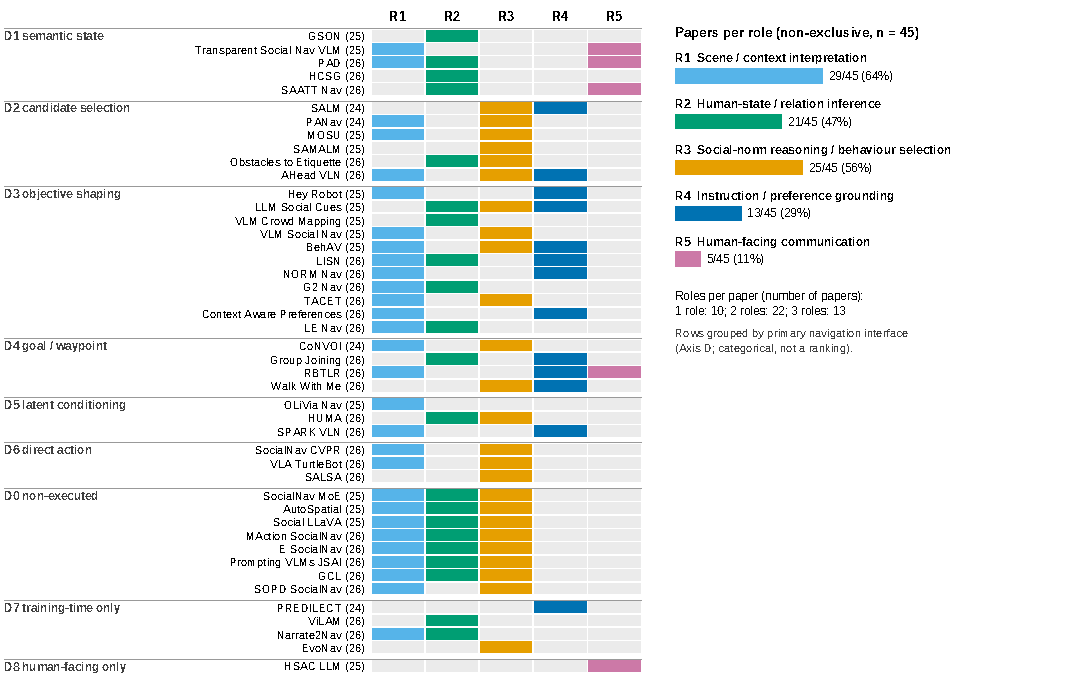
\includegraphics[width=\linewidth,height=0.85\textheight,keepaspectratio]{figures/FigS1_fm_roles}\end{center}
\clearpage
\section*{Fig. S2. Evidence profile per direct paper (Dimension E), grouped by primary navigation interface}
\addcontentsline{toc}{section}{Fig. S2. Evidence profile per direct paper (Dimension E), grouped by primary navigation interface}
\begin{center}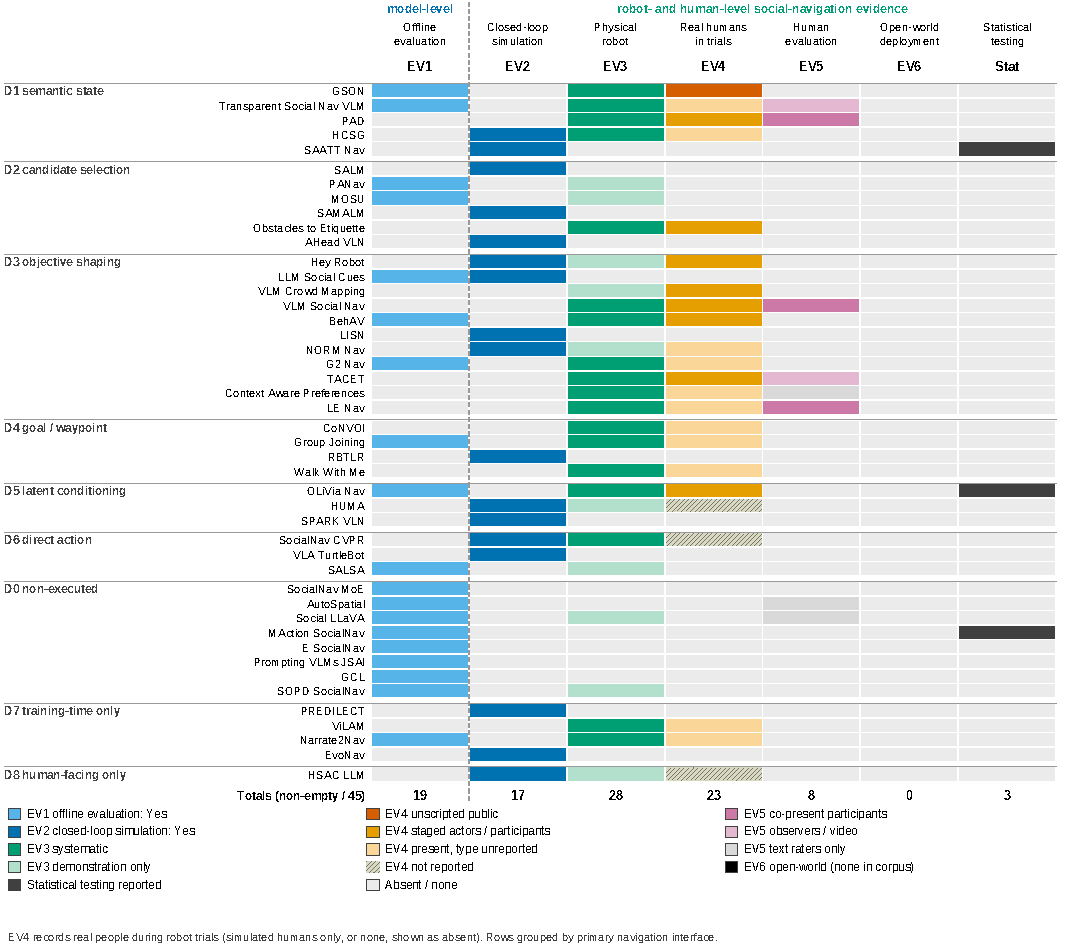
\includegraphics[width=\linewidth,height=0.85\textheight,keepaspectratio]{figures/FigS2_evidence_profile}\end{center}
\clearpage
\section*{Fig. S3. Capability coding per direct paper (Dimension C)}
\addcontentsline{toc}{section}{Fig. S3. Capability coding per direct paper (Dimension C)}
\begin{center}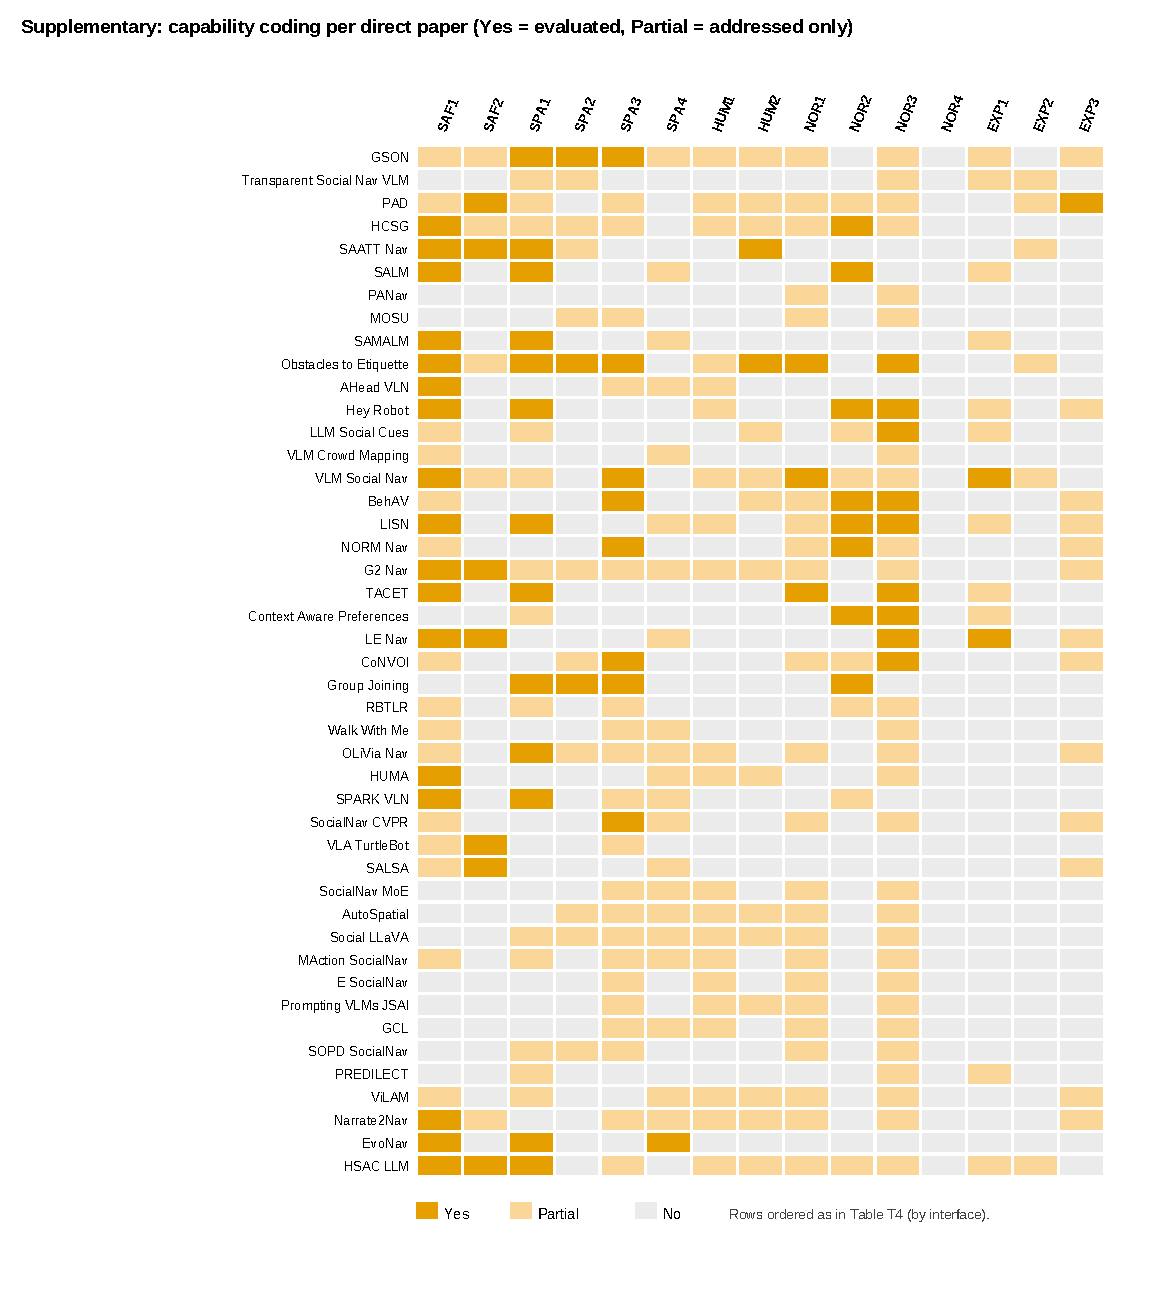
\includegraphics[width=\linewidth,height=0.85\textheight,keepaspectratio]{figures/FigS3_capability_heatmap}\end{center}
\clearpage
\section*{Fig. S4. Dated timeline of the paradigms of social representation. Each band runs from the approximate first appearance of a paradigm to the literature cut-off; markers show representative works at their publication year. Overlapping bands indicate coexistence, not replacement or causal progression}
\addcontentsline{toc}{section}{Fig. S4. Dated timeline of the paradigms of social representation. Each band runs from the approximate first appearance of a paradigm to the literature cut-off; markers show representative works at their publication year. Overlapping bands indicate coexistence, not replacement or causal progression}
\begin{center}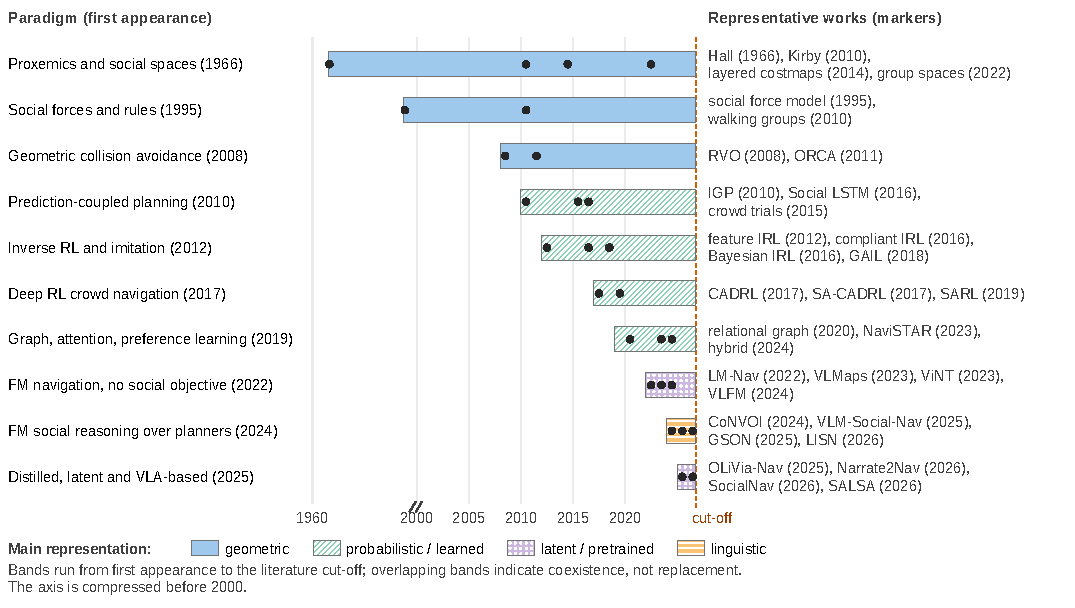
\includegraphics[width=\linewidth,height=0.85\textheight,keepaspectratio]{figures/FigS4_evolution_timeline}\end{center}
\clearpage\renewcommand{\refname}{References cited in Table S5 (pre-FM comparison set)}\addcontentsline{toc}{section}{References cited in Table S5}
\renewcommand{\bibpreamble}{\small Numbering is independent of the main manuscript; every work of the pre-FM comparison set is listed.\par}
\bibliographystyle{elsarticle-num}
\bibliography{references}
\end{document}
